\PassOptionsToPackage{unicode=true}{hyperref} % options for packages loaded elsewhere
\PassOptionsToPackage{hyphens}{url}
%
\documentclass[]{article}
\usepackage{lmodern}
\usepackage{amssymb,amsmath}
\usepackage{ifxetex,ifluatex}
\usepackage{fixltx2e} % provides \textsubscript
\ifnum 0\ifxetex 1\fi\ifluatex 1\fi=0 % if pdftex
  \usepackage[T1]{fontenc}
  \usepackage[utf8]{inputenc}
  \usepackage{textcomp} % provides euro and other symbols
\else % if luatex or xelatex
  \usepackage{unicode-math}
  \defaultfontfeatures{Ligatures=TeX,Scale=MatchLowercase}
\fi
% use upquote if available, for straight quotes in verbatim environments
\IfFileExists{upquote.sty}{\usepackage{upquote}}{}
% use microtype if available
\IfFileExists{microtype.sty}{%
\usepackage[]{microtype}
\UseMicrotypeSet[protrusion]{basicmath} % disable protrusion for tt fonts
}{}
\IfFileExists{parskip.sty}{%
\usepackage{parskip}
}{% else
\setlength{\parindent}{0pt}
\setlength{\parskip}{6pt plus 2pt minus 1pt}
}
\usepackage{hyperref}
\hypersetup{
            pdftitle={Visualiser vos données avec R},
            pdfauthor={Nicolas Casajus, Kevin Cazelles},
            pdfborder={0 0 0},
            breaklinks=true}
\urlstyle{same}  % don't use monospace font for urls
\usepackage[margin=1in]{geometry}
\usepackage{color}
\usepackage{fancyvrb}
\newcommand{\VerbBar}{|}
\newcommand{\VERB}{\Verb[commandchars=\\\{\}]}
\DefineVerbatimEnvironment{Highlighting}{Verbatim}{commandchars=\\\{\}}
% Add ',fontsize=\small' for more characters per line
\usepackage{framed}
\definecolor{shadecolor}{RGB}{248,248,248}
\newenvironment{Shaded}{\begin{snugshade}}{\end{snugshade}}
\newcommand{\AlertTok}[1]{\textcolor[rgb]{0.94,0.16,0.16}{#1}}
\newcommand{\AnnotationTok}[1]{\textcolor[rgb]{0.56,0.35,0.01}{\textbf{\textit{#1}}}}
\newcommand{\AttributeTok}[1]{\textcolor[rgb]{0.77,0.63,0.00}{#1}}
\newcommand{\BaseNTok}[1]{\textcolor[rgb]{0.00,0.00,0.81}{#1}}
\newcommand{\BuiltInTok}[1]{#1}
\newcommand{\CharTok}[1]{\textcolor[rgb]{0.31,0.60,0.02}{#1}}
\newcommand{\CommentTok}[1]{\textcolor[rgb]{0.56,0.35,0.01}{\textit{#1}}}
\newcommand{\CommentVarTok}[1]{\textcolor[rgb]{0.56,0.35,0.01}{\textbf{\textit{#1}}}}
\newcommand{\ConstantTok}[1]{\textcolor[rgb]{0.00,0.00,0.00}{#1}}
\newcommand{\ControlFlowTok}[1]{\textcolor[rgb]{0.13,0.29,0.53}{\textbf{#1}}}
\newcommand{\DataTypeTok}[1]{\textcolor[rgb]{0.13,0.29,0.53}{#1}}
\newcommand{\DecValTok}[1]{\textcolor[rgb]{0.00,0.00,0.81}{#1}}
\newcommand{\DocumentationTok}[1]{\textcolor[rgb]{0.56,0.35,0.01}{\textbf{\textit{#1}}}}
\newcommand{\ErrorTok}[1]{\textcolor[rgb]{0.64,0.00,0.00}{\textbf{#1}}}
\newcommand{\ExtensionTok}[1]{#1}
\newcommand{\FloatTok}[1]{\textcolor[rgb]{0.00,0.00,0.81}{#1}}
\newcommand{\FunctionTok}[1]{\textcolor[rgb]{0.00,0.00,0.00}{#1}}
\newcommand{\ImportTok}[1]{#1}
\newcommand{\InformationTok}[1]{\textcolor[rgb]{0.56,0.35,0.01}{\textbf{\textit{#1}}}}
\newcommand{\KeywordTok}[1]{\textcolor[rgb]{0.13,0.29,0.53}{\textbf{#1}}}
\newcommand{\NormalTok}[1]{#1}
\newcommand{\OperatorTok}[1]{\textcolor[rgb]{0.81,0.36,0.00}{\textbf{#1}}}
\newcommand{\OtherTok}[1]{\textcolor[rgb]{0.56,0.35,0.01}{#1}}
\newcommand{\PreprocessorTok}[1]{\textcolor[rgb]{0.56,0.35,0.01}{\textit{#1}}}
\newcommand{\RegionMarkerTok}[1]{#1}
\newcommand{\SpecialCharTok}[1]{\textcolor[rgb]{0.00,0.00,0.00}{#1}}
\newcommand{\SpecialStringTok}[1]{\textcolor[rgb]{0.31,0.60,0.02}{#1}}
\newcommand{\StringTok}[1]{\textcolor[rgb]{0.31,0.60,0.02}{#1}}
\newcommand{\VariableTok}[1]{\textcolor[rgb]{0.00,0.00,0.00}{#1}}
\newcommand{\VerbatimStringTok}[1]{\textcolor[rgb]{0.31,0.60,0.02}{#1}}
\newcommand{\WarningTok}[1]{\textcolor[rgb]{0.56,0.35,0.01}{\textbf{\textit{#1}}}}
\usepackage{longtable,booktabs}
% Fix footnotes in tables (requires footnote package)
\IfFileExists{footnote.sty}{\usepackage{footnote}\makesavenoteenv{longtable}}{}
\usepackage{graphicx,grffile}
\makeatletter
\def\maxwidth{\ifdim\Gin@nat@width>\linewidth\linewidth\else\Gin@nat@width\fi}
\def\maxheight{\ifdim\Gin@nat@height>\textheight\textheight\else\Gin@nat@height\fi}
\makeatother
% Scale images if necessary, so that they will not overflow the page
% margins by default, and it is still possible to overwrite the defaults
% using explicit options in \includegraphics[width, height, ...]{}
\setkeys{Gin}{width=\maxwidth,height=\maxheight,keepaspectratio}
\setlength{\emergencystretch}{3em}  % prevent overfull lines
\providecommand{\tightlist}{%
  \setlength{\itemsep}{0pt}\setlength{\parskip}{0pt}}
\setcounter{secnumdepth}{5}
% Redefines (sub)paragraphs to behave more like sections
\ifx\paragraph\undefined\else
\let\oldparagraph\paragraph
\renewcommand{\paragraph}[1]{\oldparagraph{#1}\mbox{}}
\fi
\ifx\subparagraph\undefined\else
\let\oldsubparagraph\subparagraph
\renewcommand{\subparagraph}[1]{\oldsubparagraph{#1}\mbox{}}
\fi

% set default figure placement to htbp
\makeatletter
\def\fps@figure{htbp}
\makeatother

\usepackage{booktabs}
\usepackage{amsthm}
\makeatletter
\def\thm@space@setup{%
  \thm@preskip=8pt plus 2pt minus 4pt
  \thm@postskip=\thm@preskip
}
\makeatother
\usepackage[]{natbib}
\bibliographystyle{apalike}

\title{Visualiser vos données avec R}
\author{Nicolas Casajus, Kevin Cazelles}
\date{2020-05-18}

\begin{document}
\maketitle

{
\setcounter{tocdepth}{2}
\tableofcontents
}
\hypertarget{bienvenue}{%
\section*{Bienvenue}\label{bienvenue}}
\addcontentsline{toc}{section}{Bienvenue}

\hypertarget{quest-ce-que-ce-livre}{%
\subsection*{Qu'est-ce que ce livre ?}\label{quest-ce-que-ce-livre}}
\addcontentsline{toc}{subsection}{Qu'est-ce que ce livre ?}

Ce livre est un tour d'horizon des nombreuses possibilités qu'offre le
langage de programmation R pour créer des graphiques. Les sources sont
disponibles à l'adresse suivante: \url{https://github.com/inSileco/VisualiseR}.

Cet ouvrage est sous licence
Creative Commons Attribution-NonCommercial-NoDerivatives 4.0 International License.

Ce site internet est déployé \href{https://github.com/features/actions}{GitHub
Actions}

\hypertarget{future-et-collaboration}{%
\subsection*{Future et Collaboration}\label{future-et-collaboration}}
\addcontentsline{toc}{subsection}{Future et Collaboration}

La première version de ce livre est centré sur faire des graphiques avec les
fonctionnalités de base de R mais le paysage R a bien changé au cours des
dernières années et beaucoup de packages sont devenus très populaires notamment
\texttt{ggplot2}. Nous souhaitons augmenter cette version et introduire ces paquets.

Pour d'autres tours d'horizons des capacités graphiques que R offrent,
le lecteur pourra se reporter à la lecture de différents ouvrages:

\begin{itemize}
\tightlist
\item
  \emph{Data Visualization} par Kieran Healy \url{https://socviz.co/}
\item
  \emph{Fundamentals of Data Visualization} par Claus O. Wilke \url{https://serialmentor.com/dataviz/}
\item
  \emph{R Graphics Cookbook: Practical Recipes for Visualizing Data} par Winston Chang \url{http://shop.oreilly.com/product/0636920023135.do}
\item
  \emph{ggplot2: Elegant Graphics for Data Analysis} par Hadley Wickham
  \url{https://www.springer.com/us/book/9780387981413}
\end{itemize}

Toutes les contributions sont les bienvenues :smile:. Si vous êtes en dehors du
groupe inSileco et que vous avez un compte GitHub, vous pouvez créer une fork ce
répertoire et puis \href{https://help.github.com/articles/creating-a-pull-request-from-a-fork/}{créer un pull request à partir de votre
\emph{fork}}.
Vous pouvez aussi directement \href{https://help.github.com/articles/editing-files-in-another-user-s-repository/}{éditer les fichiers en
ligne}.

Un chapitre est un fichier \texttt{chapitre.Rmd}. Pour en éditer le contenu, l'étendre ou signaler des erreurs, le plus simple est d'ouvrir un \emph{issue} en expliquant ce que vous souhaitez faire ou de détailler l'erreur. Si vous êtes collaborateurs sur le projet, vous pouvez vous assignez la tâche pour signaler au groupe ce sur quoi vous travailler.
Deux \href{https://github.com/inSileco/VisualiseR/projects}{projets} ont été organisés dans le répertoire GitHub (voir \href{https://help.github.com/articles/about-project-boards/}{\emph{About project boards}} pour plus de détails). Pour les utiliser, il suffit de les mentionner au moment de l'ouverture d'un nouvel \emph{issue} est ouvert, on peut en suite les éditer et suivre leur avancement dans l'onglet \emph{project}.

Autres remarques:

\begin{itemize}
\tightlist
\item
  ce livre est édité avec \href{https://github.com/rstudio/bookdownw/}{bookdown}, la documentation est très utile \url{https://bookdown.org/yihui/bookdown/}
\item
  \texttt{code/chapN/} pour les scripts pour le chapitre N;
\item
  \texttt{img/chapN/} pour les figures/images non créés avec R pour le chapitre N;
\item
  \texttt{extdata/} pour les données externes;
\item
  ajouter les references dans \texttt{book.bib};
\item
  suivre les bonnes pratiques pour le code: voir \href{https://github.com/MangoTheCat/goodpractice}{goodpractice}
\item
  donner des noms au \emph{code chunk} afin d'avoir des repères pour faciliter le débogage.
\end{itemize}

\hypertarget{avant-propos}{%
\subsection*{Avant propos}\label{avant-propos}}
\addcontentsline{toc}{subsection}{Avant propos}

Le logiciel R est un environnement de statistiques \emph{open-source} librement distribué sous les termes de la licence publique générale GNU (GPL2). Très puissant pour réaliser n'importe quel type d'analyses statistiques, il s'avère aussi extrêmement performant dans la visualisation des données.
D'ailleurs, dès son apparition au milieu des années quatre-vingt-dix, R était déjà muni d'un module permettant de produire des graphiques.

Utiliser le logiciel R pour produire des graphiques de haute qualité présente un certain nombre d'avantages. Premièrement, chaque composant du graphique peut être modifié, ce qui offre beaucoup de souplesse à l'utilisateur. Deuxièmement, il permet de réaliser l'ensemble du flux de travail (importation de données, manipulation de données, analyses statistiques, représentation graphique et exportation) sur un même support logiciel. Ce qui nous épargne l'apprentissage de différents outils à usage unique. Enfin, son utilisation va trouver toute sa justification lorsqu'une chaîne de traitements devra être répétée un grand nombre de fois (automatisation des tâches).

Au cours des dernières années, de nombreux packages ont été développés pour faciliter la production de graphiques sous R. Parmi eux, citons le package \texttt{lattice} implémenté par Deepayan Sarkar. Ce package s'intéresse spécifiquement à la visualisation de données multivariées. Plus récemment, le package \texttt{ggplot2} développé par Hadley Wickham a énormément gagné en popularité dans les laboratoires de recherches. Il repose sur la grammaire des graphiques (\emph{The Grammar of Graphics}), ouvrage de référence écrit par Leland Wilkinson.

Bien que ces packages soient très intéressants, ils présentent l'inconvénient de dépendre d'un certain nombre de packages additionnels. De plus, leur prise en main peut s'avérer difficile puisqu'ils implémentent souvent des méthodes spécifiques, qui dans le cas de \texttt{ggplot2} peut s'apparenter à un sous-langage R à part entière. L'idée ici n'est pas de dénigrer de tels outils, qui s'avèrent être tout de même puissants et complets. Non, notre objectif est de fournir les clés nécessaires pour produire de graphiques de haute qualité ne nécessitant aucune retouche supplémentaire via des logiciels comme \textit{GNU Image Manipulation Program (GIMP)}, \emph{Adobe Illustrator} ou encore \emph{Adobe Photoshop}. En d'autres termes, vous apprendrez à réaliser des graphiques prêts à être soumis à une revue scientifique.

Cet enseignement est basé sur l'utilisation du système graphique traditionnel de R : le package \texttt{graphics}. Il fait abstraction de tout autre package complémentaire. Le package \texttt{graphics} fait partie des packages de base de R. Sa philosophie est à la fois simple et très puissante : n'importe quel graphique peut être généré sans avoir recours à des packages additionnels. Cela a néanmoins un coût : tout est possible, certes, mais avec un nombre de lignes parfois important, nous le concédons volontiers. Mais, c'est un très bon support pour découvrir l'univers des graphiques et faire connaissance avec leurs éléments constitutifs.

Ce document fait suite à une formation donnée en novembre 2014 à une trentaine d'étudiants gradués de l'Université du Québec à Rimouski. Il est structuré en sept parties. Alors que le premier chapitre illustre les grands types de graphiques réalisables sous R à l'aide des \emph{High-level plotting functions}, le second vous permettra d'éditer un graphe en lui ajoutant des informations avec des \emph{Low-level plotting functions}. Le troisième, probablement le plus long, passe en revue les différents paramètres graphiques. Ainsi, vous apprendrez à jouer avec les couleurs, modifier les marges, les axes, formater une fonte de caractères, etc. Les deux chapitres suivants, un peu plus avancés, vous permettront d'en savoir plus sur les périphériques graphiques et l'exportation de graphes, ainsi que sur la réalisation de graphiques composés (fonction \texttt{layout()}). Le chapitre six est constitué de trois exercices que nous vous invitons à essayer de réaliser avant de consulter le code source présent au chapitre suivant.

Malgré ce programme alléchant, ce document est loin d'être exhaustif, loin s'en faut. Mais, nous voulons croire qu'il répondra à certaines de vos interrogations sur les graphiques sous R. Écrire un document sur les graphiques sous-entend que ce-dit document soit richement illustré. Et c'est le cas. Cependant, les graphiques produits par l'ensemble des lignes de code recensées ici ne sont pas tous présentés. Ceci dans un soucis de clarté de lecture, mais aussi de taille de document. C'est pourquoi nous vous invitons à ouvrir une session R en parallèle de votre lecture, et à recopier les lignes de code. N'hésitez pas à modifier certains paramètres pour voir leurs impacts. La connaissance commence par la curiosité.

Nicolas Casajus, Kevin Cazelles

\hypertarget{remerciements}{%
\subsection*{Remerciements}\label{remerciements}}
\addcontentsline{toc}{subsection}{Remerciements}

A ajouter.

\hypertarget{introduction}{%
\section{Introduction}\label{introduction}}

\begin{itemize}
\item
  Par de nombreux aspects, nous visons dans un âge des données.
\item
  les visualiser est devenu un aspect important que ce soit en science ou dans le traitement de l'actualité.
\item
  Différent langages de programmation offre des libraries de visualisation des données, par example Python et JavaScript. R a ces propres atouts.
\item
  Visualiser les données peut permettre de comprendre mais aussi délivrer un message sur ces dernières. Pour le faire il faut une certaines maîtrise techniques et de la créativité. Sans maîtrise technique, il est difficile de donner corps à sa créativité.
\item
  Ce livre est divisé en quatre parties:

  \begin{enumerate}
  \def\labelenumi{\arabic{enumi}.}
  \tightlist
  \item
    Dans une première partie, nous donnons des éléments de réflexion générale relative à la visualisation des données et R
  \item
    graphics
  \item
    grids
  \item
    web
  \end{enumerate}
\end{itemize}

\hypertarget{part-science-visualisation-et-r}{%
\part{Science visualisation et R}\label{part-science-visualisation-et-r}}

\hypertarget{science-et-graphiques}{%
\section{Science et graphiques}\label{science-et-graphiques}}

Ce chapitre se veut une introduction générale au graphique scientifique. Il s'ouvre sur une brève histoire de la visualisation graphique des données. Le lecteur voyagera des premières cartes rudimentaires du Paléolithique jusqu'à l'époque moderne, marquée par la naissance du \emph{dataviz} et de l'infographie. Il n'existe pas pour l'instant de théorie complètement satisfaisante sur le graphique (même si des efforts ont été entrepris depuis la seconde moitié du XX\textsuperscript{e} siècle), mais nous avons tout de même souhaité fournir au lecteur quelques règles de bon usage dans l'élaboration de graphiques. C'est l'objet de la dernière partie de ce chapitre.

\hypertarget{une-breve-histoire-du-graphique}{%
\subsection{Une brève histoire du graphique}\label{une-breve-histoire-du-graphique}}

Notre époque est marquée par une véritable révolution dans notre manière d'appréhender le monde et les choses qui nous entourent. Ce monde numérique dans lequel nous vivons nous permet de quantifier et d'archiver une quantité phénoménale d'informations. Et les récents développements technologiques fournissent des outils sophistiqués pour analyser et visualiser ces données. C'est dans ce contexte que sont apparues l'infographie et la \emph{data visualisation} (également connue sous le terme de \emph{dataviz}). Longtemps confinés dans des disciplines spécialisées, les graphiques ont envahi notre quotidien (presse écrite et en ligne, journaux télévisés, Internet, etc.) au point que certains abus et erreurs sont régulièrement commis, et les bonnes pratiques dans la conception de graphiques, héritées d'une longue évolution, sont purement écartées au profit de l'esthétisme ou de l'expérience visuelle. Ainsi, il est pertinent de se plonger dans l'histoire du graphique afin d'en dégager les principales innovations et règles de bon usage permettant d'atteindre le but principal de tout graphique : transmettre une information fidèle aux observations, de manière la plus simple sans déformer la réalité.

L'un des plus grands spécialistes de l'histoire du graphique est sans aucun doute Michael Friendly, professeur de psychologie à l'université York au Canada. Il est l'auteur de plusieurs ouvrages dédiés à l'histoire de la visualisation de l'information et des données, mais sa contribution la plus notable est son \emph{Milestones in the History of Thematic Cartography, Statistical Graphics, and Data Visualization}\footnote{\url{http://datavis.ca/milestones/}} (dont l'histoire relatée ici s'est largement inspirée), une chronologie illustrée retraçant la longue histoire de la visualisation des données et des principales innovations. Friendly reconnaît plusieurs époques successives (Friendly 2008), mais dans un soucis de synthèse, nous nous limiterons aux quatre époques suivantes :

\begin{itemize}
\tightlist
\item
  les premiers balbutiements, dont la période précède le XVIII\textsuperscript{e} siècle;
\item
  l'âge d'or, s'étalant du XVIII\textsuperscript{e} siècle à la fin du XIX \textsuperscript{e} siècle;
\item
  l'âge sombre, couvrant la première moitié du XX \textsuperscript{e} siècle;
\item
  la renaissance du graphique, amorcée dès la seconde moitié du XX \textsuperscript{e} siècle.
\end{itemize}

\hypertarget{premiers-balbutiements}{%
\subsubsection{Premiers balbutiements}\label{premiers-balbutiements}}

Il serait tentant de croire que le graphique est un procédé récent, mais les premières tentatives sont très anciennes et trouvent leur origine dans la cartographie et l'astronomie, disciplines indispensables à l'exploration et à la navigation. La plus ancienne carte connue à ce jour date de 13660 calBP\footnote{calBP, pour années \emph{Before Present} calibrées} (période du Paléolithique supérieur) et a été découverte dans la cave d'Abauntz en Navarre espagnole. Il s'agit d'une carte gravée sur une roche et représentant le parcours d'une chasse à venir (ou passée) placé dans le contexte du paysage environ à la cave \citep{Utrilla2009}.

Par la suite, on verra apparaître la première carte du monde connu (Anaximandre de Milet, 550 av. J.-C.), ainsi que la première représentation graphique de la longitude dans une carte figurant une Terre sphérique (Ptolémé, années 150 de notre ère). Au cours des siècles suivants, les découvertes successives dans le domaine de la cartographie conduiront à la réalisation du premier atlas moderne en 1570 par le cartographe néerlandais Abraham Ortelius : le \emph{Teatrum Orbis Terrarum}, composé de 53 cartes (Figure \ref{figortelius}).

\begin{figure}
\centering
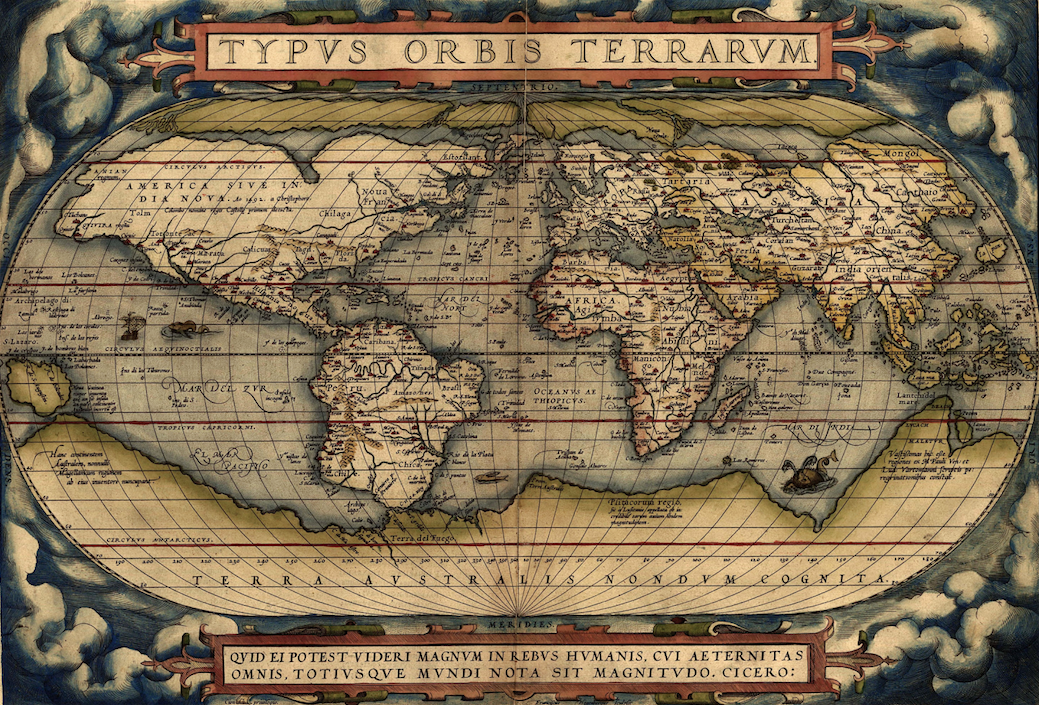
\includegraphics[width=0.95\textwidth,height=\textheight]{img/chap1/ortelius.png}
\caption{Le \emph{Teatrum Orbis Terrarum} d'Abraham Ortelius (1570, domaine publique)}
\end{figure}

C'est donc avec la cartographie que les premières représentations graphiques sont nées et ceci s'explique facilement : une carte ne requière qu'un faible niveau d'abstraction (on représente l'espace dans l'espace). Cependant, des tentatives d'abstraction plus poussées ont été entreprises afin de représenter sous forme de graphiques des informations non spatiales. Ainsi, Nicolas Oresme, évêque de Lisieux aux nombreuses activités (économiste, physicien, mathématicien, astronome, philosophe, etc.) fut le premier à représenter sous forme graphique le rapport entre deux variables (vers 1350). Sans le savoir, il fut le précurseur du système de coordonnées, bien avant René Descartes et son repère cartésien (1637). Un siècle plus tard, Nicolas Krebs (également connu sous le patronyme de Nicolas de Cuse), cardinal et grand penseur allemand à qui l'on doit de nombreux écrits astronomiques, conçoit un graphique théorique dans lequel il représente la vitesse en fonction de la distance.

Par la suite, le XVII\textsuperscript{e} siècle sera marqué par la profusion et l'amélioration des mesures de grandeurs physiques, l'apparition des premiers suivis socio-économiques et le développement de nombreuses théories (géométrie analytique, erreurs et estimations des mesures, statistiques démographiques). La correspondance entre Blaise Pascal et Pierre de Fermat sera à l'origine de la théorie des probabilités, dont le premier ouvrage sur le sujet (\emph{De ratiociniis in ludo aleae}) sera publié par Christian Huygens en 1657.

Fait marquant de ce siècle, la première visualisation graphique de données statistiques en 1644. Celle-ci est l'\oe uvre de Michael Florent van Langren, mathématicien et astronome à la cours du roi Philippe IV d'Espagne ; cette visualisation représente la variation dans la détermination de la longitude entre les villes de Tolède en Espagne et de Rome en Italie.

Ainsi, à la fin du XVII\textsuperscript{e} siècle, les bases seront en place pour développer le début de la pensée graphique et les nouvelles formes graphiques qui conduiront à l'âge d'or du graphique.

\hypertarget{lage-dor}{%
\subsubsection{L'âge d'or}\label{lage-dor}}

Le XVIII\textsuperscript{e} siècle a vu apparaître de nouvelles formes graphiques afin de répondre aux besoins de l'époque. Les cartographes ont commencé à rajouter des informations non géographiques sur leurs cartes, inventant ainsi les isolignes (lignes de même valeur, Edmond Halley, 1701). Ils s'essayent également à la cartographie thématique et les premières cartes géologiques (Johann Friedrich von Charpentier, 1778), topographiques (Marcellin du Carla-Boniface, 1782) et économiques (August Friedrich Wilhelm Crome, 1782) voient le jour.

Le degré d'abstraction est poussé encore plus loin et, avec le développement des statistiques, la visualisation de fonctions théoriques commencent à se répandre (Thomas Bayes, 1763). De nouveaux suivis sont mis en place, et de nouvelles données sont récoltées conduisant à l'invention d'outils (interpolation, ajustement de courbes) et de nouvelles formes visuelles pour les analyser/représenter. C'est en 1765 que Joseph Priestley, théologien, pasteur, pédagogue et enseignant britannique, à qui l'on attribue la découverte de l'oxygène, inventa l'historiographie moderne au moyen de frises chronologiques (Figure \citet{fig:priestley}). Pour la première fois, il représente le temps par l'espace.

\begin{figure}
\hypertarget{fig:priestley}{%
\centering
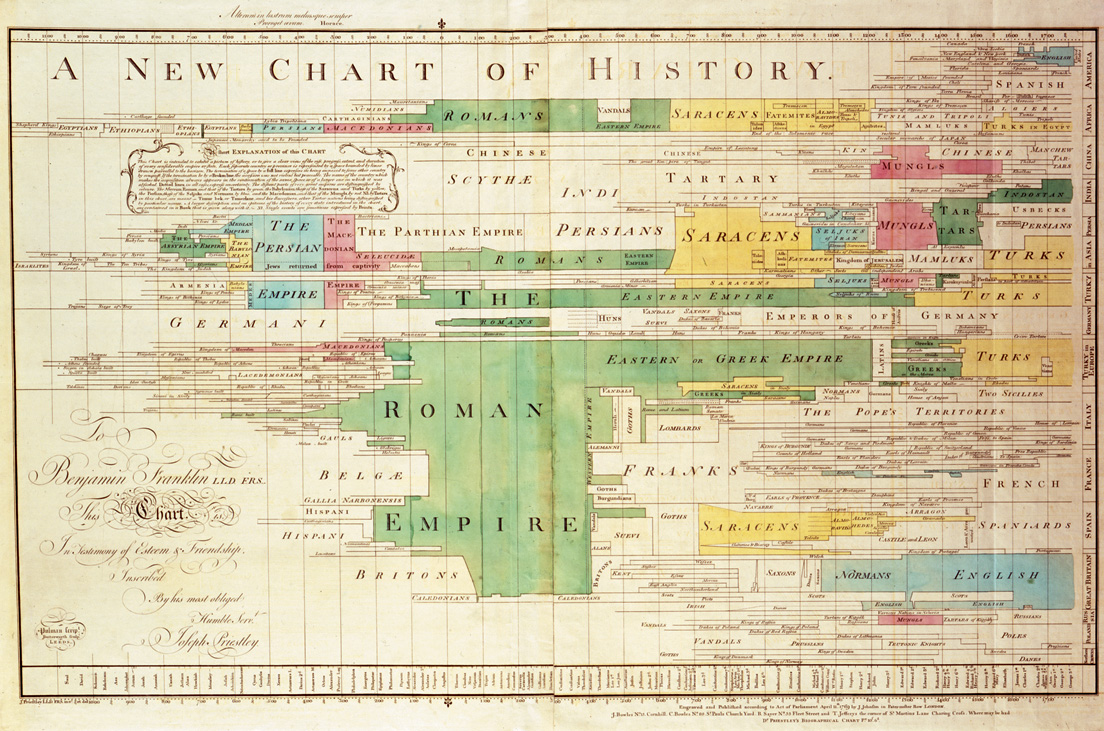
\includegraphics{img/chap1/priestley.jpg}
\caption{\emph{A new chart of History} (Joseph Priestley, 1765, domaine publique)}\label{fig:priestley}
}
\end{figure}

Un autre personnage majeur de ce XVIII\textsuperscript{e} siècle est le mathématicien-philosophe Jean-Henri Lambert. Il est le premier à utiliser les graphiques pour analyser des données empiriques et calculer les pentes de courbes. Il a également développé un système de couleurs pyramidal figurant pour la première fois la notion de saturation. Enfin, il est l'un des premiers à reconnaître l'utilité des graphiques : \emph{a diagram does incomparably better service here than a table}.

Cependant, ces différentes innovations graphiques étaient restreintes à quelques publications éparses, et il faudra attendre la première moitié du XIX\textsuperscript{e} siècle pour que le graphique statistique et la cartographie thématique se démocratisent et connaissent un essor sans précédent. On estime que vers les années 1850, les principales formes graphiques avaient été inventées.

Un des pionniers de cette époque est William Playfair, ingénieur et économiste écossais, à qui l'on doit l'invention de trois graphiques majeurs constituant l'assise de la statistique graphique moderne : le diagramme en barres (1786), probablement inspiré des frises chronologiques de Priestley, le diagramme circulaire, ou camembert (1801), permettant de représenter les proportions relatives des parties au tout, et le graphique linéaire, ou série temporelle (1786), visualisant l'évolution temporelle d'une variable. Ces graphiques sont, encore aujourd'hui, considérés comme des modèles de clarté (Figure \ref{figplayfair}). En 1876, il publie \emph{The Commercial and Political Atlas}, premier ouvrage illustré de graphiques statistiques. Ces graphiques, outre le fait d'introduire de nouvelles formes visuelles, superposent plusieurs informations permettant d'établir le rapport entre plusieurs variables. Vingt ans plus tard, Playfair publiera le \emph{Statistical Breviary} (1801) qui fit découvrir les premiers diagrammes circulaires.

\begin{figure}
\centering
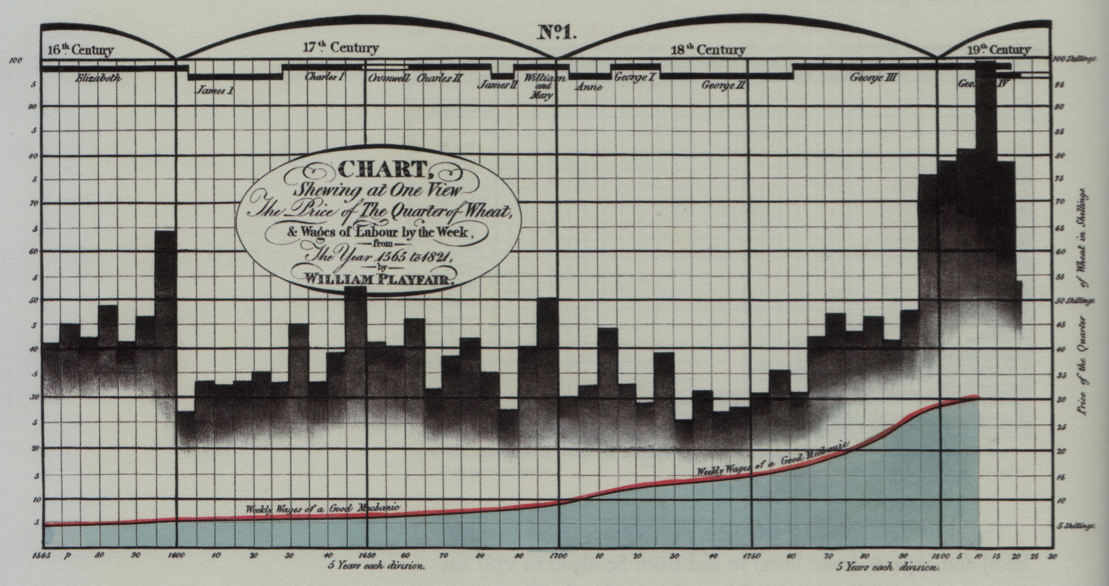
\includegraphics[width=0.95\textwidth,height=\textheight]{img/chap1/playfair.png}
\caption{Graphique représentant le prix du blé et le salaire hebdomadaire de 1565 à 1821 (William Playfair, 1821, domaine publique)}
\end{figure}

Le début de ce XIX\textsuperscript{e} siècle va également être marqué par les travaux du Baron Pierre Charles Dupin, à qui l'on doit la première carte chloroplète (1819) et ceux d'André-Michel Guerry, inventeur du diagramme polaire en 1829, précédant de trente ans les \emph{coxcombs} de Florence Nightingale, souvent reconnue comme étant la première à avoir utiliser cette forme graphique. Guerry, avec Adolphe Quetelet, a énormément contribué à la statistique morale et ses travaux sur la criminologie, largement agrémentés de cartes chloroplètes comparatives, constituent le fondement des sciences sociales modernes.

Dès les années 1820, un nombre croissant de publications scientifiques commence à contenir des graphiques. Cependant, leur usage reste purement descriptif, et il faudra encore attendre plusieurs décennies avant de voir des analyses basées sur les représentations graphiques. Progressivement, la méthode graphique commence à être reconnue dans certains cercles officiels pour ses potentiels dans le domaine de l'économie, du commerce, de l'industrie, de la planification sociale, etc.

Figure de proue de cette seconde moitié du XIX\textsuperscript{e} siècle, l'ingénieur civil français Charles Joseph Minard qui a su faire preuve d'une grande inventivité, notamment dans la synthèse de multiples informations sur un même graphique. Ainsi, il est l'auteur d'une cinquantaine de cartes sur lesquelles sont ajoutés des symboles proportionnels, des diagrammes circulaires, des flux de marchandises, etc. Mais, il est surtout connu pour sa carte figurative des pertes successives en hommes de l'Armée française dans la campagne de Russie en 1812--1813 (Figure \ref{figminard}), dont Edward Tufte n'hésitera pas à dire qu'il consistue le ``meilleur graphique statistique jamais produit''. En effet, ce graphique peut être vu comme un modèle de perfection puisqu'il figure sur un même graphique plusieurs variables : l'emplacement et l'itinéraire de l'armée française indiquant les points de séparation et de ralliement de plusieurs unités, les pertes humaines, la topographie des lieux et la température de l'air.

\begin{figure}
\centering
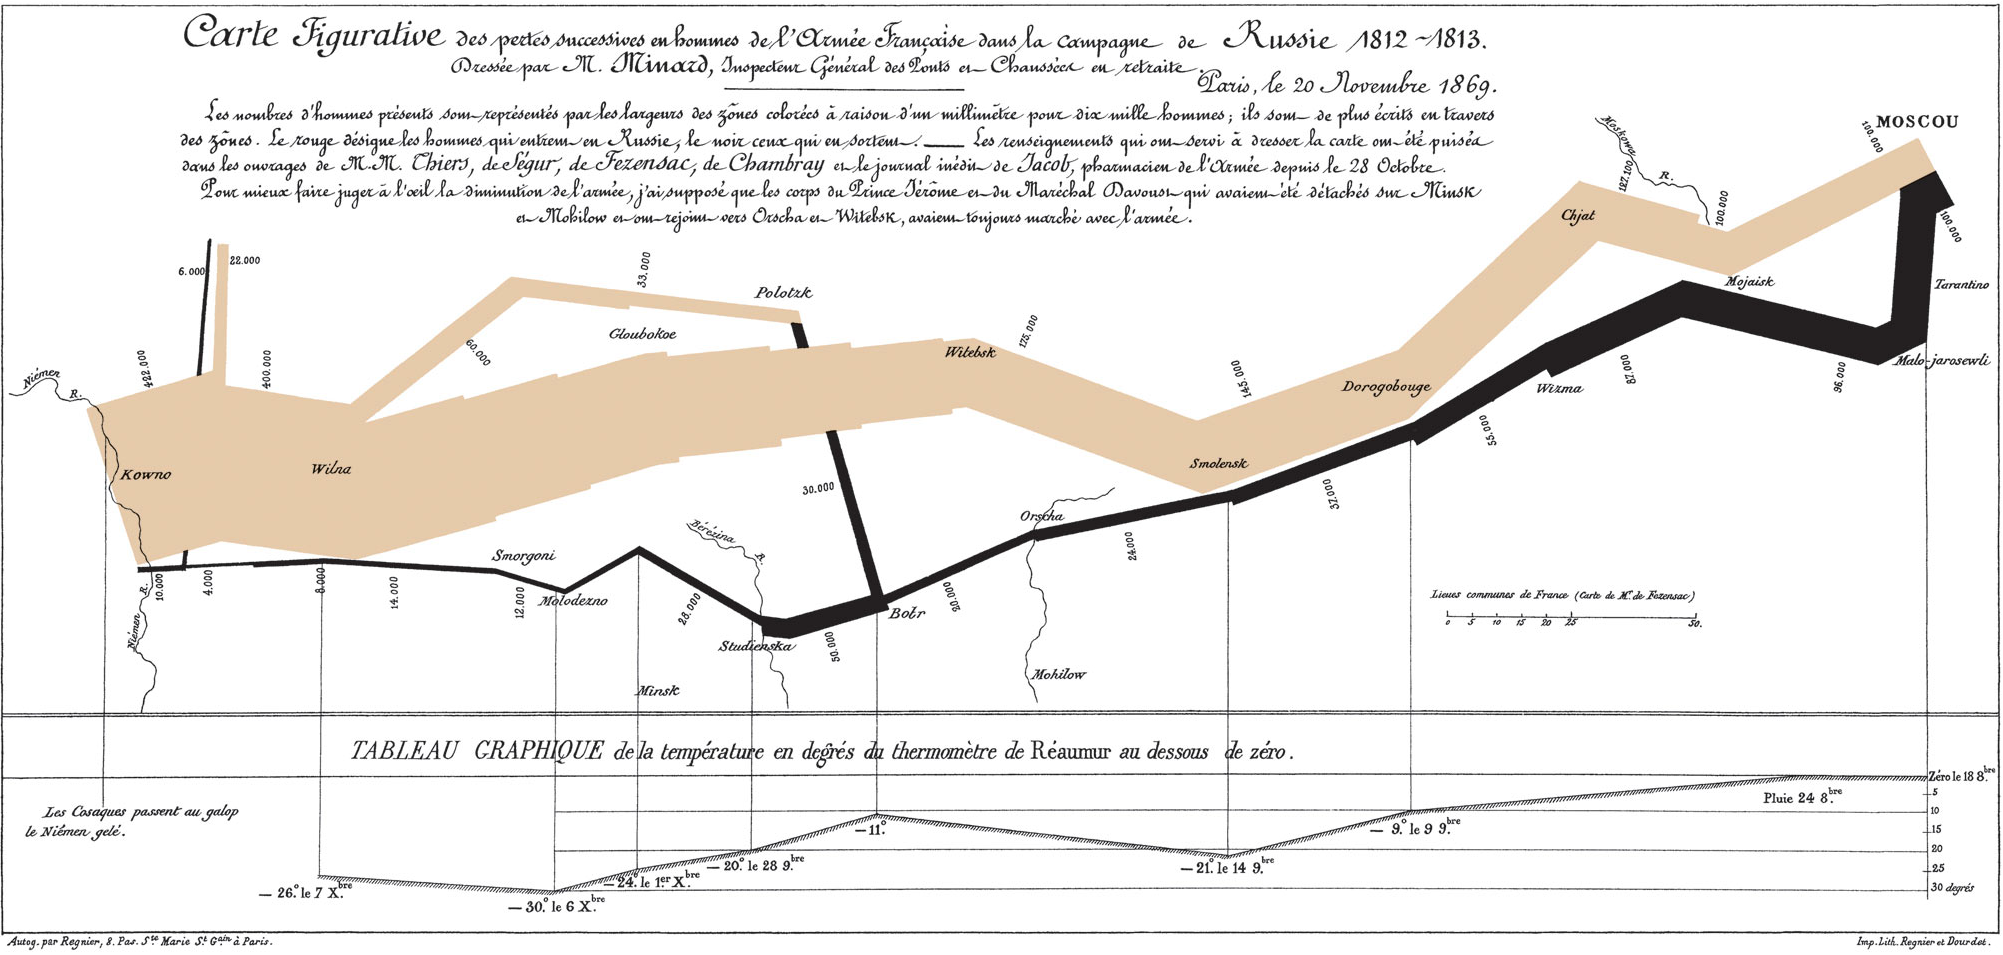
\includegraphics[width=0.95\textwidth,height=\textheight]{img/chap1/minard.png}
\caption{Carte figurative des pertes successives en hommes de l'Armée française dans la campagne de Russie en 1812--1813 (Charles Joseph Minard, 1869, domaine publique)}
\end{figure}

Les innovations vont se poursuivre jusqu'à la fin du XIX\textsuperscript{e} siècle : carte épidémiologique (Snow, 1855), carte météorologique (Galton, 1861), cartogramme (Levasseur, 1868), diagramme illustrant la notion de corrélation (Galton, 1874), graphique en 3D (Perrozzo, 1880), carte anamorphique (Cheysson, 1888), etc. On assiste à la fin de ce siècle aux premiers inventaires des graphiques : écriture de la \emph{Statistique graphique} par Émile Levasseur en 1885, publication annuelle des \emph{Albums de statistiques graphiques} par le Ministère des travaux publics de 1879 à 1897 sous la direction d'Émile Cheysson, synthèse de l'ensemble des graphiques statistiques connus présentée à la \emph{Statistical Society} de Londres, etc. La fin du XIX\textsuperscript{e} siècle sera donc caractérisée par une large diffusion des méthodes graphiques dans différents sphères publiques.

\hypertarget{lage-sombre}{%
\subsubsection{L'âge sombre}\label{lage-sombre}}

\begin{itemize}
\tightlist
\item
  L'entrée dans le XIX\textsuperscript{e} siècle sera\ldots{}
\item
  Malgré cette profusion d'inventions, certains acteurs restent méfiants face à cette nouvelle méthode de travail, notamment les statisticiens britanniques qui continuent à croire que seuls les tableaux de données permettent de décrire correctement la réalité des phénomènes naturels.
\item
  Le XX\textsuperscript{e} siècle : Peu d'innovations, mais des tentatives de normalisation et standardisation\ldots{}
\end{itemize}

\hypertarget{renaissance}{%
\subsubsection{Renaissance}\label{renaissance}}

\begin{itemize}
\tightlist
\item
  Époque moderne : transition avec la section ``Du bon usage des graphiques''
\item
  Ainsi, la visualisation graphique comme procédé de transfert d'informations et de connaissances a longtemps co-évolué avec d'autres disciplines telles les mathématiques, les statistiques, l'astronomie, la médecine, les sciences sociales, les sciences économiques, le commerce, l'industrie, etc. Et, les principales innovations en la matière ont été permises grâce au développement technologique et à des avancées dans la récolte de données.
\end{itemize}

\hypertarget{quest-ce-quun-graphique}{%
\subsection{Qu'est-ce qu'un graphique ?}\label{quest-ce-quun-graphique}}

\begin{itemize}
\tightlist
\item
  Une représentation graphique, en version courte graphique, est un résumé visuel de données mesurées (ou recensées) permettant de dégager des tendances ou toute autre information (cycles, agrégation, connexion, etc.) qu'il serait difficile d'observer dans collection de nombres (stockés le plus souvent dans des tableaux). Il existe de nombreux graphiques différents : c'est la nature des données et le type d'analyses souhaité qui orienteront le choix du graphique à utiliser.
\item
  Simplification de la réalité
\item
  À travers l'histoire du graphique brossée dans la section précédente, différents types de representations graphiques ont été mentionnée (carte, diagramme circulaire, en barres, \ldots\{\}).
\end{itemize}

\hypertarget{un-graphique-pour-quoi-faire}{%
\subsection{Un graphique pour quoi faire ?}\label{un-graphique-pour-quoi-faire}}

\begin{itemize}
\tightlist
\item
  exploration vs.~présentation
\end{itemize}

\hypertarget{du-bon-usage-des-graphiques}{%
\subsection{Du bon usage des graphiques}\label{du-bon-usage-des-graphiques}}

\begin{itemize}
\tightlist
\item
  Dosage design / données
\item
  Choisir le bon type de représentation (adapté aux données et à la question posée)
\item
  Data-ink ratio; 3D; pie chart; line chart pour données continues
\item
  Titre; repère (axe, étiquette); source des données; symbologie;
\item
  Un graphique doit se suffire à lui-même (donc légende et clarté)
\end{itemize}

\hypertarget{uxe0-propos-de-r}{%
\section{À propos de R}\label{uxe0-propos-de-r}}

Étant donné l'engouement autour de R depuis les 10 dernières années, on oublie
que le début de l'histoire remonte au années 70. Dans ce chapitre, nous revenons
sur la naissance et le développement de R: de S depuis les années 70 jusqu'à la
fin des années 90. Nous décrivons ensuite l'émergence de R et la relation qu'il
existe entre S et R. Dans la deuxième partie de ce chapitre, nous dressons un
portait de R en 2019.

\hypertarget{de-s-uxe0-r---50-ans-dhistoire}{%
\subsection{De S à R - 50 ans d'histoire}\label{de-s-uxe0-r---50-ans-dhistoire}}

La description qui suit est une synthèse des trois documents suivants:

\begin{itemize}
\tightlist
\item
  Un article d'un des principaux contributeurs de Richard A. Becker \citep{becker_brief_1994}
\item
  Le chapitre 2 du dernier livre de John M. Chambers, l'un des
  principaux contributeurs de S et maintenant contributeur de R \citep{chambers_extending_2016}
\item
  Le document \emph{R genesis} par Ross Ihaka, l'un des auteurs de R disponible en ligne \url{https://cran.r-project.org/doc/html/interface98-paper/paper_1.html} consulté le 7 février 2019.
\end{itemize}

\hypertarget{le-langage-s}{%
\subsubsection{Le langage S}\label{le-langage-s}}

Pour bien comprendre l'émergence de R, nous revenons sur le contexte dans lequel le langage S a vu le jour et comprendre ce que R lui doit. S est le produit du travail de chercheurs qui
en quête d'un outil performant pour la recherche en statistique dans un monde où l'informatique était en pleine effervescence.

Le résumé que nous faisons de cette émergence débute en 1976, à Murray Hill dans
le New-Jersey (États-Unis), au département de recherche en statistique
informatique des laboratoires Bell\footnote{La lecture de la page Wikipédia dédiée au Laboratoires Bell permet de
  se faire une idée de l'importance des Laboratoires Bell en terme d'innovation,
  les laboratoires Google de l'époque (\url{https://fr.wikipedia.org/wiki/Laboratoires_Bell}, consulté le 31 janvier 2019).}, les calculs sont alors réalisés à
l'aide d'une bibliothèque FORTRAN\footnote{FORmula TRANslator est un langage apparu en 1954 développé par
  John Backus chez IBM (\url{https://fr.wikipedia.org/wiki/Fortran}, consulté le 31 janvier 2019).} SCS (\emph{Statistical Computing
Subroutines}). Un des problèmes posés par cet outil était le temps passé à gérer
les entrées et les sortis au programme qui était long même pour des calculs
simples (une régression linéaire par exemple). Suite à ce constat, les
chercheurs John Chambers, Richard Becker, Doug Dunn et Paul Tukey, décidèrent de
construire un environnement interactif et un nouveau langage afin de faciliter
leur recherche\footnote{\emph{It was the realization that routine data analysis should not require writing Fortran programs that really got S going.} \citep[ p.~2]{becker_s_1984} ``Our primary goal was to bring interactive computing to bear on statistics and data analysis problems.''}. Ce nouveau programme informatique faciliterait
l'utilisation des la bibliothèque SCS grâce à un ensemble d'objets et de
fonctions manipulés à l'aide d'une syntaxe intuitive et permettrait une
exploration visuelle des données à l'aide d'un outil graphique performant.

Suite aux efforts de ces chercheurs, la première version de S (version 1.0) vu le jour en janvier 1977 et fut diffusée au sein des laboratoires Bell. Ainsi, se
constitua la toute première communauté d'utilisateurs de S, celles des chercheurs des laboratoires Bell, communauté restreinte mais très active. La première version de S reflète les avancements en statistique informatique fait depuis les années 50 et met en application les principes que John Chambers développe en 1977 \citep{chambers_computational_1977} :

\begin{enumerate}
\def\labelenumi{\arabic{enumi}.}
\tightlist
\item
  stockage, manipulation des données avant traitement (les trier par exemple);
\item
  utiliser des algorithms efficaces pour traiter les données;
\item
  visualiser les données avec des bibliothèques adéquates.
\end{enumerate}

L'objet de base de S était alors le vecteur (de nombres, de caractères ou bien de variables booléennes), ce qui reste valable avec R aujourd'hui. Une matrice
était aussi un vecteur mais avec un vecteur auxiliaire \texttt{Dim} (ces vecteurs
auxiliaires deviendront plus tard les attributs accessible avec la fonction
\texttt{attributes} dans R). Cette version offrait également la possibilité de créer
des structures dont les différentes composantes étaient appelées grâce à
l'opérateur \texttt{\$} (abondamment utilisé par tous les utilisateurs de R
aujourd'hui, /de même que la fonction \texttt{str} pour avoir un aperçu de l'organisation d'un objet dans R). Ces données étant facilement manipulable via un opérateur d'accès aux différents éléments \texttt{{[}{]}} (subscripting operator) et permet, entre autre, de sous-échantillonner les éléments à partir d'une variable booléenne (ce que les utilisateurs de R font très souvent). Enfin, les graphiques, sujet de ce livre, étaient réalisés grâce à un ensemble de fonctions implémentées dans une bibliothèque distincte appelée GR-Z dont les fonctionnalités sont encore aujourd'hui présentes dans le package R \texttt{graphics}.

L'année suivante, la version 2.0 introduisit notamment les objets de type \texttt{list} pour inclure une collection d'autre objets, amenant ainsi un nouveau type de relation entre les objets. En 1978, les progrès du langage de programmation C, développé dans le même bâtiment aux laboratoires Bell, donnèrent un nouvel élan au langage S. Ce langage développé par Dennis Ritchie et Ken Thompson à la fin des années 60 a été conçu pour être puissant, flexible et
portable, c'est notamment le langage dans lequel est écrit le kernel Linux qui
est un peu partout aujourd'hui\footnote{L'article de Wikipedia est un bon point de départ pour s'informer sur l'histoire de C: \url{https://fr.wikipedia.org/wiki/C_(langage)}, consulté le 21 Décembre 2018.}. La portabilité de C, c'est-à-dire le fait qu'il soit utilisable sur un très grand nombre d'ordinateurs d'architectures différentes, décida les créateurs du langage S (dont les bureaux étaient voisins de celui de Ritchie) d'opter pour une utilisation du langage C et du système UNIX. C'est ainsi qu'en octobre 1979, une version UNIX fut implémentée et devint la version de développement du langage S. R est lui
même écrit en C.

La suite du développement du langage est liée aux retours des premiers utilisateurs de S.
Ces derniers étaient assez limités dans les tâches qu'ils pouvaient accomplir avec S.
Afin d'augmenter les possibilités offertes à l'utilisateur, une boucle \texttt{for} très flexible fut introduite, dont la syntaxe a été conservé par R : \texttt{for\ (i\ in\ index)\ expression}.
De même, une fonction \texttt{apply()} fut ajoutée pour répéter une opération donnée sur chaque colonne ou chaque ligne d'une matrice. Il apparut également une interface de langage pour créer des macros\footnote{Une macro est formée d'un identificateur et d'un morceau de code. Avant l'exécution du programme, toutes les occurrences de l'identificateur dans le code source seront remplacées par le morceau de code auquel elles sont associées.}. Toutes ces innovations sont contenues dans la version de 1984 décrite dans un livre surnommé le \emph{Brown Book}\footnote{Les livres décrivant le langage S sont nommés par des noms de couleurs, en rapport avec la couleur de leur couverture voir \url{http://www.sumsar.net/blog/2014/11/tidbits-from-books-that-defined-s-and-r/}
  consulté le 31janvier 2018.}: \emph{S: An Interactive Environment for Data Analysis and Graphics} \citep{becker_s_1984}. L'année suivante, le livre \emph{Extending the S system} \citep{becker_extending_1985} décrit comment ajouter de nouvelles fonctions au langage S. C'est au même moment que le code source du langage S fut largement distribué sous licence commerciale et éducationnelle.

\hypertarget{le-new-s}{%
\subsubsection{Le « new S »}\label{le-new-s}}

Durant la période 1984--1988, S fut profondément transformé. Alors qu'il était à l'origine dédié à la recherche en statistique, S avait, de fait, de grandes capacités pour manipuler des données, les analyser et les visualiser. Un projet mené par John Chambers fut dédié à l'exploitation de ces atouts pour produire un langage de programmation générale dédié au traitement des données (le \emph{Quantitative Programming Environment}, QPE). En 1986, suite aux avancés du projet, il se posa la question de savoir comment articuler S et QPE. De cette interrogation naquit une troisième version du langage S décrite dans le \emph{Blue Book}: \emph{The New S Language: A Programming Environment for Data Analysis and Graphics} \citep{becker_new_1988}. Les changements apportés étaient d'une telle ampleur qu'il fallut changé le nom : S devint le new S. Beaucoup de fonctions furent réécrites en C. Ainsi, la part de FORTRAN diminua au profit de C pour améliorer la portabilité du new S. A cela s'ajouta la fin de l'interface de langage au profit d'un ensemble très cohérent pour les fonctions. Toutes les fonctions devinrent des objets et les utilisateurs purent alors créer leurs propres fonctions avec la syntaxe que nous connaissons aujourd'hui dans R. Ces fonctions pouvaient avoir un nombre non prédéfini d'arguments et certains de ces arguments pouvaient être passés à d'autres fonctions grâce à l'argument \texttt{...}. Les fonctions écrites en C ou FORTRAN pouvaient être incorporées au new S grâce à des fonctions particulières qui existent toujours dans R: \texttt{.C()}, \texttt{.Fortran()}, etc. Les fonctions graphiques furent également retravaillées et le new S apporta de nouvelles fonctionnalités pour profiter des environnements graphiques, notamment le \emph{X Window System} (X11), apparu en 1984.

En 1992, un nouveau livre, le \emph{White Book}: \emph{Statistical Models in S} \citep{chambers_statistical_1993}, développa les nouvelles fonctionnalités du new S pour travailler sur les modèles statistiques. Les objets de classe \texttt{data.frame} furent introduit : des matrices dont les colonnes peuvent contenir des objets de différentes natures (p.~ex. numérique, texte, booléen, etc.). C'est un objet qui, à notre sense, est vraiment pertinent pour les statistics et sont utilisation est une des forces de R. Avec les \texttt{data.frames} sont introduits les objets de classe \texttt{formula} (caractérisés par l'opérateur \texttt{\textasciitilde{}}) qui permettent de décrire des modèles complexes en très peu de lignes de code. Enfin, la programmation orientée objet\footnote{La programmation orientée objet définit des objets et des méthodes tout en permettant de faire un lien entre les deux. Par exemple, si des objets de classe \emph{point} et d'autres de classe \emph{ligne} sont définis, une méthode, c.-à-d. une fonction, \emph{plot()} peut ensuite être définie pour afficher ces deux objets dans un environnement graphique. La force de la programmation orientée objet sera de permettre un affichage adéquat : des points séparés à l'appel de la méthode \emph{plot} sur l'objet de classe \emph{point} (\emph{plot(point)}) et des points reliés entre eux à l'appel de la méthode \emph{plot} sur l'objet de classe \emph{ligne} (\emph{plot(ligne)}).} prend une place plus importante (il y en avait des prémices en 1988 avec la notamment la fonction \texttt{print()}). Cette approche donne une cohérence et une certaine facilité d'utilisation au langage S et encore aujourd'hui au langage R : on peut ainsi afficher tous nos objets avec la fonction \texttt{print()} dont l'affichage dépendra du type de l'objet (leur classe) sans se poser de question. Le développement d'une approche orientée objet plus formelle est aussi le point central du dernier livre sur S, le \emph{Green Book}: \emph{Programming with Data: A guide to the S Language} qui formalise les objets dit S4 \citep{chambers_programming_1998}.

La création du langage S a soulevé des enjeux techniques majeurs que les développeurs ont surmontés en piochant des idées tantôt dans d'autres langages (p.~ex. l'opérateur assignment \texttt{\textless{}-} provient du langage Algol), tantôt en trouvant des solutions spécifiques à S (p.~ex. l'argument \texttt{...} de certaines fonctions). Le résultat de la vingtaine d'années de développement de S a produit un langage puissant pour la recherche en statistique mais plus généralement pour l'ensemble des opérations du traitement de données. C'est pour ces travaux que John Chambers fut récompensé en 1998 par le prix ACM (\emph{Association for Computing Machinery}). Au début des années 1990, l'histoire de S se prolongea de deux manières: d'un coté la naissance du logiciel libre R et de l'autre, la création d'une version commercial baptisée S-PLUS proposée par l'entreprise américaine TIBCO, qui prit fin en 2009 quand l'entreprise, au vu de la popularité de R, opta pour le développement d'un outil basé sur R : TERR (\emph{TIBCO Enterprise Runtime for R})\footnote{Voir \url{https://en.wikipedia.org/wiki/S-PLUS}, consulté le 7 février 2019.}.

\hypertarget{de-s-uxe0-r}{%
\subsubsection{De S à R}\label{de-s-uxe0-r}}

Au milieu des années 1990, au département de statistiques de l'université d'Auckland, Ross Ihaka et Robert Gentleman font à un constat similaire à celui des chercheurs des Bell Labs firent des années plus tôt : le besoin d'un outil logiciel performant pour le domaine. Bien que les premières versions du langage S étaient facilement accessible aux milieux universitaires, l'outil n'était pas libre et difficile à mettre en place sur les machines Macintosh avec lesquelles ces chercheurs travaillaient. Les deux chercheurs se lancèrent alors dans le développement d'un nouvel outil inspirés par le new S mais aussi le Scheme\footnote{Scheme est apparu dans les années 1970 au Massachusetts Institute of Technology (MIT) grâce au travail de Guy Lewis Steel et Geral Jay Sussman.} comme ils expliquent dans leur article de 1996 \citep{ihaka_r_1996}. Ainsi naquit le langage R, fortement influencé par le new S mais avec un soupçonné de quelque principe de Scheme, notamment pour la gestion de la mémoire et de la portée des variables. Il faut ajouter à ces changements, des travaux sur l'interface graphique avec l'implémentation des couleurs, la texture des lignes, la possibilité d'introduire des formules mathématiques sur un graphique et la mise en page des graphiques. Ces deux derniers éléments sont le fait des travaux de thèse de Paul Murrel qui a travaillé sur la gestion des graphiques sous R\footnote{Il est notamment l'auteur de l'ouvrage \emph{R graphics}{[}ref{]}.}.

En août 1993, les auteurs annoncent la mise à disposition de leur travail R sur la liste de diffusion S-news. Comme il a été fait pour S, R a mis en place le moyen de s'enrichir des retours des utilisateurs. L'un des utilisateurs particulièrement actif, Martin Mächler de l'Eidgenössische Technische Hochschule Zürich (ETH Zürich)\footnote{Avec Friedrich Leisch, de la même institution, ils s'étaient rapprochés du projet en apportant des corrections à des bugs.}, devint un acteur important du projet et incita les chercheurs de Nouvelle-Zélande à rendre leur logiciel libre. C'est ainsi que R fut mis à disposition de tous sous la licence publique générale GNU-GPL dès 1995, d'où son surnom de \emph{GNU S}. L'article de 1996 \emph{R: A Language for Data Analysis and Graphics} qui met au grand jour l'existence de R \citep{ihaka_r_1996}. Ces deux événements combinés donnent une impulsion forte au langage R. De fait, ces dispositions allaient accroître le nombre d'utilisateur, et la distribution et la communication allaient en être profondément changées. En mars 1996, Mächler créa la première liste de diffusion spécifique à R : R-tester, qui fut divisée en trois l'année suivante : R-announcement, R-help et R-devel. Pour organiser le développement de R, il devint pressant d'avoir un système d'archivage dédié à R. Ce fut Kurt Hornik de l'université Technique de Vienne\footnote{\url{https://stat.ethz.ch/mailman/listinfo}} qui s'en chargea et mis au point un système qui évoluera pour donner le CRAN actuel. Le nombre de retours sur R devint tel que Ihaka, Gentleman et Mächler ne suffisaient plus pour assurer convenablement le développement du langage. Ils décidèrent alors de partager cette tâche avec Doug Bates, Peter Dalgaard, Kurt Hornik, Friedrich Leisch, Thomas Lumley, Paul Murrell, Heiner Schwarte et Luke Tierney : l'équipe de développement \emph{R-Core}\footnote{Ils étaient 11 initialement, 16 en 2002 et 21 en août 2015.} se formait.

Une manière simple et efficace pour prendre conscience de l'évolution de R de 1997 à nos jours est de fouiller dans les archives du site internet du CRAN. Par exemple, dans le fichier \emph{README} de la version R.0.49, on peut lire qu'en avril 1997, une bonne partie des fonctions du \emph{Blue book} \citep{becker_new_1988} et du \emph{White Book} \citep{chambers_statistical_1993} étaient déjà implémentées. La reconnaissance formelle du groupe R-Core est présente dans la version R.0.60 de décembre 1997. L'implémentation d'une grande partie des fonctionnalités de S conduisit à la version 1.0.0 de R, le 29 février 2000. Pour l'anecdote, le premier CD-ROM fut donné à John Chambers qui avait rejoint l'équipe du R-Core en 1998. En janvier 2001, c'est la première version d'un journal dédié à R (alors appelé R news) qui fut publiée (voir \url{https://www.r-project.org/doc/Rnews/Rnews_2001-1.pdf}, consulté le 12 décembre 2018). En décembre 2001, avec la version 1.4, ce sont les objets S4 qui sont implémentés. Ces derniers étaient décrits dans le \emph{Green Book} \citep{chambers_programming_1998} et procurèrent à R un cadre beaucoup plus formel pour faire de la programmation orientée objet. En octobre 2004, la version 2.0 était distribuée, et introduit pour la première fois le \emph{lazy loading} (chargement paresseux) permettant d'améliorer les performances de R: lorsqu'un package (extension) est chargé, il est rare que toutes ses fonctionnalités soient exploitées en même temps, R crée des bases de données pour stocker et répertorier le code qui ne sera alors chargé qu'au premier appel de l'utilisateur. En avril 2013, la gestion des valeurs d'indexation des vecteurs supérieurs à 2\textsuperscript{31} pour les systèmes exploitant des processeurs à 64 bits augmenta les performances de R en termes de mémoire et nous amena aux versions 3.x.x. Pour les lecteurs qui cherchent à obtenir des détails techniques relatifs aux fonctionnements internes de R, il est à noter qu'une documentation couvrant ces aspects est disponible en ligne \url{https://cran.r-project.org/doc/manuals/r-release/R-ints.html} (consulté le 21 décembre 2018). De plus, l'ensemble des changements associés aux différentes versions de R depuis Juin 2009 sont rapportés dans les différent numéros du \emph{R Journal} dont les numéros sont visibles en ligne à l'adresse suivante \url{https://journal.r-project.org/} (consulté le 21 décembre 2018) et il est possible de remonté jusqu'en 2001 en consultant les différents numéros de \emph{R News} disponible à \url{https://journal.r-project.org/archive/r-news.html}
(consulté le 21 décembre 2018).

\begin{longtable}[]{@{}lll@{}}
\caption{Date de sortie des différentes version sur le CRAN (voir \url{https://cran.r-project.org/} pour une list complète).}\tabularnewline
\toprule
Version & Date de publication & Notes\tabularnewline
\midrule
\endfirsthead
\toprule
Version & Date de publication & Notes\tabularnewline
\midrule
\endhead
R-0.49 & 23 avril 1997 & première version accessible sur le CRAN\tabularnewline
R-1.0.0 & 29 février 2000 & pour l'année millénaire et donc bissextile\tabularnewline
R-1.2.1 & 22 juin 2001 & premier volume de R news\tabularnewline
R-2.0.0 & 4 octobre 2004 & introduit le \emph{lazy loading}\tabularnewline
R-3.0.0 & 3 avril 2013 & optimization pour les processeurs à 64 bits\tabularnewline
R-3.5.0 & 23 avril 2018 & tous les packages sont\tabularnewline
R-4.0.0 & 24 avril 2020 & pour les 20 ans de R\tabularnewline
R-4.0.0 & 24 avril 2020 & version utilisée pour ce livre\tabularnewline
\bottomrule
\end{longtable}

\hypertarget{r-aujourdhui}{%
\subsection{R aujourd'hui}\label{r-aujourdhui}}

\hypertarget{mais-r-cest-quoi-au-juste}{%
\subsubsection{Mais R c'est quoi au juste?}\label{mais-r-cest-quoi-au-juste}}

Les premières phrases de l'article en français consacré à R sur Wikipedia définissent R ainsi:

\begin{quote}
R est un langage de programmation et un logiciel libre destiné aux statistiques et à la science des données soutenu par la R Foundation for Statistical Computing. R fait partie de la liste des paquets GNU3 et est écrit en C (langage), Fortran et R.\footnote{\url{https://fr.wikipedia.org/wiki/R_(langage)} consulté le 22 décembre 2018.}
\end{quote}

De même sur la page du projet R, on peut lire:

\begin{quote}
R is a free software environment for statistical computing and graphics. It compiles and runs on a wide variety of UNIX platforms, Windows and MacOS.\footnote{\url{https://fr.wikipedia.org/wiki/R_(langage)} consulté le 22 décembre 2018.}
\end{quote}

\begin{quote}
{[}Traduction{]} R est un environment logiciel pour la statistique computationnelle et les graphiques. Il peut être compilé et exécuté sur un grand nombre de plateforme UNIX, Windows et MacOS.
\end{quote}

R est donc un langage: permet d'écrire du code (\emph{en} R) mais aussi en logiciel qui permet d'exécuter du code R (\emph{dans} R) pour faire des statistiques et des graphiques.
R est un langage dit interprété.

\begin{figure}
\centering
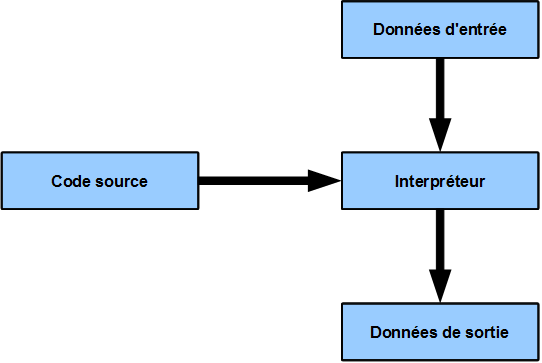
\includegraphics{img/chap2/schema_interpreted_FR.png}
\caption{Langage interprété (voir \url{http://www.france-ioi.org/algo/course.php?idChapter=561\&idCourse=2368})}
\end{figure}

Par opposition à un langage compilé comme C (le langage dans lequel R est écrit).

\begin{figure}
\centering
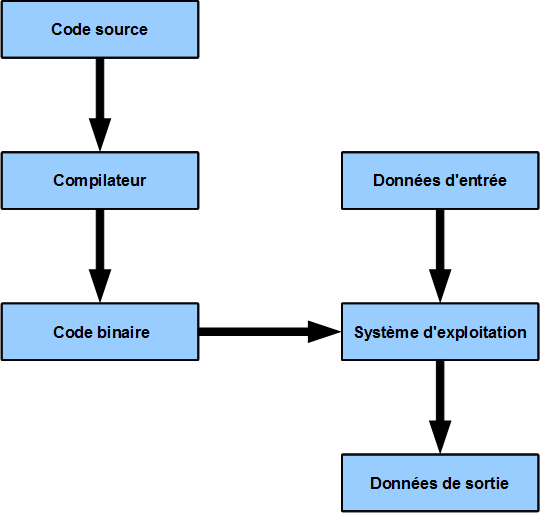
\includegraphics{img/chap2/schema_compiled_FR.png}
\caption{Langage compilé (voir \url{http://www.france-ioi.org/algo/course.php?idChapter=561\&idCourse=2368})}
\end{figure}

Concrètement R est un ensemble de fichiers. Dans la version 3.5.2, il y, entre autre, 559 fichiers \texttt{.c}, 289 fichiers \texttt{.po} (pour la traduction en différente langues), 196 fichiers \texttt{.h} (headers utilisé avec C), 86 fichiers \texttt{.f} (FORTRAN) et 2346 fichiers \texttt{.R}. À l'installation de R, tous ces fichiers sont compilés de sorte que vous pouvez utiliser R dans un terminal.

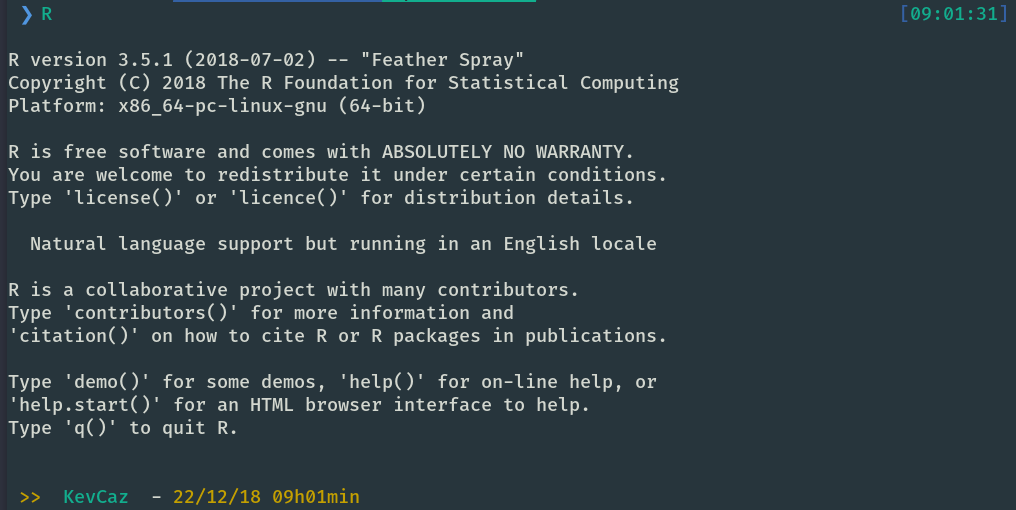
\includegraphics{img/chap2/screenshotR.png}

Un terminal avec R permet d'utiliser toutes les fonctionnalités de R mais n'est suffisant pour programmer de manière efficace. C'est pourquoi on utilise une interface de développement, R propose une telle interface mais la plus populaire de nos jours est RStudio\footnote{\url{https://www.rstudio.com/products/rstudio/download/} consulté le 24 décembre 2018.}, nous y reviendrons.

\hypertarget{un-ensemble-dacteurs}{%
\subsubsection{Un ensemble d'acteurs}\label{un-ensemble-dacteurs}}

Il y a aujourd'hui une myriade d'acteurs qui gravitent autour de R de sorte qu'il est difficile de s'y retrouver et de comprendre qui fait quoi. Ce qui suit est une tentative de mettre un peu d'ordre dans toutes ces informations.

\hypertarget{la-r-fondation-et-la-r-development-core-team}{%
\paragraph{\texorpdfstring{La R fondation et la \emph{R Development Core Team}}{La R fondation et la R Development Core Team}}\label{la-r-fondation-et-la-r-development-core-team}}

Le plus simple pour se repérer est de consulter sur la page du projet R: \url{https://www.r-project.org/} (consulté le 23 décembre 2018). Sur cette page, on trouve notamment un lien vers la Fondation R\footnote{\url{https://www.r-project.org/foundation/} consulté le 23 décembre 2018}. Il s'agit d'une organization a but non lucratif qui a été créé par les membres de la \emph{R Development Core Team} pour pérenniser le développement de R et c'est finalement une distinction. Les membres de la fondation sont des personnes reconnus pour les efforts dans le développement de R, c'est une distinction honorifique. Quand aux membres de la \emph{R Development Core Team}, ce sont les développeurs qui ont un accès d'écriture au code source de R. Ce sont les premiers membres listés quand vous tapez \texttt{contributors()} dans une console R. Ils fixent les bogues dans les fonctionnalités de base de R\footnote{Les bogues peuvent être rapportés par les utilisateurs sur bugzilla \url{https://bugs.r-project.org/bugzilla3/}.} et rendent disponibles les nouvelles versions de R sur le CRAN.

\hypertarget{le-cran}{%
\paragraph{Le CRAN}\label{le-cran}}

Toujours sur la page du projet R, il y a un lien vers le CRAN (\emph{Comprehensive R Archive Network}) qui est le site Internet où sont archivées les différentes versions de R ainsi que les packages qui ont été soumis au CRAN et qui ont été acceptés. C'est également une source privilégiée de resources avec de nombreux manuels et ouvrages pour se familiariser avec R (voir les sections \emph{Manuals} et \emph{Contributed} sur \url{https://cran.r-project.org/}). Le CRAN est maintenu par une équipe de volontaires, la ``CRAN team'', qui met à jour le site et s'occupent des soumissions des packages. Pour être plus exact, le CRAN est une collection de sites miroirs dont les contenus sont synchronisés avec le site du CRAN maintenu à la Wirtschaftsuniversität à Vienne. En 2002, il existait 12 sites miroirs, et en
décembre 2018, 164 sites miroirs se répartissent les téléchargements de R et de ses packages, ainsi que l'archivage des différentes versions. Comment avoir accès à ces chiffres? Avec R bien sur:

\begin{Shaded}
\begin{Highlighting}[]
\CommentTok{# lit le code source de la page qui référence les miroirs}
\NormalTok{mir <-}\StringTok{ }\KeywordTok{readLines}\NormalTok{(}\StringTok{"https://cran.r-project.org/mirrors.html"}\NormalTok{)}
\CommentTok{# compte le nombre de ligne qui contiennent des liens internet avec}
\CommentTok{# http dans le lien (il y a d'autres liens sur la page mais sans http)}
\KeywordTok{sum}\NormalTok{(}
  \KeywordTok{unlist}\NormalTok{(}
    \KeywordTok{lapply}\NormalTok{(mir, grepl, }\DataTypeTok{pattern =} \StringTok{"<a href=}\CharTok{\textbackslash{}"}\StringTok{http"}\NormalTok{)}
\NormalTok{  )}
\NormalTok{)}
\end{Highlighting}
\end{Shaded}

\hypertarget{le-consortium-r}{%
\paragraph{Le consortium R}\label{le-consortium-r}}

Une autre entité qui a vu le jour récemment est le consortium R :
\url{https://www.r-consortium.org/} (consulté le 24 décembre 2018). Comme indiqué
par le site Internet dédié

\begin{quote}
The central mission of the R Consortium is to work with and provide support to the R Foundation and to the key organizations developing, maintaining, distributing and using R software through the identification, development and implementation of infrastructure projects.
\end{quote}

\begin{quote}
{[}Traduction{]} La mission centrale du consortium R est de collaborer avec la Fondation R et les organisation majeures qui développent, maintiennent, distribuent et utilisent le logiciel R à travers l'identification,. le development et l'implémentation de projet infrastructure.
\end{quote}

Ce projet est l'un des projets Open Source supporté par la Fondation Linux: \url{https://www.linuxfoundation.org/projects/} (consulté le 22 décembre 2018). Pour
voir les soutiens financiers du consortium R rendez vous sur cette page \url{https://www.r-consortium.org/members}.

\hypertarget{rstudio}{%
\paragraph{RStudio}\label{rstudio}}

Il s'agit d'un acteur tellement connu qu'il y a une parfois une confusion
entre R et RStudio. RStudio, Inc.\footnote{\url{https://www.rstudio.com/} consulté le 24 décembre 2018.} une entreprise fondé par Joseph J. Allaire qui développe un environment de développement\footnote{\url{https://fr.wikipedia.org/wiki/Environnement_de_d\%C3\%A9veloppement} consulté le 24 décembre 2018.} pour R et propose des services aux entreprises basés sur R (voir la section \emph{Products} sur leur site Internet). En décembre 2018, RStudio comptait près d'une centaine de salariés \url{https://www.rstudio.com/about/} dont de nombreux programmeurs parmi les plus actifs au sein de la communauté des utilisateurs de R (Hadley Wickham et Yihui Xie par exemple). RStudio est connu pour son interface de développement du même nom et pour la qualité des packages R que les salariés de RStudio développements. C'est un modèle économique classique dans le monde de l'opensource\footnote{\url{https://medium.com/france/business-model-de-l-open-source-a2d8e53181f7} consulté le 24 décembre 2018}: une entreprise propose des services autour d'un logiciel qu'elle contribue activement à améliorer et dont elle fait une promotion active (étant donné que c'est la qualité du logiciel qui va déterminer son nombre de clients). La contribution de RStudio à R est considérable, les packages qu'elles contribuent à développer son parmi les plus utilisés\footnote{voir le compte GitHub de RStudio \url{https://github.com/rstudio} (consulté le 24 décembre 2018)}.

\hypertarget{ropensci}{%
\paragraph{rOpenSci}\label{ropensci}}

Sur le site Internet de rOpenSci\footnote{\url{https://ropensci.org/about/} consulté le 26 décembre 2018 ou on apprend aussi que que rOpenSci est sponsorisé par NUMFOCUS (\url{https://numfocus.org/}).}, on peut lire:

\begin{quote}
rOpenSci fosters a culture that values open and reproducible research using shared data and reusable software.
\end{quote}

\begin{quote}
{[}Traduction{]} rOpenSci encourage une culture qui promeut la recherche ouverte et reproductible qui utilise des données partagées et des logiciels réutilisables.
\end{quote}

Pour cela l'équipe de rOpenSci crée et révise des packages\footnote{\url{https://ropensci.org/packages/} consulté le 26 décembre 2018.} qui facilitent la recherche ouverte et reproductible. Il peut s'agir de packages qui interrogent des bases de données accessibles en ligne via des interfaces spécifiques, un exemple emblématique de cette catégorie est \texttt{taxize}\footnote{voir \url{https://github.com/ropensci/taxize} et \url{https://ropensci.org/tutorials/taxize_tutorial/} consultés le 26 décembre 2018.}, véritable couteau suisse pour obtenir des informations taxonomiques
ou encore de packages qui améliore le flux de travail comme \texttt{drake}\footnote{\url{https://github.com/ropensci/drake} consulté le 26 décembre 2018.}. rOpenSci anime également un blog\footnote{\url{https://ropensci.org/blog/} consulté le 26 décembre 2018.} sur lequel on trouve des posts présentant les différents packages révisés par cette organisation et des tutoriels pour apprendre à réaliser certaines manipulations de données avec R. Enfin, rOpenSci anime une communauté\footnote{\url{https://ropensci.org/community/} consulté le 26 décembre 2018.} dynamique et propose des \emph{community calls}, c'est-à-dire des présentations sur certains aspects de R que l'on peut joindre en direct ou consulté l'archive associée\footnote{\url{https://ropensci.org/commcalls/} consulté le 4 janvier 2019.}.

\hypertarget{la-communautuxe9-des-utilisateurs-de-r}{%
\paragraph{La communauté des utilisateurs de R}\label{la-communautuxe9-des-utilisateurs-de-r}}

La myriade des utilisateurs de R est sans aucun doute l'acteur le plus important
car cette communauté :

\begin{enumerate}
\def\labelenumi{\arabic{enumi}.}
\tightlist
\item
  augmente les fonctionnalités de R en créant des packages;
\item
  échanges des informations relative à R par la création et l'édition de manuels, de livres, de blogs, etc.;
\item
  s'auto-organize à travers des communautés locales d'utilisateurs;
\item
  s'auto-supporte: les utilisateurs répondent rapidement aux questions d'autres utilisateurs.
\end{enumerate}

Tout le monde peut écrire des packages ou partager son expérience avec R et de fait, beaucoup d'utilisateurs le font. Il existe un grand nombre de bloggers qui produisent une multitude de posts sur différents aspects de R\footnote{Nous avons notre propre blog qui traite souvent de R \url{https://insileco.github.io/}.}. C'est une resource riche et diversifiée et il existe une plateforme très utile qui les rassemble\footnote{\url{https://blog.feedspot.com/r_programming_blogs/} pour une classification subjective.}: R-bloggers\footnote{\url{https://www.r-bloggers.com/} consulté le 26 décembre 2018.}. De nombreux indices attestent que la communauté des utilisateurs de R est en croissance. Par exemple, le nombre de groupes d'utilisateurs de R est en très forte hausse comme le montre la couverture du dernier livre de John Chambers qui compare le nombre de groupe d'utilisateurs de R entre 2010 et 2015.

\begin{figure}
\centering
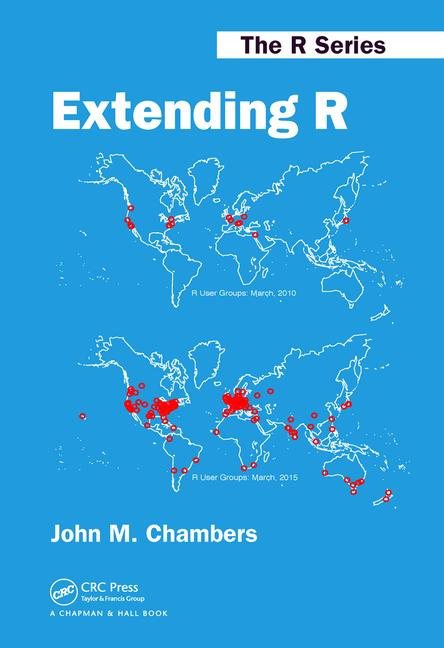
\includegraphics{img/chap2/extendingR.jpg}
\caption{Couverture de \emph{Extending R} \citep{chambers_extending_2016}. Pour une liste qui recense ces communautés, voir \url{https://jumpingrivers.github.io/meetingsR/index.html} (consulté le 26 décembre 2018)}
\end{figure}

On peut aussi regarder la croissance du nombre de packages qui dépassait 10,000 en 2016 (voir \url{https://blog.revolutionanalytics.com/2017/01/cran-10000.html} consulté le 26 décembre 2018). L'explosion du nombre de packages R hébergés sur GitHub\footnote{un site Internet qui peut être décrit comme une forge logiciel basée sur le logiciel \texttt{git} qui rend la programmation collaborative particulièrement efficace.} (près de
45000 à la fin décembre 2018 d'après \url{https://rdrr.io/}). Un autre indice est la popularité du tag ``R'' sur la plateforme d'échange \emph{stack overflow} où les utilisateurs posent des questions auxquelles répondent d'autres utilisateurs. C'est d'ailleurs la popularité sur Github et sur stack overflow que le site internet \href{https://redmonk.com/}{redmonk} évaluent la popularité des langage de programmation et en janvier 2018, R était classé 12\textsuperscript{ème}.

\begin{figure}
\centering
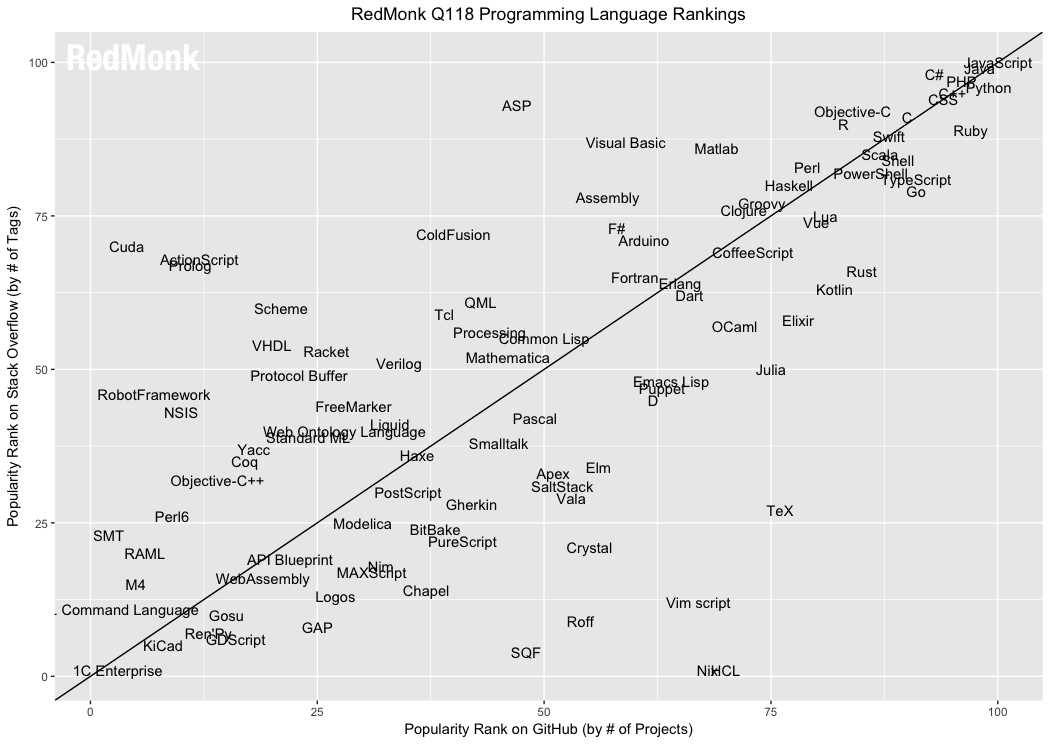
\includegraphics{img/chap2/rank_18.png}
\caption{Le résultat du sondage redmonk en janvier 2018, voir \url{https://redmonk.com/sogrady/2018/03/07/language-rankings-1-18/} consulté le 26 décembre 2018.}
\end{figure}

Un dernier indice de l'accroissement de la popularité de R chez les écologistes que nous sommes est la forte demande en formation de nos collègues. R figure incontestablement parmi les outils computationnels les plus utilisés pour la statistique et la science des données de manière générale. De plus en plus d'écologues apprennent R avec un niveau de formation de de plus en plus avancé.

\hypertarget{une-documentation-abondante-et-facilement-accessible}{%
\subsubsection{Une documentation abondante et facilement accessible}\label{une-documentation-abondante-et-facilement-accessible}}

Les acteurs mentionnés ci-dessus précédemment produisent une documentation
abondante aussi bien pour débuter avec R, réaliser des tâches spécifiques avec R (au moyen de packages dédiés) que pour programmer efficacement avec R et développer ses propres packages\footnote{nous maintenons une liste de resource à l'adresse suivante: \url{https://insileco.github.io/wiki/usefulr/}.}.

Pour les débutants, un moyen rapide de mettre le pied à l'étrier est de consulter les sections \emph{Manuals}, \emph{Books} de la page Internet du projet R (\url{https://www.r-project.org}) et la section \emph{Contributed} qui propose des introductions à R dans différentes langues. Cette page n'est malheureusement plus mise à jour mais on y trouve, par exemple, l'\emph{Introduction à R} de Julien Barnier (voir \url{http://alea.fr.eu.org/pages/intro-R}). On peut aussi citer des des acteurs de formation très populaires qui offrent des formations dédiés à R. On peut citer la formation d'introduction à R de DataCamp (en anglais, \url{https://www.datacamp.com/courses/free-introduction-to-r}, consulté le 28 décembre 2018) mais aussi celle de OpenClassrooms (en français, malgré le nom,
\url{https://openclassrooms.com/fr/courses/1393696-effectuez-vos-etudes-statistiques-avec-r}, consulté le 28 décembre 2018).

De la documentation en ligne, gratuite et de qualité est aussi disponible pour se former à des tâches plus spécifiques. Le site bookdown.org\footnote{\url{https://bookdown.org/} consulté le 28 décembre 2018.} propose des livres disponibles, par exemple \emph{Advanced R} de Hadley Wickham y est répertorié (voir \url{https://adv-r.hadley.nz/}). Notons que RStudio référence aussi certains ouvrage de leur membre \url{https://www.rstudio.com/resources/training/books/}. Le site RStudio propose aussi des \emph{cheatsheet} (des fiches récapitulatives, voir \url{https://www.rstudio.com/resources/cheatsheets/}). A cela, il faut ajouter la longue listes des post de différents blogues et les réponses aux questions sur les forums\footnote{Tel que celui maintenu par le Centre de coopération internationale en recherche agronomique pour le développement (CIRAD) \url{http://forums.cirad.fr/logiciel-R/index.phpm}
  consulté le 28 janvier 2019.}
sur \emph{stack overflow}.

Les utilisateurs anglophones ont facilement accès à une masse considérable d'informations grâce à différents ouvrages, notamment ceux regroupés dans la collection \emph{Use R!}, publiée par le groupe éditorial Springer\footnote{\url{https://www.springer.com/series/6991} consulté le 28 janvier 2019.} et éditée par R. Gentleman, K. Hornik Kurt et G. Parmigiani. Il y a aussi un certain nombre d'ouvrage publié chez CRC Press\footnote{\url{https://www.crcpress.com/} consulté le 28 janvier 2019.} and chez O'Reilly Media\footnote{\url{https://www.safaribooksonline.com/library/publisher/oreilly-media-inc/} consulté le 28 janvier 2019.}. Des ouvrages en français sont également disponible mais en nombre plus restreint. Gaël Millot a ainsi écrit un ouvrage très complet (plus de 800 pages dans la troisième édition), \emph{Comprendre et réaliser les tests statistiques à l'aide de R} édité chez de Boeck \citep{millot_comprendre_2018}. Springer a édité durant un temps des ouvrages dans la série \emph{Pratique R}. Il existe aussi trois ouvrages qui abordent la statistique avec R aux Presses Universitaires de Rennes et \emph{R et espace} édité chez Framabook \citep{groupe_elementr_r_2014}.

\emph{The R journal}, que nous avons mentionnés plus haut\footnote{\url{https://journal.r-project.org/} consulté le 30 janvier 2019.}, est une revue bisannuelle dédiée à l'actualité de R. Un numéro est un ensemble d'articles qui présentent les possibilités offertes par certains packages ou qui propose une synthèse des différentes packages sur un thème précis. On y trouve également un rapport exhaustif détaillant les modifications apportées aux nouvelles versions de R ainsi que les changements sur le CRAN.

L'ensemble des listes de diffusion relatives à R est aussi une mine d'information. En 1997, il y avait trois listes de diffusion : \emph{R-announcement} pour annoncer les nouveautés de R, \emph{R-help} dédiée à l'entraide entre utilisateurs R et \emph{R-devel} pour les développeurs. Depuis, ont été ajoutées les listes \emph{R-package-devel}, pour les développeurs de packages et \emph{R-packages} pour annoncer la sortie de nouveaux packages. À côté de ces listes principales, on trouve également pas moins de 20 autres listes de diffusion couvrant les différentes utilisations de R : les listes \emph{R-SIG} (\emph{Special Interest Group}) qui traitent aussi bien de la manipulation des données spatiales que de l'écologie ou encore de la finance (\url{https://www.r-project.org/mail.html} consulté le 28 janvier 2018).

Utiliser Twitter est une manière efficace de découvrir les possibilités qu'offrent R et de trouver de nouvelles resources. Les tweets relatifs à R contiennent généralement le hashtag \textbf{\#rstats}. Il y a de nombreux membres actifs de la communauté R qui partagent quotidiennement des informations. Voici quelques comptes twitter avec des informations et des astuces bien utiles :

\begin{itemize}
\tightlist
\item
  @\_R\_Foundation tweets de la fondation R;
\item
  @RConsortium tweets du consortium R;
\item
  @rstudio compte principal de RStudio;
\item
  @rOpenSci tweets de rOpenSci;
\item
  @RLangPackage tweet à propos de 1 package par jour;
\item
  @CRANberriesFeed un compte qui rapporte les mise à jour de packages;
\item
  @RLangTip donne des astuces quotidiennement;
\item
  @daily\_r\_sheets tweet une fiche récapitulative sur un package par jour
\item
  @dataandme compte de Mara Averick, employée apr RStudio, qui partage de nombreuses resources.
\end{itemize}

Enfin, une autre manière d'enrichir ses connaissances relatives à R est de participer à l'une des conférences et autre rencontre sur R où se retrouvent les différents acteurs. La R foundation soutient activement deux conférences \emph{Use R!} et \emph{DSC} (Directions in Statistical Computing)\footnote{\url{https://www.r-project.org/conferences.html} consulté le 30 janvier 2019.}. La première est présentée comme un forum pour la communauté des utilisateurs de R et la seconde est orientée sur la recherche en statistique computationnelle et donc ne concerne pas exclusivement R et est plutôt destinée à un public de chercheurs. A ces deux conférences, il faut ajouter deux autres rencontres annuelles: la \emph{rstudio::conf} de RStudio\footnote{\url{https://www.rstudio.com/conference/} consulté le 30 janvier 2019.}, et la \emph{unconference} (littéralement la non conférence) rOpenSci\footnote{\url{http://unconf18.ropensci.org/} consulté le 31 janvier 2019.}. Enfin, il y a des conférences qui à l'initiative de de membres actifs de la communauté R comme par exemple \emph{R à Québec}\footnote{\url{http://raquebec.ulaval.ca/2019/} consulté le 30 janvier 2019.} et aussi de nombreuses rencontres de groupe d'utilisateurs \footnote{Voir \url{https://jumpingrivers.github.io/meetingsR/index.html}, consulté le 31 janvier 2019.}.

\hypertarget{les-packages}{%
\subsubsection{Les packages}\label{les-packages}}

Un package (ou librairie) est un ensemble de fichiers que l'on ajoute à R pour en
étendre les fonctionnalités. Quand on installe R, par défaut, on installe l'ensemble des fichiers qui permettent d'écrire en R et d'interagir avec, mais également des fonctionnalités de base regroupées en deux ensembles de packages: 15 packages dits de base (p.~ex. le package package \texttt{graphics}) et 15 packages recommandés (dont le package \texttt{nlme} qui permet de faire des modèles mixtes)\footnote{Voir \url{https://stackoverflow.com/questions/9700799} et \url{https://cran.r-project.org/src/contrib/3.5.2/Recommended/} consultés le 31 janvier 2019.}. L'utilisateur peut par la suite ajouter des fonctionnalités supplémentaires pour étendre les possibilités offertes par R en téléchargeant depuis un server qui héberge des packages R, par exemple depuis le CRAN.

Un package valide est un ensemble de fichiers structuré et qui passe a un certain nombre de tests\footnote{Pour les détails techniques voir \emph{Writing R extensions} \url{https://cran.r-project.org/doc/manuals/r-release/R-exts.html}, consulté le 31 janvier 2018.}. En général, un package regroupe un ensemble de fonctions réunies sous une même thématique. Par exemple, on trouvera des packages pour faire des modèles mixtes, de la géostatistique, des graphiques, etc. Les packages \emph{jpeg} et \emph{png} proposés par Simon Urbanek sont chacun composé de deux fonctions permettant d'importer et d'exporter des fichiers au format jpeg et png. Le package \emph{plotrix}, maintenu par Jim Lemon, est une collection d'environ 160 fonctions (dans sa version 3.7-4) qui étendent les fonctionnalités graphiques du package \emph{graphics}. Le package \emph{ggplot2}, maintenu par Hadley Wickham, est une implémentation de \emph{La Grammaire des Graphiques} développée par Leland Wilkinson. Ce package est d'une certaine manière plus qu'une simple collection de fonctions, il développe des outils et des méthodes qui changent profondément l'approche de la création de graphique et d'ailleurs de nombreux packages l'utilisent pour ajouter de nouveaux types graphiques. Comment trouver un package sur le CRAN ? En générale c'est en lisant des articles ou des livres sur R qu'on apprend l'existence de tel ou tel packages. Cela étant dit, sur le CRAN sont disponibles des \emph{task view} (\url{https://cran.r-project.org/web/views/} consulté le 5 février 2018) qui dresse un paysage des packages disponibles pour un thème donné\footnote{Le package \href{https://cran.r-project.org/web/packages/ctv/}{ctv} permet d'installer tous packages d'un thème particulier.}. Il existe aussi des initiatives individuelles sur GitHub qui rassemblent et classifient une grande quantité de packages sous forme de listes\footnote{voir par exemple \url{https://github.com/qinwf/awesome-R}, consulté le 7 février 2019.}. Enfin, il y a le site \href{https://www.r-pkg.org/}{METACRAN} qui permet une recherche efficace parmi les packages disponible sur le CRAN.

\begin{figure}
\centering
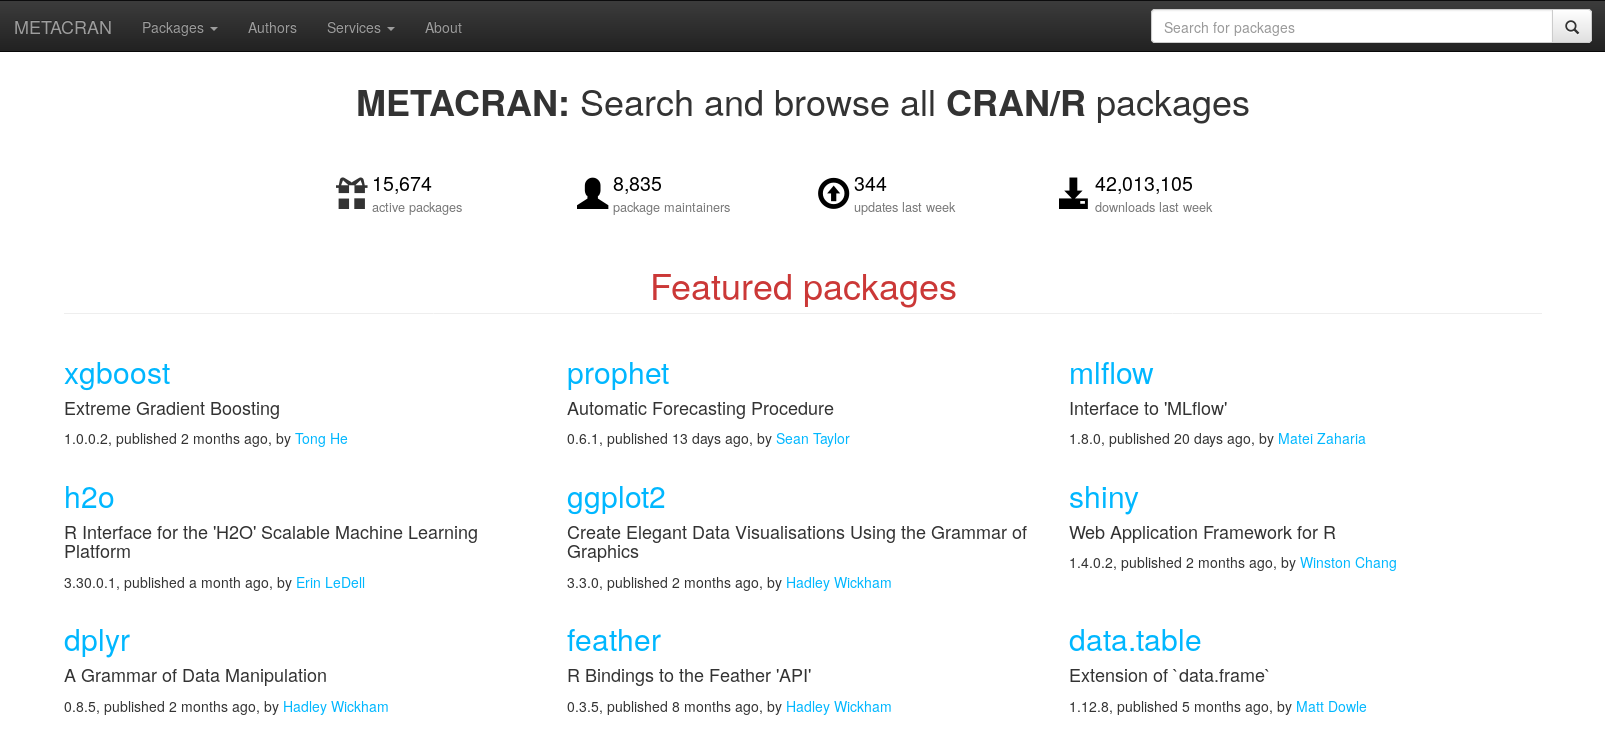
\includegraphics{img/chap2/metacran.png}
\caption{Haut de la page principale du \emph{METACRAN} \url{https://www.r-pkg.org/} consultée le}
\end{figure}

Combien de packages existent-t-il actuellement ? Dans le numéro de décembre 2009 du \emph{The R journal}, John Fox relate la croissance exponentielle du nombre de packages R \citep{fox_aspects_2009}. D'une centaine de packages au début des années 2000, on arrive à plus de 7000 en août 2015; la barre des 10000 packages a été franchie en 2017 et en février 2019, plus de 13600 packages sont disponibles sur le CRAN\footnote{Le nombre exact est indiqué en haut de la page \url{https://cran.r-project.org/web/packages/} consulté le 5 février.}.

\begin{figure}
\centering
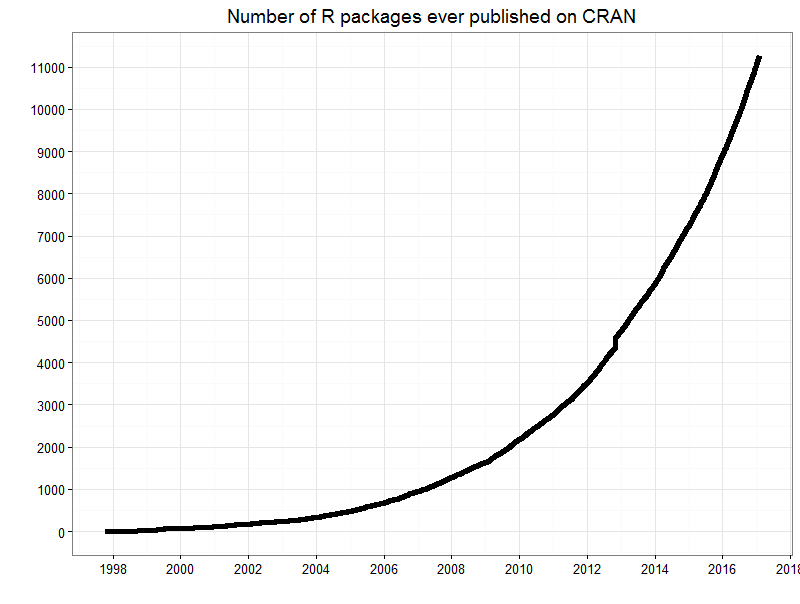
\includegraphics{img/chap2/package2017.png}
\caption{Croissance des packages R disponibles sur le CRAN - article de publié par David Smith sur le blog \emph{Revolutions} \url{https://blog.revolutionanalytics.com/2017/01/cran-10000.html}, consulté le 5 février 2019}
\end{figure}

À ce nombre de packages viennent s'ajouter près de 1700 packages disponibles sur \href{https://www.bioconductor.org/}{Bioconductor} et des dizaines de milliers disponibles
sur différentes forges logiciel : \href{https://r-forge.r-project.org/}{R-forge}, \href{http://www.omegahat.net/}{omegahat}, \href{https://github.com/}{GitHub}, \href{https://bitbucket.org/}{bitbucket}. Le site \href{https://rdrr.io/}{R Package Documentation} rassemble la documentation des packages disponibles sous différentes plateformes.

\begin{figure}
\centering
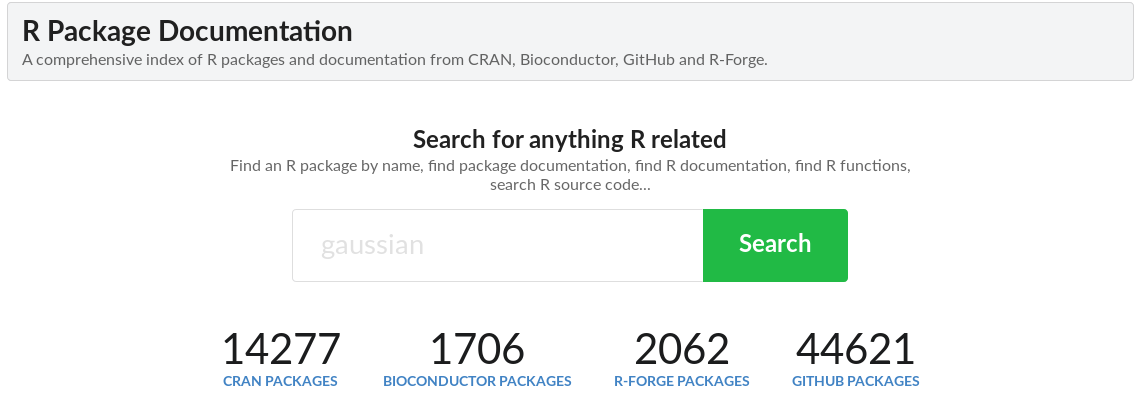
\includegraphics{img/chap2/rdrr.png}
\caption{Haut de la page principale du \emph{R Package Documentation} \url{https://rdrr.io/} consultée le 5 février 2019}
\end{figure}

Comme le soulignait déjà Kurt Hortnik en 2009 \citep{hornik_are_2012}, cette abondance de packages pose un certain nombre de questions relatives à la facilité de trouver la fonctionnalité désirée, la redondance des fonctions et la qualité du code. Les tests auxquels sont soumis les packages soumis au CRAN ne couvrent pas complètement ces deux derniers aspects. Selon Kurt Hortnik, en dépit des défis posés par le nombre croissant de packages développés, une politique plus contraignante n'est pas souhaitable, et quand bien même celle-ci serait mise en place, elle n'affecterait pas tant la courbe de croissance. À son avis, il faudrait repenser les relations entre les packages afin de diminuer la similarité entre les packages au profit d'interdépendances. Une première mesure pour maintenir une augmentation de la qualité des packages sur le CRAN est de permettre au utilisateur de donner un retour de leur utilisation (rapporté des bogues notamment). Les forges logiciel telles que \emph{Github}, \emph{Bitbucket} ou \emph{R-Forge} sont fait pour cela et leur utilisation est de plus en plus fréquente. Une autre mesure est d'inciter les créateurs de packages à faire évaluer leur travail par les pairs, en soumettant leur package à des journaux/organisations spécialisée comme \emph{Journal of Open Source Software} ou rOpenSci (voir plus haut).

\hypertarget{les-interfaces-utilisateurs}{%
\subsubsection{Les interfaces utilisateurs}\label{les-interfaces-utilisateurs}}

Travailler avec R, c'est écrire des lignes de code dans le langage R qui sont interprétées par R et pour cela, l'utilisateur utilise le programme R qui peut être ouvert de différentes manière. Par exemple en tapant \texttt{R} dans un émulateur de Terminal\footnote{\url{https://fr.wikipedia.org/wiki/\%C3\%89mulateur_de_terminal}, consulté le 6 Février 2019.}.

\begin{figure}
\centering
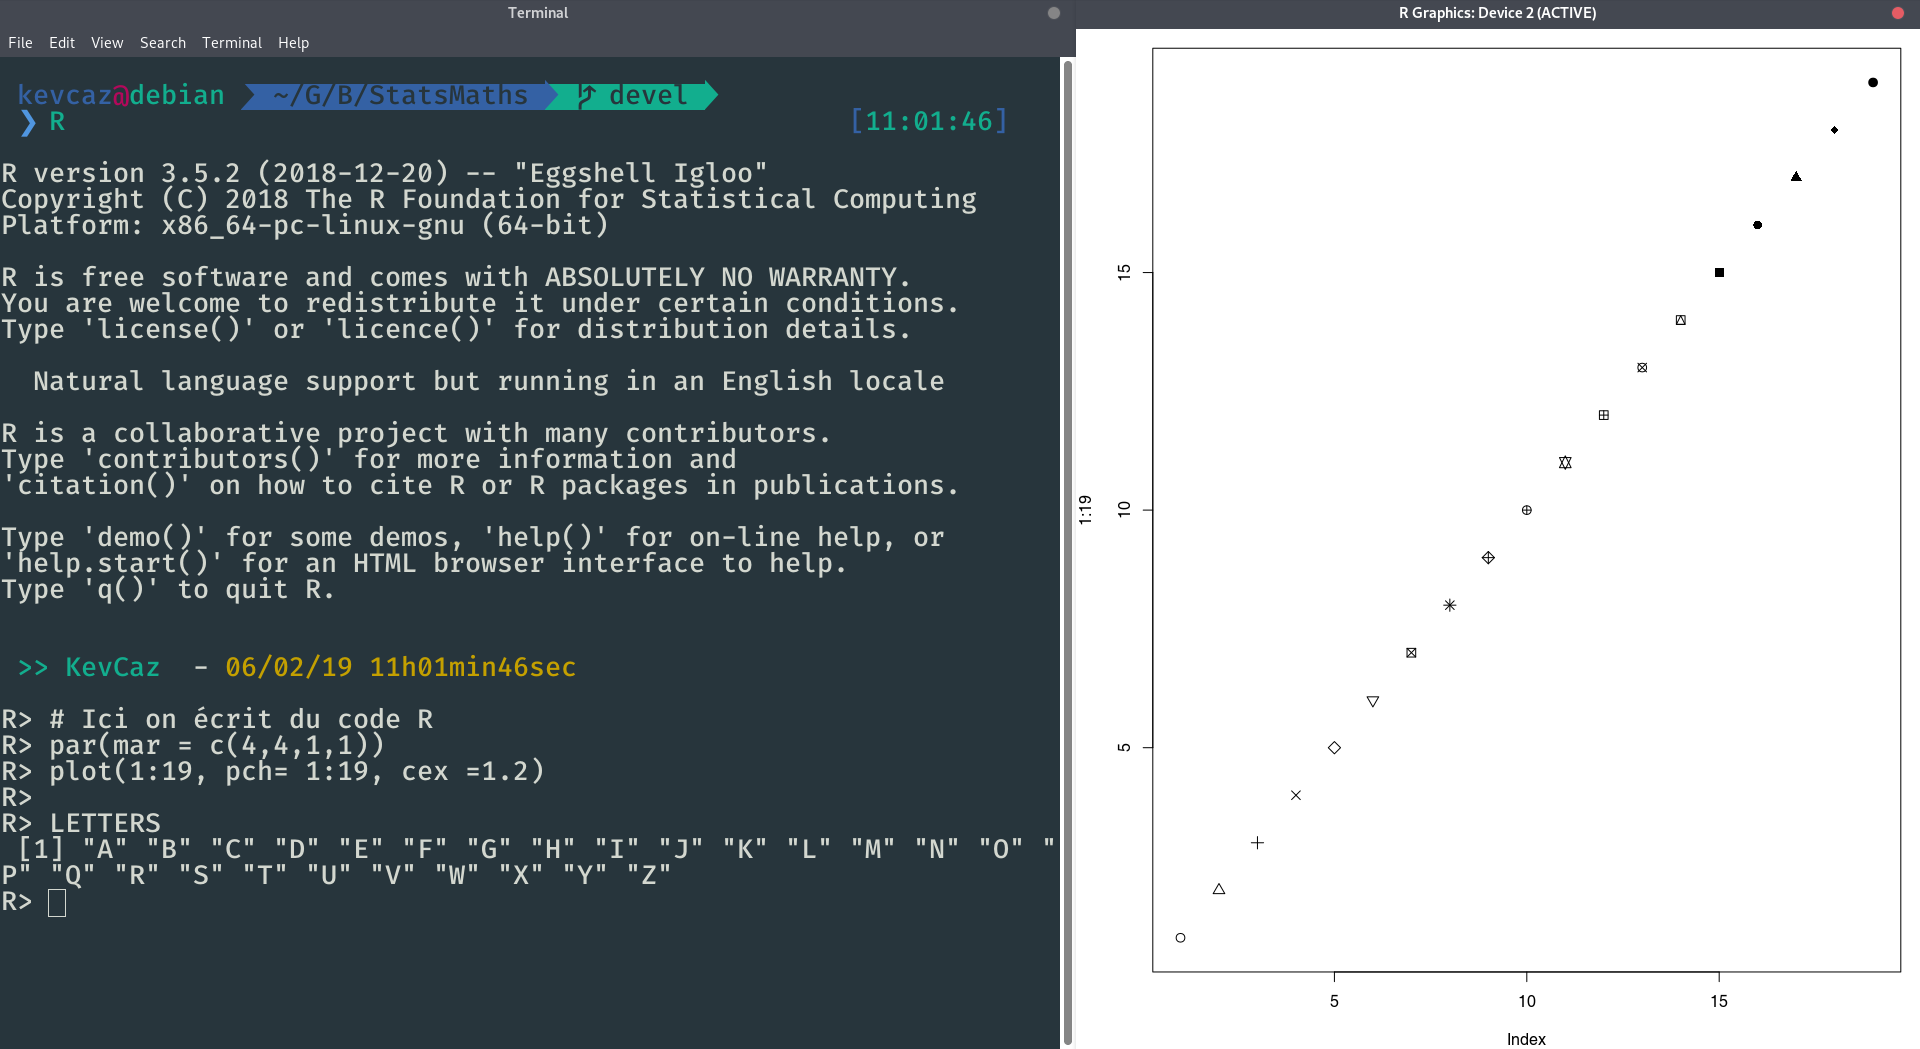
\includegraphics{img/chap2/terminal.png}
\caption{R lancé dans GNOME Terminal 3.30.2}
\end{figure}

À chaque utilisation de R, l'utilisateur écrit une suite plus ou moins longue de commandes et utiliser simplement la console pour travailler son code est finalement assez peu efficace. C'est pour cela qu'on a recourt à un éditeur de code avec lequel l'utilisateur crée des fichier \texttt{.R} dans lequel il rédige les suites de commandes qu'il envoie vers la console R. Donc, ce qu'il fait pour travailler efficacement avec R c'est une console R et un éditeur de code. Il existe des logiciels qui offrent les deux fonctionnalités. Par exemple, lorsque R est téléchargé depuis le CRAN, il est fournit avec une interface utilisateur assez minimaliste avec laquelle l'utilisateur peut facilement créer des scripts et et une console R est ouverte à l'ouverture du logiciel.

\begin{figure}
\centering
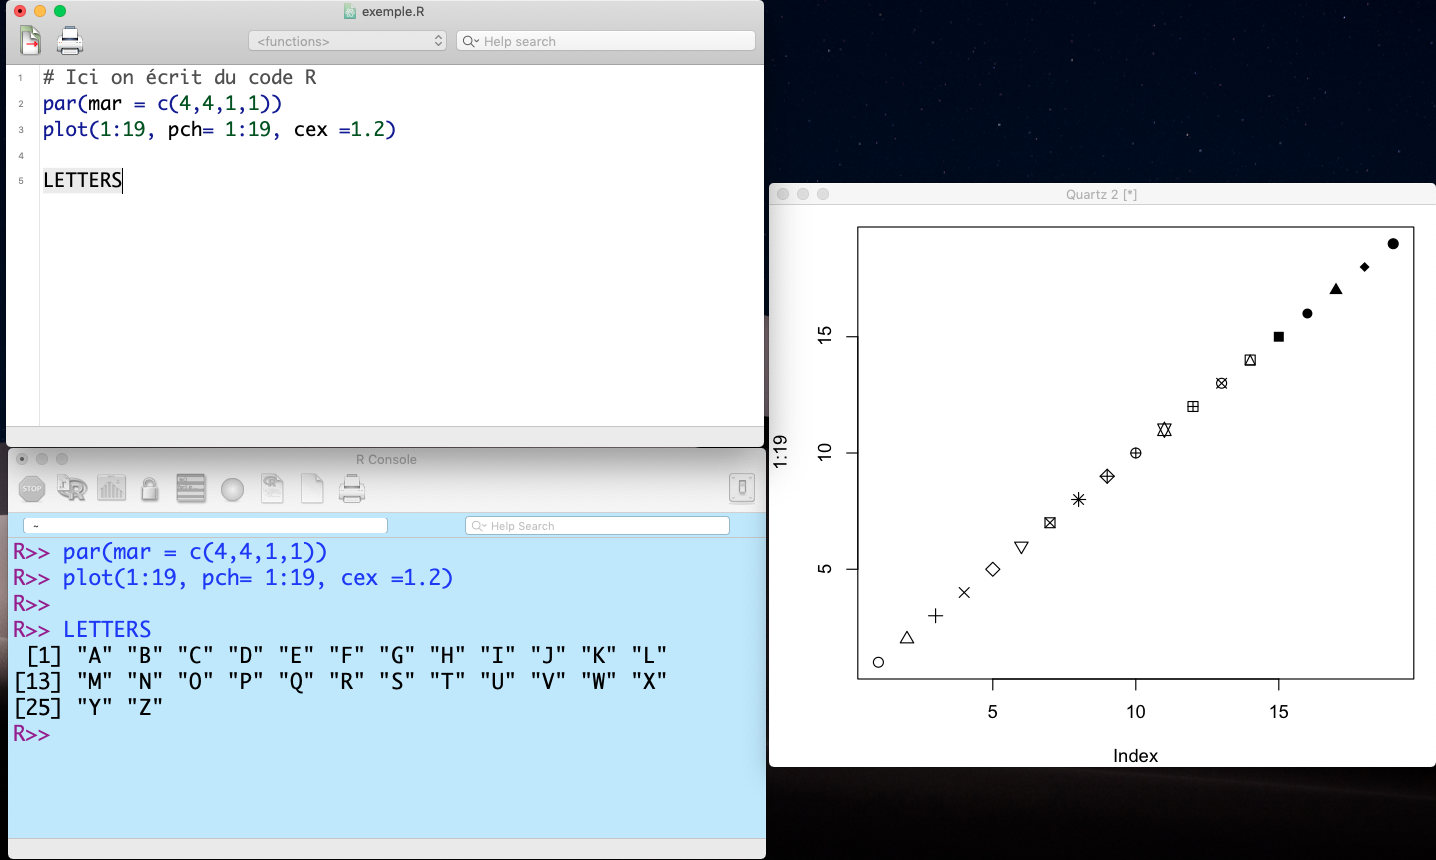
\includegraphics{img/chap2/rgui.png}
\caption{R utilisé avec l'interface utilisateur téléchargée depuis le CRAN}
\end{figure}

Comme nous l'avons mentionné précédemment, une des interfaces utilisateurs les plus utilisée actuellement est \href{https://www.rstudio.com}{RStudio}. RStudio est un logiciel multi-plateforme et gratuit (pour la version \emph{Desktop} qui nous intéresse ici) qui permet de visualiser facilement la console où le code est exécuté, l'éditeur de lignes de code, les figures réalisées, la liste des packages chargés, la documentation, etc. Cette interface est à recommander lorsqu'on débute avec R et pour la suite si vous utiliser principalement R.

\begin{figure}
\centering
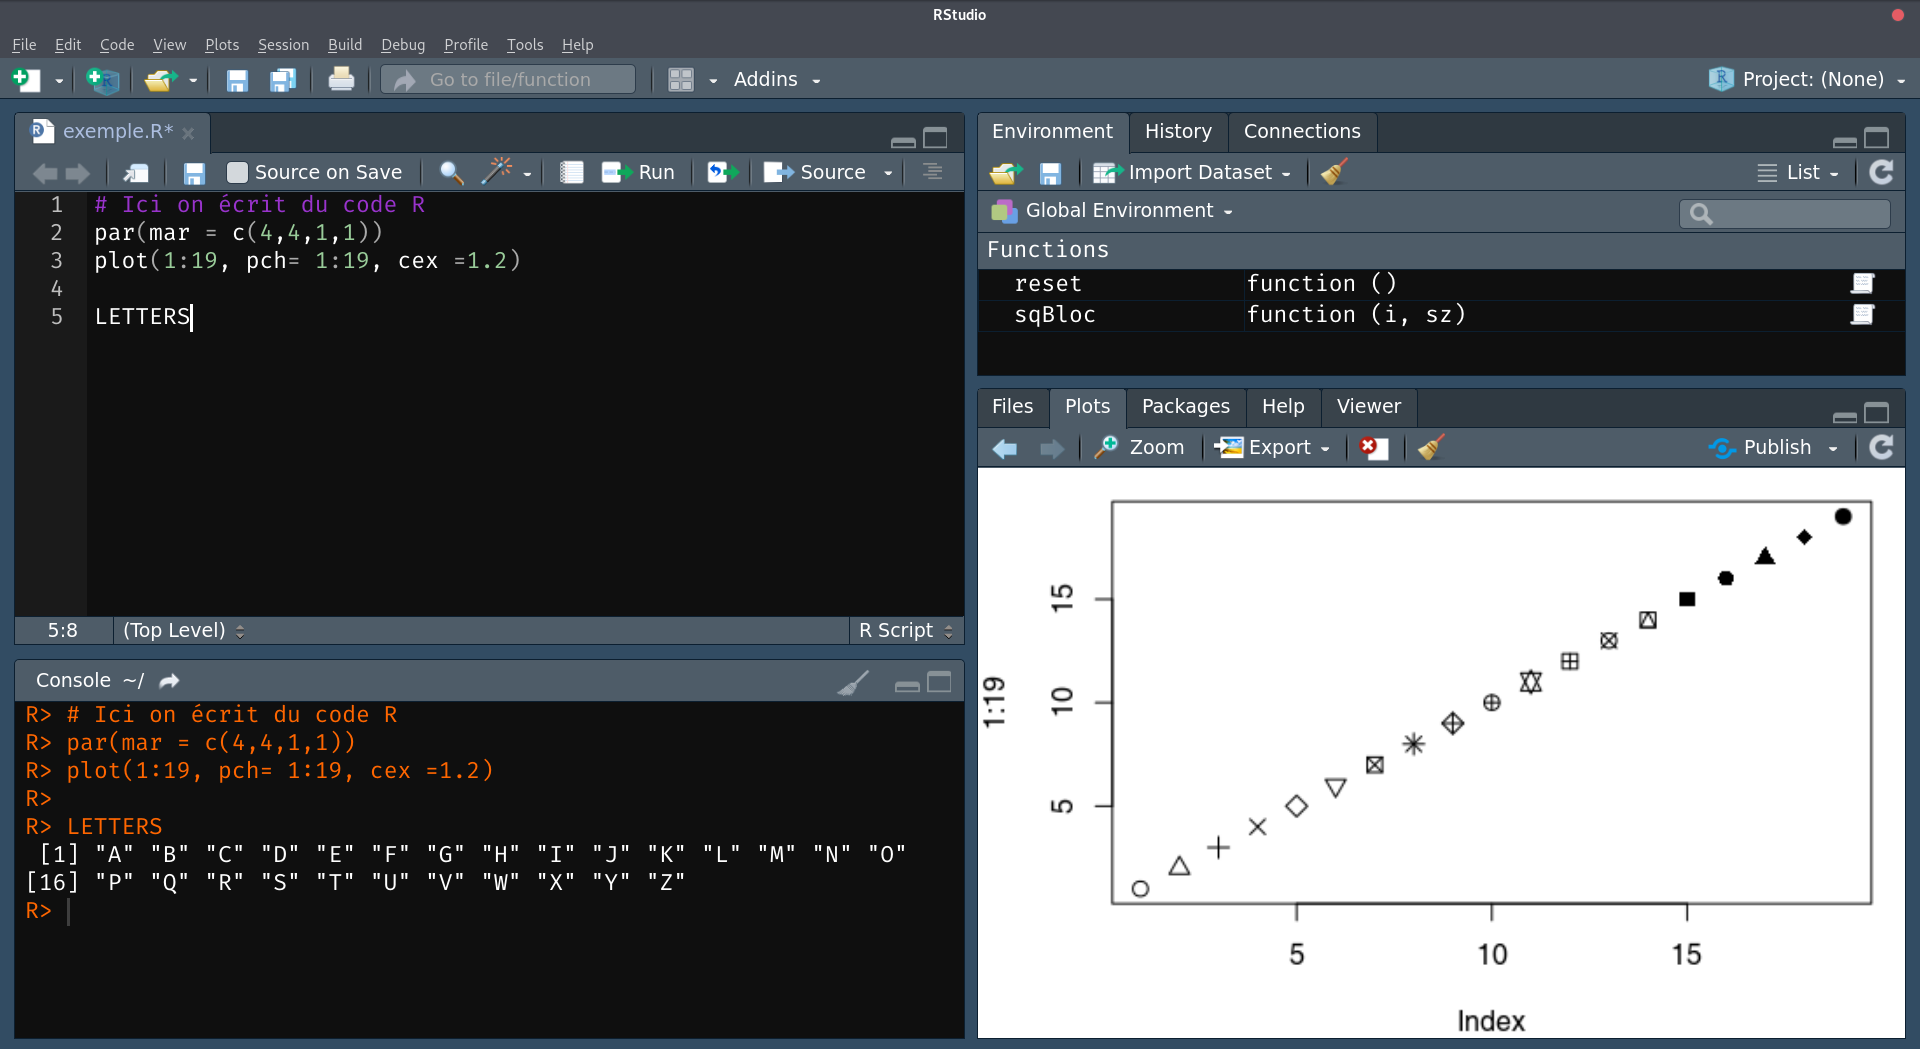
\includegraphics{img/chap2/rstudio.png}
\caption{RStudio}
\end{figure}

Enfin, il est aussi possible d'utiliser R avec des éditeurs de codes généralistes, citons en quelques uns:

\begin{itemize}
\tightlist
\item
  \href{https://www.gnu.org/software/emacs/}{Emacs}
\item
  \href{https://www.vim.org/}{Vim}
\item
  \href{https://code.visualstudio.com/}{Visual Studio Code}
\item
  \href{https://www.sublimetext.com/}{Sublime Text}
\item
  \href{https://atom.io/}{Atom}
\end{itemize}

Chacun des ces logiciels offrent de multiples fonctionnalités et viennent avec des extensions pratiques pour l'utilisation d'un très grande quantité de langages de programmation dont R. L'avantage de ces éditeurs de code est la multitude des fonctionnalités qui sont empruntées à différentes communautés de programmateurs. Avec ces logiciels, au prix de quelques heures de prise en main, il est possible d'avoir un environment de travail multi-langage, personnalisé d'une très grande efficacité.

\begin{figure}
\centering
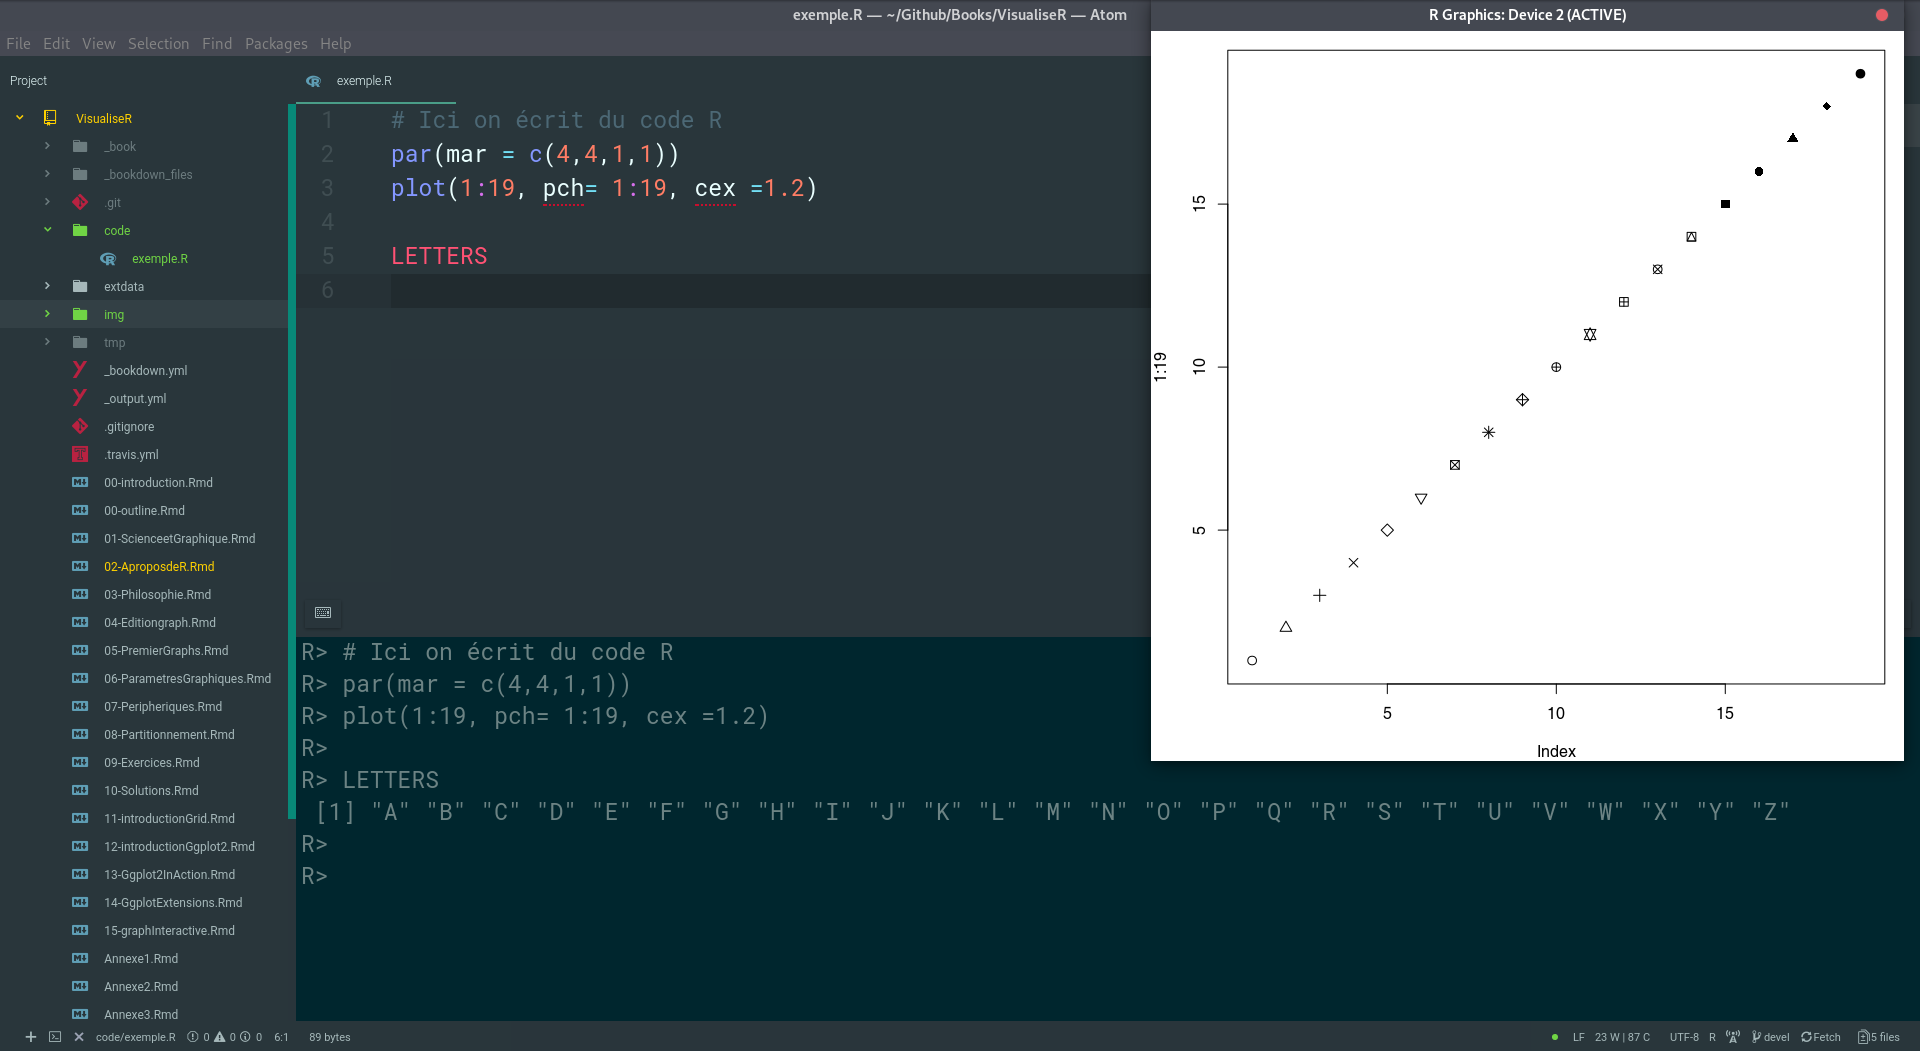
\includegraphics{img/chap2/ratom.png}
\caption{Utilisé R avec atom}
\end{figure}

Cette section donne un aperçu des possibilités qui existent pour travailler avec R. Si vous débutez avec R sans grande expérience en programmation, nous recommandons l'utilisation de R Studio. Si vous êtes un programmateur chevronné et que vous utilisez déjà un éditeur de code performant et généraliste, il est probable que vous trouverez des extensions pour R pour cet éditeur de code pour cet éditeur de code en particulier.

\hypertarget{les-diffuxe9rents-systuxe8mes-graphiques-dont-r-dispose}{%
\section{Les différents systèmes graphiques dont R dispose}\label{les-diffuxe9rents-systuxe8mes-graphiques-dont-r-dispose}}

R dispose de nombreux outils pour faire un travail approfondi de visualisation
des données. Lorsque R est installé, nous avons à notre disposition de multiple
fonctionnalités pour créer, éditer et exporter des figures.
L'édition de graphique sous R peut être divisé en trois branches : d'un côté
l'approche développée dans le package \emph{graphics}, celle du package \emph{grid} (qui inclus ggplot2) et une troisième, hétérogène, qui est l'ensemble des libraries qui utilisent d'autres languages, comme par exemple javascript, (et ainsi créer des figures dans un navigateur web).

\hypertarget{les-uxe9tapes-pour-cruxe9er-un-graphique-avec-r}{%
\subsection{Les étapes pour créer un graphique avec R}\label{les-uxe9tapes-pour-cruxe9er-un-graphique-avec-r}}

\hypertarget{le-systuxe8me-graphique-du-package-graphics}{%
\subsection{\texorpdfstring{Le système graphique du package \emph{graphics}}{Le système graphique du package graphics}}\label{le-systuxe8me-graphique-du-package-graphics}}

Le package \emph{graphics} est une implémentation du système graphique historique de
\emph{S}. Il s'agit, en effet, de la ré-écriture des fonctionnalités de la
bibliothèque GRZ pour les utiliser avec R. Ce travail a été en large partie mené
par Ross Ihaka, l'un des deux initiateurs de R. Avec ce package, nous pouvons
obtenir en très peu de lignes de commandes des graphiques tout à fait convenable
(grâce, par exemple, à la fonction \emph{plot()}). Nous pouvons également travailler
par couches successive pour ajouter un à un les éléments du graphiques et
obtenir un rendu graphique plus aboutit. l'utilisation de \emph{graphics} est
répandue, simple, intuitive et sa puissance est souvent mésestimée. C'est pour
ces raisons que nous avons choisi de la détailler dans ce livre. De manière
générale, pour faire un graphique avec ce système on procède en trois
étapes\&nbsp:

\begin{enumerate}
\def\labelenumi{\arabic{enumi}.}
\tightlist
\item
  On définit les paramètre graphiques globaux (fonction \emph{par()} voir chapitre)
\item
  On trace le plot ajoute la fonction que nous souhaitons (\emph{plot()}, \emph{boxplot()},\ldots{}.)
\item
  On ajoute les différents éléments supplémentaire : points, lignes, textes, légendes.
\end{enumerate}

Dans la suite, nous reprenons point par point ces différentes étapes. Une des
principales faiblesses de ce système réside dans la difficulté à changer les
éléments déjà placés. La plupart du temps, il est nécessaire de ré-exécuter tout
le code modifier. Ce système est riche en fonctionnalités et plusieurs package
de R utilise ce système pour implémenter des graphiques plus spécifiques. Le
package \emph{plotrix}, développé par Jim Lemon, utilise \emph{graphics} et ajoute à
celui-ci de nombreux types de graphiques supplémentaires dont les graphiques en
co-ordonnées polaires.

\hypertarget{le-systuxe8me-graphique-du-package-grid}{%
\subsection{\texorpdfstring{Le système graphique du package \emph{grid}}{Le système graphique du package grid}}\label{le-systuxe8me-graphique-du-package-grid}}

Le package \emph{grid}, que nous devons à Paul Murrel, est un système graphique puissant qui donne un cadre performant pour développer des graphiques précis. Il y a plusieurs éléments importants sur lesquels nous revenons en annexe. Le premier est le concept de \emph{viewPort} : il s'agit de zone rectangulaire qui sont définis dans l'espace et avec un système de co-ordonnées. Il est possible d'en utiliser autant que souhaité, elles peuvent se recouper ou non et posséder des paramètres. C'est en quelques sortes un ensemble très flexibles de calques. Il est possible de naviguer à travers pour placer à tout moment n'importe quel élément du future graphique. Le package \emph{grid} définis ces propres fonctions primitives pour dessiner points, lignes et polygones. En plus d'un affichage et contrairement à ce que nous avons dans le package \emph{graphics}, dans \emph{grid}, les objets affichés sont aussi des objets que l'on peut modifier à sa guise. Cela donne au package \emph{grid} une grande puissance. Il serait bien long de redévelopper chaque graphique avec grid et comparer \emph{graphics} et \emph{grid} est un peu bancal en se sens qu'il ne sont pas réellement implémenté et qu'il faut les faire à la main. Néanmoins c'est grâce à sa puissance que sont nés deux autres systèmes de graphique à succès. Le premier est le système développé par Deepayan Sarkar dans le package \emph{lattice}. Le second est une implémentation de la grammaire des graphiques de (voir la section précédente), \emph{ggplot2} que nous devons à Hadley Wickham. Notez que depuis peu, \emph{grid} et \emph{graphics} ont été reliés partiellement grâce au package \emph{gridGraphics} qui permet d'écrire les fonctions graphics en \emph{grid}.
Ces packages doivent beaucoup au travail de Paul Murrel dont le livre \emph{R graphics} {[}ref{]} et aussi un chapitre sur lattice demeure une référence pour approfondir l'édition de graphiques avec R.

Lorsque les graphiques sont produits que ce soit avec \emph{grid} ou \emph{graphics}, pour les exporter dans différent format, on fait appel à un troisième package : \emph{grDevices}.

\hypertarget{les-graphiques-interactives}{%
\subsection{Les graphiques interactives}\label{les-graphiques-interactives}}

Les graphiques qui font appel à des bibliothèques JS.

\hypertarget{interfaes}{%
\subsection{Interfaes}\label{interfaes}}

\hypertarget{part-utiliser-graphics}{%
\part{Utiliser graphics}\label{part-utiliser-graphics}}

\hypertarget{uxe9dition-dun-graphique}{%
\section{Édition d'un graphique}\label{uxe9dition-dun-graphique}}

\hypertarget{graphique-vierge}{%
\subsection{Graphique vierge}\label{graphique-vierge}}

La philosophie des auteurs en termes de graphiques sous R est simple : ajouter les éléments un à un, en commençant par ouvrir une fenêtre graphique avec des dimensions (axes et marges) choisies, mais sans que rien ne s'affiche à l'écran. Regardons donc comment créer un graphe vide.
Lorsqu'on fait appel à la fonction \texttt{plot()}, les axes sont déterminés automatiquement par R en fonction de l'étendue des valeurs des données que l'on souhaite représenter. Nous allons regarder comment modifier l'étendue des axes à l'aide de deux arguments : \texttt{xlim} et \texttt{ylim}.
Créons tout d'abord deux variables continues.

\begin{Shaded}
\begin{Highlighting}[]
\NormalTok{(x1 <-}\StringTok{ }\KeywordTok{sample}\NormalTok{(}\DataTypeTok{x =} \DecValTok{0}\OperatorTok{:}\DecValTok{10}\NormalTok{, }\DataTypeTok{size =} \DecValTok{20}\NormalTok{, }\DataTypeTok{replace =} \OtherTok{TRUE}\NormalTok{))}
\CommentTok{#>  [1]  4  5  1  1  0  8  4  3  7  6  2  9 10  9  4  9  4  2  8  4}
\NormalTok{(x2 <-}\StringTok{ }\KeywordTok{sample}\NormalTok{(}\DataTypeTok{x =} \DecValTok{10}\OperatorTok{:}\DecValTok{20}\NormalTok{, }\DataTypeTok{size =} \DecValTok{20}\NormalTok{, }\DataTypeTok{replace =} \OtherTok{TRUE}\NormalTok{))}
\CommentTok{#>  [1] 12 19 11 19 12 20 15 20 13 16 10 14 17 11 20 18 14 13 12 16}
\end{Highlighting}
\end{Shaded}

Ces deux variables ne varient pas de la même manière. Nous allons faire deux graphes. Le premier utilisera les paramètres par défaut de R. Dans le second, nous allons fixer les axes de manière à ce qu'ils soient bornés entre 0 et 20.

\begin{Shaded}
\begin{Highlighting}[]
\KeywordTok{par}\NormalTok{(}\DataTypeTok{mfrow =} \KeywordTok{c}\NormalTok{(}\DecValTok{1}\NormalTok{, }\DecValTok{2}\NormalTok{))}
\KeywordTok{plot}\NormalTok{(x1, x2)}
\KeywordTok{plot}\NormalTok{(x1, x2, }\DataTypeTok{xlim =} \KeywordTok{c}\NormalTok{(}\DecValTok{0}\NormalTok{, }\DecValTok{20}\NormalTok{), }\DataTypeTok{ylim =} \KeywordTok{c}\NormalTok{(}\DecValTok{0}\NormalTok{, }\DecValTok{20}\NormalTok{))}
\end{Highlighting}
\end{Shaded}

\begin{center}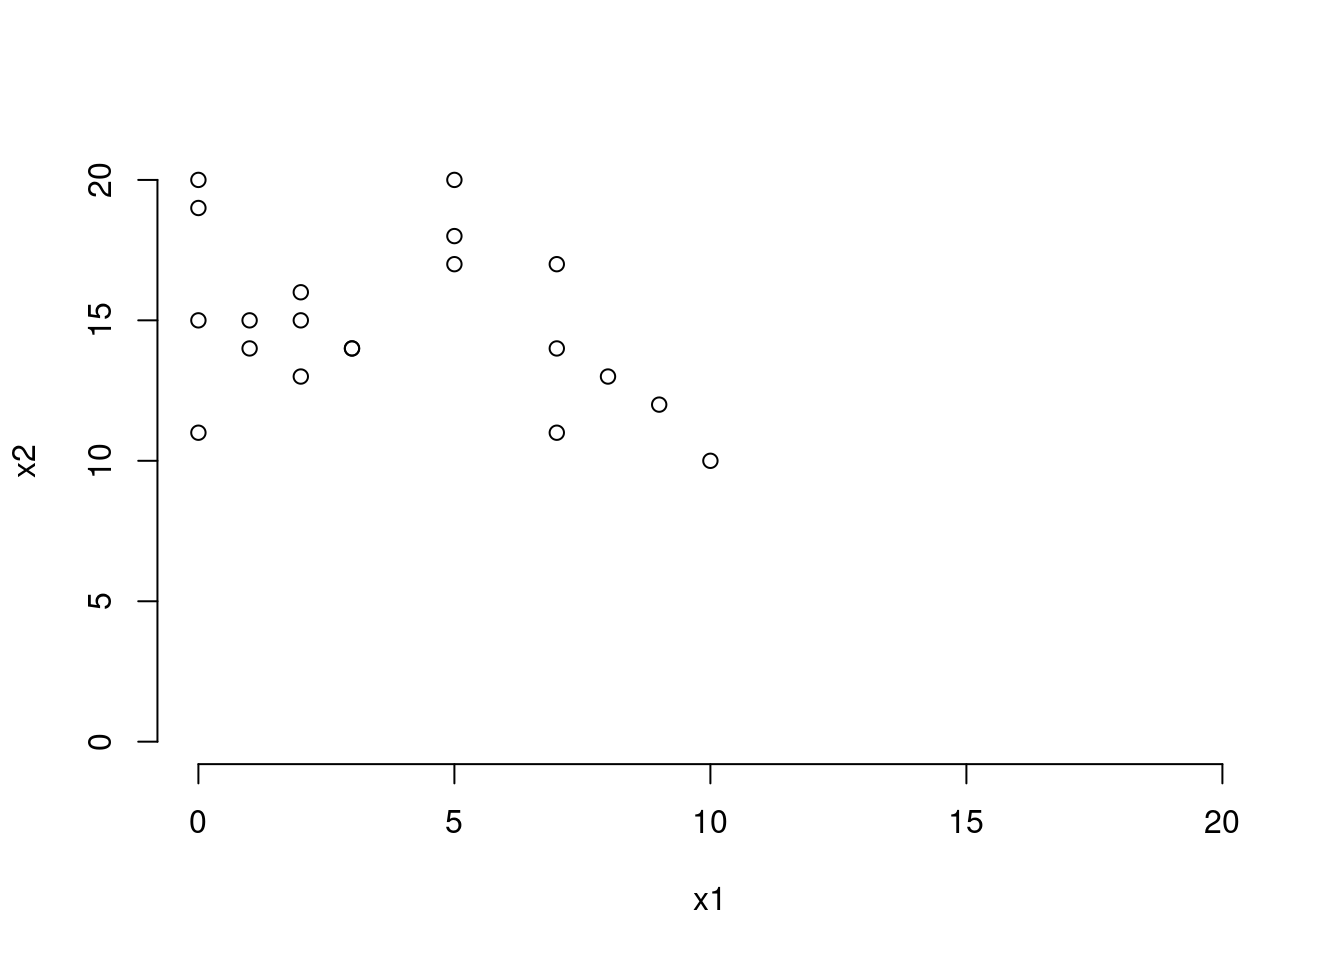
\includegraphics{visualiseR_files/figure-latex/unnamed-chunk-3-1} \end{center}

Par défaut, la fonction \texttt{plot()} affiche une boîte autour de la région graphique. C'est l'argument \texttt{bty} qui défini cela. Par défaut, il prend la valeur \textbf{``o''}. Pour supprimer ce cadre, on peut lui attribuer la valeur \textbf{``n''}.

\begin{Shaded}
\begin{Highlighting}[]
\KeywordTok{plot}\NormalTok{(x1, x2, }\DataTypeTok{xlim =} \KeywordTok{c}\NormalTok{(}\DecValTok{0}\NormalTok{, }\DecValTok{20}\NormalTok{), }\DataTypeTok{ylim =} \KeywordTok{c}\NormalTok{(}\DecValTok{0}\NormalTok{, }\DecValTok{20}\NormalTok{), }\DataTypeTok{bty =} \StringTok{"n"}\NormalTok{)}
\end{Highlighting}
\end{Shaded}

\begin{center}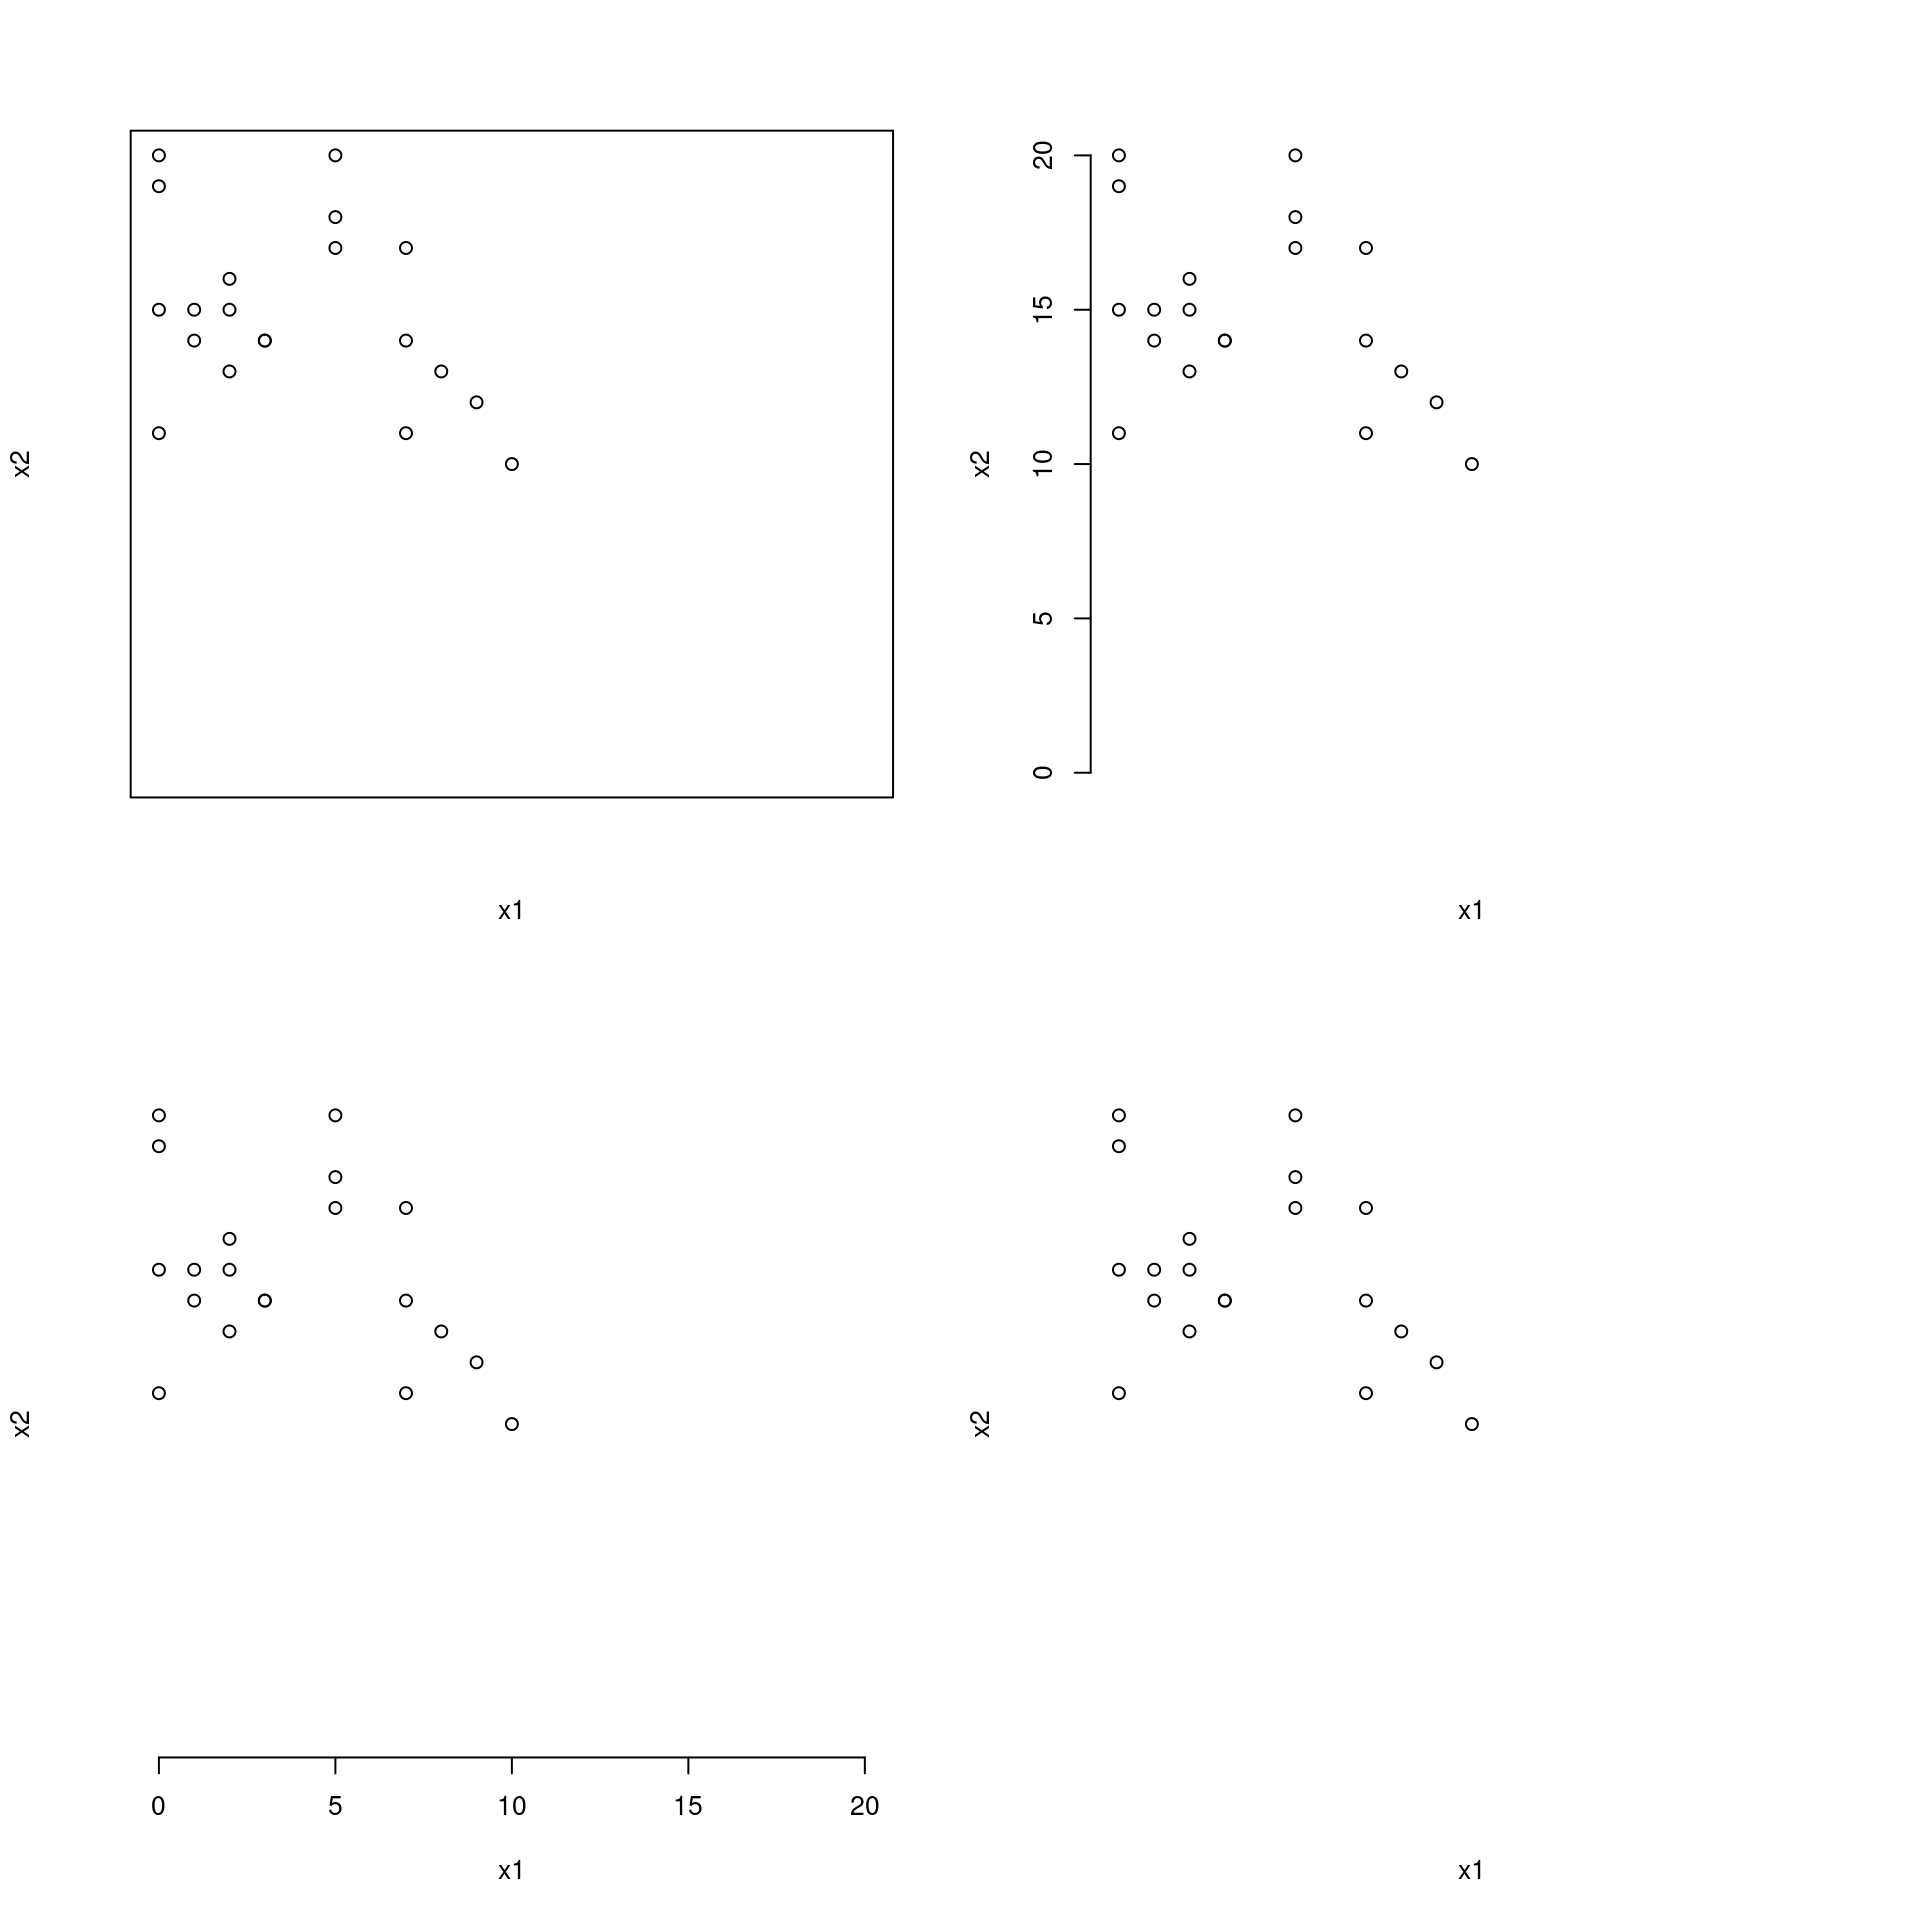
\includegraphics[width=.55\linewidth]{visualiseR_files/figure-latex/unnamed-chunk-4-1} \end{center}

Maintenant que nous avons fixé les axes, nous allons les supprimer. Ceci n'aura aucune incidence sur l'étendue du graphe. Pour ce faire, nous allons utiliser les arguments \texttt{xaxt} et \texttt{yaxt} qui contrôlent l'affichage des axes. L'argument \texttt{axes} permet quant à lui de supprimer à la fois les axes, mais aussi le cadre. Comparez ces graphes suivants

\begin{Shaded}
\begin{Highlighting}[]
\KeywordTok{par}\NormalTok{(}\DataTypeTok{mfrow =} \KeywordTok{c}\NormalTok{(}\DecValTok{2}\NormalTok{, }\DecValTok{2}\NormalTok{))}
\KeywordTok{plot}\NormalTok{(x1, x2, }\DataTypeTok{xlim =} \KeywordTok{c}\NormalTok{(}\DecValTok{0}\NormalTok{, }\DecValTok{20}\NormalTok{), }\DataTypeTok{ylim =} \KeywordTok{c}\NormalTok{(}\DecValTok{0}\NormalTok{, }\DecValTok{20}\NormalTok{), }\DataTypeTok{xaxt =} \StringTok{"n"}\NormalTok{, }\DataTypeTok{yaxt =} \StringTok{"n"}\NormalTok{)}
\KeywordTok{plot}\NormalTok{(x1, x2, }\DataTypeTok{xlim =} \KeywordTok{c}\NormalTok{(}\DecValTok{0}\NormalTok{, }\DecValTok{20}\NormalTok{), }\DataTypeTok{ylim =} \KeywordTok{c}\NormalTok{(}\DecValTok{0}\NormalTok{, }\DecValTok{20}\NormalTok{), }\DataTypeTok{bty =} \StringTok{"n"}\NormalTok{, }\DataTypeTok{xaxt =} \StringTok{"n"}\NormalTok{)}
\KeywordTok{plot}\NormalTok{(x1, x2, }\DataTypeTok{xlim =} \KeywordTok{c}\NormalTok{(}\DecValTok{0}\NormalTok{, }\DecValTok{20}\NormalTok{), }\DataTypeTok{ylim =} \KeywordTok{c}\NormalTok{(}\DecValTok{0}\NormalTok{, }\DecValTok{20}\NormalTok{), }\DataTypeTok{bty =} \StringTok{"n"}\NormalTok{, }\DataTypeTok{yaxt =} \StringTok{"n"}\NormalTok{)}
\KeywordTok{plot}\NormalTok{(x1, x2, }\DataTypeTok{xlim =} \KeywordTok{c}\NormalTok{(}\DecValTok{0}\NormalTok{, }\DecValTok{20}\NormalTok{), }\DataTypeTok{ylim =} \KeywordTok{c}\NormalTok{(}\DecValTok{0}\NormalTok{, }\DecValTok{20}\NormalTok{), }\DataTypeTok{axes =} \OtherTok{FALSE}\NormalTok{)}
\end{Highlighting}
\end{Shaded}

\begin{center}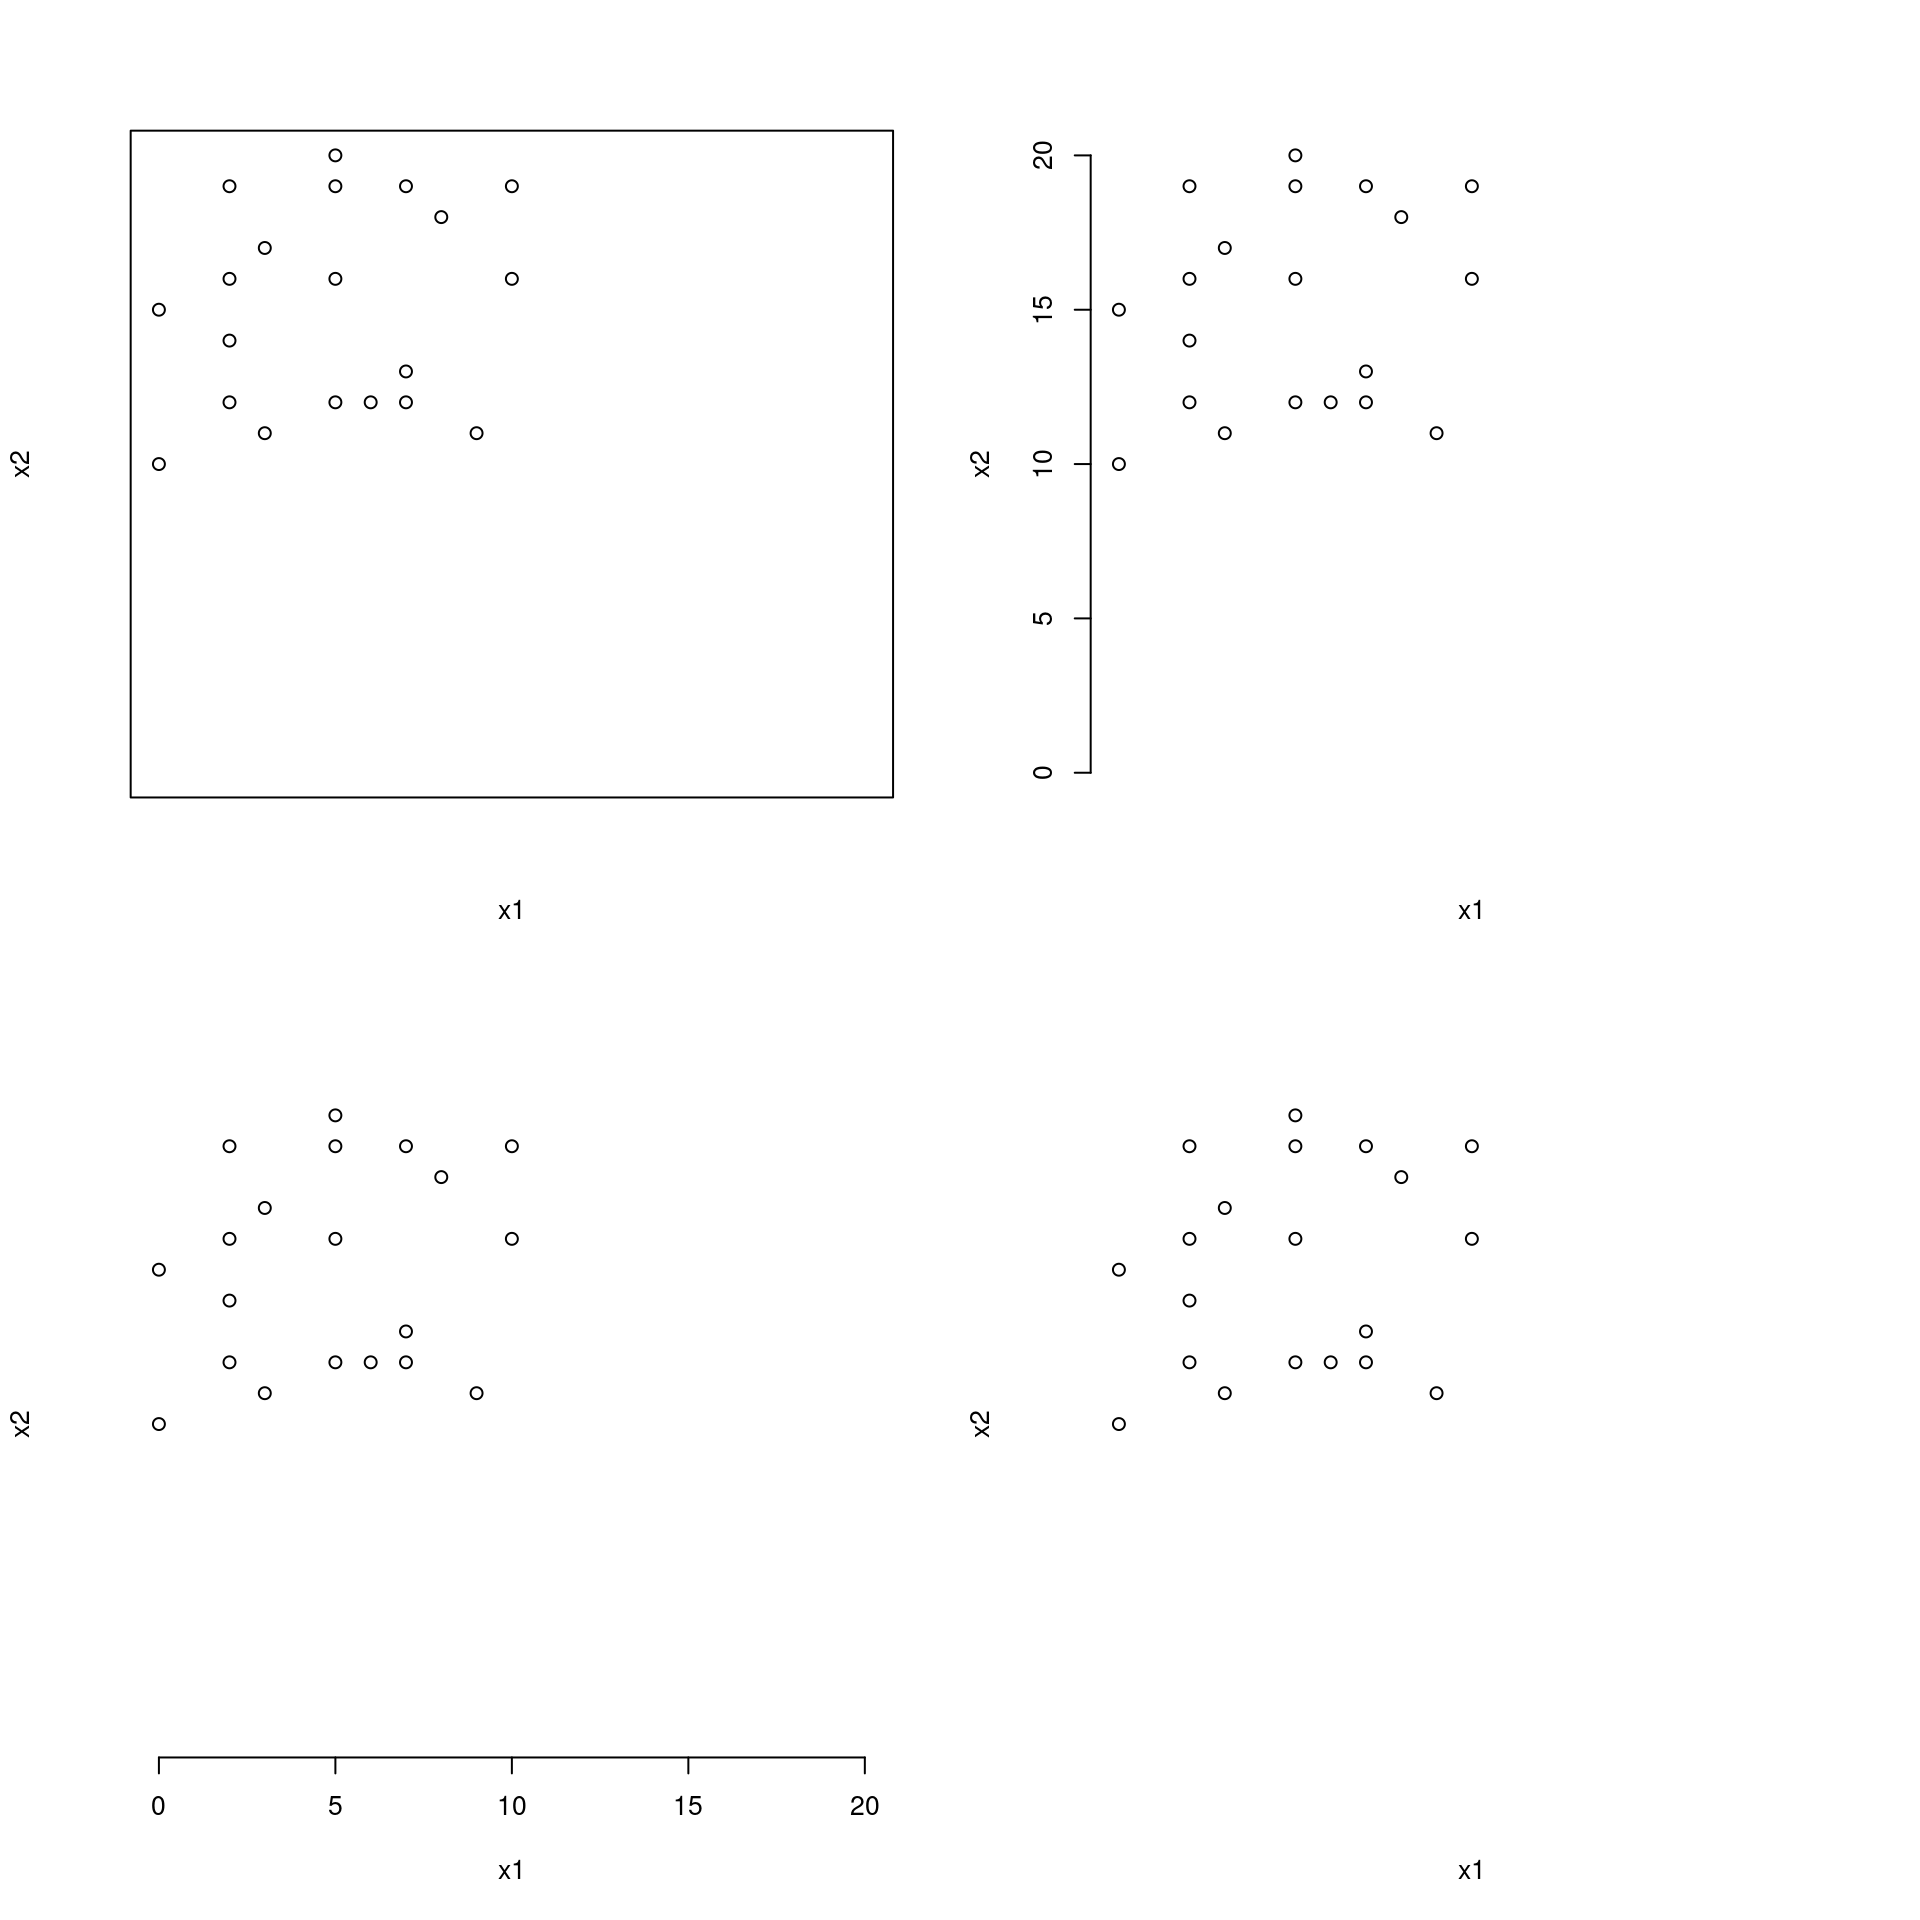
\includegraphics[width=1\linewidth]{visualiseR_files/figure-latex/unnamed-chunk-5-1} \end{center}

Poursuivons notre destruction graphique, et supprimons le nom des axes avec les arguments \texttt{xlab} et \texttt{ylab}. Par défaut, le nom des axes correspond au nom des variables. L'astuce ici consiste à leur attribuer la valeur \texttt{""}. Cependant, une alternative consisterait à utiliser l'argument \texttt{ann} qui va supprimer toute annotation dans le graphe (nom des axes, mais aussi titre et sous-titre).

\begin{Shaded}
\begin{Highlighting}[]
\KeywordTok{plot}\NormalTok{(x1, x2, }\DataTypeTok{xlim =} \KeywordTok{c}\NormalTok{(}\DecValTok{0}\NormalTok{, }\DecValTok{20}\NormalTok{), }\DataTypeTok{ylim =} \KeywordTok{c}\NormalTok{(}\DecValTok{0}\NormalTok{, }\DecValTok{20}\NormalTok{), }\DataTypeTok{axes =} \OtherTok{FALSE}\NormalTok{, }\DataTypeTok{ann =} \OtherTok{FALSE}\NormalTok{)}
\end{Highlighting}
\end{Shaded}

\begin{center}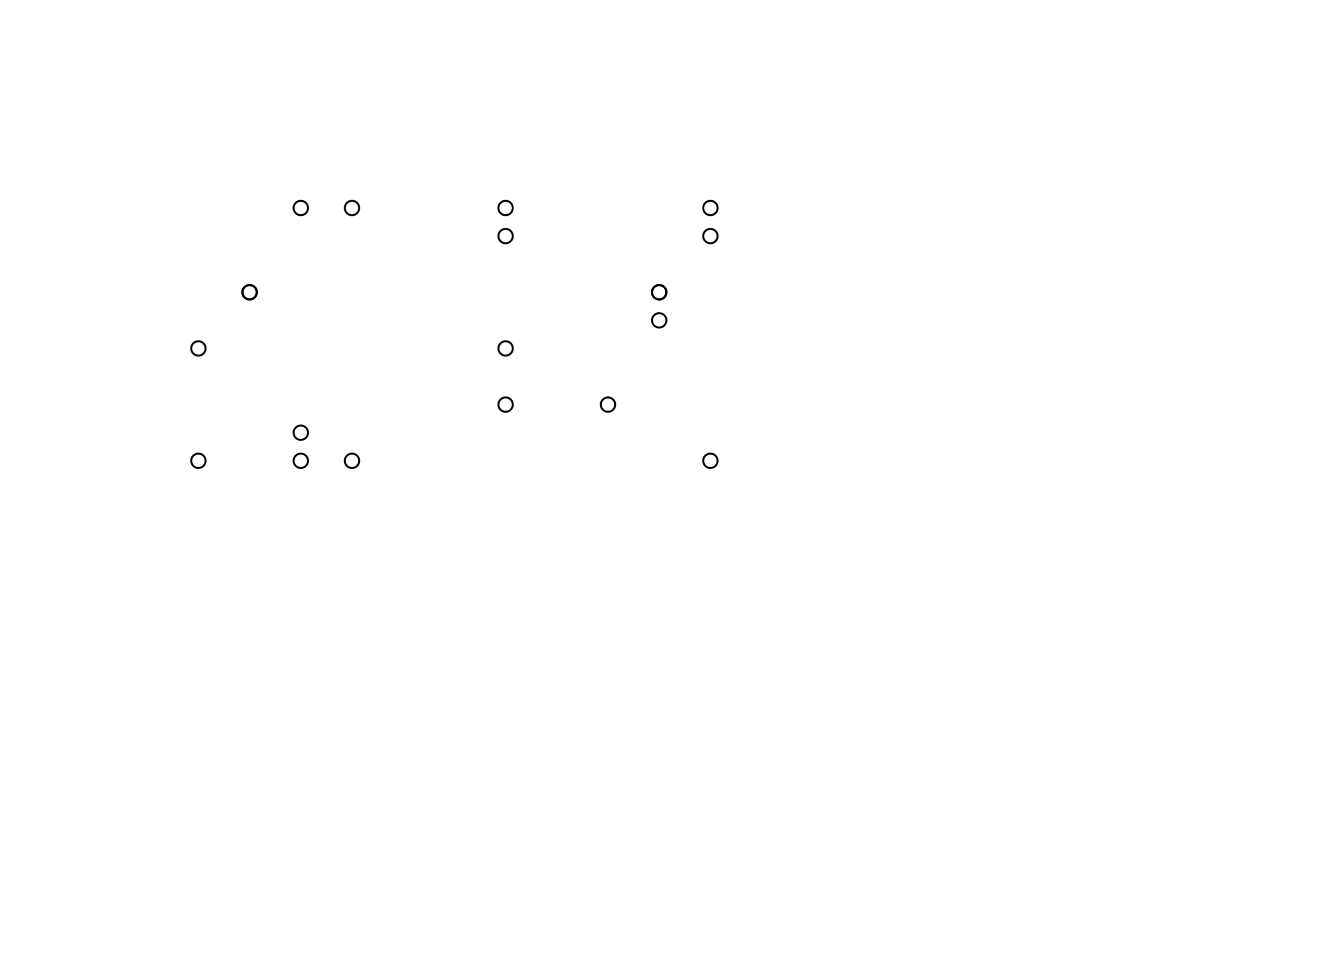
\includegraphics[width=.5\linewidth]{visualiseR_files/figure-latex/unnamed-chunk-6-1} \end{center}

Il ne nous reste plus qu'à supprimer les points avec l'argument \texttt{type}. Nous allons tout de même laisser le cadre afin de délimiter notre graphe.

\begin{Shaded}
\begin{Highlighting}[]
\KeywordTok{plot}\NormalTok{(x1, x2, }\DataTypeTok{xlim =} \KeywordTok{c}\NormalTok{(}\DecValTok{0}\NormalTok{, }\DecValTok{20}\NormalTok{), }\DataTypeTok{ylim =} \KeywordTok{c}\NormalTok{(}\DecValTok{0}\NormalTok{, }\DecValTok{20}\NormalTok{), }\DataTypeTok{xaxt =} \StringTok{"n"}\NormalTok{, }\DataTypeTok{yaxt =} \StringTok{"n"}\NormalTok{, }\DataTypeTok{ann =} \OtherTok{FALSE}\NormalTok{, }\DataTypeTok{type =} \StringTok{"n"}\NormalTok{)}
\end{Highlighting}
\end{Shaded}

\begin{center}
\includegraphics[width=.5\linewidth]{visualiseR_files/figure-latex/unnamed-chunk-7-1} \end{center}

Étant donné que nous fixons les bornes des axes, et que nous supprimons l'affichage des données, nous pourrions éviter de spécifier les données en x et en y, et simplement demander de (ne pas) représenter la valeur \textbf{0} (ou autre chose). Ainsi, l'écriture précédente pourrait se résumer à ceci (sans le cadre) :

\begin{Shaded}
\begin{Highlighting}[]
\KeywordTok{plot}\NormalTok{(}\DecValTok{0}\NormalTok{, }\DataTypeTok{xlim =} \KeywordTok{c}\NormalTok{(}\DecValTok{0}\NormalTok{, }\DecValTok{20}\NormalTok{), }\DataTypeTok{ylim =} \KeywordTok{c}\NormalTok{(}\DecValTok{0}\NormalTok{, }\DecValTok{20}\NormalTok{), }\DataTypeTok{axes =} \OtherTok{FALSE}\NormalTok{, }\DataTypeTok{ann =} \OtherTok{FALSE}\NormalTok{, }\DataTypeTok{type =} \StringTok{"n"}\NormalTok{)}
\end{Highlighting}
\end{Shaded}

Une particularité des programmeurs, c'est qu'il sont fainéants et s'ils peuvent économiser des lignes de code, alors ils le feront. Ainsi, nous allons créer une fonction qui implémentera un graphe vierge.

\begin{Shaded}
\begin{Highlighting}[]
\NormalTok{plot0 <-}\StringTok{ }\ControlFlowTok{function}\NormalTok{(}\DataTypeTok{y =} \DecValTok{0}\NormalTok{, }\DataTypeTok{x =}\NormalTok{ y, }\DataTypeTok{type =} \StringTok{"n"}\NormalTok{, }\DataTypeTok{axes =} \OtherTok{FALSE}\NormalTok{, }\DataTypeTok{ann =} \OtherTok{FALSE}\NormalTok{, ...)\{}
\KeywordTok{plot}\NormalTok{(x, y, }\DataTypeTok{axes =}\NormalTok{ axes, }\DataTypeTok{type =}\NormalTok{ type, }\DataTypeTok{ann =}\NormalTok{ ann, ...)}
\NormalTok{\}}
\end{Highlighting}
\end{Shaded}

Par la suite, il suffira de faire appel à cette fonction pour ouvrir un nouveau périphérique graphique n'affichant rien, mais dont les dimensions auront été spécifiées.

\begin{Shaded}
\begin{Highlighting}[]
\KeywordTok{plot0}\NormalTok{(}\DataTypeTok{xlim =} \KeywordTok{c}\NormalTok{(}\DecValTok{0}\NormalTok{, }\DecValTok{20}\NormalTok{), }\DataTypeTok{ylim =} \KeywordTok{c}\NormalTok{(}\DecValTok{0}\NormalTok{, }\DecValTok{20}\NormalTok{))}
\KeywordTok{box}\NormalTok{(}\StringTok{"plot"}\NormalTok{)}
\end{Highlighting}
\end{Shaded}

\begin{center}
\includegraphics[width=.5\linewidth]{visualiseR_files/figure-latex/unnamed-chunk-10-1} \end{center}

Remarque : la fonction \texttt{box} permet d'afficher un cadre autour de la région du plot (\texttt{"plot"}) ou de la figure (\texttt{"figure"}). Autre remarque : on pourrait utiliser cette fonction comme la fonction \texttt{plot()} et afficher, par ex. les données en indiquant \texttt{type\ =\ "p"}.

\hypertarget{ajout-de-points}{%
\subsection{Ajout de points}\label{ajout-de-points}}

Pour insérer des points sur un graphe, rien de plus simple : il suffit d'utiliser la fonction \texttt{points()}. Celle-ci partage un très grand nombre d'arguments avec la fonction \texttt{plot()}.
Créons trois nouvelles variables.

\begin{Shaded}
\begin{Highlighting}[]
\NormalTok{var1 <-}\StringTok{ }\KeywordTok{seq}\NormalTok{(}\DecValTok{1}\NormalTok{, }\DecValTok{20}\NormalTok{)}
\NormalTok{var2 <-}\StringTok{ }\KeywordTok{sample}\NormalTok{(var1, }\DecValTok{20}\NormalTok{, }\DataTypeTok{replace =} \OtherTok{FALSE}\NormalTok{)}
\NormalTok{var3 <-}\StringTok{ }\KeywordTok{sample}\NormalTok{(var1, }\DecValTok{20}\NormalTok{, }\DataTypeTok{replace =} \OtherTok{FALSE}\NormalTok{)}
\end{Highlighting}
\end{Shaded}

Nous allons maintenant représenter sur le même graphe \textbf{var2} en fonction de \textbf{var1}, puis dans un second temps \textbf{var3} en fonction de \textbf{var1}. Nous alloir voir trois exemples pour distinguer les deux séries de valeurs.

\begin{Shaded}
\begin{Highlighting}[]
\KeywordTok{par}\NormalTok{(}\DataTypeTok{mfrow =} \KeywordTok{c}\NormalTok{(}\DecValTok{2}\NormalTok{, }\DecValTok{2}\NormalTok{))}
\KeywordTok{plot}\NormalTok{(var1, var2, }\DataTypeTok{col =} \StringTok{"blue"}\NormalTok{, }\DataTypeTok{main =} \StringTok{"Couleurs"}\NormalTok{)}
\KeywordTok{points}\NormalTok{(var1, var3, }\DataTypeTok{col =} \StringTok{"red"}\NormalTok{)}
\KeywordTok{plot}\NormalTok{(var1, var2, }\DataTypeTok{pch =} \DecValTok{17}\NormalTok{, }\DataTypeTok{main =} \StringTok{"Symboles"}\NormalTok{)}
\KeywordTok{points}\NormalTok{(var1, var3, }\DataTypeTok{pch =} \DecValTok{15}\NormalTok{)}
\KeywordTok{plot}\NormalTok{(var1, var2, }\DataTypeTok{cex =} \DecValTok{1}\NormalTok{, }\DataTypeTok{main =} \StringTok{"Tailles"}\NormalTok{)}
\KeywordTok{points}\NormalTok{(var1, var3, }\DataTypeTok{cex =} \DecValTok{2}\NormalTok{)}
\end{Highlighting}
\end{Shaded}

\begin{center}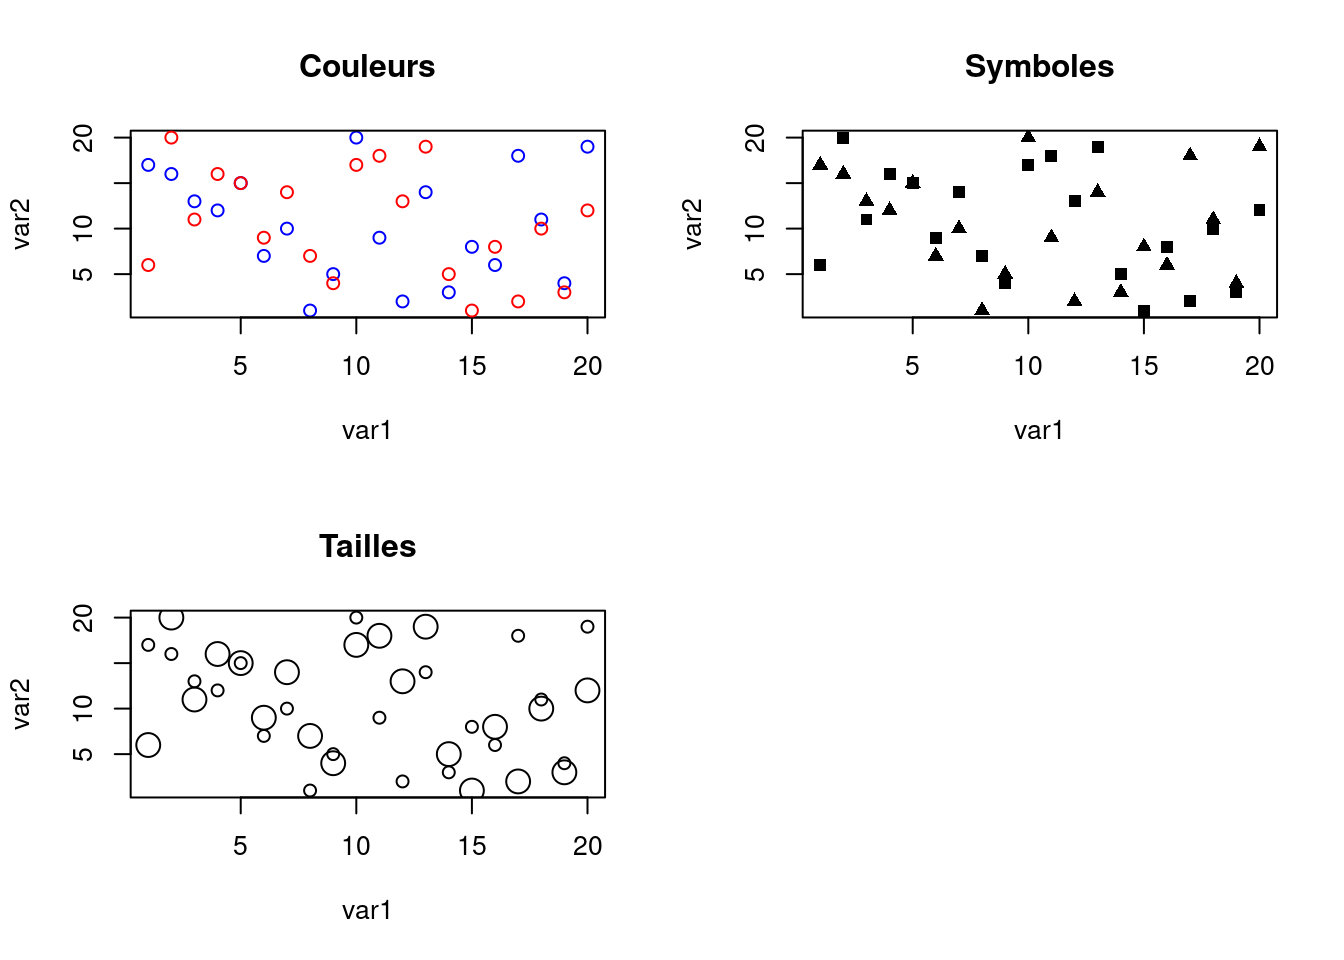
\includegraphics[width=.9\linewidth]{visualiseR_files/figure-latex/unnamed-chunk-12-1} \end{center}

Dans ces exemples, les trois variables présentaient la même gamme de valeurs (de 1 à 20). Si vous souhaitez superposer sur un même graphe des séries de points qui n'ont pas la même étendue de valeurs, il faudra convenablement définir les bornes des axes dans la fonction \texttt{plot()} avec les arguments \texttt{xlim} et \texttt{ylim} de manière à ce que toutes les séries de points s'affichent correctement.
Introduisons maintenant une commande intéressante sous R : la fonction \texttt{locator()}. Celle-ci permet de récupérer les coordonnées d'un (ou de plusieurs) clic(s) sur un graphique. Voici comment l'utiliser pour deux clics :

\begin{Shaded}
\begin{Highlighting}[]
\KeywordTok{locator}\NormalTok{(}\DataTypeTok{n =} \DecValTok{2}\NormalTok{)}
\end{Highlighting}
\end{Shaded}

Cette fonction permet également de rajouter simultanément des points sur le graphe au fur et à mesure des clics.

\begin{Shaded}
\begin{Highlighting}[]
\KeywordTok{locator}\NormalTok{(}\DataTypeTok{n =} \DecValTok{3}\NormalTok{, }\DataTypeTok{type =} \StringTok{"p"}\NormalTok{)}
\end{Highlighting}
\end{Shaded}

Nous aurions également pu écrire :

\begin{Shaded}
\begin{Highlighting}[]
\KeywordTok{points}\NormalTok{(}\KeywordTok{locator}\NormalTok{(}\DataTypeTok{n =} \DecValTok{3}\NormalTok{))}
\end{Highlighting}
\end{Shaded}

Remarque : la sélection peut être interrompue par un clic droit. La valeur par défaut de l'argument \texttt{n} est de 512 (clics).

\hypertarget{ajout-de-lignes}{%
\subsection{Ajout de lignes}\label{ajout-de-lignes}}

Sous R, plusieurs fonctions permettent de tracer une ligne. Tout dépend de l'information de départ. Si on dispose des coordonnées des deux points extrêmes, nous pouvons utiliser à nouveau la fonction \texttt{points()}. La fonction \texttt{lines()} s'écrira de la même manière.

\begin{Shaded}
\begin{Highlighting}[]
\KeywordTok{par}\NormalTok{(}\DataTypeTok{mfrow =} \KeywordTok{c}\NormalTok{(}\DecValTok{1}\NormalTok{, }\DecValTok{2}\NormalTok{))}
\KeywordTok{plot}\NormalTok{(var1, var2, }\DataTypeTok{pch =} \DecValTok{15}\NormalTok{, }\DataTypeTok{main =} \StringTok{"Fonction points()"}\NormalTok{)}
\KeywordTok{points}\NormalTok{(}\DataTypeTok{x =} \KeywordTok{c}\NormalTok{(}\DecValTok{1}\NormalTok{, }\DecValTok{20}\NormalTok{), }\DataTypeTok{y =} \KeywordTok{c}\NormalTok{(}\DecValTok{1}\NormalTok{, }\DecValTok{20}\NormalTok{), }\DataTypeTok{type =} \StringTok{"l"}\NormalTok{)}
\KeywordTok{plot}\NormalTok{(var1, var2, }\DataTypeTok{pch =} \DecValTok{15}\NormalTok{, }\DataTypeTok{main =} \StringTok{"Fonction lines()"}\NormalTok{)}
\KeywordTok{lines}\NormalTok{(}\DataTypeTok{x =} \KeywordTok{c}\NormalTok{(}\DecValTok{1}\NormalTok{, }\DecValTok{20}\NormalTok{), }\DataTypeTok{y =} \KeywordTok{c}\NormalTok{(}\DecValTok{1}\NormalTok{, }\DecValTok{20}\NormalTok{))}
\end{Highlighting}
\end{Shaded}

\begin{center}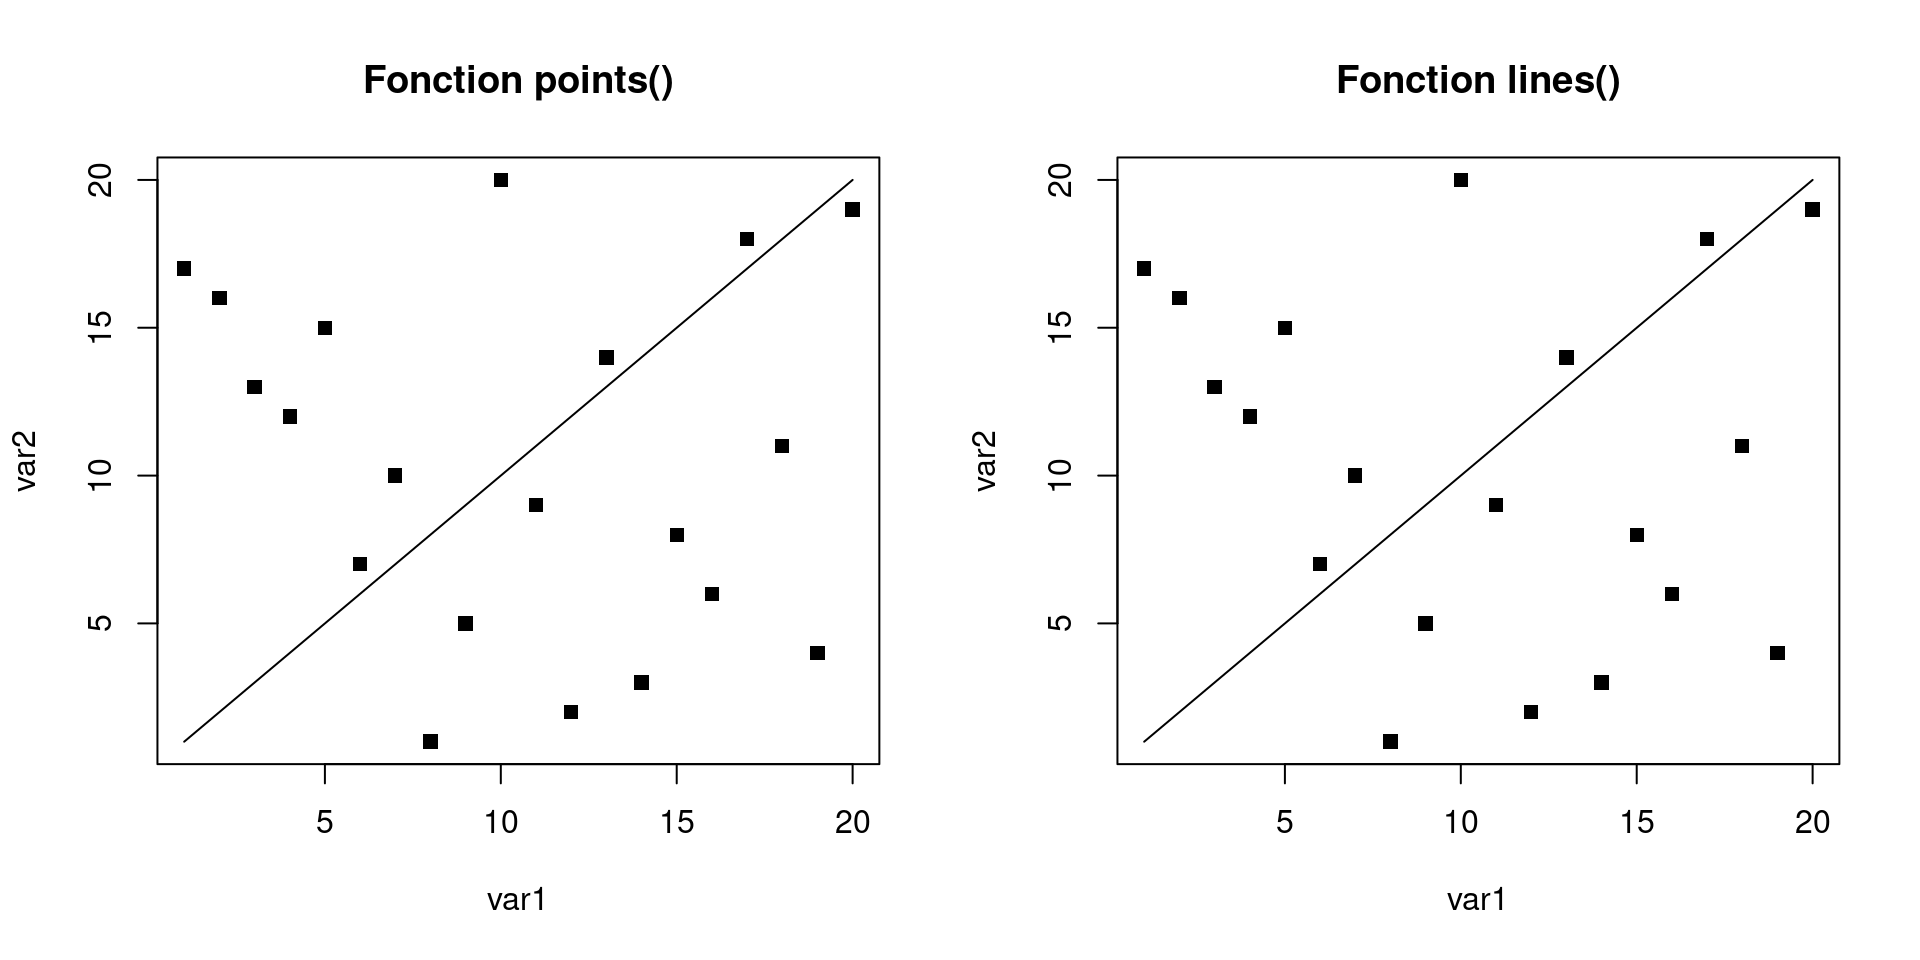
\includegraphics[width=.8\linewidth]{visualiseR_files/figure-latex/unnamed-chunk-16-1} \end{center}

La fonction \texttt{segments()} s'utilise à peu de choses prêt de la même manière.

\begin{Shaded}
\begin{Highlighting}[]
\KeywordTok{par}\NormalTok{(}\DataTypeTok{mfrow =} \KeywordTok{c}\NormalTok{(}\DecValTok{1}\NormalTok{, }\DecValTok{2}\NormalTok{))}
\KeywordTok{plot}\NormalTok{(var1, var2, }\DataTypeTok{pch =} \DecValTok{15}\NormalTok{)}
\KeywordTok{segments}\NormalTok{(}\DataTypeTok{x0 =} \DecValTok{1}\NormalTok{, }\DataTypeTok{y0 =} \DecValTok{1}\NormalTok{, }\DataTypeTok{x1 =} \DecValTok{20}\NormalTok{, }\DataTypeTok{y1 =} \DecValTok{20}\NormalTok{)}
\KeywordTok{plot}\NormalTok{(var1, var2, }\DataTypeTok{pch =} \DecValTok{15}\NormalTok{)}
\KeywordTok{segments}\NormalTok{(var1[}\DecValTok{1}\NormalTok{], var2[}\DecValTok{1}\NormalTok{], var1[}\DecValTok{2}\NormalTok{], var2[}\DecValTok{2}\NormalTok{])}
\KeywordTok{segments}\NormalTok{(var1[}\DecValTok{1}\NormalTok{], var2[}\DecValTok{1}\NormalTok{], var1[}\DecValTok{20}\NormalTok{], var2[}\DecValTok{20}\NormalTok{])}
\KeywordTok{segments}\NormalTok{(var1[}\DecValTok{20}\NormalTok{], var2[}\DecValTok{20}\NormalTok{], var1[}\DecValTok{2}\NormalTok{], var2[}\DecValTok{2}\NormalTok{])}
\end{Highlighting}
\end{Shaded}

\begin{center}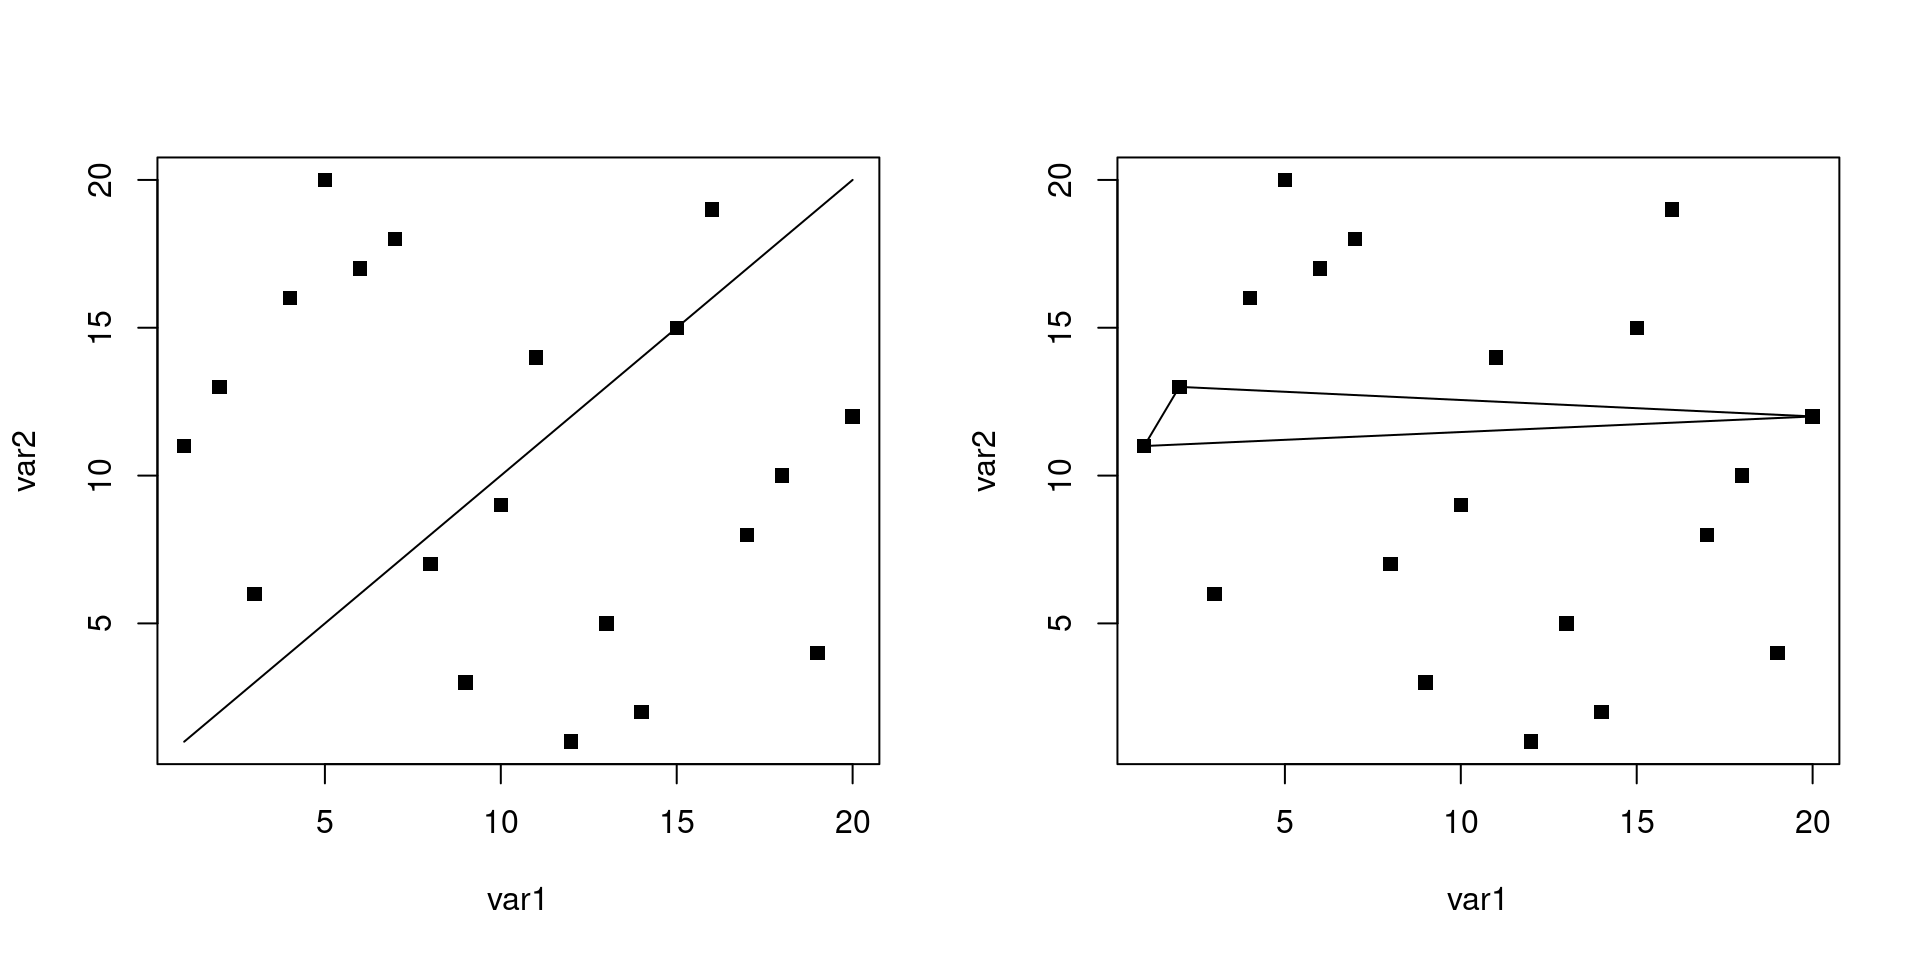
\includegraphics[width=.7\linewidth]{visualiseR_files/figure-latex/unnamed-chunk-17-1} \end{center}

Parlons maintenant de la fonction \texttt{abline()}. Celle-ci offre plusieurs possibilités : elle permet entre autres de tracer des lignes horizontales et verticales ainsi que des droites de régression. Mais, contrairement aux trois fonctions précédentes, qui étaient bornées aux coordonnées fournies, les droites tracées avec cette fonction s'étendront d'un bord à l'autre de la région graphique.

\begin{Shaded}
\begin{Highlighting}[]
\KeywordTok{plot}\NormalTok{(var1, var2, }\DataTypeTok{pch =} \DecValTok{15}\NormalTok{)}
\KeywordTok{abline}\NormalTok{(}\DataTypeTok{h =} \DecValTok{10}\NormalTok{, }\DataTypeTok{v =} \DecValTok{10}\NormalTok{, }\DataTypeTok{col =} \StringTok{"blue"}\NormalTok{)}
\KeywordTok{abline}\NormalTok{(}\DataTypeTok{a =} \DecValTok{20}\NormalTok{, }\DataTypeTok{b =} \DecValTok{-1}\NormalTok{, }\DataTypeTok{col =} \StringTok{"green"}\NormalTok{, }\DataTypeTok{lwd =} \DecValTok{2}\NormalTok{)}
\KeywordTok{abline}\NormalTok{(}\DataTypeTok{reg =} \KeywordTok{lm}\NormalTok{(var2 }\OperatorTok{~}\StringTok{ }\NormalTok{var1), }\DataTypeTok{col =} \StringTok{"red"}\NormalTok{, }\DataTypeTok{lwd =} \DecValTok{2}\NormalTok{)}
\end{Highlighting}
\end{Shaded}

\begin{center}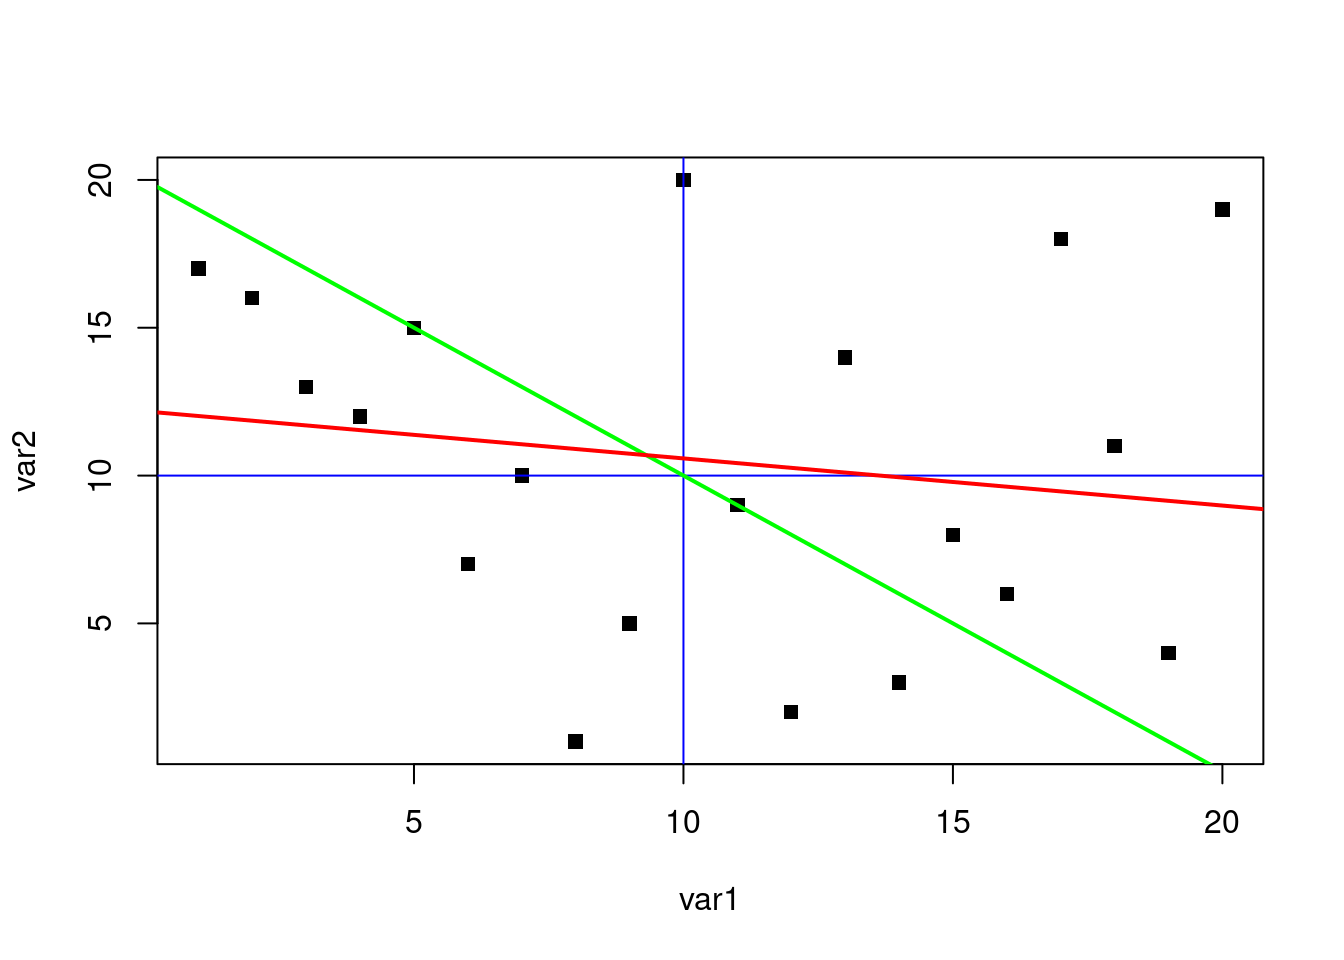
\includegraphics[width=.35\linewidth]{visualiseR_files/figure-latex/unnamed-chunk-18-1} \end{center}

Finalement, mentionnons que la fonction \texttt{locator()} pourra être utilisée pour tracer des lignes de manière interactive.

\begin{Shaded}
\begin{Highlighting}[]
\KeywordTok{locator}\NormalTok{(}\DataTypeTok{n =} \DecValTok{2}\NormalTok{, }\DataTypeTok{type =} \StringTok{"l"}\NormalTok{, }\DataTypeTok{col =} \StringTok{"blue"}\NormalTok{, }\DataTypeTok{lty =} \DecValTok{3}\NormalTok{)}
\KeywordTok{lines}\NormalTok{(}\KeywordTok{locator}\NormalTok{(}\DecValTok{4}\NormalTok{), }\DataTypeTok{col =} \StringTok{"red"}\NormalTok{)}
\end{Highlighting}
\end{Shaded}

\hypertarget{ajout-de-polygones}{%
\subsection{Ajout de polygones}\label{ajout-de-polygones}}

Insérer une forme polygonale sur un graphe se fera à l'aide de la fonction \texttt{polygon()}.

\begin{Shaded}
\begin{Highlighting}[]
\KeywordTok{plot}\NormalTok{(var1, var2, }\DataTypeTok{pch =} \DecValTok{15}\NormalTok{)}
\KeywordTok{polygon}\NormalTok{(}\DataTypeTok{x =} \KeywordTok{c}\NormalTok{(}\DecValTok{10}\NormalTok{, }\DecValTok{5}\NormalTok{, }\DecValTok{5}\NormalTok{, }\DecValTok{10}\NormalTok{, }\DecValTok{15}\NormalTok{, }\DecValTok{15}\NormalTok{), }\DataTypeTok{y =} \KeywordTok{c}\NormalTok{(}\DecValTok{5}\NormalTok{, }\DecValTok{10}\NormalTok{, }\DecValTok{15}\NormalTok{, }\DecValTok{20}\NormalTok{, }\DecValTok{15}\NormalTok{, }\DecValTok{10}\NormalTok{))}
\KeywordTok{polygon}\NormalTok{(}\DataTypeTok{x =} \KeywordTok{c}\NormalTok{(}\DecValTok{10}\NormalTok{, }\DecValTok{5}\NormalTok{, }\DecValTok{15}\NormalTok{), }\DataTypeTok{y =} \KeywordTok{c}\NormalTok{(}\DecValTok{5}\NormalTok{, }\DecValTok{15}\NormalTok{, }\DecValTok{15}\NormalTok{), }\DataTypeTok{density =} \DecValTok{20}\NormalTok{, }\DataTypeTok{angle =} \DecValTok{45}\NormalTok{)}
\KeywordTok{polygon}\NormalTok{(}\DataTypeTok{x =} \KeywordTok{c}\NormalTok{(}\DecValTok{5}\NormalTok{, }\DecValTok{10}\NormalTok{, }\DecValTok{15}\NormalTok{), }\DataTypeTok{y =} \KeywordTok{c}\NormalTok{(}\DecValTok{10}\NormalTok{, }\DecValTok{20}\NormalTok{, }\DecValTok{10}\NormalTok{), }\DataTypeTok{density =} \DecValTok{20}\NormalTok{, }\DataTypeTok{angle =} \DecValTok{135}\NormalTok{)}
\end{Highlighting}
\end{Shaded}

\begin{center}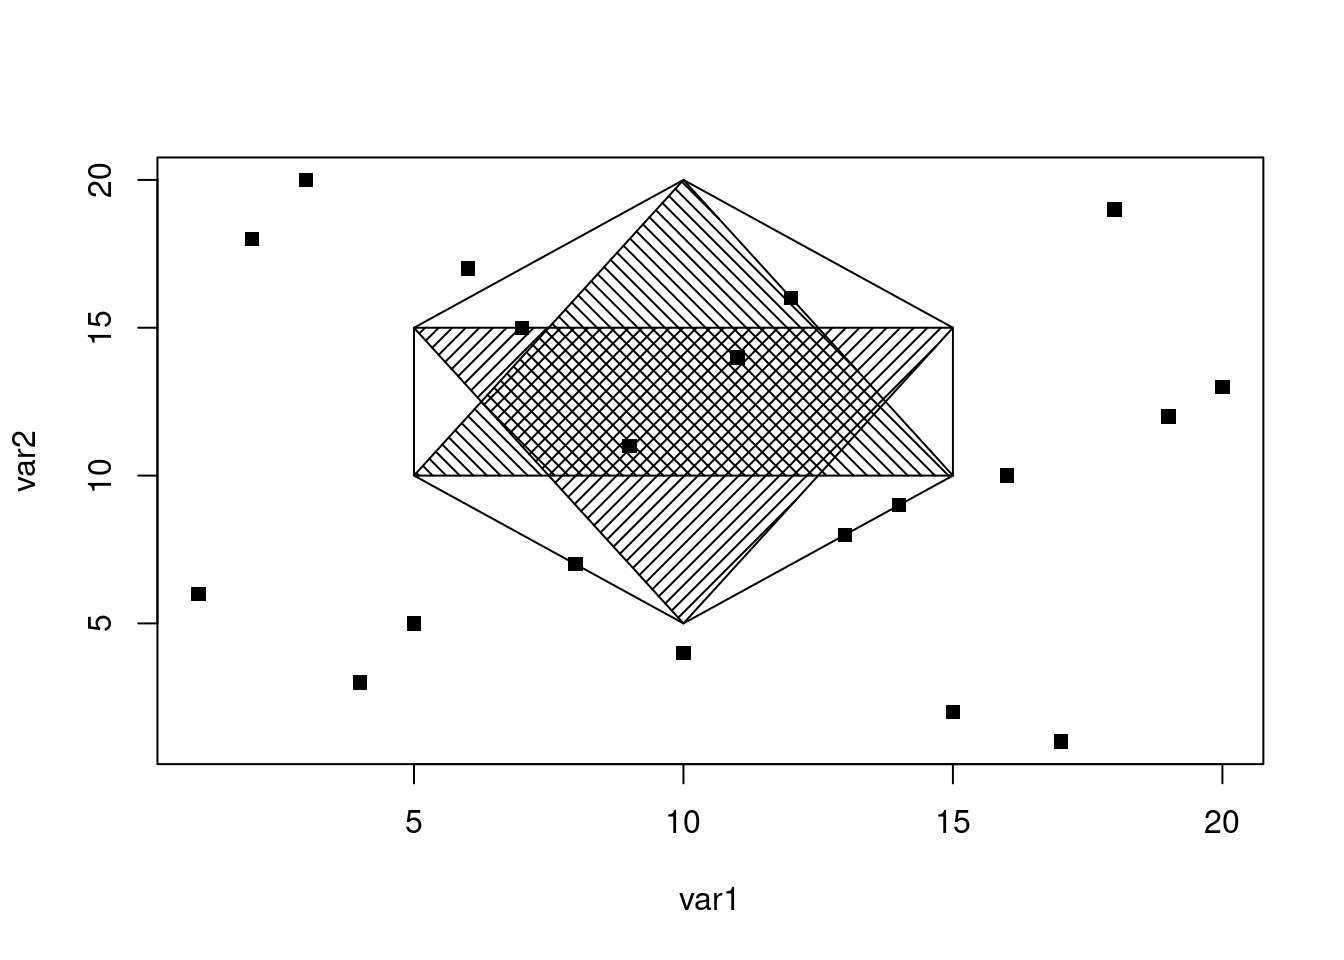
\includegraphics[width=.5\linewidth]{visualiseR_files/figure-latex/unnamed-chunk-20-1} \end{center}

Nous retrouvons ici des arguments vu précédemment dans d'autres fonctions. Voyons maintenant un exemple en couleurs. Nous allons générer trois variables, dont deux correspondant à deux distributions normales.

\begin{Shaded}
\begin{Highlighting}[]
\NormalTok{seqX <-}\StringTok{ }\KeywordTok{seq}\NormalTok{(}\OperatorTok{-}\DecValTok{20}\NormalTok{, }\DecValTok{20}\NormalTok{, }\FloatTok{0.01}\NormalTok{)}
\NormalTok{GaussA <-}\StringTok{ }\KeywordTok{dnorm}\NormalTok{(seqX, }\DataTypeTok{mean =} \DecValTok{-2}\NormalTok{, }\DataTypeTok{sd =} \DecValTok{4}\NormalTok{)}
\NormalTok{GaussB <-}\StringTok{ }\KeywordTok{dnorm}\NormalTok{(seqX, }\DataTypeTok{mean =} \DecValTok{4}\NormalTok{, }\DataTypeTok{sd =} \DecValTok{4}\NormalTok{)}
\end{Highlighting}
\end{Shaded}

Traçons ces distributions avec la fonction \texttt{polygon()}.

\begin{Shaded}
\begin{Highlighting}[]
\KeywordTok{plot}\NormalTok{(}\KeywordTok{range}\NormalTok{(seqX), }\KeywordTok{range}\NormalTok{(GaussA), }\DataTypeTok{type =} \StringTok{"n"}\NormalTok{)}
\KeywordTok{polygon}\NormalTok{(}\DataTypeTok{x =}\NormalTok{ seqX, }\DataTypeTok{y =}\NormalTok{ GaussA, }\DataTypeTok{border =} \DecValTok{0}\NormalTok{, }\DataTypeTok{col =} \StringTok{"#FF000088"}\NormalTok{)}
\KeywordTok{polygon}\NormalTok{(}\DataTypeTok{x =}\NormalTok{ seqX, }\DataTypeTok{y =}\NormalTok{ GaussB, }\DataTypeTok{border =} \DecValTok{0}\NormalTok{, }\DataTypeTok{col =} \StringTok{"#0000FF88"}\NormalTok{)}
\end{Highlighting}
\end{Shaded}

\begin{center}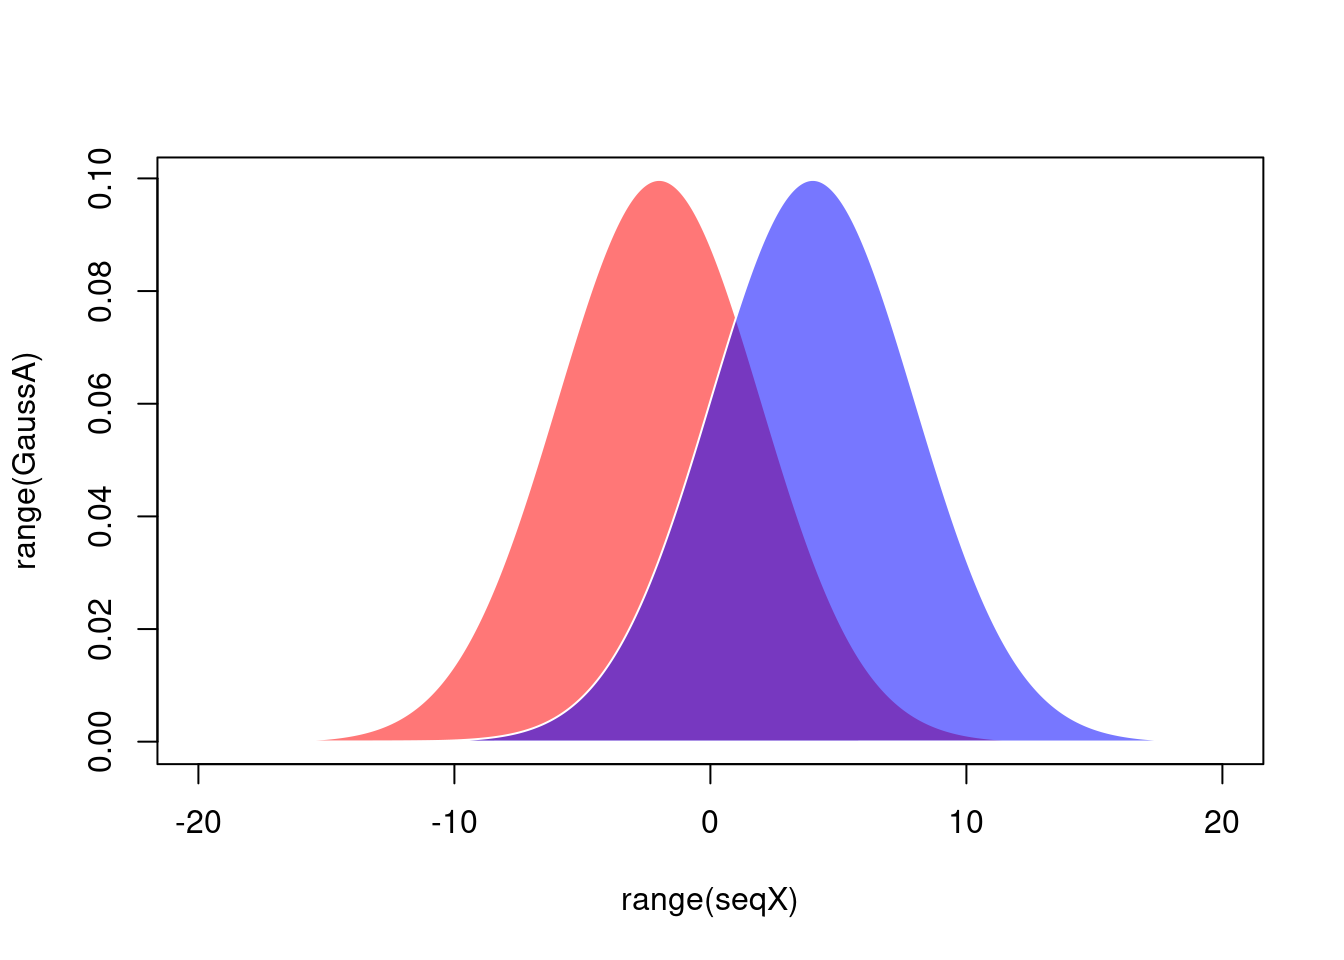
\includegraphics[width=.45\linewidth]{visualiseR_files/figure-latex/unnamed-chunk-22-1} \end{center}

Ici, une remarque s'impose : nous venons d'attribuer deux couleurs dans un format un peu spécial : il s'agit du format hexadécimal. Celui-ci comprend, dans sa forme minimale, six caractères précédés du symbole \emph{dièse} : les deux premiers symboles reflètent la quantité de rouge, les deux suivants celle de vert, et les deux derniers la quantité de bleu. À ceci, on peut rajouter (comme nous l'avons fait) deux autres caractères représentant le degré de transparence. Nous reviendrons sur ce point dans le chapitre suivant.
Intéressons-nous maintenant à la fonction \texttt{rect()} qui permet de tracer un rectangle.

\begin{Shaded}
\begin{Highlighting}[]
\KeywordTok{plot}\NormalTok{(var1, var2, }\DataTypeTok{pch =} \DecValTok{15}\NormalTok{)}
\KeywordTok{rect}\NormalTok{(}\DataTypeTok{xleft =} \DecValTok{5}\NormalTok{, }\DataTypeTok{ybottom =} \DecValTok{5}\NormalTok{, }\DataTypeTok{xright =} \DecValTok{15}\NormalTok{, }\DataTypeTok{ytop =} \DecValTok{15}\NormalTok{, }\DataTypeTok{col =} \StringTok{"gray"}\NormalTok{)}
\end{Highlighting}
\end{Shaded}

\begin{center}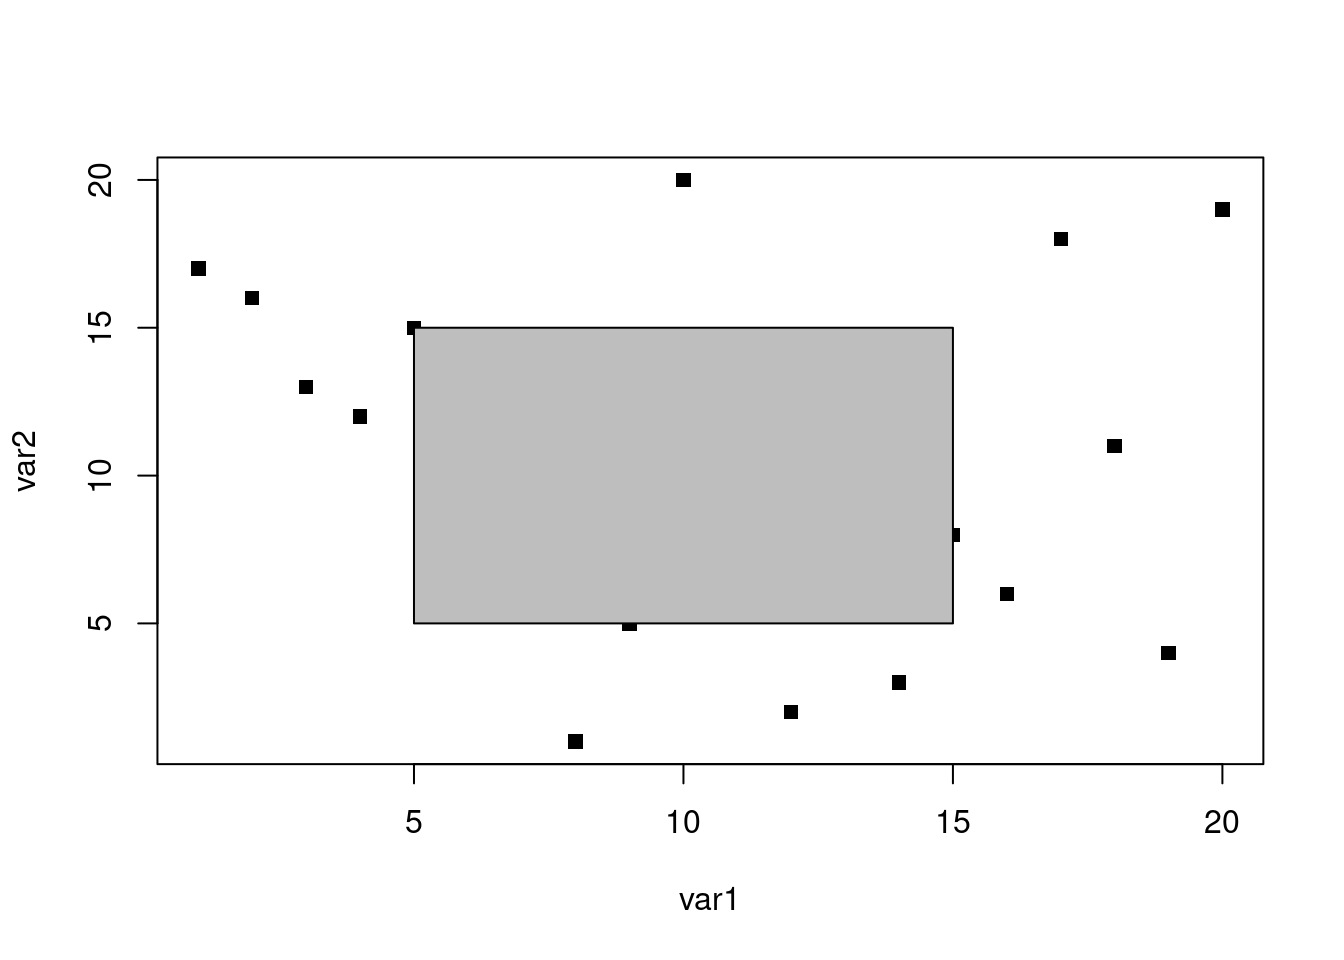
\includegraphics[width=.45\linewidth]{visualiseR_files/figure-latex/unnamed-chunk-23-1} \end{center}

Remarque : la fonction \texttt{locator()} peut également être utilisée avec \texttt{polygon()}, mais pas avec la fonction \texttt{rect()}.
Mettons à profit ce que nous venons d'apprendre avec les fonctions \texttt{rect()} et \texttt{abline()} pour personnaliser la zone de plot.

\begin{Shaded}
\begin{Highlighting}[]
\KeywordTok{plot}\NormalTok{(}\DecValTok{0}\NormalTok{, }\DataTypeTok{type =} \StringTok{"n"}\NormalTok{, }\DataTypeTok{xlim =} \KeywordTok{c}\NormalTok{(}\DecValTok{0}\NormalTok{, }\DecValTok{20}\NormalTok{), }\DataTypeTok{ylim =} \KeywordTok{c}\NormalTok{(}\DecValTok{0}\NormalTok{, }\DecValTok{20}\NormalTok{), }\DataTypeTok{ann =} \OtherTok{FALSE}\NormalTok{, }\DataTypeTok{las =} \DecValTok{1}\NormalTok{, }\DataTypeTok{bty =} \StringTok{"n"}\NormalTok{)}
\KeywordTok{par}\NormalTok{()}\OperatorTok{$}\NormalTok{usr}
\CommentTok{#> [1] -0.8 20.8 -0.8 20.8}
\KeywordTok{rect}\NormalTok{(}\DataTypeTok{xleft =} \KeywordTok{par}\NormalTok{()}\OperatorTok{$}\NormalTok{usr[}\DecValTok{1}\NormalTok{], }\DataTypeTok{ybottom =} \KeywordTok{par}\NormalTok{()}\OperatorTok{$}\NormalTok{usr[}\DecValTok{3}\NormalTok{], }\DataTypeTok{ytop =} \KeywordTok{par}\NormalTok{()}\OperatorTok{$}\NormalTok{usr[}\DecValTok{4}\NormalTok{], }\DataTypeTok{xright =} \KeywordTok{par}\NormalTok{()}\OperatorTok{$}\NormalTok{usr[}\DecValTok{2}\NormalTok{], }\DataTypeTok{col =} \StringTok{"lightgray"}\NormalTok{, }\DataTypeTok{border =} \DecValTok{0}\NormalTok{)}
\KeywordTok{abline}\NormalTok{(}\DataTypeTok{h =} \KeywordTok{seq}\NormalTok{(}\DecValTok{0}\NormalTok{, }\DecValTok{20}\NormalTok{, }\DataTypeTok{by =} \DecValTok{5}\NormalTok{), }\DataTypeTok{col =} \StringTok{"white"}\NormalTok{)}
\KeywordTok{abline}\NormalTok{(}\DataTypeTok{v =} \KeywordTok{seq}\NormalTok{(}\DecValTok{0}\NormalTok{, }\DecValTok{20}\NormalTok{, }\DataTypeTok{by =} \DecValTok{5}\NormalTok{), }\DataTypeTok{col =} \StringTok{"white"}\NormalTok{)}
\KeywordTok{abline}\NormalTok{(}\DataTypeTok{h =} \KeywordTok{seq}\NormalTok{(}\FloatTok{2.5}\NormalTok{, }\FloatTok{17.5}\NormalTok{, }\DataTypeTok{by =} \DecValTok{5}\NormalTok{), }\DataTypeTok{col =} \StringTok{"white"}\NormalTok{, }\DataTypeTok{lty =} \DecValTok{3}\NormalTok{)}
\KeywordTok{abline}\NormalTok{(}\DataTypeTok{v =} \KeywordTok{seq}\NormalTok{(}\FloatTok{2.5}\NormalTok{, }\FloatTok{17.5}\NormalTok{, }\DataTypeTok{by =} \DecValTok{5}\NormalTok{), }\DataTypeTok{col =} \StringTok{"white"}\NormalTok{, }\DataTypeTok{lty =} \DecValTok{3}\NormalTok{)}
\KeywordTok{rect}\NormalTok{(}\DataTypeTok{xleft =} \KeywordTok{par}\NormalTok{()}\OperatorTok{$}\NormalTok{usr[}\DecValTok{1}\NormalTok{], }\DataTypeTok{ybottom =} \KeywordTok{par}\NormalTok{()}\OperatorTok{$}\NormalTok{usr[}\DecValTok{3}\NormalTok{], }\DataTypeTok{ytop =} \KeywordTok{par}\NormalTok{()}\OperatorTok{$}\NormalTok{usr[}\DecValTok{4}\NormalTok{], }\DataTypeTok{xright =} \KeywordTok{par}\NormalTok{()}\OperatorTok{$}\NormalTok{usr[}\DecValTok{2}\NormalTok{], }\DataTypeTok{col =} \DecValTok{0}\NormalTok{, }\DataTypeTok{border =} \StringTok{"white"}\NormalTok{)}
\end{Highlighting}
\end{Shaded}

\begin{center}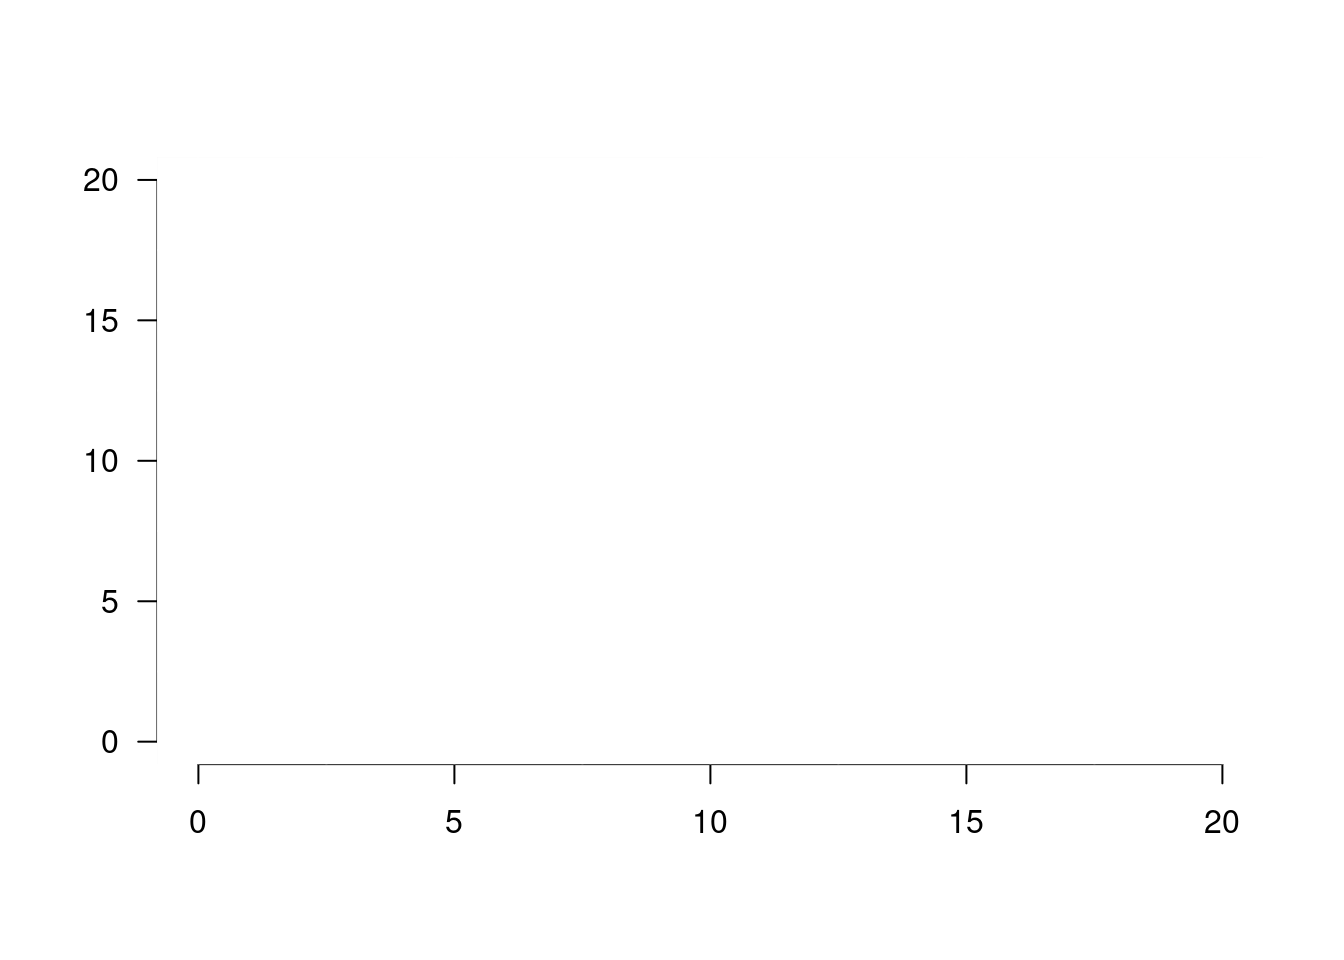
\includegraphics[width=.75\linewidth]{visualiseR_files/figure-latex/unnamed-chunk-24-1} \end{center}

Ici, nous avons utilisé de nouveaux arguments. L'argument \texttt{lty} contrôle le type de ligne (\textbf{1} étant un trait plein, et \textbf{3} un trait en pointillés). L'argument \texttt{border\ =\ 0} indique que la couleur du contour du rectangle sera transparente. Enfin, l'argument \texttt{las\ =\ 1} spécifie que les valeurs portées sur les axes seront écrites horizontalement.
Quelques précisions maintenant sur la commande \texttt{par()\textbackslash{}\$usr}. Nous avons défini nous-même l'étendue des axes x et y (0, 20). Cependant, par défaut, R laisse un peu de marge avant et après chaque axe (4\% pour être précis). Ainsi, cette commande nous permet de récupérer les dimensions exactes (après ajout de ces 4\%) de la région du plot. En attribuant la valeur \textbf{``i''} aux paramètres graphiques \texttt{xaxs} et \texttt{yaxs}, nous aurions supprimé cet ajout de 4\%. Pour preuve :

\begin{Shaded}
\begin{Highlighting}[]
\KeywordTok{plot}\NormalTok{(}\DecValTok{0}\NormalTok{, }\DataTypeTok{xlim =} \KeywordTok{c}\NormalTok{(}\DecValTok{0}\NormalTok{, }\DecValTok{20}\NormalTok{), }\DataTypeTok{ylim =} \KeywordTok{c}\NormalTok{(}\DecValTok{0}\NormalTok{, }\DecValTok{20}\NormalTok{), }\DataTypeTok{xaxs =} \StringTok{"i"}\NormalTok{, }\DataTypeTok{yaxs =} \StringTok{"i"}\NormalTok{)}
\KeywordTok{par}\NormalTok{()}\OperatorTok{$}\NormalTok{usr}
\CommentTok{#> [1]  0 20  0 20}
\end{Highlighting}
\end{Shaded}

\hypertarget{ajout-dune-fluxe8che}{%
\subsection{Ajout d'une flèche}\label{ajout-dune-fluxe8che}}

Bien que peu fréquent, nous pouvons aussi tracer des flèches. Ceci se fera avec la fonction \texttt{arrows()}. Nous pouvons spécifier si la flèche sera en début ou en fin de ligne (ou les deux) avec l'argument \texttt{code}. On peut aussi définir la longueur de la flèche et son angle par rapport au trait. Un dessin vaut mille mots, donc allons-y.

\begin{Shaded}
\begin{Highlighting}[]
\KeywordTok{plot}\NormalTok{(}\DecValTok{0}\NormalTok{, }\DataTypeTok{xlim =} \KeywordTok{c}\NormalTok{(}\DecValTok{0}\NormalTok{, }\DecValTok{2}\NormalTok{), }\DataTypeTok{ylim =} \KeywordTok{c}\NormalTok{(}\DecValTok{0}\NormalTok{, }\DecValTok{2}\NormalTok{), }\DataTypeTok{type =} \StringTok{"n"}\NormalTok{, }\DataTypeTok{ann =} \OtherTok{FALSE}\NormalTok{)}
\KeywordTok{arrows}\NormalTok{(}\DataTypeTok{x0 =} \DecValTok{0}\NormalTok{, }\DataTypeTok{y0 =} \DecValTok{1}\NormalTok{, }\DataTypeTok{x1 =} \DecValTok{1}\NormalTok{, }\DataTypeTok{y1 =} \DecValTok{2}\NormalTok{)}
\KeywordTok{arrows}\NormalTok{(}\DecValTok{1}\NormalTok{, }\DecValTok{0}\NormalTok{, }\DecValTok{2}\NormalTok{, }\DecValTok{1}\NormalTok{, }\DataTypeTok{length =} \FloatTok{0.25}\NormalTok{, }\DataTypeTok{angle =} \DecValTok{30}\NormalTok{, }\DataTypeTok{code =} \DecValTok{1}\NormalTok{)}
\KeywordTok{arrows}\NormalTok{(}\DecValTok{1}\NormalTok{, }\FloatTok{0.5}\NormalTok{, }\DecValTok{1}\NormalTok{, }\FloatTok{1.5}\NormalTok{, }\DataTypeTok{length =} \FloatTok{0.10}\NormalTok{, }\DataTypeTok{angle =} \DecValTok{45}\NormalTok{, }\DataTypeTok{code =} \DecValTok{3}\NormalTok{)}
\end{Highlighting}
\end{Shaded}

\begin{center}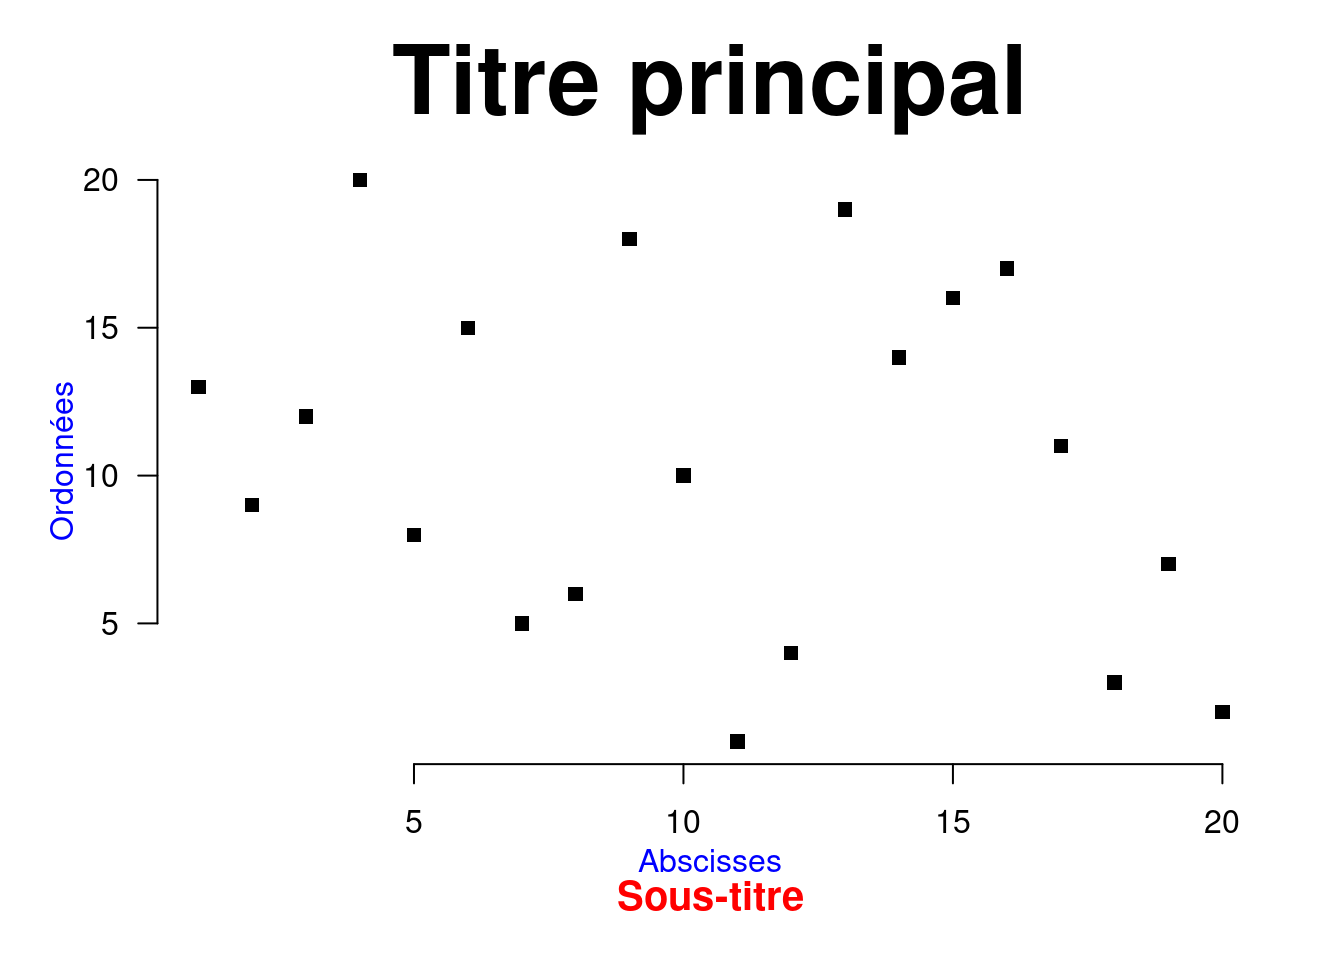
\includegraphics[width=.5\linewidth]{visualiseR_files/figure-latex/unnamed-chunk-26-1} \end{center}

Nous n'en dirons pas plus sur les flèches.

\hypertarget{ajout-dun-titre}{%
\subsection{Ajout d'un titre}\label{ajout-dun-titre}}

Précédemment, nous avons vu qu'il était possible de définir un titre directement dans les \emph{High-level plotting functions}. Mais, il existe aussi la fonction \texttt{title()} en alternative. Voici les principaux arguments de cette fonction (qui sont aussi valables pour les fonctions \texttt{plot()} and co.).
\{ll\}

\textbf{Argument} \& \textbf{Signification}:

\begin{itemize}
\tightlist
\item
  \texttt{main} \& Titre principal
\item
  \texttt{sub} \& Sous-titre
\item
  \texttt{xlab} \& Nom de l'axe des x
\item
  \texttt{ylab} \& Nom de l'axe des y
\item
  \texttt{cex.main} \& Taille du titre
\item
  \texttt{cex.sub} \& Taille du sous-titre
\end{itemize}

Utilisons ces arguments.

\begin{Shaded}
\begin{Highlighting}[]
\KeywordTok{par}\NormalTok{(}\DataTypeTok{mgp =} \KeywordTok{c}\NormalTok{(}\DecValTok{2}\NormalTok{, }\DecValTok{1}\NormalTok{, }\DecValTok{0}\NormalTok{))}
\KeywordTok{plot}\NormalTok{(var1, var2, }\DataTypeTok{pch =} \DecValTok{15}\NormalTok{, }\DataTypeTok{ann =} \OtherTok{FALSE}\NormalTok{, }\DataTypeTok{las =} \DecValTok{1}\NormalTok{, }\DataTypeTok{bty =} \StringTok{"n"}\NormalTok{)}
\KeywordTok{title}\NormalTok{(}\DataTypeTok{main =} \StringTok{"Titre principal"}\NormalTok{, }\DataTypeTok{cex.main =} \DecValTok{3}\NormalTok{)}
\KeywordTok{title}\NormalTok{(}\DataTypeTok{xlab =} \StringTok{"Abscisses"}\NormalTok{, }\DataTypeTok{ylab =} \StringTok{"Ordonnées"}\NormalTok{, }\DataTypeTok{col.lab =} \StringTok{"blue"}\NormalTok{)}
\KeywordTok{title}\NormalTok{(}\DataTypeTok{sub =} \StringTok{"Sous-titre"}\NormalTok{, }\DataTypeTok{font.sub =} \DecValTok{2}\NormalTok{, }\DataTypeTok{col.sub =} \StringTok{"red"}\NormalTok{, }\DataTypeTok{cex.sub =} \FloatTok{1.25}\NormalTok{)}
\end{Highlighting}
\end{Shaded}

\begin{center}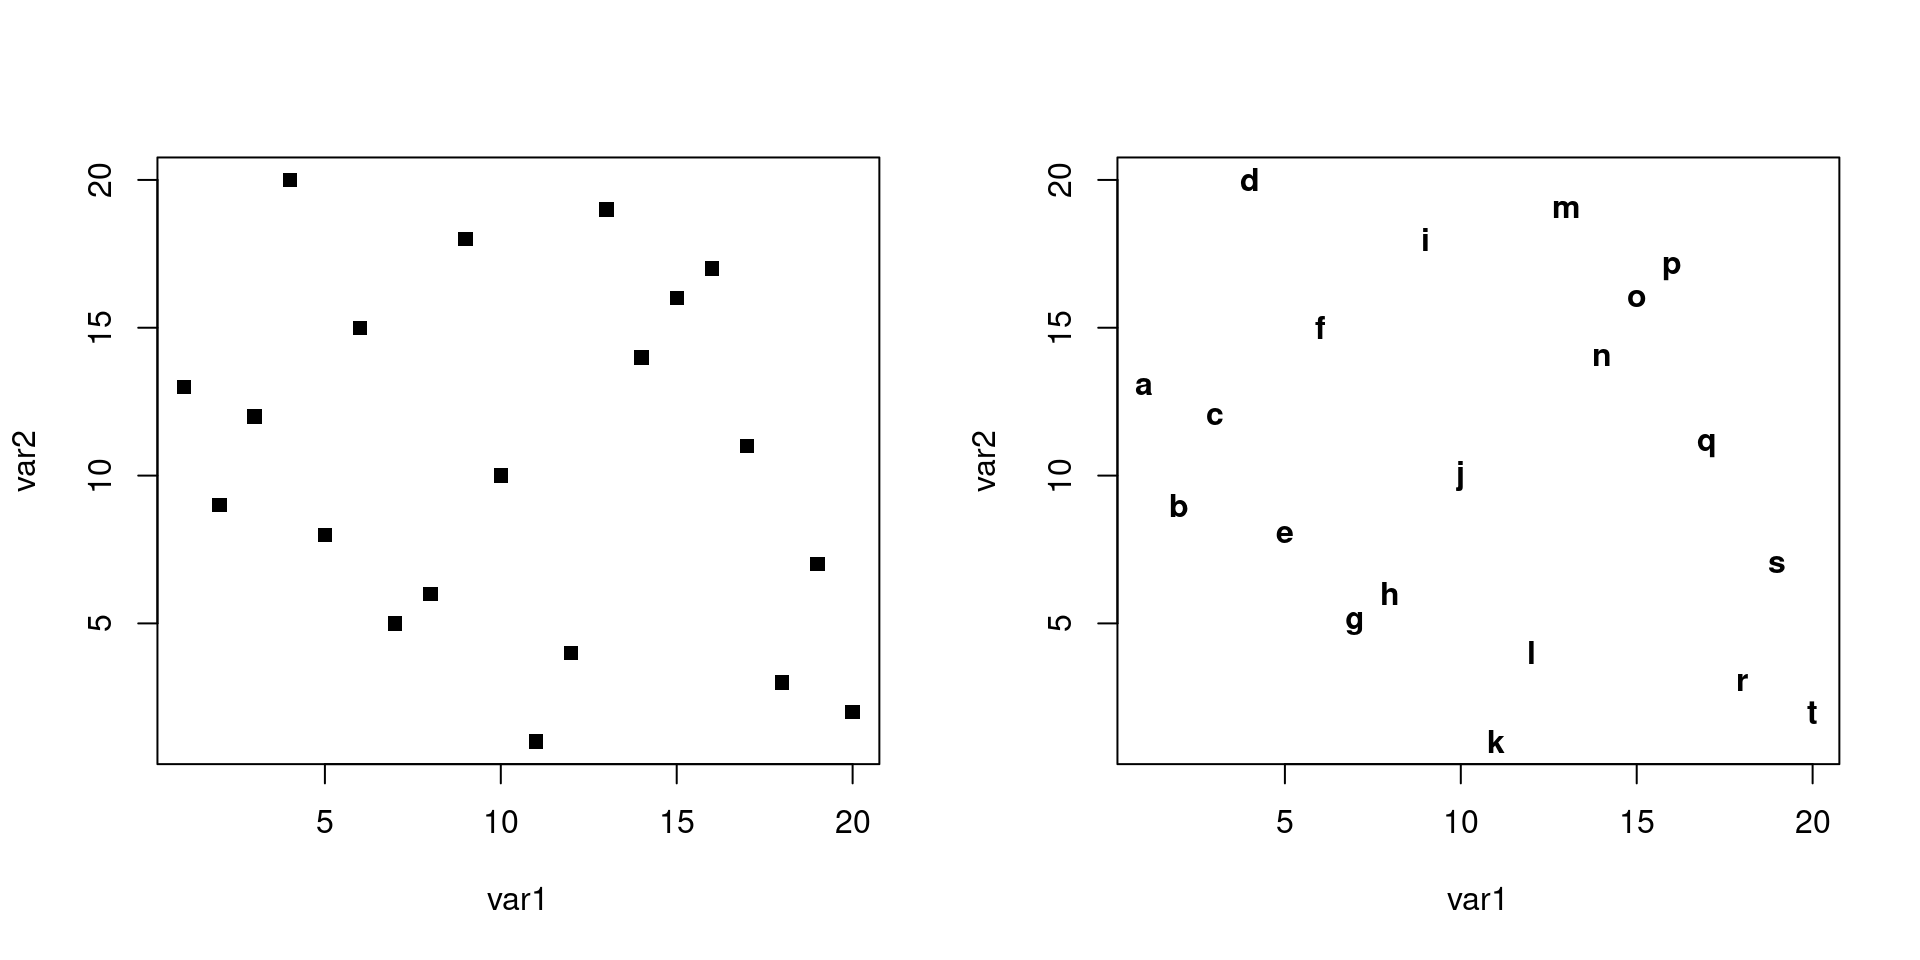
\includegraphics[width=.6\linewidth]{visualiseR_files/figure-latex/unnamed-chunk-27-1} \end{center}

Nous verrons dans la section suivante qu'il est aussi possible d'ajouter des annotations dans les marges de la figure, et nous aurions pu utiliser à la place, la fonction \texttt{mtext()}.

\hypertarget{ajout-de-texte}{%
\subsection{Ajout de texte}\label{ajout-de-texte}}

Intéressons-nous maintenant aux annotations textuelles. Nous distinguerons les expressions textuelles insérées dans la zone de plot de celles destinées à apparaître en dehors de cette zone, c.-à-d. dans les marges de la figure. En effet, les fonctions correspondantes ne sont pas les mêmes et ne s'écrivent pas de la même manière.

La fonction \texttt{text()} permet d'insérer du texte dans la région du plot. Il faudra lui fournir les coordonnées en x et en y, ainsi que l'expression textuelle à ajouter. Regardons cela au travers d'un exemple.

\begin{Shaded}
\begin{Highlighting}[]
\NormalTok{(nom <-}\StringTok{ }\NormalTok{letters[}\KeywordTok{seq_along}\NormalTok{(var1)])}
\CommentTok{#>  [1] "a" "b" "c" "d" "e" "f" "g" "h" "i" "j" "k" "l" "m" "n" "o" "p" "q" "r" "s"}
\CommentTok{#> [20] "t"}
\KeywordTok{par}\NormalTok{(}\DataTypeTok{mfrow =} \KeywordTok{c}\NormalTok{(}\DecValTok{1}\NormalTok{, }\DecValTok{2}\NormalTok{))}
\KeywordTok{plot}\NormalTok{(var1, var2, }\DataTypeTok{pch =} \DecValTok{15}\NormalTok{)}
\KeywordTok{plot}\NormalTok{(var1, var2, }\DataTypeTok{type =} \StringTok{"n"}\NormalTok{)}
\KeywordTok{text}\NormalTok{(}\DataTypeTok{x =}\NormalTok{ var1, }\DataTypeTok{y =}\NormalTok{ var2, }\DataTypeTok{labels =}\NormalTok{ nom, }\DataTypeTok{font =} \DecValTok{2}\NormalTok{)}
\end{Highlighting}
\end{Shaded}

\begin{center}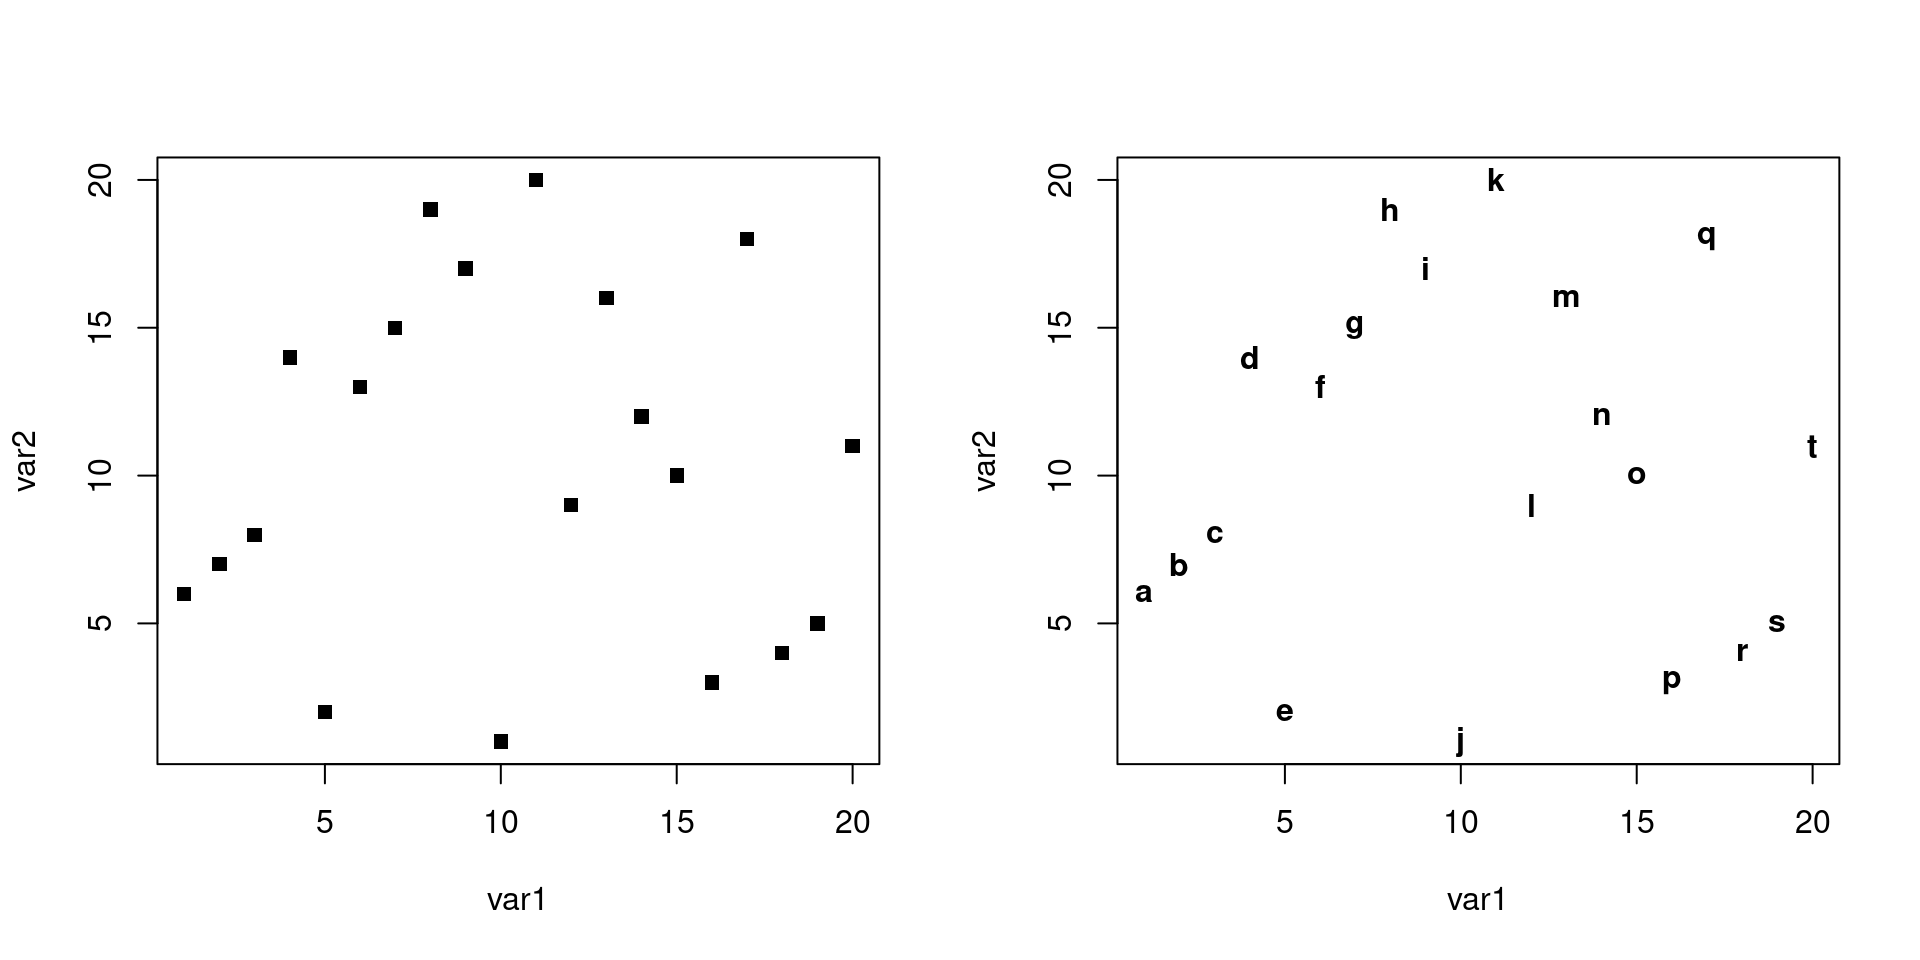
\includegraphics[width=.7\linewidth]{visualiseR_files/figure-latex/unnamed-chunk-28-1} \end{center}

L'argument \texttt{font} contrôle la graisse du texte, c.-à-d. que le texte pourra être écrit normalement (\textbf{1}), en gras (\textbf{2}), en italique (\textbf{3}), etc. Ici, le texte se place exactement aux coordonnées fournies. Mais, on imagine facilement que si on superpose à la fois les points et les étiquettes, le graphique sera illisible. Heureusement, cette fonction présente l'argument \texttt{pos} qui contrôle le positionnement du texte par rapport aux coordonnées. Le tableau suivant fournit les valeurs possibles pour cet argument.

\textbf{Valeur de \texttt{pos}} \& \textbf{Signification}\textbackslash{}
- \texttt{0} \& Aux coordonnées
- \texttt{1} \& En-dessous des coordonnées
- \texttt{2} \& À gauche des coordonnées
- \texttt{3} \& Au-dessus des coordonnées
- \texttt{4} \& À droite des coordonnées

\begin{Shaded}
\begin{Highlighting}[]
\KeywordTok{plot}\NormalTok{(var1, var2, }\DataTypeTok{pch =} \DecValTok{15}\NormalTok{, }\DataTypeTok{ann =} \OtherTok{FALSE}\NormalTok{, }\DataTypeTok{las =} \DecValTok{1}\NormalTok{)}
\KeywordTok{text}\NormalTok{(}\DataTypeTok{x =}\NormalTok{ var1, }\DataTypeTok{y =}\NormalTok{ var2, }\DataTypeTok{labels =}\NormalTok{ nom, }\DataTypeTok{pos =} \DecValTok{2}\NormalTok{)}
\end{Highlighting}
\end{Shaded}

\begin{center}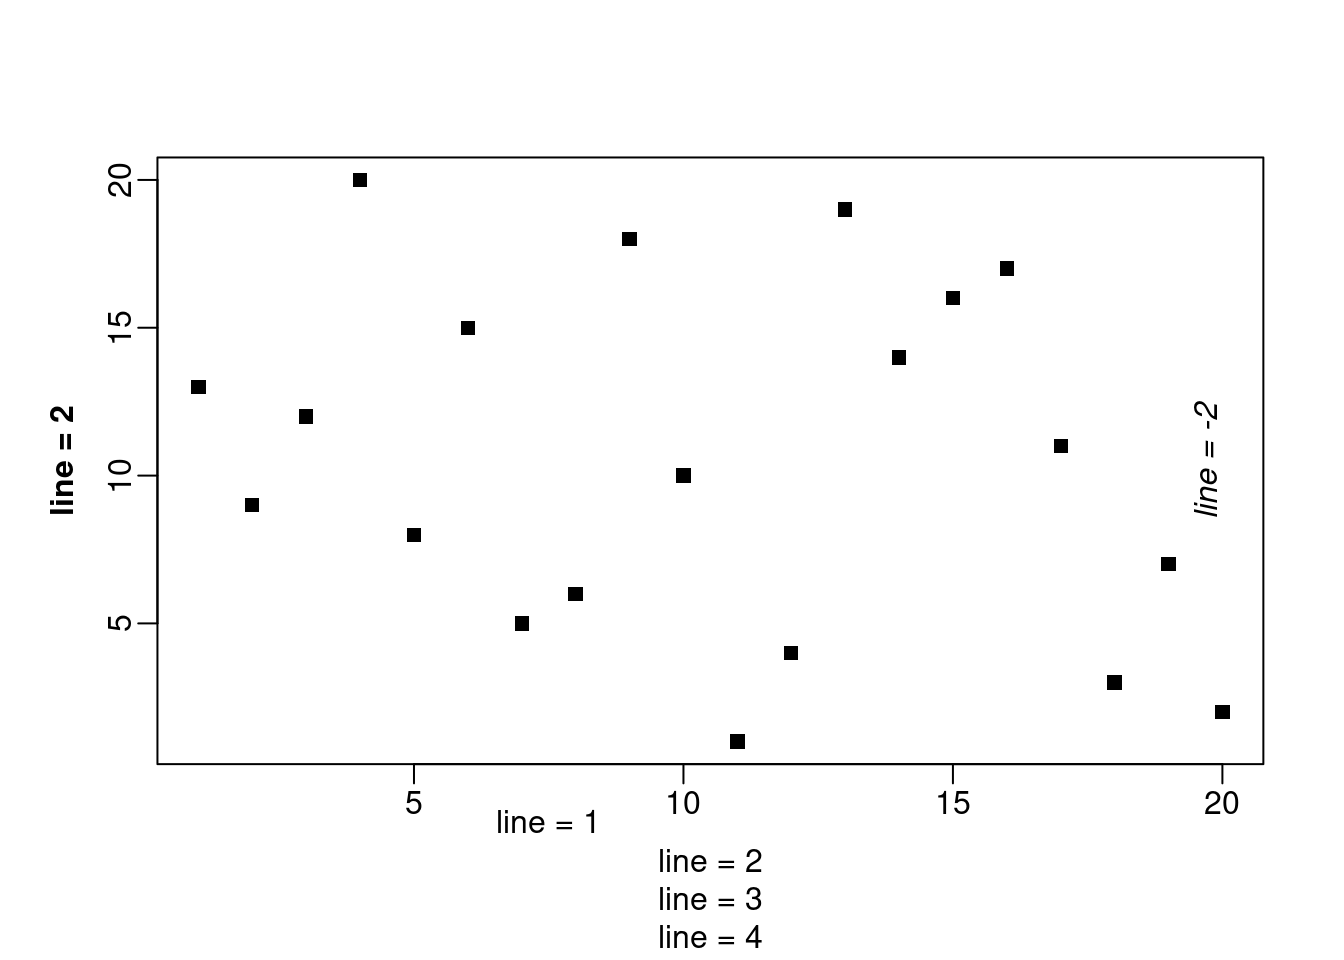
\includegraphics[width=.6\linewidth]{visualiseR_files/figure-latex/unnamed-chunk-29-1} \end{center}

Remarque : la fonction \texttt{locator()} pourra s'appliquer ici.
Pour rajouter du texte dans les marges, nous utiliserons la fonction \texttt{mtext()}. Cependant, cette fonction s'écrit différemment : l'argument \texttt{side} indique dans quelle marge doit être affiché le texte (\textbf{1} en bas, \textbf{2} à gauche, \textbf{3} en haut, \textbf{4} à droite). L'argument \texttt{line} permet quant à lui de positionner le texte par rapport aux limites de la région du plot. Enfin, l'argument \texttt{at} permet d'indiquer la coordonnée de placement sur l'axe en question.
Vu qu'on ne fournit pas de coordonnées dans cette fonction, la fonction \texttt{locator()} ne fonctionnera pas.

Regardons cela avec un exemple simple.

\begin{Shaded}
\begin{Highlighting}[]
\KeywordTok{par}\NormalTok{(}\DataTypeTok{mgp =} \KeywordTok{c}\NormalTok{(}\DecValTok{2}\NormalTok{, }\FloatTok{.5}\NormalTok{, }\DecValTok{0}\NormalTok{))}
\KeywordTok{plot}\NormalTok{(var1, var2, }\DataTypeTok{pch =} \DecValTok{15}\NormalTok{, }\DataTypeTok{ann =} \OtherTok{FALSE}\NormalTok{)}
\KeywordTok{mtext}\NormalTok{(}\DataTypeTok{side =} \DecValTok{1}\NormalTok{, }\DataTypeTok{line =} \DecValTok{1}\NormalTok{, }\DataTypeTok{text =} \StringTok{"line = 1"}\NormalTok{, }\DataTypeTok{at =} \FloatTok{7.5}\NormalTok{)}
\KeywordTok{mtext}\NormalTok{(}\DataTypeTok{side =} \DecValTok{1}\NormalTok{, }\DataTypeTok{line =} \DecValTok{2}\NormalTok{, }\DataTypeTok{text =} \StringTok{"line = 2"}\NormalTok{)}
\KeywordTok{mtext}\NormalTok{(}\DataTypeTok{side =} \DecValTok{1}\NormalTok{, }\DataTypeTok{line =} \DecValTok{3}\NormalTok{, }\DataTypeTok{text =} \StringTok{"line = 3"}\NormalTok{)}
\KeywordTok{mtext}\NormalTok{(}\DataTypeTok{side =} \DecValTok{1}\NormalTok{, }\DataTypeTok{line =} \DecValTok{4}\NormalTok{, }\DataTypeTok{text =} \StringTok{"line = 4"}\NormalTok{)}
\KeywordTok{mtext}\NormalTok{(}\DataTypeTok{side =} \DecValTok{2}\NormalTok{, }\DataTypeTok{line =} \DecValTok{2}\NormalTok{, }\DataTypeTok{text =} \StringTok{"line = 2"}\NormalTok{, }\DataTypeTok{font =} \DecValTok{2}\NormalTok{)}
\KeywordTok{mtext}\NormalTok{(}\DataTypeTok{side =} \DecValTok{4}\NormalTok{, }\DataTypeTok{line =} \DecValTok{-2}\NormalTok{, }\DataTypeTok{text =} \StringTok{"line = -2"}\NormalTok{, }\DataTypeTok{font =} \DecValTok{3}\NormalTok{)}
\end{Highlighting}
\end{Shaded}

\begin{center}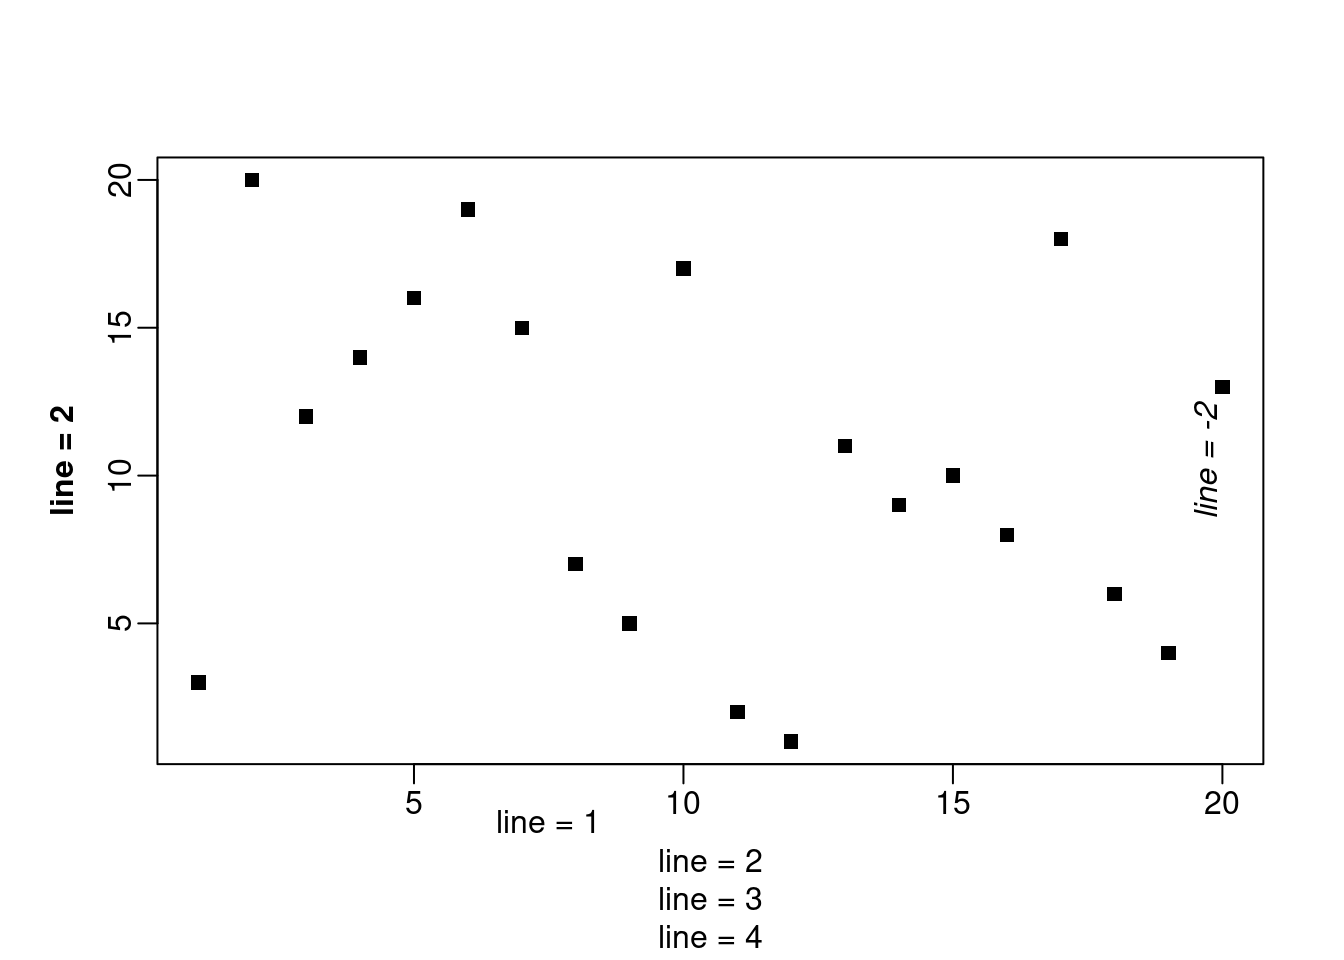
\includegraphics[width=.6\linewidth]{visualiseR_files/figure-latex/unnamed-chunk-30-1} \end{center}

\hypertarget{ajout-dune-luxe9gende}{%
\subsection{Ajout d'une légende}\label{ajout-dune-luxe9gende}}

Que serait un graphe sans légende ? La fonction \texttt{legend()} permet d'insérer une légende assez élaborée dans la région du plot et offre de nombreuses possibilités.

\begin{Shaded}
\begin{Highlighting}[]
\KeywordTok{example}\NormalTok{(legend)}
\end{Highlighting}
\end{Shaded}

Tous les éléments de la légende sont modifiables, à l'exception de la police de caractères, ce qui peut être problématique si les autres éléments textuels du graphe (titre, nom des axes, etc.) n'utilisent pas la police par défaut. Nous verrons comment contourner cette difficulté plus loin.
Le positionnement de la légende peut s'effectuer de deux manières différentes :
- soit en indiquant les coordonnées x et y du coin supérieur gauche;
- soit en spécifiant un mot-clé prédéfini (\texttt{top}, \texttt{bottom}, \texttt{topleft}, \texttt{center}, etc.).
Le tableau ci-après présente les principaux arguments de cette fonction \texttt{legend()}.
\{ll\}

\textbf{Argument} \& \textbf{Signification}

\begin{itemize}
\tightlist
\item
  \texttt{legend} \& Nom des items
\item
  \texttt{bty} \& Type de boîte (défaut \textbf{`o'})
\item
  \texttt{bg} \& Couleur du fond de la boîte
\item
  \texttt{box.lwd} \& Épaisseur de la bordure de la boîte
\item
  \texttt{box.col} \& Couleur de la bordure de la boîte
\item
  \texttt{title} \& Titre de la légende
\item
  \texttt{title.col} \& Couleur du titre
\item
  \texttt{text.col} \& Couleurs du nom des items
\item
  \texttt{text.font} \& Graisse du nom des items
\item
  \texttt{col} \& Couleurs des items (lignes ou symboles)
\item
  \texttt{cex} \& Taille des symboles
\item
  \texttt{pch} \& Symbole des items
\item
  \texttt{pt.cex} \& Taille des symboles
\item
  \texttt{lty} \& Type de ligne (si les items sont des lignes)
\item
  \texttt{lwd} \& Épaisseur des lignes (si les items sont des lignes)
\item
  \texttt{ncol} \& Nombre de colonnes pour représenter les items
\item
  \texttt{horiz} \& Items répartis en lignes ou en colonnes (défaut)
\item
  \texttt{plot} \& \textbf{TRUE} ou \textbf{FALSE}
\end{itemize}

Cette fonction, si attribuée à un objet, retourne des informations intéressantes sur le positionnement et les dimensions de la légende. Regardons plutôt.

\begin{Shaded}
\begin{Highlighting}[]
\KeywordTok{plot}\NormalTok{(var1, var2, }\DataTypeTok{xlim =} \KeywordTok{c}\NormalTok{(}\DecValTok{0}\NormalTok{, }\DecValTok{20}\NormalTok{), }\DataTypeTok{ylim =} \KeywordTok{c}\NormalTok{(}\DecValTok{0}\NormalTok{, }\DecValTok{20}\NormalTok{), }\DataTypeTok{pch =} \DecValTok{15}\NormalTok{)}
\NormalTok{(leg <-}\StringTok{ }\KeywordTok{legend}\NormalTok{(}\StringTok{"center"}\NormalTok{, }\DataTypeTok{legend =} \KeywordTok{c}\NormalTok{(}\StringTok{"Item 1"}\NormalTok{, }\StringTok{"Item 2"}\NormalTok{), }\DataTypeTok{pch =} \DecValTok{15}\NormalTok{))}
\CommentTok{#> $rect}
\CommentTok{#> $rect$w}
\CommentTok{#> [1] 3.422053}
\CommentTok{#> }
\CommentTok{#> $rect$h}
\CommentTok{#> [1] 4.87218}
\CommentTok{#> }
\CommentTok{#> $rect$left}
\CommentTok{#> [1] 8.288973}
\CommentTok{#> }
\CommentTok{#> $rect$top}
\CommentTok{#> [1] 12.43609}
\CommentTok{#> }
\CommentTok{#> }
\CommentTok{#> $text}
\CommentTok{#> $text$x}
\CommentTok{#> [1] 9.520913 9.520913}
\CommentTok{#> }
\CommentTok{#> $text$y}
\CommentTok{#> [1] 10.81203  9.18797}
\end{Highlighting}
\end{Shaded}

Les informations retournées correspondent à la boîte \texttt{\textbackslash{}\$rect} (largeur, hauteur, coordonnées du coin supérieur gauche) et au positionnement des différents noms des items (\texttt{\textbackslash{}\$text}). Regardons le comportement de quelques arguments de la fonction \texttt{legend()}.

\begin{Shaded}
\begin{Highlighting}[]
\KeywordTok{plot}\NormalTok{(}\DecValTok{0}\NormalTok{, }\DataTypeTok{xlim =} \KeywordTok{c}\NormalTok{(}\DecValTok{0}\NormalTok{, }\DecValTok{20}\NormalTok{), }\DataTypeTok{ylim =} \KeywordTok{c}\NormalTok{(}\DecValTok{0}\NormalTok{, }\DecValTok{20}\NormalTok{), }\DataTypeTok{type =} \StringTok{"n"}\NormalTok{, }\DataTypeTok{ann =} \OtherTok{FALSE}\NormalTok{, }\DataTypeTok{las =} \DecValTok{1}\NormalTok{)}
\KeywordTok{points}\NormalTok{(var1, var2, }\DataTypeTok{pch =} \DecValTok{15}\NormalTok{, }\DataTypeTok{col =} \StringTok{"blue"}\NormalTok{)}
\KeywordTok{points}\NormalTok{(var1, var3, }\DataTypeTok{pch =} \DecValTok{15}\NormalTok{, }\DataTypeTok{col =} \StringTok{"red"}\NormalTok{)}
\KeywordTok{abline}\NormalTok{(}\DataTypeTok{reg =} \KeywordTok{lm}\NormalTok{(var2 }\OperatorTok{~}\StringTok{ }\NormalTok{var1), }\DataTypeTok{lwd =} \DecValTok{2}\NormalTok{, }\DataTypeTok{col =} \StringTok{"darkblue"}\NormalTok{)}
\KeywordTok{abline}\NormalTok{(}\DataTypeTok{reg =} \KeywordTok{lm}\NormalTok{(var3 }\OperatorTok{~}\StringTok{ }\NormalTok{var1), }\DataTypeTok{lwd =} \DecValTok{2}\NormalTok{, }\DataTypeTok{col =} \StringTok{"orange"}\NormalTok{)}
\KeywordTok{abline}\NormalTok{(}\DataTypeTok{a =} \DecValTok{0}\NormalTok{, }\DataTypeTok{b =} \DecValTok{1}\NormalTok{, }\DataTypeTok{lty =} \DecValTok{3}\NormalTok{)}
\KeywordTok{legend}\NormalTok{(}\StringTok{"top"}\NormalTok{, }\KeywordTok{c}\NormalTok{(}\StringTok{"Var2"}\NormalTok{, }\StringTok{"Var3"}\NormalTok{, }\StringTok{"y = x"}\NormalTok{, }\StringTok{"Var2 ~ Var1"}\NormalTok{, }\StringTok{"Var2 ~ Var1"}\NormalTok{), }\DataTypeTok{bg =} \StringTok{"black"}\NormalTok{, }\DataTypeTok{col =} \KeywordTok{c}\NormalTok{(}\StringTok{"blue"}\NormalTok{, }\StringTok{"red"}\NormalTok{, }\StringTok{"white"}\NormalTok{, }\StringTok{"darkblue"}\NormalTok{, }\StringTok{"orange"}\NormalTok{), }\DataTypeTok{pch =} \DecValTok{15}\NormalTok{, }\DataTypeTok{ncol =} \DecValTok{2}\NormalTok{, }\DataTypeTok{pt.cex =} \KeywordTok{c}\NormalTok{(}\DecValTok{1}\NormalTok{, }\DecValTok{1}\NormalTok{, }\DecValTok{0}\NormalTok{, }\DecValTok{0}\NormalTok{, }\DecValTok{0}\NormalTok{), }\DataTypeTok{text.col =} \StringTok{"white"}\NormalTok{, }\DataTypeTok{lwd =} \KeywordTok{c}\NormalTok{(}\DecValTok{0}\NormalTok{, }\DecValTok{0}\NormalTok{, }\DecValTok{2}\NormalTok{, }\DecValTok{2}\NormalTok{, }\DecValTok{2}\NormalTok{), }\DataTypeTok{lty =} \KeywordTok{c}\NormalTok{(}\DecValTok{0}\NormalTok{, }\DecValTok{0}\NormalTok{, }\DecValTok{3}\NormalTok{, }\DecValTok{1}\NormalTok{, }\DecValTok{1}\NormalTok{), }\DataTypeTok{title =} \StringTok{"LÉGENDE"}\NormalTok{, }\DataTypeTok{cex =} \FloatTok{0.75}\NormalTok{)}
\end{Highlighting}
\end{Shaded}

\begin{center}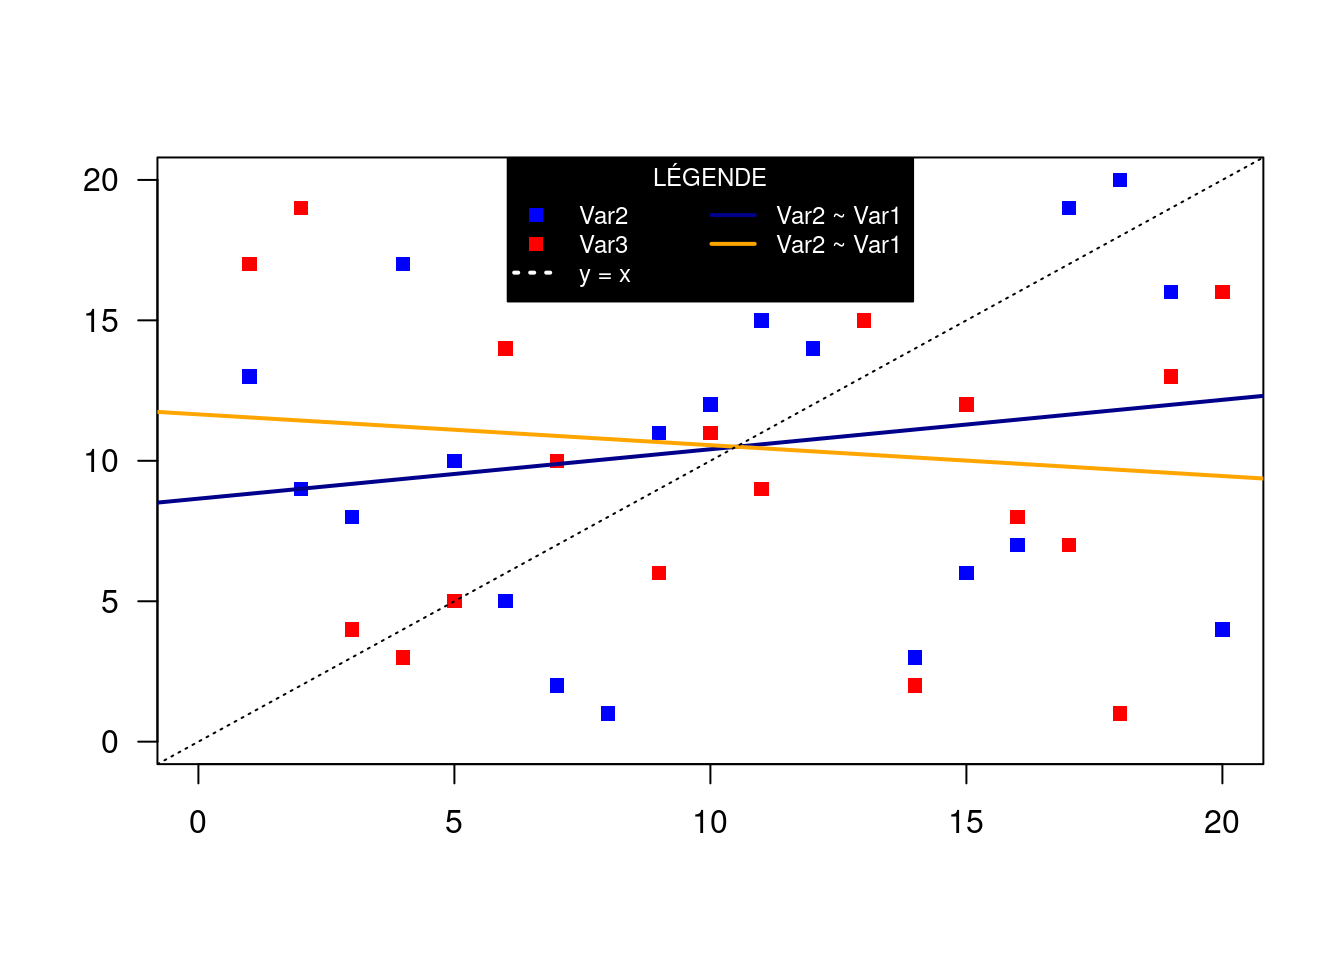
\includegraphics[width=.6\linewidth]{visualiseR_files/figure-latex/unnamed-chunk-33-1} \end{center}

\hypertarget{ajout-dun-axe}{%
\subsection{Ajout d'un axe}\label{ajout-dun-axe}}

Regardons comment ajouter des axes à un graphe. Dans un premier temps, nous allons faire un plot vide et créer nous-même les axes avec la fonction \texttt{axis()}. Cette fonction accepte plusieurs arguments détaillés dans le tableau suivant.

\textbf{Argument} \& \textbf{Signification}

\begin{itemize}
\tightlist
\item
  \texttt{side} \& \textbf{1} (bas), \textbf{2} (gauche), \textbf{3} (haut), \textbf{4} (gauche)
\item
  \texttt{at} \& Coordonnées où placer la graduation
\item
  \texttt{labels} \& Étiquettes des graduations (même longueur que \texttt{at})
\item
  \texttt{pos} \& Coordonnée de position sur l'axe perpendiculaire
\item
  \texttt{tick} \& \textbf{TRUE} ou \textbf{FALSE} (l'axe et la graduation ne sont pas tracés)
\item
  \texttt{lty} \& Type de ligne de l'axe
\item
  \texttt{lwd} \& Épaisseur de ligne de l'axe
\item
  \texttt{lwd.ticks} \& Épaisseur de ligne de la graduation
\item
  \texttt{col} \& Couleur de l'axe
\item
  \texttt{col.ticks} \& Couleur de la graduation
\item
  \texttt{col.axis} \& Couleur des étiquettes
\end{itemize}

\begin{Shaded}
\begin{Highlighting}[]
\KeywordTok{plot0}\NormalTok{(}\DataTypeTok{xlim =} \KeywordTok{c}\NormalTok{(}\OperatorTok{-}\DecValTok{2}\NormalTok{, }\DecValTok{2}\NormalTok{), }\DataTypeTok{ylim =} \KeywordTok{c}\NormalTok{(}\OperatorTok{-}\DecValTok{2}\NormalTok{, }\DecValTok{2}\NormalTok{))}
\KeywordTok{title}\NormalTok{(}\DataTypeTok{main =} \StringTok{"Plot retravaillé"}\NormalTok{)}
\NormalTok{grad <-}\StringTok{ }\KeywordTok{seq}\NormalTok{(}\OperatorTok{-}\DecValTok{2}\NormalTok{, }\DecValTok{2}\NormalTok{, }\DataTypeTok{by =} \FloatTok{0.5}\NormalTok{)}
\KeywordTok{axis}\NormalTok{(}\DataTypeTok{side =} \DecValTok{1}\NormalTok{, }\DataTypeTok{at =}\NormalTok{ grad, }\DataTypeTok{labels =} \KeywordTok{format}\NormalTok{(grad), }\DataTypeTok{pos =} \DecValTok{-2}\NormalTok{)}
\KeywordTok{axis}\NormalTok{(}\DataTypeTok{side =} \DecValTok{2}\NormalTok{, }\DataTypeTok{at =}\NormalTok{ grad, }\DataTypeTok{labels =} \KeywordTok{format}\NormalTok{(grad), }\DataTypeTok{pos =} \DecValTok{-2}\NormalTok{, }\DataTypeTok{las =} \DecValTok{2}\NormalTok{)}
\KeywordTok{axis}\NormalTok{(}\DataTypeTok{side =} \DecValTok{1}\NormalTok{, }\DataTypeTok{at =} \KeywordTok{seq}\NormalTok{(}\OperatorTok{-}\FloatTok{1.75}\NormalTok{, }\FloatTok{1.75}\NormalTok{, }\DataTypeTok{by =} \FloatTok{0.5}\NormalTok{), }\DataTypeTok{pos =} \DecValTok{-2}\NormalTok{, }\DataTypeTok{tck =} \FloatTok{-0.01}\NormalTok{, }\DataTypeTok{labels =} \OtherTok{FALSE}\NormalTok{, }\DataTypeTok{lwd =} \DecValTok{-2}\NormalTok{, }\DataTypeTok{lwd.ticks =} \DecValTok{1}\NormalTok{)}
\KeywordTok{axis}\NormalTok{(}\DataTypeTok{side =} \DecValTok{2}\NormalTok{, }\DataTypeTok{at =} \KeywordTok{seq}\NormalTok{(}\OperatorTok{-}\FloatTok{1.75}\NormalTok{, }\FloatTok{1.75}\NormalTok{, }\DataTypeTok{by =} \FloatTok{0.5}\NormalTok{), }\DataTypeTok{pos =} \DecValTok{-2}\NormalTok{, }\DataTypeTok{tck =} \FloatTok{-0.01}\NormalTok{, }\DataTypeTok{labels =} \OtherTok{FALSE}\NormalTok{, }\DataTypeTok{lwd =} \DecValTok{-2}\NormalTok{, }\DataTypeTok{lwd.ticks =} \DecValTok{1}\NormalTok{)}
\KeywordTok{mtext}\NormalTok{(}\DataTypeTok{side =} \DecValTok{1}\NormalTok{, }\DataTypeTok{line =} \FloatTok{1.5}\NormalTok{, }\DataTypeTok{text =} \StringTok{"Axe des x"}\NormalTok{, }\DataTypeTok{font =} \DecValTok{2}\NormalTok{)}
\KeywordTok{mtext}\NormalTok{(}\DataTypeTok{side =} \DecValTok{2}\NormalTok{, }\DataTypeTok{line =} \FloatTok{2.5}\NormalTok{, }\DataTypeTok{text =} \StringTok{"Axe des y"}\NormalTok{, }\DataTypeTok{font =} \DecValTok{2}\NormalTok{, }\DataTypeTok{las =} \DecValTok{0}\NormalTok{)}
\end{Highlighting}
\end{Shaded}

\begin{center}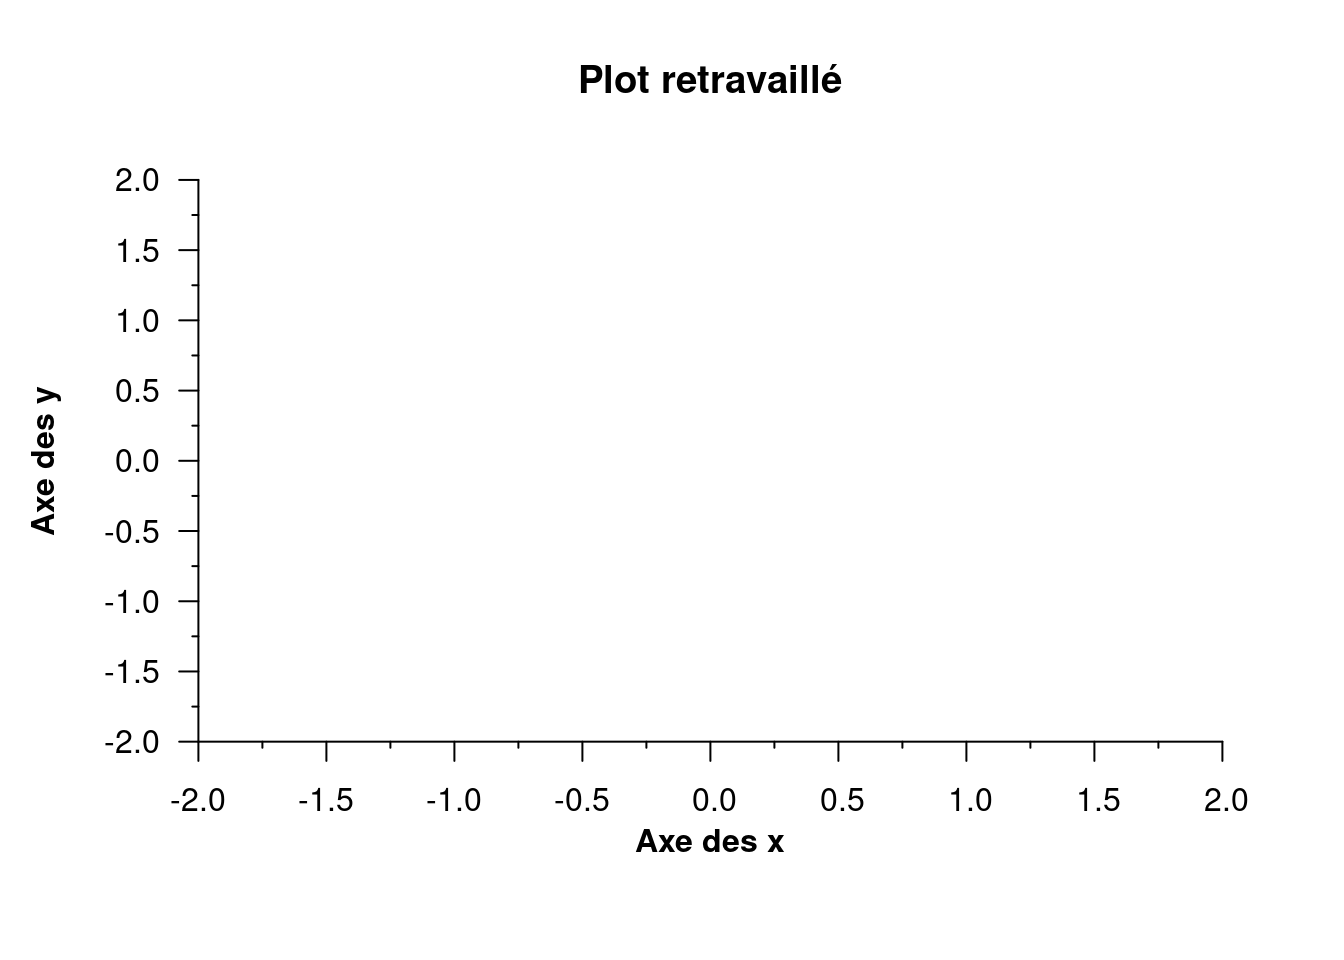
\includegraphics[width=.55\linewidth]{visualiseR_files/figure-latex/unnamed-chunk-34-1} \end{center}

Ici, nous avons défini une graduation secondaire dépourvue d'étiquette sur les axes avec une graduation plus fine. Nous avons également rajouté un nom aux axes avec la fonction \texttt{mtext()} puisque cette option n'est pas disponible dans la fonction \texttt{axis()}.

\hypertarget{ajout-dune-image}{%
\subsection{Ajout d'une image}\label{ajout-dune-image}}

Pour terminer ce chapitre, nous allons nous intéresser à l'inclusion d'une image dans un graphe. En effet, il peut être fort intéressant de pouvoir mettre une image quelconque sur un graphique. Par ex., sur une carte, il pourra s'agir de symboles divers permettant de figurer certains éléments caractéristiques (e.g.~parc de stationnement, hôtel, station météo, etc.) ou des repères (e.g.~nord géographique, etc.). Il pourra également s'agir du logo d'une institution, et bien d'autres.
La fonction \texttt{rasterImage()} du package \texttt{graphics} permet d'ajouter à un graphe existant une image sous forme matricielle. Il peut s'agir d'une image sous format \textbf{JPEG}, \textbf{PNG}, \textbf{GIF}, etc. Dans la suite, nous n'importerons que des images au format \textbf{PNG}. Pour ce faire, nous avons besoin de charger un package complémentaire, spécialement dédié à cette tâche : le package \texttt{png}.

\begin{Shaded}
\begin{Highlighting}[]
\CommentTok{## install.packages("png")}
\KeywordTok{library}\NormalTok{(png)}
\end{Highlighting}
\end{Shaded}

Nous avons développé une fonction, que nous avons appelée \texttt{plotimage()}, basée sur la fonction \texttt{rasterImage()}, qui permet d'importer dans un graphe n'importe quelle image au format \textbf{PNG}, \textbf{JPEG} ou \textbf{TIFF}. Cette fonction permet, soit d'ajouter l'image à un graphe existant, soit de créer un nouveau graphe avec cette image. De plus, elle permet de redimensionner l'image en conservant le rapport hauteur/largeur d'origine. Le tout s'adaptant aux dimensions du graphe. Enfin, cette fonction permet de positionner l'image soit en fournissant les coordonnées du centre, soit en utilisant des positions prédéfinies (e.g. ``center'', ``topleft'', etc.). Notons que tous les paramètres graphiques de la fonction \texttt{plot()} peuvent être modifiés (dans le cas où l'image est insérée dans une nouvelle fenêtre).

Commençons par définir cette fonction dans R.

\begin{Shaded}
\begin{Highlighting}[]
\NormalTok{plotimage <-}\StringTok{ }\ControlFlowTok{function}\NormalTok{(file, }\DataTypeTok{x =} \OtherTok{NULL}\NormalTok{, }\DataTypeTok{y =} \OtherTok{NULL}\NormalTok{, }\DataTypeTok{size =} \DecValTok{1}\NormalTok{, }\DataTypeTok{add =} \OtherTok{FALSE}\NormalTok{,}
\DataTypeTok{angle =} \DecValTok{0}\NormalTok{, }\DataTypeTok{pos =} \DecValTok{0}\NormalTok{, }\DataTypeTok{bg =} \StringTok{"lightgray"}\NormalTok{, ...)\{}
\ControlFlowTok{if}\NormalTok{ (}\KeywordTok{length}\NormalTok{(}\KeywordTok{grep}\NormalTok{(}\StringTok{".png"}\NormalTok{, file)) }\OperatorTok{>}\StringTok{ }\DecValTok{0}\NormalTok{)\{}
  \KeywordTok{require}\NormalTok{(}\StringTok{"png"}\NormalTok{)}
\NormalTok{  img <-}\StringTok{ }\KeywordTok{readPNG}\NormalTok{(file, }\DataTypeTok{native =} \OtherTok{TRUE}\NormalTok{)}
\NormalTok{\}}
\ControlFlowTok{if}\NormalTok{ (}\KeywordTok{length}\NormalTok{(}\KeywordTok{grep}\NormalTok{(}\StringTok{".tif"}\NormalTok{, file)) }\OperatorTok{>}\StringTok{ }\DecValTok{0}\NormalTok{)\{}
  \KeywordTok{require}\NormalTok{(}\StringTok{"tiff"}\NormalTok{)}
\NormalTok{  img <-}\StringTok{ }\KeywordTok{readTIFF}\NormalTok{(file, }\DataTypeTok{native =} \OtherTok{TRUE}\NormalTok{)}
\NormalTok{\}}
\ControlFlowTok{if}\NormalTok{ (}\KeywordTok{length}\NormalTok{(}\KeywordTok{grep}\NormalTok{(}\StringTok{".jp"}\NormalTok{, file)) }\OperatorTok{>}\StringTok{ }\DecValTok{0}\NormalTok{)\{}
  \KeywordTok{require}\NormalTok{(}\StringTok{"jpeg"}\NormalTok{)}
\NormalTok{  img <-}\StringTok{ }\KeywordTok{readJPEG}\NormalTok{(file, }\DataTypeTok{native =} \OtherTok{TRUE}\NormalTok{)}
\NormalTok{\}}
\NormalTok{res <-}\StringTok{ }\KeywordTok{dim}\NormalTok{(img)[}\DecValTok{2}\OperatorTok{:}\DecValTok{1}\NormalTok{]}
\ControlFlowTok{if}\NormalTok{ (add)\{}
\NormalTok{  xres <-}\StringTok{ }\KeywordTok{par}\NormalTok{()}\OperatorTok{$}\NormalTok{usr[}\DecValTok{2}\NormalTok{] }\OperatorTok{-}\StringTok{ }\KeywordTok{par}\NormalTok{()}\OperatorTok{$}\NormalTok{usr[}\DecValTok{1}\NormalTok{]}
\NormalTok{  yres <-}\StringTok{ }\KeywordTok{par}\NormalTok{()}\OperatorTok{$}\NormalTok{usr[}\DecValTok{4}\NormalTok{] }\OperatorTok{-}\StringTok{ }\KeywordTok{par}\NormalTok{()}\OperatorTok{$}\NormalTok{usr[}\DecValTok{3}\NormalTok{]}
\NormalTok{  res <-}\StringTok{ }\KeywordTok{c}\NormalTok{(xres, yres)}
\NormalTok{\} }\ControlFlowTok{else}\NormalTok{\{}
  \KeywordTok{par}\NormalTok{(}\DataTypeTok{mar =} \KeywordTok{c}\NormalTok{(}\DecValTok{1}\NormalTok{, }\DecValTok{1}\NormalTok{, }\DecValTok{1}\NormalTok{, }\DecValTok{1}\NormalTok{), }\DataTypeTok{bg =}\NormalTok{ bg, }\DataTypeTok{xaxs =} \StringTok{"i"}\NormalTok{, }\DataTypeTok{yaxs =} \StringTok{"i"}\NormalTok{)}
\NormalTok{  dims <-}\StringTok{ }\KeywordTok{c}\NormalTok{(}\DecValTok{0}\NormalTok{, }\KeywordTok{max}\NormalTok{(res))}
  \KeywordTok{plot}\NormalTok{(}\DecValTok{0}\NormalTok{, }\DataTypeTok{type =} \StringTok{"n"}\NormalTok{, }\DataTypeTok{axes =} \OtherTok{FALSE}\NormalTok{, }\DataTypeTok{xlim =}\NormalTok{ dims, }\DataTypeTok{ann =} \OtherTok{FALSE}\NormalTok{,}
  \DataTypeTok{ylim =}\NormalTok{ dims, ...)}
\NormalTok{\}}
\ControlFlowTok{if}\NormalTok{ (}\KeywordTok{is.null}\NormalTok{(x) }\OperatorTok{&&}\StringTok{ }\KeywordTok{is.null}\NormalTok{(y))\{}
\ControlFlowTok{if}\NormalTok{ (pos }\OperatorTok{==}\StringTok{ "center"} \OperatorTok{||}\StringTok{ }\NormalTok{pos }\OperatorTok{==}\StringTok{ }\DecValTok{0}\NormalTok{)\{}
\NormalTok{  x <-}\StringTok{ }\KeywordTok{par}\NormalTok{()}\OperatorTok{$}\NormalTok{usr[}\DecValTok{1}\NormalTok{]}\OperatorTok{+}\NormalTok{(}\KeywordTok{par}\NormalTok{()}\OperatorTok{$}\NormalTok{usr[}\DecValTok{2}\NormalTok{]}\OperatorTok{-}\KeywordTok{par}\NormalTok{()}\OperatorTok{$}\NormalTok{usr[}\DecValTok{1}\NormalTok{])}\OperatorTok{/}\DecValTok{2}
\NormalTok{  y <-}\StringTok{ }\KeywordTok{par}\NormalTok{()}\OperatorTok{$}\NormalTok{usr[}\DecValTok{3}\NormalTok{]}\OperatorTok{+}\NormalTok{(}\KeywordTok{par}\NormalTok{()}\OperatorTok{$}\NormalTok{usr[}\DecValTok{4}\NormalTok{]}\OperatorTok{-}\KeywordTok{par}\NormalTok{()}\OperatorTok{$}\NormalTok{usr[}\DecValTok{3}\NormalTok{])}\OperatorTok{/}\DecValTok{2}
\NormalTok{\}}
\ControlFlowTok{if}\NormalTok{ (pos }\OperatorTok{==}\StringTok{ "bottom"} \OperatorTok{||}\StringTok{ }\NormalTok{pos }\OperatorTok{==}\StringTok{ }\DecValTok{1}\NormalTok{)\{}
\NormalTok{  x <-}\StringTok{ }\KeywordTok{par}\NormalTok{()}\OperatorTok{$}\NormalTok{usr[}\DecValTok{1}\NormalTok{]}\OperatorTok{+}\NormalTok{(}\KeywordTok{par}\NormalTok{()}\OperatorTok{$}\NormalTok{usr[}\DecValTok{2}\NormalTok{]}\OperatorTok{-}\KeywordTok{par}\NormalTok{()}\OperatorTok{$}\NormalTok{usr[}\DecValTok{1}\NormalTok{])}\OperatorTok{/}\DecValTok{2}
\NormalTok{  y <-}\StringTok{ }\KeywordTok{par}\NormalTok{()}\OperatorTok{$}\NormalTok{usr[}\DecValTok{3}\NormalTok{]}\OperatorTok{+}\NormalTok{res[}\DecValTok{2}\NormalTok{]}\OperatorTok{*}\NormalTok{size}\OperatorTok{/}\DecValTok{2}
\NormalTok{\}}
\ControlFlowTok{if}\NormalTok{ (pos }\OperatorTok{==}\StringTok{ "left"} \OperatorTok{||}\StringTok{ }\NormalTok{pos }\OperatorTok{==}\StringTok{ }\DecValTok{2}\NormalTok{)\{}
\NormalTok{  x <-}\StringTok{ }\KeywordTok{par}\NormalTok{()}\OperatorTok{$}\NormalTok{usr[}\DecValTok{1}\NormalTok{]}\OperatorTok{+}\NormalTok{res[}\DecValTok{1}\NormalTok{]}\OperatorTok{*}\NormalTok{size}\OperatorTok{/}\DecValTok{2}
\NormalTok{  y <-}\StringTok{ }\KeywordTok{par}\NormalTok{()}\OperatorTok{$}\NormalTok{usr[}\DecValTok{3}\NormalTok{]}\OperatorTok{+}\NormalTok{(}\KeywordTok{par}\NormalTok{()}\OperatorTok{$}\NormalTok{usr[}\DecValTok{4}\NormalTok{]}\OperatorTok{-}\KeywordTok{par}\NormalTok{()}\OperatorTok{$}\NormalTok{usr[}\DecValTok{3}\NormalTok{])}\OperatorTok{/}\DecValTok{2}
\NormalTok{\}}
\ControlFlowTok{if}\NormalTok{ (pos }\OperatorTok{==}\StringTok{ "top"} \OperatorTok{||}\StringTok{ }\NormalTok{pos }\OperatorTok{==}\StringTok{ }\DecValTok{3}\NormalTok{)\{}
\NormalTok{  x <-}\StringTok{ }\KeywordTok{par}\NormalTok{()}\OperatorTok{$}\NormalTok{usr[}\DecValTok{1}\NormalTok{]}\OperatorTok{+}\NormalTok{(}\KeywordTok{par}\NormalTok{()}\OperatorTok{$}\NormalTok{usr[}\DecValTok{2}\NormalTok{]}\OperatorTok{-}\KeywordTok{par}\NormalTok{()}\OperatorTok{$}\NormalTok{usr[}\DecValTok{1}\NormalTok{])}\OperatorTok{/}\DecValTok{2}
\NormalTok{  y <-}\StringTok{ }\KeywordTok{par}\NormalTok{()}\OperatorTok{$}\NormalTok{usr[}\DecValTok{4}\NormalTok{]}\OperatorTok{-}\NormalTok{res[}\DecValTok{2}\NormalTok{]}\OperatorTok{*}\NormalTok{size}\OperatorTok{/}\DecValTok{2}
\NormalTok{\}}
\ControlFlowTok{if}\NormalTok{ (pos }\OperatorTok{==}\StringTok{ "right"} \OperatorTok{||}\StringTok{ }\NormalTok{pos }\OperatorTok{==}\StringTok{ }\DecValTok{4}\NormalTok{)\{}
\NormalTok{  x <-}\StringTok{ }\KeywordTok{par}\NormalTok{()}\OperatorTok{$}\NormalTok{usr[}\DecValTok{2}\NormalTok{]}\OperatorTok{-}\NormalTok{res[}\DecValTok{1}\NormalTok{]}\OperatorTok{*}\NormalTok{size}\OperatorTok{/}\DecValTok{2}
\NormalTok{  y <-}\StringTok{ }\KeywordTok{par}\NormalTok{()}\OperatorTok{$}\NormalTok{usr[}\DecValTok{3}\NormalTok{]}\OperatorTok{+}\NormalTok{(}\KeywordTok{par}\NormalTok{()}\OperatorTok{$}\NormalTok{usr[}\DecValTok{4}\NormalTok{]}\OperatorTok{-}\KeywordTok{par}\NormalTok{()}\OperatorTok{$}\NormalTok{usr[}\DecValTok{3}\NormalTok{])}\OperatorTok{/}\DecValTok{2}
\NormalTok{\}}
\ControlFlowTok{if}\NormalTok{ (pos }\OperatorTok{==}\StringTok{ "bottomleft"} \OperatorTok{||}\StringTok{ }\NormalTok{pos }\OperatorTok{==}\StringTok{ }\DecValTok{5}\NormalTok{)\{}
\NormalTok{x <-}\StringTok{ }\KeywordTok{par}\NormalTok{()}\OperatorTok{$}\NormalTok{usr[}\DecValTok{1}\NormalTok{]}\OperatorTok{+}\NormalTok{res[}\DecValTok{1}\NormalTok{]}\OperatorTok{*}\NormalTok{size}\OperatorTok{/}\DecValTok{2}
\NormalTok{y <-}\StringTok{ }\KeywordTok{par}\NormalTok{()}\OperatorTok{$}\NormalTok{usr[}\DecValTok{3}\NormalTok{]}\OperatorTok{+}\NormalTok{res[}\DecValTok{2}\NormalTok{]}\OperatorTok{*}\NormalTok{size}\OperatorTok{/}\DecValTok{2}
\NormalTok{\}}
\ControlFlowTok{if}\NormalTok{ (pos }\OperatorTok{==}\StringTok{ "topleft"} \OperatorTok{||}\StringTok{ }\NormalTok{pos }\OperatorTok{==}\StringTok{ }\DecValTok{6}\NormalTok{)\{}
\NormalTok{  x <-}\StringTok{ }\KeywordTok{par}\NormalTok{()}\OperatorTok{$}\NormalTok{usr[}\DecValTok{1}\NormalTok{]}\OperatorTok{+}\NormalTok{res[}\DecValTok{1}\NormalTok{]}\OperatorTok{*}\NormalTok{size}\OperatorTok{/}\DecValTok{2}
\NormalTok{  y <-}\StringTok{ }\KeywordTok{par}\NormalTok{()}\OperatorTok{$}\NormalTok{usr[}\DecValTok{4}\NormalTok{]}\OperatorTok{-}\NormalTok{res[}\DecValTok{2}\NormalTok{]}\OperatorTok{*}\NormalTok{size}\OperatorTok{/}\DecValTok{2}
\NormalTok{\}}
\ControlFlowTok{if}\NormalTok{ (pos }\OperatorTok{==}\StringTok{ "topright"} \OperatorTok{||}\StringTok{ }\NormalTok{pos }\OperatorTok{==}\StringTok{ }\DecValTok{7}\NormalTok{)\{}
\NormalTok{  x <-}\StringTok{ }\KeywordTok{par}\NormalTok{()}\OperatorTok{$}\NormalTok{usr[}\DecValTok{2}\NormalTok{]}\OperatorTok{-}\NormalTok{res[}\DecValTok{1}\NormalTok{]}\OperatorTok{*}\NormalTok{size}\OperatorTok{/}\DecValTok{2}
\NormalTok{  y <-}\StringTok{ }\KeywordTok{par}\NormalTok{()}\OperatorTok{$}\NormalTok{usr[}\DecValTok{4}\NormalTok{]}\OperatorTok{-}\NormalTok{res[}\DecValTok{2}\NormalTok{]}\OperatorTok{*}\NormalTok{size}\OperatorTok{/}\DecValTok{2}
\NormalTok{\}}
\ControlFlowTok{if}\NormalTok{ (pos }\OperatorTok{==}\StringTok{ "bottomright"} \OperatorTok{||}\StringTok{ }\NormalTok{pos }\OperatorTok{==}\StringTok{ }\DecValTok{8}\NormalTok{)\{}
\NormalTok{  x <-}\StringTok{ }\KeywordTok{par}\NormalTok{()}\OperatorTok{$}\NormalTok{usr[}\DecValTok{2}\NormalTok{]}\OperatorTok{-}\NormalTok{res[}\DecValTok{1}\NormalTok{]}\OperatorTok{*}\NormalTok{size}\OperatorTok{/}\DecValTok{2}
\NormalTok{  y <-}\StringTok{ }\KeywordTok{par}\NormalTok{()}\OperatorTok{$}\NormalTok{usr[}\DecValTok{3}\NormalTok{]}\OperatorTok{+}\NormalTok{res[}\DecValTok{2}\NormalTok{]}\OperatorTok{*}\NormalTok{size}\OperatorTok{/}\DecValTok{2}
\NormalTok{\}}
\NormalTok{\}}
\NormalTok{xx <-}\StringTok{ }\NormalTok{res[}\DecValTok{1}\NormalTok{]}\OperatorTok{*}\NormalTok{size}\OperatorTok{/}\DecValTok{2}
\NormalTok{yy <-}\StringTok{ }\NormalTok{res[}\DecValTok{2}\NormalTok{]}\OperatorTok{*}\NormalTok{size}\OperatorTok{/}\DecValTok{2}
\KeywordTok{rasterImage}\NormalTok{(img, x}\OperatorTok{-}\NormalTok{xx, y}\OperatorTok{-}\NormalTok{yy, x}\OperatorTok{+}\NormalTok{xx, y}\OperatorTok{+}\NormalTok{yy, }\DataTypeTok{angle =}\NormalTok{ angle)}
\NormalTok{\}}
\end{Highlighting}
\end{Shaded}

Voici les différents arguments possibles pour cette fonction.

\textbf{Argument} \& \textbf{Signification}\textbackslash{}
- \texttt{file} \& Nom de l'image à ouvrir (avec extension png)
- \texttt{x} \& Coordonnée en x du centre de l'image
- \texttt{y} \& Coordonnée en y du centre de l'image
- \texttt{pos} \& Position prédéfinie. Alternative à x et y. (voir la fonction \texttt{legend()})
- \texttt{size} \& Coefficient réducteur de l'image (entre 0 et 1)
- \texttt{angle} \& Degré de rotation de l'image (entre 0 et 360)
- \texttt{bg} \& Couleur du fond de la figure
- \texttt{add} \& \textbf{TRUE} ou \textbf{FALSE}
- \texttt{...} \& Autres paramètres graphiques de la fonction \texttt{plot()}

Le site Web \url{http://www.flaticon.com} permet de télécharger plus de 60 000 icônes gratuitement à différentes résolutions et sous différents formats. Les images suivantes sont issues de ce site. Merci aux auteurs !

\begin{Shaded}
\begin{Highlighting}[]
\CommentTok{# plotimage(file = "img/chap5/icon4.png", add = FALSE)}
\end{Highlighting}
\end{Shaded}

Regardons les différents placements par défaut.

\begin{Shaded}
\begin{Highlighting}[]
\KeywordTok{par}\NormalTok{(}\DataTypeTok{mfrow =} \KeywordTok{c}\NormalTok{(}\DecValTok{3}\NormalTok{, }\DecValTok{3}\NormalTok{))}
\ControlFlowTok{for}\NormalTok{ (i }\ControlFlowTok{in} \DecValTok{0} \OperatorTok{:}\StringTok{ }\DecValTok{8}\NormalTok{)\{}
\KeywordTok{plotimage}\NormalTok{(}\StringTok{"./icon8.png"}\NormalTok{, }\DataTypeTok{size =} \FloatTok{0.25}\NormalTok{, }\DataTypeTok{pos =}\NormalTok{ i)}
\KeywordTok{box}\NormalTok{(}\StringTok{"figure"}\NormalTok{)}
\NormalTok{\}}
\end{Highlighting}
\end{Shaded}

\begin{Shaded}
\begin{Highlighting}[]
\KeywordTok{plot}\NormalTok{(}\DecValTok{0}\NormalTok{, }\DataTypeTok{type =} \StringTok{"n"}\NormalTok{, }\DataTypeTok{axes =} \OtherTok{FALSE}\NormalTok{, }\DataTypeTok{ann =} \OtherTok{FALSE}\NormalTok{)}
\ControlFlowTok{for}\NormalTok{ (i }\ControlFlowTok{in} \DecValTok{0} \OperatorTok{:}\StringTok{ }\DecValTok{8}\NormalTok{)}
\KeywordTok{plotimage}\NormalTok{(}\StringTok{"./icon6.png"}\NormalTok{, }\DataTypeTok{size =} \FloatTok{0.25}\NormalTok{, }\DataTypeTok{pos =}\NormalTok{ i, }\DataTypeTok{add =} \OtherTok{TRUE}\NormalTok{)}
\KeywordTok{box}\NormalTok{(}\StringTok{"figure"}\NormalTok{)}
\end{Highlighting}
\end{Shaded}

Pour terminer, regardons l'impact de l'angle en superposant la même image tous les 45 degrés. Les formes résultantes n'étaient pas du tout prévu par les auteurs. Et, le résultat est très surprenant et esthétique. De la pure sérendipité !!!

\begin{Shaded}
\begin{Highlighting}[]
\KeywordTok{plot0}\NormalTok{(}\DataTypeTok{xlim =} \KeywordTok{c}\NormalTok{(}\OperatorTok{-}\DecValTok{1}\NormalTok{, }\DecValTok{1}\NormalTok{), }\DataTypeTok{ylim =} \KeywordTok{c}\NormalTok{(}\OperatorTok{-}\DecValTok{1}\NormalTok{, }\DecValTok{1}\NormalTok{), }\DataTypeTok{xaxs =} \StringTok{"i"}\NormalTok{, }\DataTypeTok{yaxs =} \StringTok{"i"}\NormalTok{)}
\ControlFlowTok{for}\NormalTok{ (i }\ControlFlowTok{in} \KeywordTok{seq}\NormalTok{(}\DecValTok{0}\NormalTok{, }\DecValTok{360}\NormalTok{, }\DecValTok{45}\NormalTok{))\{}
\KeywordTok{plotimage}\NormalTok{(}\StringTok{"./icon2.png"}\NormalTok{, }\DataTypeTok{size =} \FloatTok{0.25}\NormalTok{, }\DataTypeTok{add =} \OtherTok{TRUE}\NormalTok{, }\DataTypeTok{angle =}\NormalTok{ i, }\DataTypeTok{x =} \FloatTok{.25}\NormalTok{, }\DataTypeTok{y =} \FloatTok{.25}\NormalTok{)}
\NormalTok{\}}
\KeywordTok{plotimage}\NormalTok{(}\StringTok{"./icon2.png"}\NormalTok{, }\DataTypeTok{size =} \FloatTok{0.2}\NormalTok{, }\DataTypeTok{add =} \OtherTok{TRUE}\NormalTok{, }\DataTypeTok{pos =} \DecValTok{7}\NormalTok{)}
\KeywordTok{box}\NormalTok{(}\StringTok{"figure"}\NormalTok{)}
\end{Highlighting}
\end{Shaded}

Un petit dernier, parce qu'on aime ça.

\hypertarget{graphiques-classiques}{%
\section{Graphiques classiques}\label{graphiques-classiques}}

Regardons tout d'abord quelques fonctions permettant de réaliser des graphiques parmi les plus communs dans la recherche scientifique. Sous R, de tels graphes sont réalisés avec des \emph{High-level plotting functions}, c.-à.d. que l'appel à ces fonctions effacera le précédent contenu du périphérique graphique actif. Mais, nous verrons dans le dernier chapitre qu'il est possible de contourner cet obstacle. On opposera ces fonctions aux \emph{Low-level plotting functions} qui elles, permettront d'ajouter des éléments à un graphique pré-existant. C'est l'objet du chapitre suivant.

\hypertarget{diagramme-de-dispersion}{%
\subsection{Diagramme de dispersion}\label{diagramme-de-dispersion}}

Il s'agit d'un graphe classique permettant de représenter deux variables continues l'une en fonction de l'autre dans un nuage de points. Nous allons réutiliser pour cela la fonction \texttt{plot()}.
Créons une variable contenant une série de valeurs allant de 1 à 20.

\begin{Shaded}
\begin{Highlighting}[]
\NormalTok{(var1 <-}\StringTok{ }\KeywordTok{seq}\NormalTok{(}\DataTypeTok{from =} \DecValTok{1}\NormalTok{, }\DataTypeTok{to =} \DecValTok{20}\NormalTok{, }\DataTypeTok{by =} \DecValTok{1}\NormalTok{))}
\CommentTok{#>  [1]  1  2  3  4  5  6  7  8  9 10 11 12 13 14 15 16 17 18 19 20}
\end{Highlighting}
\end{Shaded}

Remarque : les parenthèses permettent d'afficher dans la console le résultat de l'assignation. Générons une seconde variable avec 20 valeurs tirées aléatoirement selon une distribution normale de moyenne 0 et d'écart-type 1.

\begin{Shaded}
\begin{Highlighting}[]
\NormalTok{(var2 <-}\StringTok{ }\KeywordTok{rnorm}\NormalTok{(}\DataTypeTok{n =} \DecValTok{20}\NormalTok{, }\DataTypeTok{mean =} \DecValTok{0}\NormalTok{, }\DataTypeTok{sd =} \DecValTok{1}\NormalTok{))}
\CommentTok{#>  [1]  0.89689312  0.30913630  1.28111734 -1.31379564 -1.42625186  0.79876349}
\CommentTok{#>  [7] -0.44574525 -0.03844782 -0.41255644 -0.82786204  0.40196226  1.18768404}
\CommentTok{#> [13]  1.32915936  0.79981119  1.69035185  0.34798365 -0.72282932 -1.50359497}
\CommentTok{#> [19]  0.38816553  0.36377291}
\end{Highlighting}
\end{Shaded}

Représentons maintenant le nuage de points (\emph{scatterplot}) formés des valeurs de \textbf{var1} et \textbf{var2}.

\begin{Shaded}
\begin{Highlighting}[]
\KeywordTok{plot}\NormalTok{(}\DataTypeTok{x =}\NormalTok{ var1, }\DataTypeTok{y =}\NormalTok{ var2)}
\end{Highlighting}
\end{Shaded}

\begin{center}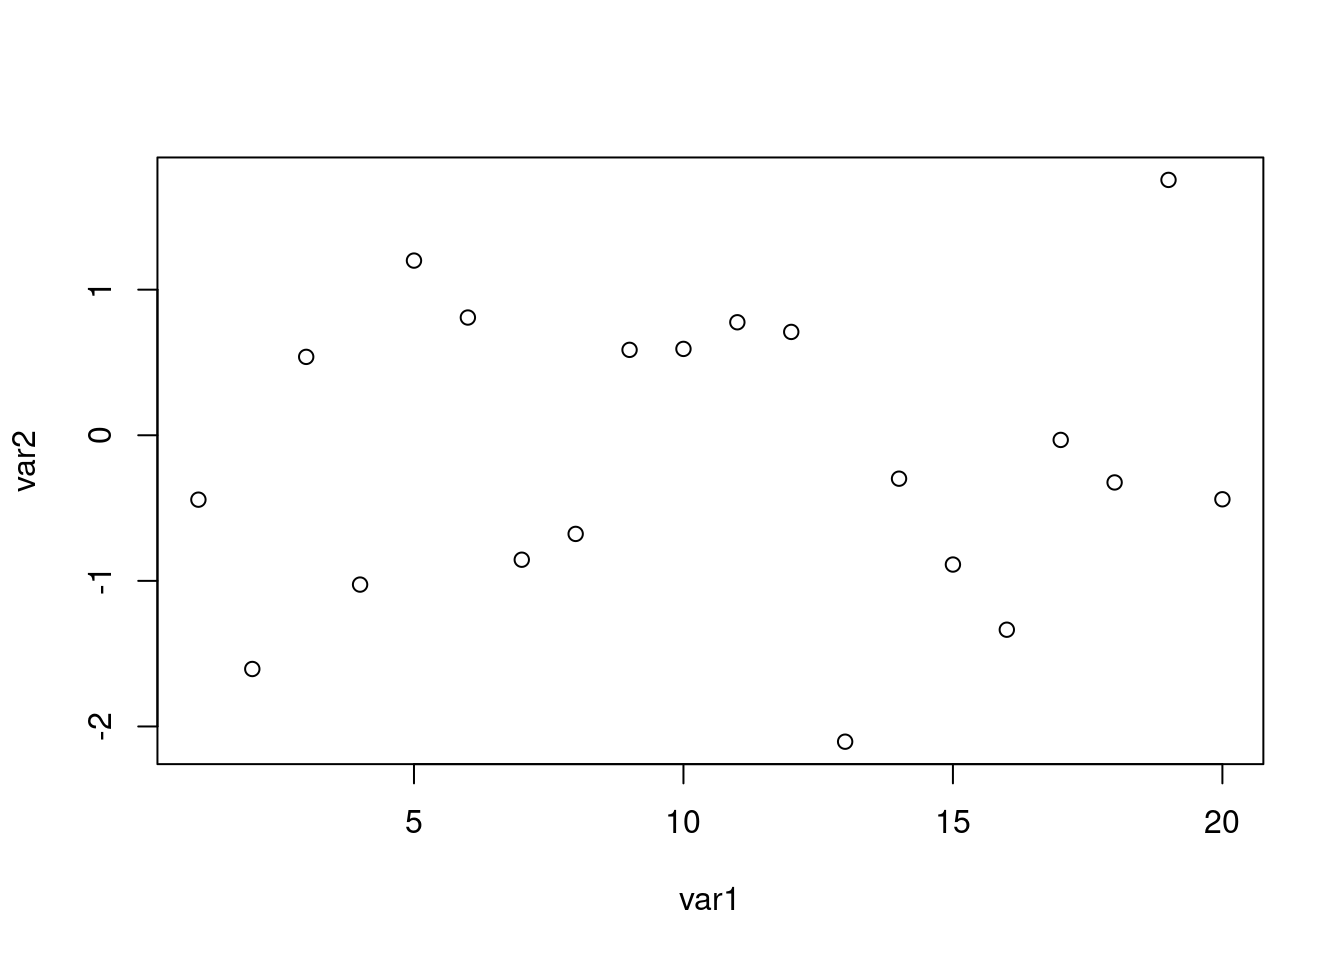
\includegraphics[width=.55\linewidth]{visualiseR_files/figure-latex/unnamed-chunk-44-1} \end{center}

Anticipons légèrement sur les chapitres suivants et intéressons-nous à l'argument \texttt{type} de la fonction \texttt{plot()}. Celui-ci permet de représenter les données de différentes manières : nuage de points, barres verticales, lignes, etc.
\{ll\}

\textbf{Valeur} \& \textbf{Représentation}\textbackslash{}

\begin{itemize}
\tightlist
\item
  \texttt{type = 'p'} \& Points
\item
  \texttt{type = 'l'} \& Lignes reliées
\item
  \texttt{type = 'c'} \& Lignes non reliées
\item
  \texttt{type = 'b'} \& Points et lignes non reliées
\item
  \texttt{type = 'o'} \& Points et lignes reliées
\item
  \texttt{type = 'h'} \& Barres verticales
\item
  \texttt{type = 's'} \& Plateau puis pente
\item
  \texttt{type = 'S'} \& Pente puis creux
\item
  \texttt{type = 'n'} \& Aucun symbole
\end{itemize}

Afin de bien comprendre les différences, partitionnons la fenêtre graphique en neuf régions distinctes (trois lignes et trois colonnes), chacune destinée à recevoir un plot spécifique avec une valeur différente pour l'argument \texttt{type}. Nous allons donc modifier le paramètre graphique \texttt{mfrow} de l'objet \texttt{par()}. Avec cet argument, les régions graphiques seront remplies en lignes.

Nous allons également rajouter un titre à chaque graphique qui contient la valeur de l'argument \texttt{type}. L'argument \texttt{main} permet de rajouter un titre principal à un graphe qui se positionnera en haut du graphique.

\begin{Shaded}
\begin{Highlighting}[]
\KeywordTok{par}\NormalTok{(}\DataTypeTok{mfrow =} \KeywordTok{c}\NormalTok{(}\DecValTok{3}\NormalTok{, }\DecValTok{3}\NormalTok{))}
\KeywordTok{plot}\NormalTok{(var1, var2, }\DataTypeTok{type =} \StringTok{"p"}\NormalTok{, }\DataTypeTok{main =} \StringTok{"Type = p"}\NormalTok{)}
\KeywordTok{plot}\NormalTok{(var1, var2, }\DataTypeTok{type =} \StringTok{"l"}\NormalTok{, }\DataTypeTok{main =} \StringTok{"Type = l"}\NormalTok{)}
\KeywordTok{plot}\NormalTok{(var1, var2, }\DataTypeTok{type =} \StringTok{"b"}\NormalTok{, }\DataTypeTok{main =} \StringTok{"Type = b"}\NormalTok{)}
\KeywordTok{plot}\NormalTok{(var1, var2, }\DataTypeTok{type =} \StringTok{"o"}\NormalTok{, }\DataTypeTok{main =} \StringTok{"Type = o"}\NormalTok{)}
\KeywordTok{plot}\NormalTok{(var1, var2, }\DataTypeTok{type =} \StringTok{"c"}\NormalTok{, }\DataTypeTok{main =} \StringTok{"Type = c"}\NormalTok{)}
\KeywordTok{plot}\NormalTok{(var1, var2, }\DataTypeTok{type =} \StringTok{"h"}\NormalTok{, }\DataTypeTok{main =} \StringTok{"Type = h"}\NormalTok{)}
\KeywordTok{plot}\NormalTok{(var1, var2, }\DataTypeTok{type =} \StringTok{"s"}\NormalTok{, }\DataTypeTok{main =} \StringTok{"Type = s"}\NormalTok{)}
\KeywordTok{plot}\NormalTok{(var1, var2, }\DataTypeTok{type =} \StringTok{"S"}\NormalTok{, }\DataTypeTok{main =} \StringTok{"Type = S"}\NormalTok{)}
\KeywordTok{plot}\NormalTok{(var1, var2, }\DataTypeTok{type =} \StringTok{"n"}\NormalTok{, }\DataTypeTok{main =} \StringTok{"Type = n"}\NormalTok{)}
\end{Highlighting}
\end{Shaded}

\begin{center}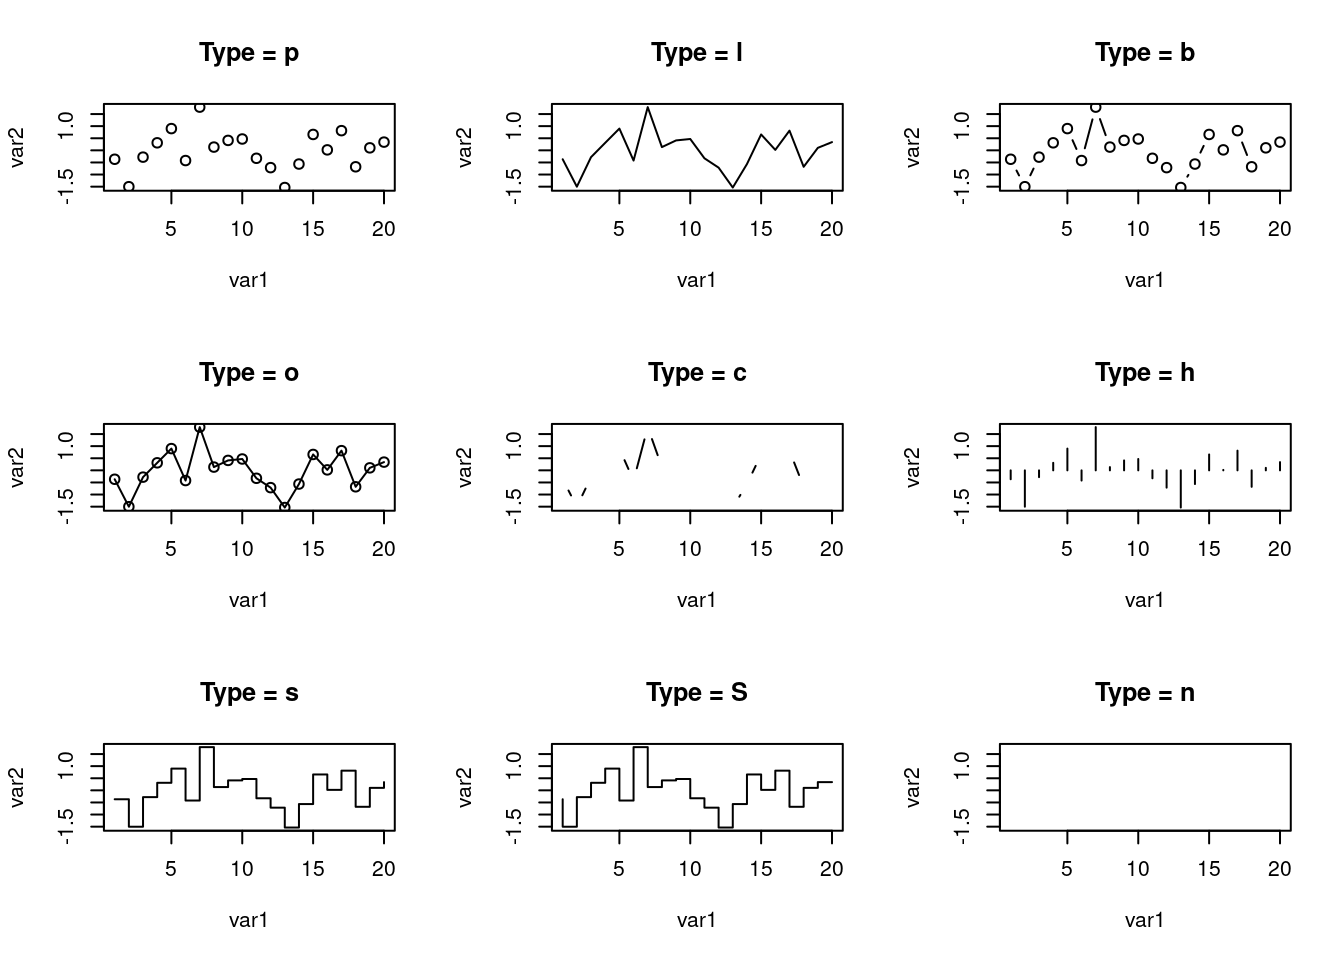
\includegraphics{visualiseR_files/figure-latex/unnamed-chunk-45-1} \end{center}

La fonction \texttt{plot()} offre de nombreux autres arguments qu'il est possible de modifier. C'est en partie ce que nous verrons tout au long de ce document, puisque cet enseignement met essentiellement l'accent sur cette fonction.

\hypertarget{bouxeete-uxe0-moustaches}{%
\subsection{Boîte à moustaches}\label{bouxeete-uxe0-moustaches}}

La boîte à moustaches est une représentation graphique très utile en
statistiques, puisqu'elle permet de résumer les caractéristiques de position
(médiane, 1\textsuperscript{er} et 3\textsuperscript{ème} quartiles, minimum et maximum) d'une variable
quantitative. Sous R, la fonction utilisée sera \texttt{boxplot()}.

\begin{Shaded}
\begin{Highlighting}[]
\KeywordTok{boxplot}\NormalTok{(var1, var2)}
\end{Highlighting}
\end{Shaded}

\begin{center}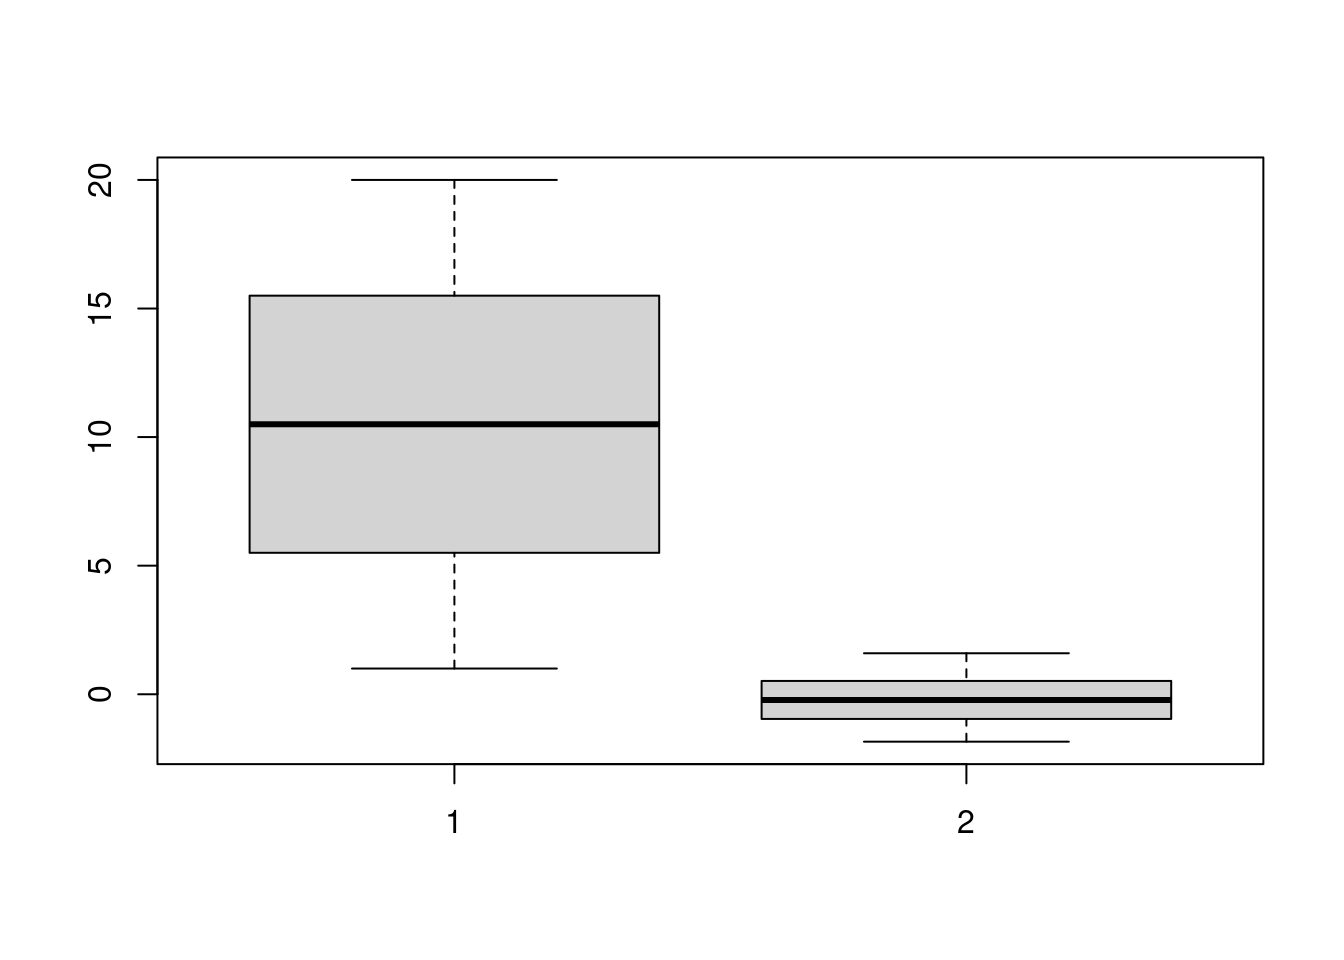
\includegraphics[width=.55\linewidth]{visualiseR_files/figure-latex/unnamed-chunk-46-1} \end{center}

Cette fonction s'applique sur des vecteurs, mais aussi sur des data frames. Elle possède de nombreux arguments. Par exemple, le tableau suivant liste les paramètres les plus courants.
\{ll\}

\textbf{Argument} \& \textbf{Signification}:

\begin{itemize}
\tightlist
\item
  \texttt{width} \& Largeur des boîtes (valeurs à fournir)
\item
  \texttt{varwidth} \& Largeur des boîtes (proportionnelle au n)
\item
  \texttt{outline} \& Suppression des outliers
\item
  \texttt{horizontal} \& Vertical ou horizontal
\item
  \texttt{add} \& Rajout d'une boîte
\item
  \texttt{at} \& Coordonnée en x de la nouvelle boîte
\end{itemize}

L'argument \texttt{plot} mis à la valeur \textbf{FALSE} n'affiche pas de boîte à moustaches, mais retourne les différentes statistiques associées sous la console. Par exemple:

\begin{Shaded}
\begin{Highlighting}[]
\KeywordTok{boxplot}\NormalTok{(var2, }\DataTypeTok{plot =} \OtherTok{FALSE}\NormalTok{)}
\CommentTok{#> $stats}
\CommentTok{#>            [,1]}
\CommentTok{#> [1,] -1.5035950}
\CommentTok{#> [2,] -0.5842873}
\CommentTok{#> [3,]  0.3558783}
\CommentTok{#> [4,]  0.8483522}
\CommentTok{#> [5,]  1.6903518}
\CommentTok{#> }
\CommentTok{#> $n}
\CommentTok{#> [1] 20}
\CommentTok{#> }
\CommentTok{#> $conf}
\CommentTok{#>            [,1]}
\CommentTok{#> [1,] -0.1502714}
\CommentTok{#> [2,]  0.8620280}
\CommentTok{#> }
\CommentTok{#> $out}
\CommentTok{#> numeric(0)}
\CommentTok{#> }
\CommentTok{#> $group}
\CommentTok{#> numeric(0)}
\CommentTok{#> }
\CommentTok{#> $names}
\CommentTok{#> [1] "1"}
\end{Highlighting}
\end{Shaded}

\hypertarget{diagramme-en-buxe2tons}{%
\subsection{Diagramme en bâtons}\label{diagramme-en-buxe2tons}}

Ce type de représentation est utile pour visualiser des données discrètes ou catégoriques. Chaque modalité de la variable catégorique (ou discrète) sera représentée par une barre verticale (ou horizontale) dont la longueur sera proportionnelle à son effectif (relatif ou absolu) parmi l'ensemble des modalités. Sous R, on réalise un tel graphique avec la fonction \texttt{barplot()}.
Créons tout d'abord un vecteur contenant six modalités (chaînes de caractères).

\begin{Shaded}
\begin{Highlighting}[]
\NormalTok{(nom <-}\StringTok{ }\KeywordTok{c}\NormalTok{(}\StringTok{"Vert"}\NormalTok{, }\StringTok{"Jaune"}\NormalTok{, }\StringTok{"Rouge"}\NormalTok{, }\StringTok{"Blanc"}\NormalTok{, }\StringTok{"Bleu"}\NormalTok{, }\StringTok{"Noir"}\NormalTok{))}
\CommentTok{#> [1] "Vert"  "Jaune" "Rouge" "Blanc" "Bleu"  "Noir"}
\end{Highlighting}
\end{Shaded}

Maintenant, nous allons tirer aléatoirement 1000 valeurs (avec remise donc) dans ce vecteur afin que chaque couleur soit présente plusieurs fois.

\begin{Shaded}
\begin{Highlighting}[]
\NormalTok{echn <-}\StringTok{ }\KeywordTok{sample}\NormalTok{(}\DataTypeTok{x =}\NormalTok{ nom, }\DataTypeTok{size =} \DecValTok{1000}\NormalTok{, }\DataTypeTok{replace =} \OtherTok{TRUE}\NormalTok{)}
\NormalTok{echn[}\DecValTok{1}\OperatorTok{:}\DecValTok{20}\NormalTok{]}
\CommentTok{#>  [1] "Noir"  "Noir"  "Rouge" "Bleu"  "Jaune" "Bleu"  "Bleu"  "Vert"  "Rouge"}
\CommentTok{#> [10] "Blanc" "Bleu"  "Vert"  "Bleu"  "Noir"  "Rouge" "Noir"  "Rouge" "Noir" }
\CommentTok{#> [19] "Noir"  "Blanc"}
\end{Highlighting}
\end{Shaded}

Comptons combien de fois se retrouve chaque modalité dans cette variable.

\begin{Shaded}
\begin{Highlighting}[]
\NormalTok{(var4 <-}\StringTok{ }\KeywordTok{table}\NormalTok{(echn))}
\CommentTok{#> echn}
\CommentTok{#> Blanc  Bleu Jaune  Noir Rouge  Vert }
\CommentTok{#>   175   166   165   178   161   155}
\end{Highlighting}
\end{Shaded}

Visualisons cette nouvelle variable catégorique.

\begin{Shaded}
\begin{Highlighting}[]
\KeywordTok{barplot}\NormalTok{(var4)}
\end{Highlighting}
\end{Shaded}

\begin{center}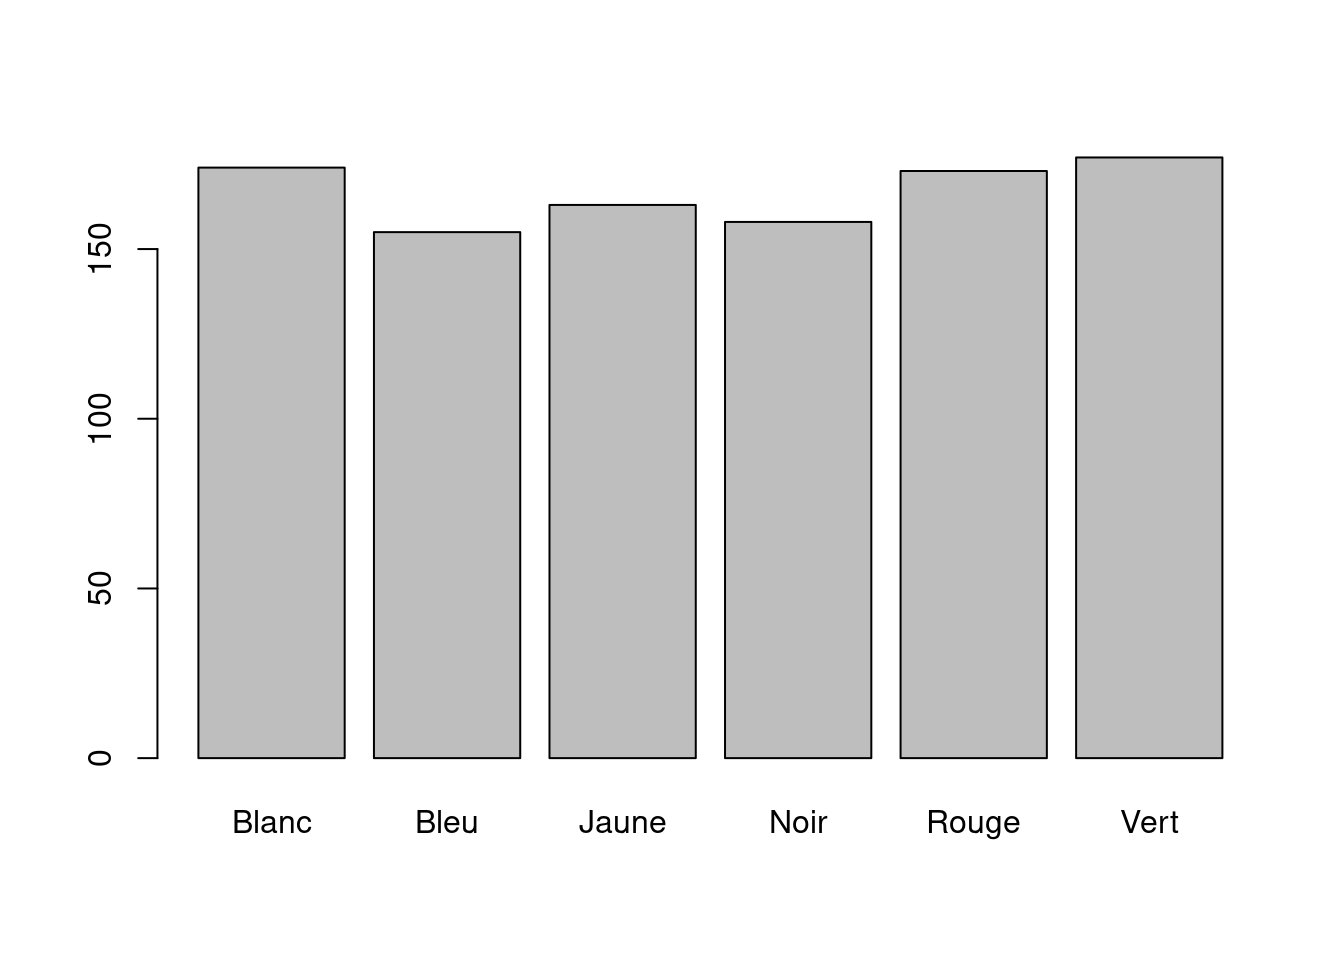
\includegraphics[width=0.6\linewidth]{visualiseR_files/figure-latex/unnamed-chunk-51-1} \end{center}

Nous pouvons également représenter cette même variable sous forme relative. Calculons la fréquence de chaque modalité et produisons un nouveau graphe.

\begin{Shaded}
\begin{Highlighting}[]
\NormalTok{(var5 <-}\StringTok{ }\NormalTok{var4}\OperatorTok{/}\KeywordTok{sum}\NormalTok{(var4))}
\CommentTok{#> echn}
\CommentTok{#> Blanc  Bleu Jaune  Noir Rouge  Vert }
\CommentTok{#> 0.175 0.166 0.165 0.178 0.161 0.155}
\end{Highlighting}
\end{Shaded}

Visuellement, rien ne changera, mis à part les valeurs portées sur l'axe des ordonnées. La fonction \texttt{barplot()} possède aussi de nombreux arguments. Nous vous invitons à consulter l'aide associée à cette fonction.

\begin{Shaded}
\begin{Highlighting}[]
\KeywordTok{help}\NormalTok{(barplot)}
\end{Highlighting}
\end{Shaded}

Il est possible de hachurer les rectangles plutôt que de leur associer une couleur. Pour ce faire, deux arguments doivent être spécifiés :
- \texttt{density} : nombre de hachures par pouce;
- \texttt{angle} : orientation des hachures dans le sens trigonométrique.
Par exemple,

\begin{Shaded}
\begin{Highlighting}[]
\KeywordTok{barplot}\NormalTok{(var4, }\DataTypeTok{density =} \KeywordTok{c}\NormalTok{(}\KeywordTok{rep}\NormalTok{(}\DecValTok{5}\NormalTok{, }\DecValTok{4}\NormalTok{), }\DecValTok{40}\NormalTok{, }\DecValTok{10}\NormalTok{), }\DataTypeTok{angle =} \KeywordTok{c}\NormalTok{(}\DecValTok{0}\NormalTok{, }\DecValTok{45}\NormalTok{, }\DecValTok{90}\NormalTok{, }\DecValTok{135}\NormalTok{))}
\end{Highlighting}
\end{Shaded}

\begin{center}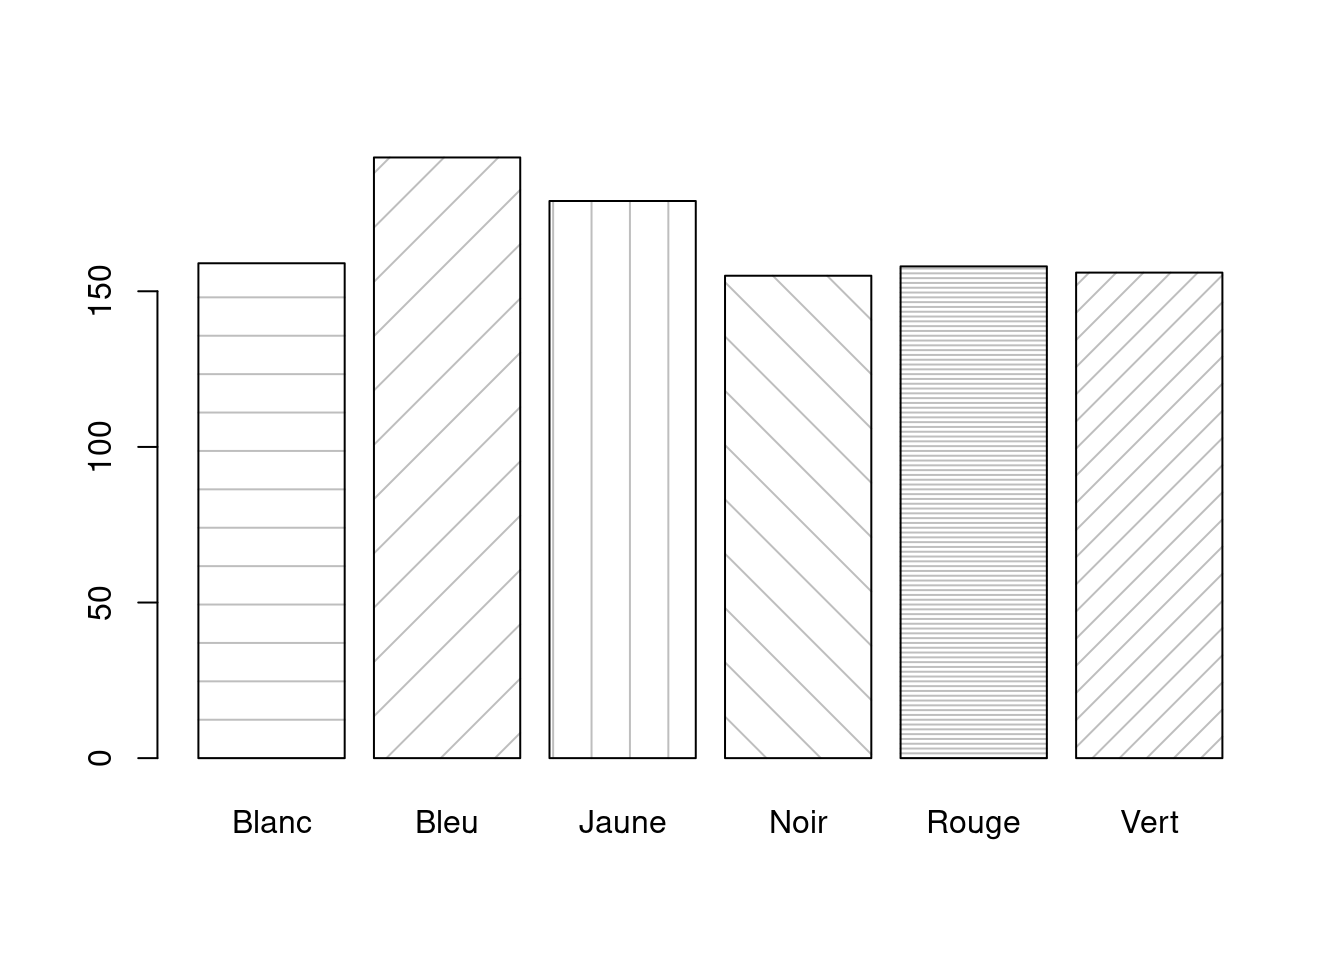
\includegraphics[width=0.6\linewidth]{visualiseR_files/figure-latex/unnamed-chunk-54-1} \end{center}

\hypertarget{histogramme}{%
\subsection{Histogramme}\label{histogramme}}

L'histogramme permet de visualiser la répartition des valeurs d'une variable continue en créant des classes de valeurs. Il est très utile pour connaître la loi
de distribution que suivent les valeurs (loi normale, loi de Poisson, etc.). Sous R, ce graphe se fera à l'aide de la fonction \texttt{hist()}.
Générons 1000 valeurs aléatoires selon une loi gaussienne.

\begin{Shaded}
\begin{Highlighting}[]
\NormalTok{var6 <-}\StringTok{ }\KeywordTok{rnorm}\NormalTok{(}\DataTypeTok{n =} \DecValTok{1000}\NormalTok{)}
\NormalTok{var6[}\DecValTok{1}\OperatorTok{:}\DecValTok{20}\NormalTok{]}
\CommentTok{#>  [1] -0.90998297 -0.71083254  0.83173313  0.39938518  0.67614094  1.19805087}
\CommentTok{#>  [7] -0.25563620 -0.15618080 -2.67672559 -1.13728008 -0.29537803  0.95859818}
\CommentTok{#> [13] -1.81219676  0.09119575  0.89121128  2.28531255  0.17138918  0.15748998}
\CommentTok{#> [19]  2.13348921  0.20186680}
\end{Highlighting}
\end{Shaded}

\begin{Shaded}
\begin{Highlighting}[]
\KeywordTok{hist}\NormalTok{(var6)}
\end{Highlighting}
\end{Shaded}

\begin{center}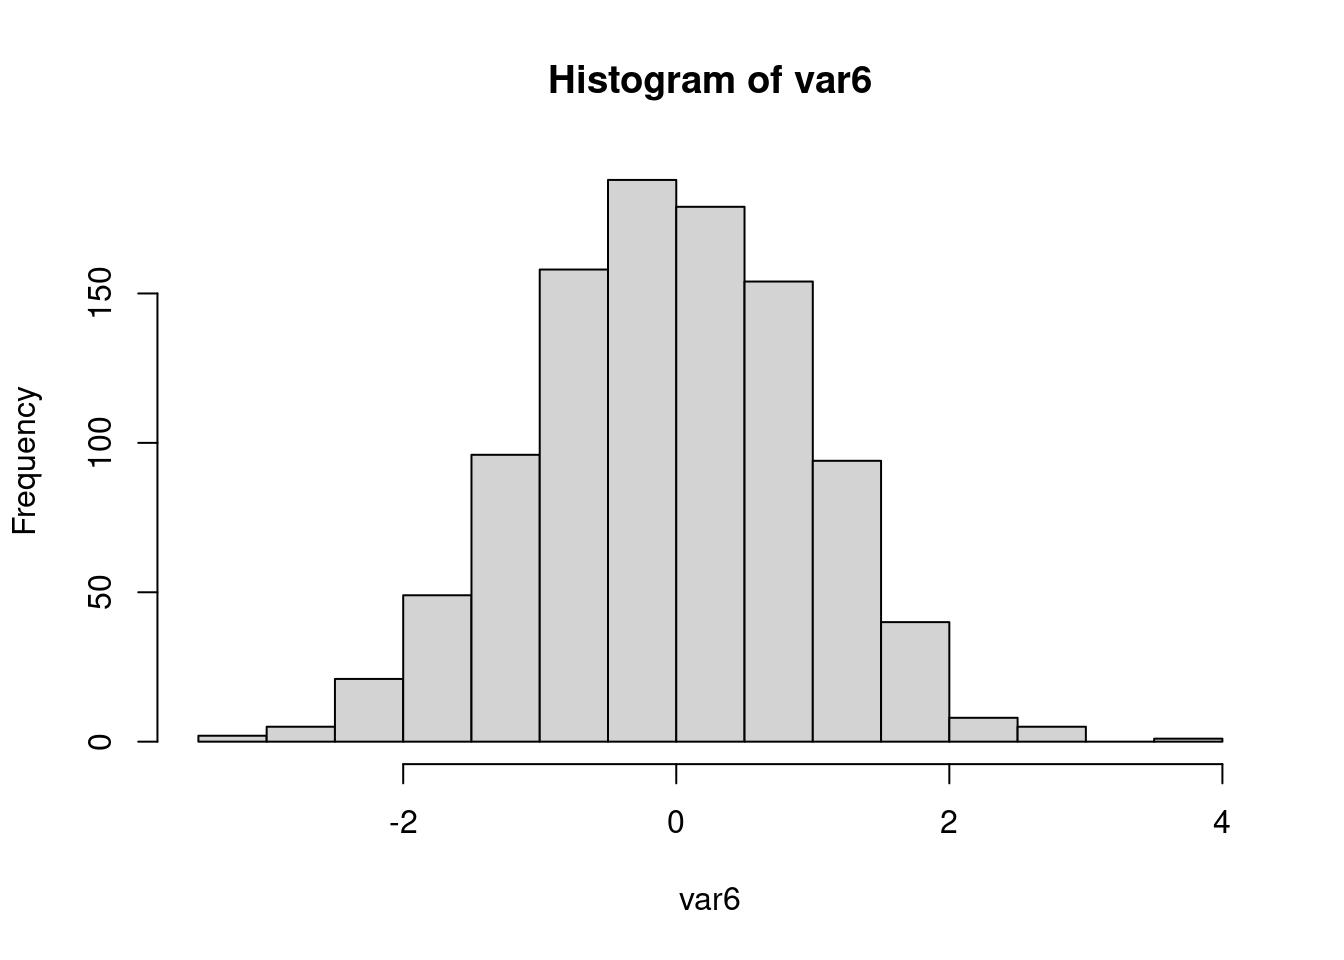
\includegraphics{visualiseR_files/figure-latex/unnamed-chunk-56-1} \end{center}

De la même manière que pour les boîtes à moustaches, l'argument \texttt{plot\ =\ FALSE} ne trace pas l'histogramme, mais affiche dans la console les statistiques associées.

\begin{Shaded}
\begin{Highlighting}[]
\KeywordTok{hist}\NormalTok{(var6, }\DataTypeTok{plot =} \OtherTok{FALSE}\NormalTok{)}
\CommentTok{#> $breaks}
\CommentTok{#>  [1] -3.5 -3.0 -2.5 -2.0 -1.5 -1.0 -0.5  0.0  0.5  1.0  1.5  2.0  2.5  3.0}
\CommentTok{#> }
\CommentTok{#> $counts}
\CommentTok{#>  [1]   1   4  16  37  96 173 190 179 150  97  36  17   4}
\CommentTok{#> }
\CommentTok{#> $density}
\CommentTok{#>  [1] 0.002 0.008 0.032 0.074 0.192 0.346 0.380 0.358 0.300 0.194 0.072 0.034}
\CommentTok{#> [13] 0.008}
\CommentTok{#> }
\CommentTok{#> $mids}
\CommentTok{#>  [1] -3.25 -2.75 -2.25 -1.75 -1.25 -0.75 -0.25  0.25  0.75  1.25  1.75  2.25}
\CommentTok{#> [13]  2.75}
\CommentTok{#> }
\CommentTok{#> $xname}
\CommentTok{#> [1] "var6"}
\CommentTok{#> }
\CommentTok{#> $equidist}
\CommentTok{#> [1] TRUE}
\CommentTok{#> }
\CommentTok{#> attr(,"class")}
\CommentTok{#> [1] "histogram"}
\end{Highlighting}
\end{Shaded}

L'argument \texttt{breaks} permet de modifier les classes de l'histogramme. Une façon
simple de procéder consiste à donner le nombre de classes que l'on souhaite
représenter.

\begin{Shaded}
\begin{Highlighting}[]
\KeywordTok{hist}\NormalTok{(var6, }\DataTypeTok{breaks =} \DecValTok{30}\NormalTok{)}
\end{Highlighting}
\end{Shaded}

\begin{center}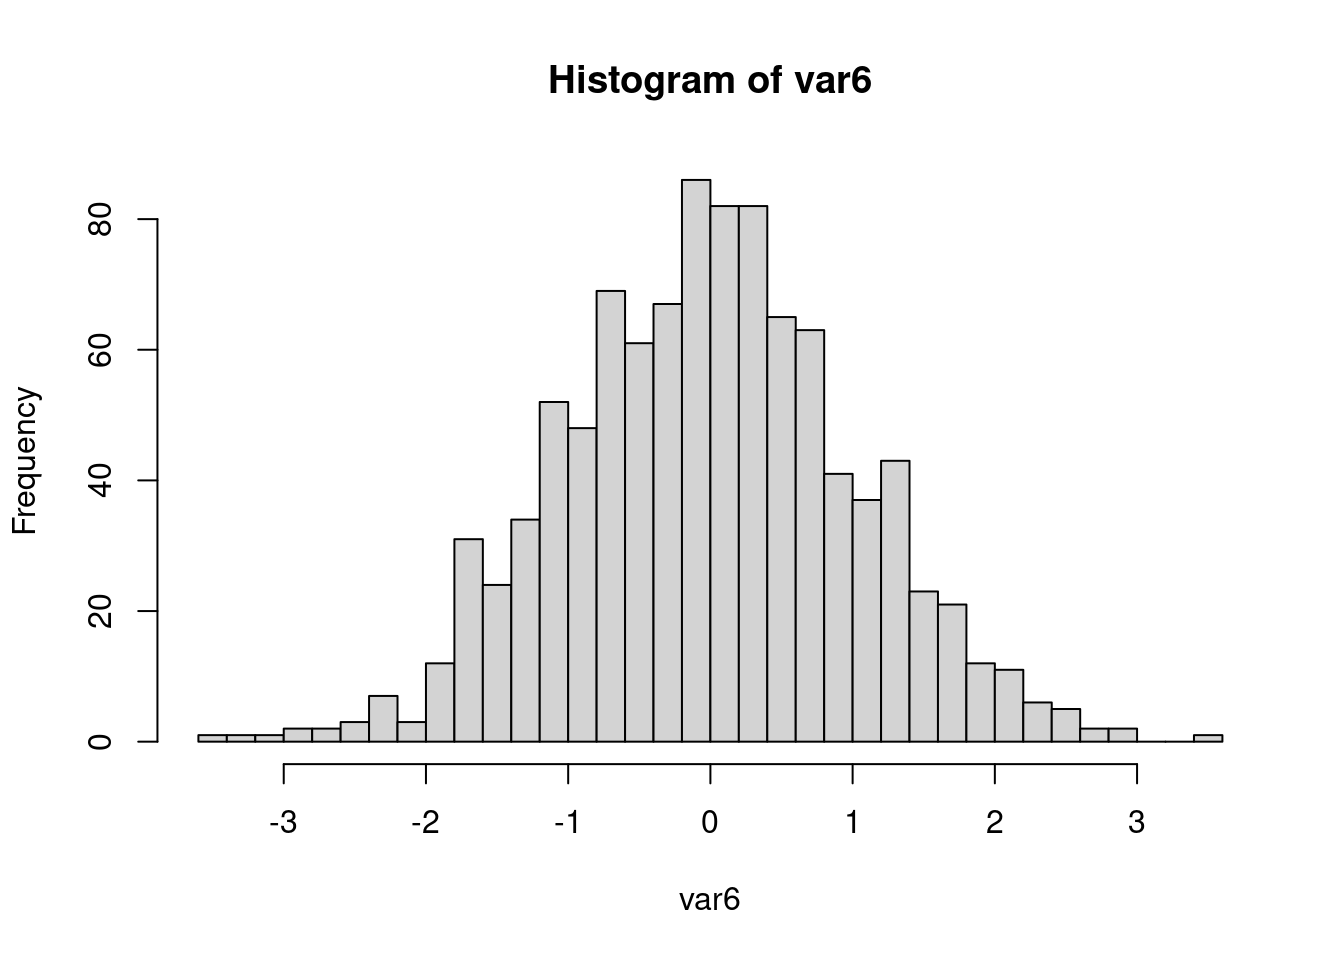
\includegraphics[width=0.6\linewidth]{visualiseR_files/figure-latex/unnamed-chunk-58-1} \end{center}

Nous aurions également pu indiquer les bornes de chaque classe désirée (par ex.
des classes tous les 0.25). De même, plusieurs algorithmes ont été implémentés
afin de déterminer un nombre de classes \texttt{optimum} . Consultez l'aide de cette
fonction pour en savoir plus.

\begin{Shaded}
\begin{Highlighting}[]
\KeywordTok{help}\NormalTok{(hist)}
\end{Highlighting}
\end{Shaded}

Finalement, mentionnons que les arguments \texttt{density} et \texttt{angle} sont aussi disponibles pour la fonction \texttt{hist()}. Adéquatement définis, ils permettront d'hachurer les rectangles.

\hypertarget{diagramme-sectoriel}{%
\subsection{Diagramme sectoriel}\label{diagramme-sectoriel}}

Une alternative au diagramme en bâtons est le diagramme sectoriel (camembert). Regardons ce que ça donne avec les données précédentes (couleurs).

\begin{Shaded}
\begin{Highlighting}[]
\KeywordTok{pie}\NormalTok{(var4, }\DataTypeTok{col =} \KeywordTok{c}\NormalTok{(}\StringTok{"white"}\NormalTok{, }\StringTok{"blue"}\NormalTok{, }\StringTok{"yellow"}\NormalTok{, }\StringTok{"black"}\NormalTok{, }\StringTok{"red"}\NormalTok{, }\StringTok{"green"}\NormalTok{))}
\end{Highlighting}
\end{Shaded}

\begin{center}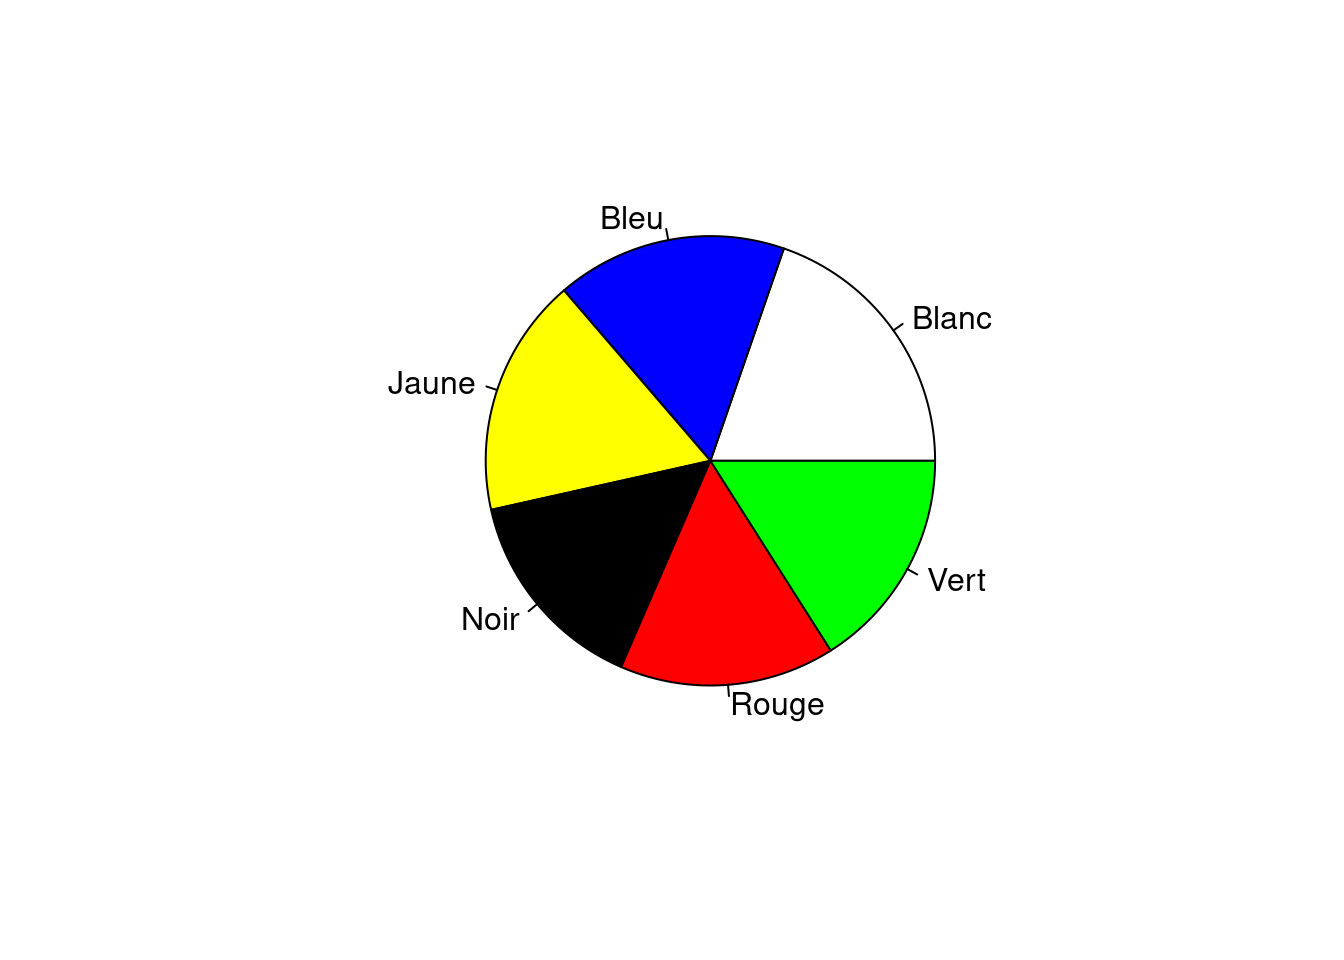
\includegraphics[width=0.6\linewidth]{visualiseR_files/figure-latex/unnamed-chunk-60-1} \end{center}

\begin{Shaded}
\begin{Highlighting}[]
\KeywordTok{pie}\NormalTok{(}\KeywordTok{rep}\NormalTok{(}\DecValTok{1}\NormalTok{, }\DecValTok{250}\NormalTok{), }\DataTypeTok{col =} \KeywordTok{rainbow}\NormalTok{(}\DecValTok{250}\NormalTok{), }\DataTypeTok{border =} \OtherTok{NA}\NormalTok{, }\DataTypeTok{labels =} \StringTok{""}\NormalTok{)}
\end{Highlighting}
\end{Shaded}

\begin{center}
\includegraphics[width=0.6\linewidth]{visualiseR_files/figure-latex/unnamed-chunk-61-1} \end{center}

Dans les deux exemples précédents, nous avons défini des couleurs à l'aide de l'argument \texttt{col}. Dans le premier cas, nous avons indiqué le nom des couleurs : R implémente une palette de couleurs prédéfinies assez conséquente. Dans le second cas, nous avons utilisé la fonction \texttt{rainbow()} qui sélectionne un nombre donné de couleurs parmi les couleurs de l'arc-en-ciel. Nous y reviendrons dans le troisième chapitre.

Pour terminer, exécutez le code suivant sous R.

\begin{Shaded}
\begin{Highlighting}[]
\ControlFlowTok{for}\NormalTok{ (i }\ControlFlowTok{in} \DecValTok{1} \OperatorTok{:}\StringTok{ }\DecValTok{250}\NormalTok{)\{}
  \ControlFlowTok{if}\NormalTok{ (i }\OperatorTok{>}\StringTok{ }\DecValTok{1}\NormalTok{)\{}
\NormalTok{    cols <-}\StringTok{ }\KeywordTok{rainbow}\NormalTok{(}\DecValTok{250}\NormalTok{)[}\KeywordTok{c}\NormalTok{(i}\OperatorTok{:}\DecValTok{250}\NormalTok{, }\DecValTok{1}\OperatorTok{:}\NormalTok{(i}\DecValTok{-1}\NormalTok{))]}
    \KeywordTok{pie}\NormalTok{(}\KeywordTok{rep}\NormalTok{(}\DecValTok{1}\NormalTok{, }\DecValTok{250}\NormalTok{), }\DataTypeTok{col =}\NormalTok{ cols, }\DataTypeTok{border =} \OtherTok{NA}\NormalTok{, }\DataTypeTok{labels =} \StringTok{""}\NormalTok{)}
\NormalTok{  \}}\ControlFlowTok{else}\NormalTok{\{}
    \KeywordTok{pie}\NormalTok{(}\KeywordTok{rep}\NormalTok{(}\DecValTok{1}\NormalTok{, }\DecValTok{250}\NormalTok{), }\DataTypeTok{col =} \KeywordTok{rainbow}\NormalTok{(}\DecValTok{250}\NormalTok{), }\DataTypeTok{border =} \OtherTok{NA}\NormalTok{, }\DataTypeTok{labels =} \StringTok{""}\NormalTok{)}
\NormalTok{  \}}
\NormalTok{\}}
\end{Highlighting}
\end{Shaded}

Plutôt sympa, non ?

\hypertarget{fonctions-mathuxe9matiques}{%
\subsection{Fonctions mathématiques}\label{fonctions-mathuxe9matiques}}

Pour terminer ce chapitre, introduisons une fonction qui pourrait vous être utile. Il s'agit de la fonction \texttt{curve()} qui permet de tracer le comportement d'une fonction mathématique bornée. Regardons un exemple avec des fonctions trigonométriques.

\begin{Shaded}
\begin{Highlighting}[]
\KeywordTok{par}\NormalTok{(}\DataTypeTok{mfrow =} \KeywordTok{c}\NormalTok{(}\DecValTok{1}\NormalTok{, }\DecValTok{3}\NormalTok{), }\DataTypeTok{mgp =} \KeywordTok{c}\NormalTok{(}\DecValTok{2}\NormalTok{, }\DecValTok{1}\NormalTok{, }\DecValTok{0}\NormalTok{))}
\NormalTok{txt <-}\StringTok{ }\KeywordTok{expression}\NormalTok{(}\KeywordTok{f}\NormalTok{(x)}\OperatorTok{==}\KeywordTok{cos}\NormalTok{(x))}
\KeywordTok{curve}\NormalTok{(}\KeywordTok{cos}\NormalTok{(x), }\DataTypeTok{from =} \DecValTok{-10}\NormalTok{, }\DataTypeTok{to =} \DecValTok{10}\NormalTok{, }\DataTypeTok{main =} \StringTok{"Cosinus"}\NormalTok{, }\DataTypeTok{ylab =}\NormalTok{ txt)}
\NormalTok{txt <-}\StringTok{ }\KeywordTok{expression}\NormalTok{(}\KeywordTok{f}\NormalTok{(x)}\OperatorTok{==}\KeywordTok{sin}\NormalTok{(x))}
\KeywordTok{curve}\NormalTok{(}\KeywordTok{sin}\NormalTok{(x), }\DataTypeTok{from =} \DecValTok{-10}\NormalTok{, }\DataTypeTok{to =} \DecValTok{10}\NormalTok{, }\DataTypeTok{main =} \StringTok{"Sinus"}\NormalTok{, }\DataTypeTok{ylab =}\NormalTok{ txt)}
\NormalTok{txt <-}\StringTok{ }\KeywordTok{expression}\NormalTok{(}\KeywordTok{f}\NormalTok{(x)}\OperatorTok{==}\KeywordTok{tan}\NormalTok{(x))}
\KeywordTok{curve}\NormalTok{(}\KeywordTok{tan}\NormalTok{(x), }\DataTypeTok{from =} \DecValTok{-10}\NormalTok{, }\DataTypeTok{to =} \DecValTok{10}\NormalTok{, }\DataTypeTok{main =} \StringTok{"Tangente"}\NormalTok{, }\DataTypeTok{ylab =}\NormalTok{ txt)}
\end{Highlighting}
\end{Shaded}

\begin{center}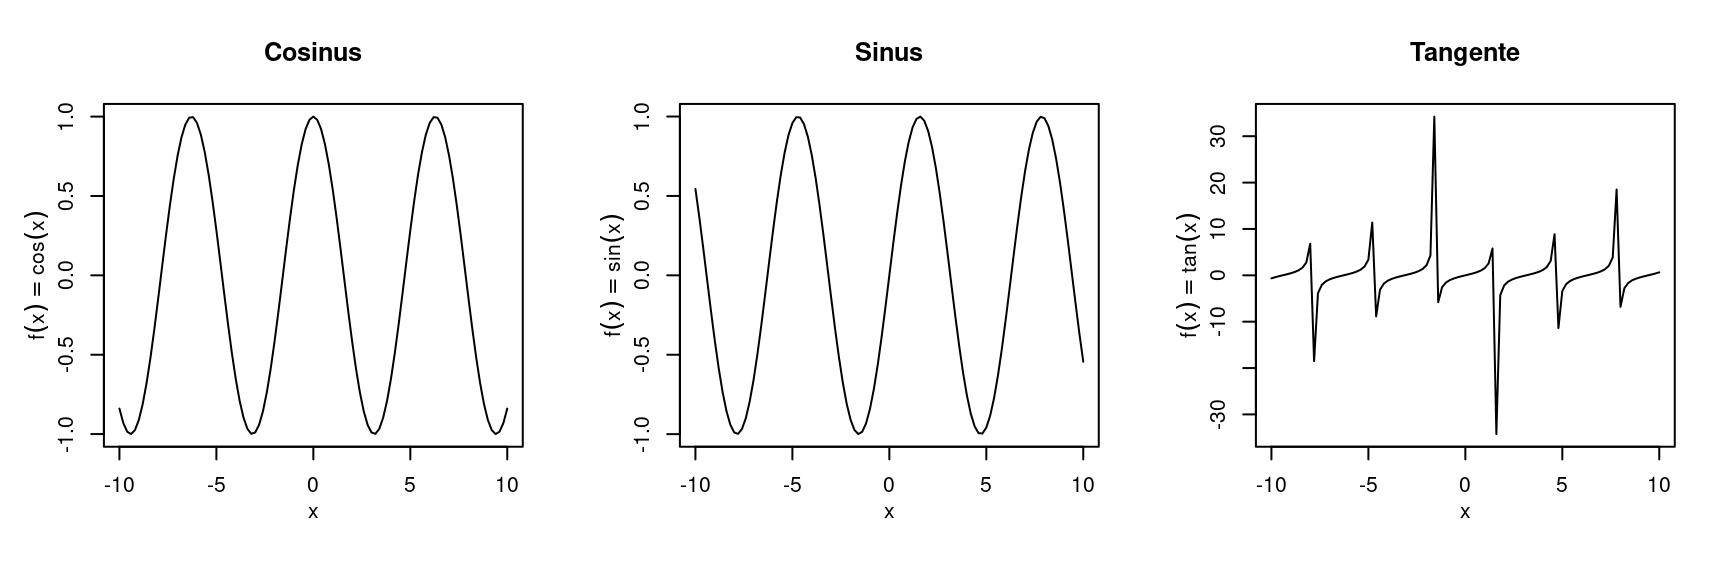
\includegraphics[width=1\linewidth]{visualiseR_files/figure-latex/unnamed-chunk-63-1} \end{center}

Ici, des éclaircissements s'imposent. Premièrement, nous avons modifié un autre paramètre graphique : \texttt{mgp}. Celui permet de contrôler le positionnement du nom des axes, des étiquettes des axes et des axes eux-mêmes. Ces positionnements sont relatifs à la région du plot. Nous y reviendrons plus loin.
La fonction \texttt{expression()} permet quant à elle d'utiliser l'écriture mathématique dans des graphiques. Consultez l'aide de cette fonction ainsi que celle de la fonction \texttt{plotmath()} pour en savoir plus.

\begin{Shaded}
\begin{Highlighting}[]
\KeywordTok{par}\NormalTok{(}\DataTypeTok{mfrow =} \KeywordTok{c}\NormalTok{(}\DecValTok{2}\NormalTok{, }\DecValTok{3}\NormalTok{), }\DataTypeTok{mgp =} \KeywordTok{c}\NormalTok{(}\DecValTok{2}\NormalTok{, }\DecValTok{1}\NormalTok{, }\DecValTok{0}\NormalTok{))}
\NormalTok{txt <-}\StringTok{ }\KeywordTok{expression}\NormalTok{(}\KeywordTok{f}\NormalTok{(x)}\OperatorTok{==}\NormalTok{x)}
\KeywordTok{curve}\NormalTok{(x}\OperatorTok{^}\DecValTok{1}\NormalTok{, }\DataTypeTok{from =} \DecValTok{-1}\NormalTok{, }\DataTypeTok{to =} \DecValTok{1}\NormalTok{, }\DataTypeTok{main =} \StringTok{"Identité"}\NormalTok{, }\DataTypeTok{ylab =}\NormalTok{ txt)}
\NormalTok{txt <-}\StringTok{ }\KeywordTok{expression}\NormalTok{(}\KeywordTok{f}\NormalTok{(x)}\OperatorTok{==}\NormalTok{x}\OperatorTok{^}\DecValTok{2}\NormalTok{)}
\KeywordTok{curve}\NormalTok{(x}\OperatorTok{^}\DecValTok{2}\NormalTok{, }\DataTypeTok{from =} \DecValTok{-1}\NormalTok{, }\DataTypeTok{to =} \DecValTok{1}\NormalTok{, }\DataTypeTok{main =} \StringTok{"Quadratique"}\NormalTok{, }\DataTypeTok{ylab =}\NormalTok{ txt)}
\NormalTok{txt <-}\StringTok{ }\KeywordTok{expression}\NormalTok{(}\KeywordTok{f}\NormalTok{(x)}\OperatorTok{==}\NormalTok{x}\OperatorTok{^}\DecValTok{3}\NormalTok{)}
\KeywordTok{curve}\NormalTok{(x}\OperatorTok{^}\DecValTok{3}\NormalTok{, }\DataTypeTok{from =} \DecValTok{-1}\NormalTok{, }\DataTypeTok{to =} \DecValTok{1}\NormalTok{, }\DataTypeTok{main =} \StringTok{"Cubique"}\NormalTok{, }\DataTypeTok{ylab =}\NormalTok{ txt)}
\NormalTok{txt <-}\StringTok{ }\KeywordTok{expression}\NormalTok{(}\KeywordTok{f}\NormalTok{(x)}\OperatorTok{==}\DecValTok{1}\OperatorTok{/}\NormalTok{x)}
\KeywordTok{curve}\NormalTok{(}\DecValTok{1}\OperatorTok{/}\NormalTok{x, }\DataTypeTok{from =} \DecValTok{-1}\NormalTok{, }\DataTypeTok{to =} \DecValTok{1}\NormalTok{, }\DataTypeTok{main =} \StringTok{"Inverse"}\NormalTok{, }\DataTypeTok{ylab =}\NormalTok{ txt)}
\NormalTok{txt <-}\StringTok{ }\KeywordTok{expression}\NormalTok{(}\KeywordTok{f}\NormalTok{(x)}\OperatorTok{==}\KeywordTok{log}\NormalTok{(x))}
\KeywordTok{curve}\NormalTok{(}\KeywordTok{log}\NormalTok{(x), }\DataTypeTok{from =} \FloatTok{0.0001}\NormalTok{, }\DataTypeTok{to =} \DecValTok{10}\NormalTok{, }\DataTypeTok{main =} \StringTok{"Logarithme"}\NormalTok{, }\DataTypeTok{ylab =}\NormalTok{ txt)}
\NormalTok{txt <-}\StringTok{ }\KeywordTok{expression}\NormalTok{(}\KeywordTok{f}\NormalTok{(x)}\OperatorTok{==}\KeywordTok{exp}\NormalTok{(x))}
\KeywordTok{curve}\NormalTok{(}\KeywordTok{exp}\NormalTok{(x), }\DataTypeTok{from =} \FloatTok{0.0001}\NormalTok{, }\DataTypeTok{to =} \DecValTok{10}\NormalTok{, }\DataTypeTok{main =} \StringTok{"Exponentielle"}\NormalTok{, }\DataTypeTok{ylab =}\NormalTok{ txt)}
\end{Highlighting}
\end{Shaded}

\begin{center}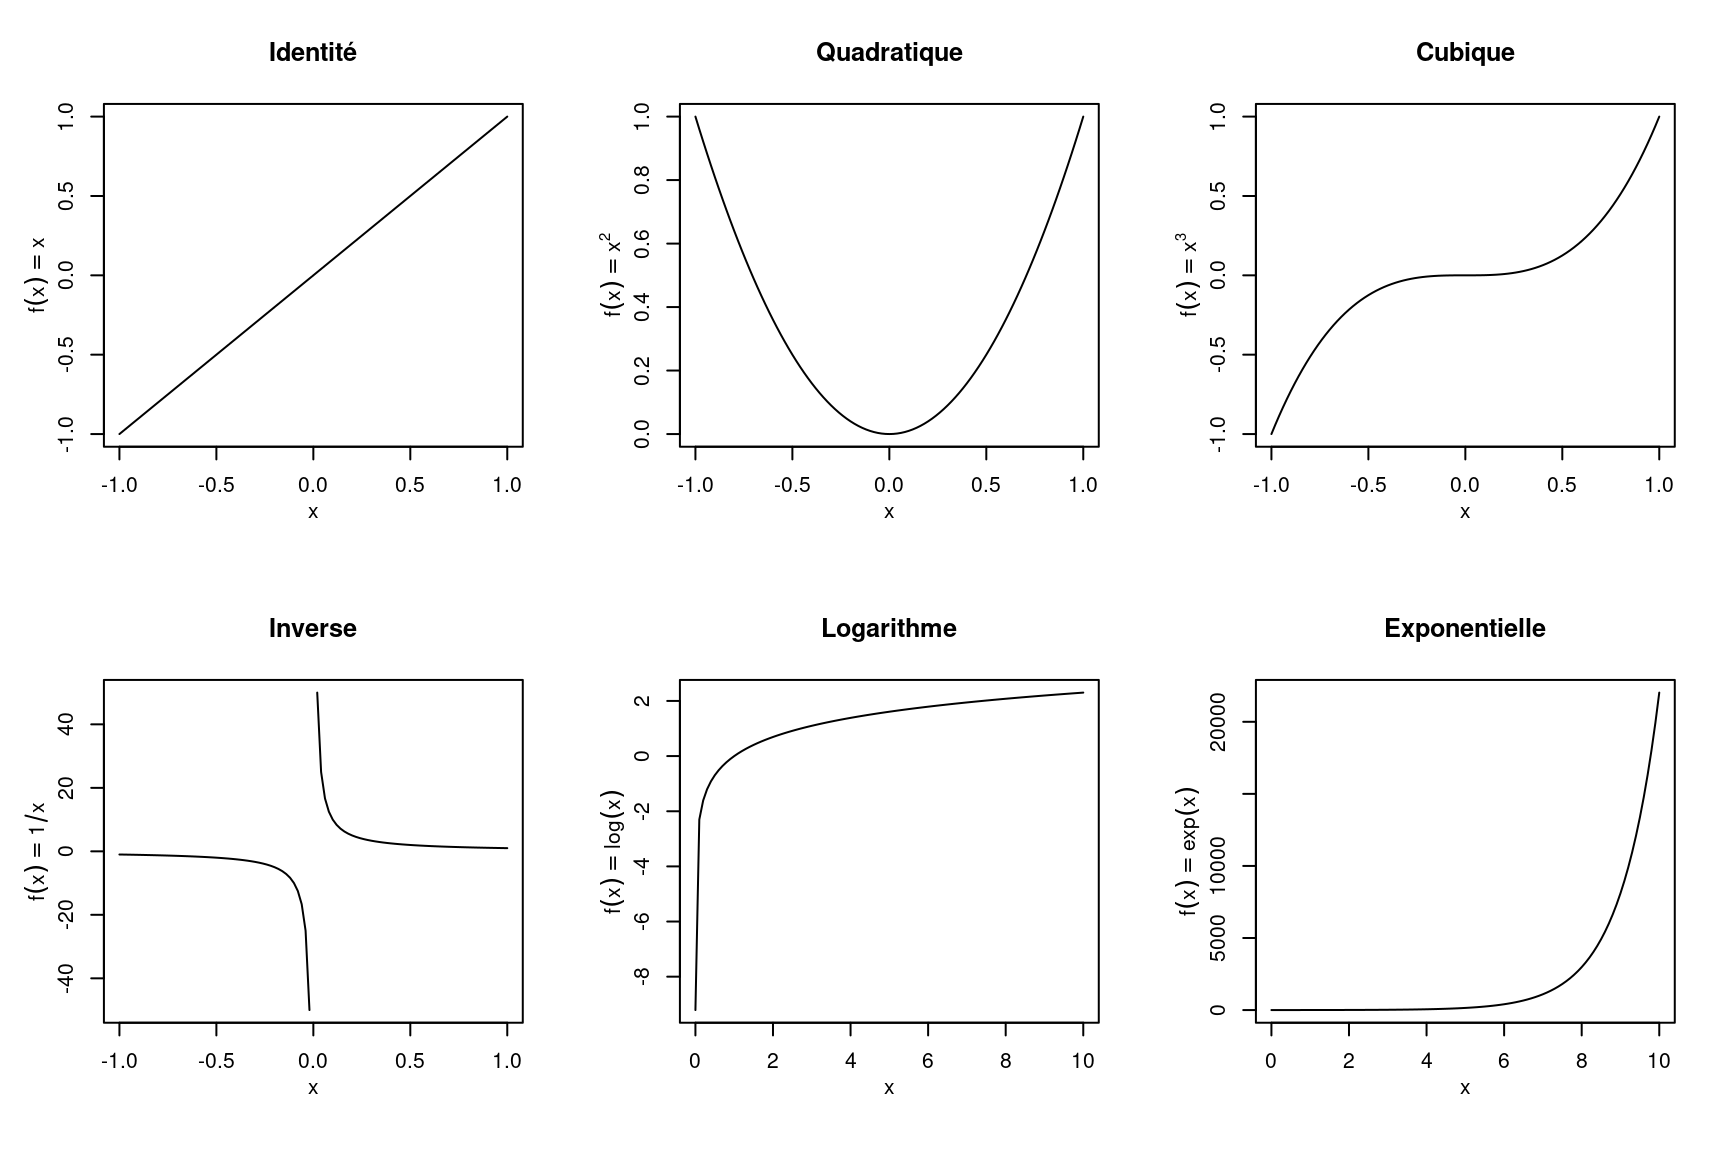
\includegraphics[width=1\linewidth]{visualiseR_files/figure-latex/unnamed-chunk-64-1} \end{center}

\hypertarget{paramuxe8tres-graphiques}{%
\section{Paramètres graphiques}\label{paramuxe8tres-graphiques}}

Au cours des deux derniers chapitres, nous avons vu comment créer et éditer un graphe à l'aide des principales fonctions contenues dans le package \texttt{graphics}. Dans ce troisième chapitre, nous allons approfondir les notions introduites précédemment, notamment en ce qui a trait aux paramètres graphiques principaux, tels que les fontes de caractères, les types de symboles et de lignes, les axes, les marges, etc. Nous terminerons ce chapitre en nous attardant sur les couleurs sous R, et plus généralement, dans le monde informatique. En effet, ce que nous dirons sur les fontes de caractères et les couleurs sera aussi valable dans le développement Web (e.g.~CSS pour \emph{Cascading Style Sheets}, ou feuilles de style en français).

\hypertarget{la-fonction-par}{%
\subsection{\texorpdfstring{La fonction \texttt{par()}}{La fonction par()}}\label{la-fonction-par}}

Précédemment, nous avons mentionné que lorsque R trace ou édite un graphe, il va récupérer les valeurs des paramètres graphiques pour adapter les axes, le background, les couleurs, les tailles de caractères, etc. Celles-ci sont stockées dans l'objet \texttt{par()}, qui est également une fonction. En effet, l'affichage d'un paramètre se fait en appelant l'objet (le paramètre est un élément de la liste \texttt{par()}), mais le changement de valeur d'un paramètre se fait en appelant la fonction (le paramètre devient un argument de la fonction \texttt{par()}).

\begin{Shaded}
\begin{Highlighting}[]
\KeywordTok{par}\NormalTok{()}\OperatorTok{$}\NormalTok{bg}
\CommentTok{#> [1] "white"}
\KeywordTok{par}\NormalTok{()}\OperatorTok{$}\NormalTok{col}
\CommentTok{#> [1] "black"}
\KeywordTok{par}\NormalTok{()}\OperatorTok{$}\NormalTok{bty}
\CommentTok{#> [1] "o"}
\end{Highlighting}
\end{Shaded}

Ces paramètres possèdent des valeurs par défaut afin d'éviter à l'utilisateur de devoir les définir à chaque nouveau graphe. Bien entendu, ces valeurs peuvent être modifiées : heureusement, car même si les valeurs par défaut conviennent à n'importe quelle représentation graphique, le rendu visuel laisse vraiment à désirer. Nous avons déjà modifié les valeurs par défaut de certains paramètres (axes, couleurs, etc.), soit directement dans les fonctions appelées (e.g. \texttt{plot()}, \texttt{axis()}, \texttt{legend()}, \texttt{polygon()}, etc.), soit dans la fonction \texttt{par()}.
Et, c'est là une notion très importante : les paramètres graphiques peuvent être modifiés soit dans le \texttt{par()}, soit à la volée, dans les fonctions graphiques. Mentionnons tout de même que certains paramètres ne peuvent être modifiés que via la fonction \texttt{par()}. C'est le cas notamment de \texttt{mar}, \texttt{oma}, \texttt{new}, \texttt{fig}, \texttt{mfcol} et \texttt{mfrow}.

Mais, la modification dans le \texttt{par()} n'aura pas le même effet qu'une modification à la volée. En effet, modifier la couleur du texte dans la fonction \texttt{plot()} n'aura pas pour conséquence de mettre à jour la valeur de cet argument dans le \texttt{par()}. Ainsi, si derrière nous rajoutons, par ex. un titre avec la fonction \texttt{title()} sans spécifier de couleur, celui-ci s'affichera avec la valeur par défaut contenue dans le \texttt{par()}. Au contraire, si on modifie la couleur du texte dans le \texttt{par()}, et qu'aucune précision n'est apportée à la volée concernant ce paramètre, toutes les fonctions graphiques afficheront la couleur du texte selon la nouvelle valeur définie dans le \texttt{par()}.
Un dernier point important : toute modification dans la fonction \texttt{par()} sera effective tant qu'un périphérique graphique restera ouvert. La fermeture des périphériques graphiques entraînera la remise à zéro des valeurs des paramètres graphiques. Cependant, il est de coutume de sauvegarder les paramètres graphiques avec leurs valeurs par défaut dans un objet, et de redéfinir le \texttt{par()} avec cet objet une fois le graphique réalisé. Ceci permet de s'assurer que le \texttt{par()} est bien réinitialisé.

\begin{Shaded}
\begin{Highlighting}[]
\CommentTok{## Sauvegarde du par() d'origine}
\NormalTok{opar <-}\StringTok{ }\KeywordTok{par}\NormalTok{()}
\CommentTok{## Modification du par()}
\KeywordTok{par}\NormalTok{(}\DataTypeTok{bg =} \StringTok{"steelblue"}\NormalTok{, }\DataTypeTok{mar =} \KeywordTok{c}\NormalTok{(}\DecValTok{1}\NormalTok{, }\DecValTok{1}\NormalTok{, }\DecValTok{0}\NormalTok{, }\DecValTok{0}\NormalTok{), }\DataTypeTok{col =} \StringTok{"white"}\NormalTok{)}
\CommentTok{## Commandes graphiques...}
\CommentTok{## Restauration du par()}
\KeywordTok{par}\NormalTok{(opar)}
\end{Highlighting}
\end{Shaded}

La fonction \texttt{par()} comporte 72 paramètres graphiques dont la plupart sont modifiables (66 pour être précis). Au cours de ce chapitre, nous allons en détailler une bonne trentaine, ceux que nous avons jugés les plus pertinents.

\hypertarget{fonte-de-caractuxe8res}{%
\subsection{Fonte de caractères}\label{fonte-de-caractuxe8res}}

Abordons tout d'abord la notion de fonte de caractères. En typographie, une fonte de caractères est un ensemble de règles qui va déterminer le rendu visuel d'une expression textuelle. Il est très fréquent que police et fonte soient confondues. Une fonte de caractère est caractérisée par :
- une police de caractères (\emph{font family} ou \emph{typeface} en anglais);
- un style (normal, italique ou oblique);
- une graisse (normal ou gras);
- un corps (taille de police).

Ainsi, le Helvetica normal 12 points est une fonte de caractères, mais le
Helvetica est une police de caractères. De nombreuses classifications existent
pour les polices de caractères. Celle que nous présentons ici à l'avantage de se
rapprocher des polices disponibles dans R (et dans le monde du Web). Sous R,
trois polices principales de caractères sont disponibles :

\begin{itemize}
\tightlist
\item
  sans-serif (noté \texttt{sans}) : regroupe les polices sans empattement (c.-à-d. sans les extensions qui viennent terminer les caractères) et à chasse proportionnelle (la largeur des caractères varie en fonction du caractère). Citons le Helvetica, Arial et Verdana comme police sans-serif.
\item
  serif (noté \texttt{serif}) : regroupe les polices à empattement et à chasse proportionnelle. C'est le cas du Times (New Roman) et du Garamond.
\item
  monospace (noté \texttt{mono}) : possède la caractéristique d'avoir une chasse fixe. Ses polices sont préférées pour l'écriture de code informatique car elles permettent un alignement vertical des caractères. R, sous Windows, utilise la police Courier New et sous Mac, le Monaco.
  Par défaut, la police \texttt{sans} est utilisée sous R pour afficher l'information textuelle sur les graphes. Cette valeur est stockée dans l'argument \texttt{family} du \texttt{par()}. Regardons les différences entre ces trois polices de caractères.
\end{itemize}

\begin{Shaded}
\begin{Highlighting}[]
\KeywordTok{par}\NormalTok{(}\DataTypeTok{mfrow =} \KeywordTok{c}\NormalTok{(}\DecValTok{2}\NormalTok{, }\DecValTok{2}\NormalTok{), }\DataTypeTok{bg =} \StringTok{"lightgray"}\NormalTok{)}
\KeywordTok{plot}\NormalTok{(}\DecValTok{0}\NormalTok{, }\DataTypeTok{type =} \StringTok{"n"}\NormalTok{)}
\KeywordTok{text}\NormalTok{(}\DecValTok{1}\NormalTok{, }\DecValTok{0}\NormalTok{, }\StringTok{"Police par défaut"}\NormalTok{, }\DataTypeTok{cex =} \DecValTok{2}\NormalTok{)}
\KeywordTok{plot}\NormalTok{(}\DecValTok{0}\NormalTok{, }\DataTypeTok{type =} \StringTok{"n"}\NormalTok{, }\DataTypeTok{family =} \StringTok{"sans"}\NormalTok{)}
\KeywordTok{text}\NormalTok{(}\DecValTok{1}\NormalTok{, }\DecValTok{0}\NormalTok{, }\DataTypeTok{family =} \StringTok{"sans"}\NormalTok{, }\StringTok{"Police sans serif"}\NormalTok{, }\DataTypeTok{cex =} \DecValTok{2}\NormalTok{)}
\KeywordTok{plot}\NormalTok{(}\DecValTok{0}\NormalTok{, }\DataTypeTok{type =} \StringTok{"n"}\NormalTok{, }\DataTypeTok{family =} \StringTok{"serif"}\NormalTok{)}
\KeywordTok{text}\NormalTok{(}\DecValTok{1}\NormalTok{, }\DecValTok{0}\NormalTok{, }\DataTypeTok{family =} \StringTok{"serif"}\NormalTok{, }\StringTok{"Police serif"}\NormalTok{, }\DataTypeTok{cex =} \DecValTok{2}\NormalTok{)}
\KeywordTok{plot}\NormalTok{(}\DecValTok{0}\NormalTok{, }\DataTypeTok{type =} \StringTok{"n"}\NormalTok{, }\DataTypeTok{family =} \StringTok{"mono"}\NormalTok{)}
\KeywordTok{text}\NormalTok{(}\DecValTok{1}\NormalTok{, }\DecValTok{0}\NormalTok{, }\DataTypeTok{family =} \StringTok{"mono"}\NormalTok{, }\StringTok{"Police mono"}\NormalTok{, }\DataTypeTok{cex =} \DecValTok{2}\NormalTok{)}
\end{Highlighting}
\end{Shaded}

\begin{center}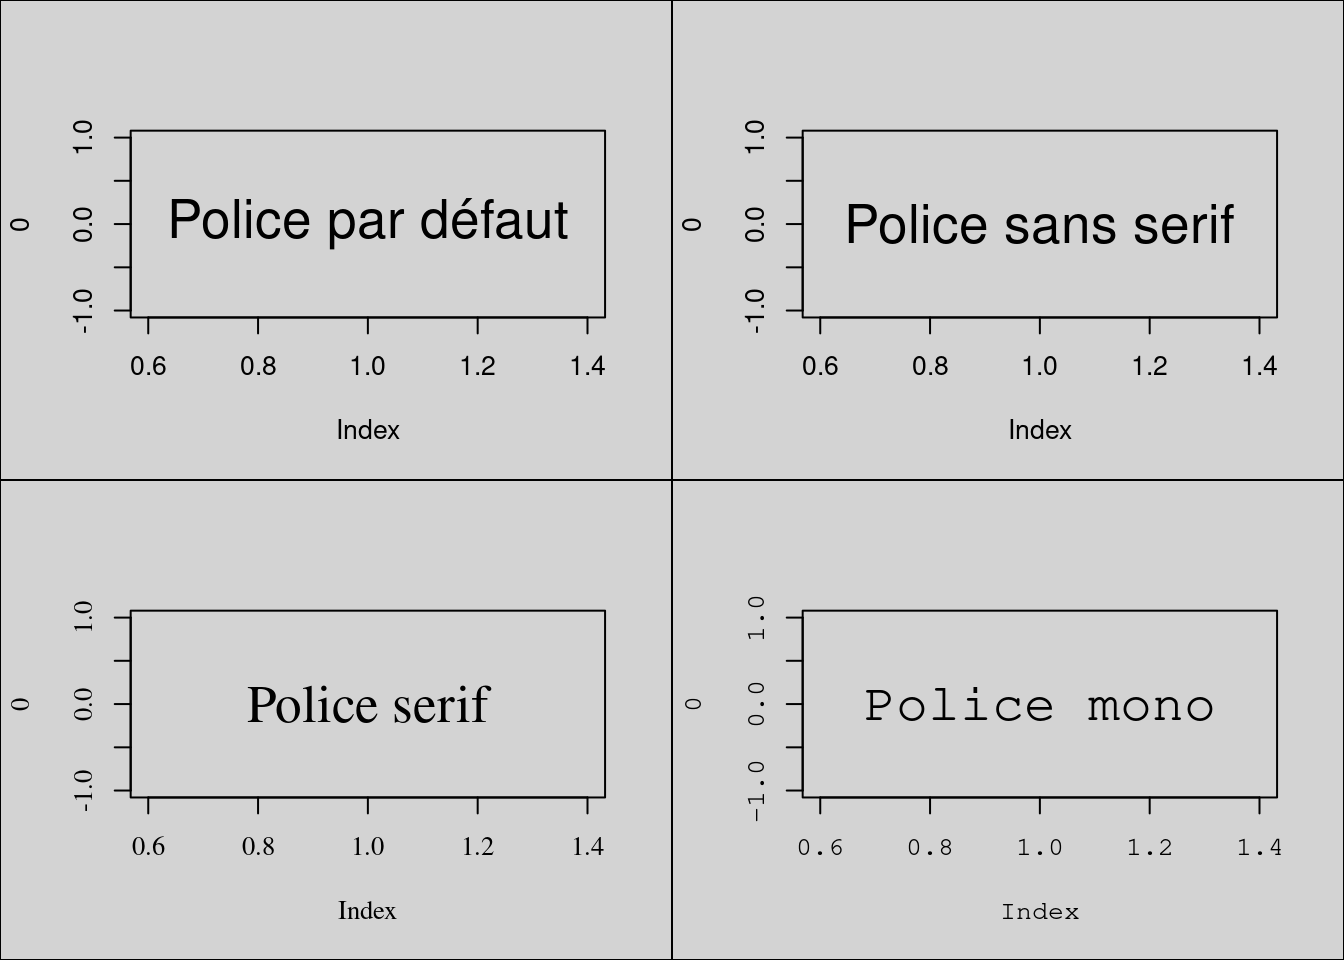
\includegraphics[width=0.6\linewidth]{visualiseR_files/figure-latex/unnamed-chunk-67-1} \end{center}

Sous R, le style et la graisse sont regroupés sous le même argument : \texttt{font}. Mais, celui-ci est plus précis que \texttt{family} (qui s'applique sur tous les éléments textuels) dans le sens où il se décline en \texttt{font.axis}, \texttt{font.lab}, \texttt{font.main} et \texttt{font.sub}. Regardons les différents styles disponibles.

\begin{Shaded}
\begin{Highlighting}[]
\KeywordTok{par}\NormalTok{(}\DataTypeTok{mfrow =} \KeywordTok{c}\NormalTok{(}\DecValTok{2}\NormalTok{, }\DecValTok{2}\NormalTok{), }\DataTypeTok{bg =} \StringTok{"lightgray"}\NormalTok{)}
\KeywordTok{plot}\NormalTok{(}\DecValTok{0}\NormalTok{, }\DataTypeTok{type =} \StringTok{"n"}\NormalTok{, }\DataTypeTok{family =} \StringTok{"serif"}\NormalTok{, }\DataTypeTok{font.lab =} \DecValTok{1}\NormalTok{, }\DataTypeTok{font.axis =} \DecValTok{1}\NormalTok{)}
\KeywordTok{text}\NormalTok{(}\DecValTok{1}\NormalTok{, }\DecValTok{0}\NormalTok{, }\StringTok{"Style et graisse}\CharTok{\textbackslash{}n}\StringTok{NORMAL"}\NormalTok{, }\DataTypeTok{font =} \DecValTok{1}\NormalTok{)}
\KeywordTok{plot}\NormalTok{(}\DecValTok{0}\NormalTok{, }\DataTypeTok{type =} \StringTok{"n"}\NormalTok{, }\DataTypeTok{family =} \StringTok{"serif"}\NormalTok{, }\DataTypeTok{font.lab =} \DecValTok{2}\NormalTok{, }\DataTypeTok{font.axis =} \DecValTok{2}\NormalTok{)}
\KeywordTok{text}\NormalTok{(}\DecValTok{1}\NormalTok{, }\DecValTok{0}\NormalTok{, }\StringTok{"Style et graisse}\CharTok{\textbackslash{}n}\StringTok{GRAS"}\NormalTok{, }\DataTypeTok{font =} \DecValTok{2}\NormalTok{)}
\KeywordTok{plot}\NormalTok{(}\DecValTok{0}\NormalTok{, }\DataTypeTok{type =} \StringTok{"n"}\NormalTok{, }\DataTypeTok{family =} \StringTok{"serif"}\NormalTok{, }\DataTypeTok{font.lab =} \DecValTok{3}\NormalTok{, }\DataTypeTok{font.axis =} \DecValTok{3}\NormalTok{)}
\KeywordTok{text}\NormalTok{(}\DecValTok{1}\NormalTok{, }\DecValTok{0}\NormalTok{, }\StringTok{"Style et graisse}\CharTok{\textbackslash{}n}\StringTok{ITALIQUE"}\NormalTok{, }\DataTypeTok{font =} \DecValTok{3}\NormalTok{)}
\KeywordTok{plot}\NormalTok{(}\DecValTok{0}\NormalTok{, }\DataTypeTok{type =} \StringTok{"n"}\NormalTok{, }\DataTypeTok{family =} \StringTok{"serif"}\NormalTok{, }\DataTypeTok{font.lab =} \DecValTok{4}\NormalTok{, }\DataTypeTok{font.axis =} \DecValTok{4}\NormalTok{)}
\KeywordTok{text}\NormalTok{(}\DecValTok{1}\NormalTok{, }\DecValTok{0}\NormalTok{, }\StringTok{"Style et graisse}\CharTok{\textbackslash{}n}\StringTok{GRAS-ITALIQUE"}\NormalTok{, }\DataTypeTok{font =} \DecValTok{4}\NormalTok{)}
\end{Highlighting}
\end{Shaded}

\begin{center}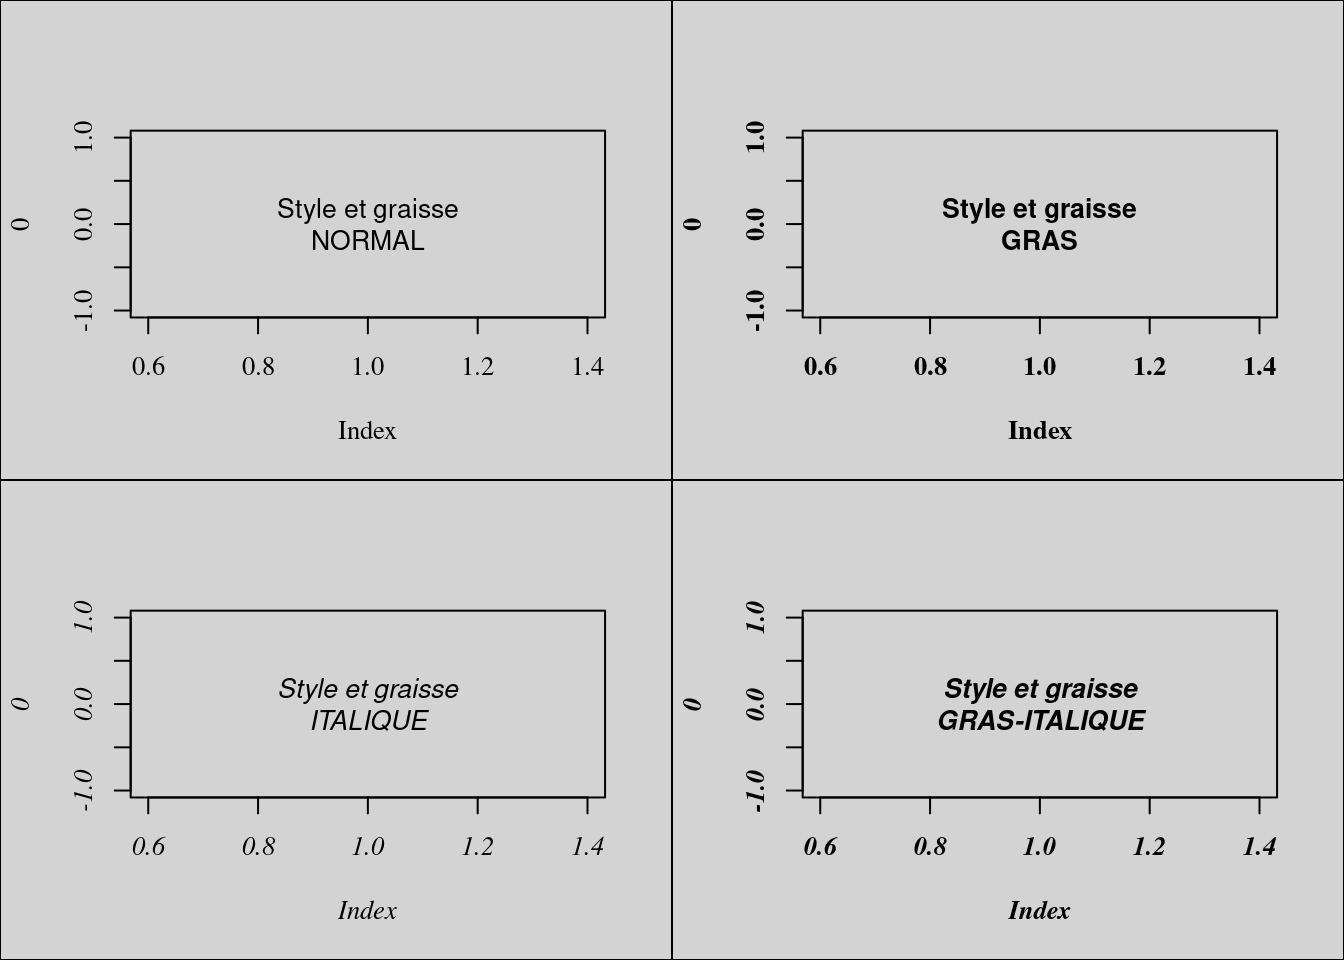
\includegraphics[width=0.6\linewidth]{visualiseR_files/figure-latex/unnamed-chunk-68-1} \end{center}

Dans les fonctions \texttt{text()} et \texttt{mtext()}, seul l'argument \texttt{font} est disponible.
De plus, tous ces paramètres auraient pu être modifiés dans le \texttt{par()} avant de
réaliser le graphique. Le corps de police se modifiera avec les arguments
\texttt{cex.axis}, \texttt{cex.lab}, \texttt{cex.main}, \texttt{cex.sub}. Attention : l'argument \texttt{cex}
modifie la taille des symboles ponctuels (sauf dans les fonctions \texttt{text()} et
\texttt{mtext()}). Regardons dans le \texttt{par()} les valeurs par défaut de chacun de ces
paramètres.

\begin{Shaded}
\begin{Highlighting}[]
\KeywordTok{par}\NormalTok{()[}\KeywordTok{grep}\NormalTok{(}\StringTok{"cex"}\NormalTok{, }\KeywordTok{names}\NormalTok{(}\KeywordTok{par}\NormalTok{()))]}
\CommentTok{#> $cex}
\CommentTok{#> [1] 1}
\CommentTok{#> }
\CommentTok{#> $cex.axis}
\CommentTok{#> [1] 1}
\CommentTok{#> }
\CommentTok{#> $cex.lab}
\CommentTok{#> [1] 1}
\CommentTok{#> }
\CommentTok{#> $cex.main}
\CommentTok{#> [1] 1.2}
\CommentTok{#> }
\CommentTok{#> $cex.sub}
\CommentTok{#> [1] 1}
\end{Highlighting}
\end{Shaded}

Modifions ces paramètres de corps de police.

\begin{Shaded}
\begin{Highlighting}[]
\KeywordTok{par}\NormalTok{(}\DataTypeTok{mfrow =} \KeywordTok{c}\NormalTok{(}\DecValTok{2}\NormalTok{, }\DecValTok{2}\NormalTok{), }\DataTypeTok{bg =} \StringTok{"lightgray"}\NormalTok{)}
\KeywordTok{plot}\NormalTok{(}\DecValTok{0}\NormalTok{, }\DataTypeTok{family =} \StringTok{"serif"}\NormalTok{, }\DataTypeTok{type =} \StringTok{"n"}\NormalTok{)}
\KeywordTok{text}\NormalTok{(}\DecValTok{1}\NormalTok{, }\DecValTok{0}\NormalTok{, }\StringTok{"Corps par défaut"}\NormalTok{, }\DataTypeTok{font =} \DecValTok{2}\NormalTok{)}
\KeywordTok{plot}\NormalTok{(}\DecValTok{0}\NormalTok{, }\DataTypeTok{family =} \StringTok{"serif"}\NormalTok{, }\DataTypeTok{type =} \StringTok{"n"}\NormalTok{, }\DataTypeTok{cex.lab =} \DecValTok{1}\NormalTok{, }\DataTypeTok{cex.axis =} \DecValTok{1}\NormalTok{)}
\KeywordTok{text}\NormalTok{(}\DecValTok{1}\NormalTok{, }\DecValTok{0}\NormalTok{, }\StringTok{"Corps de 1"}\NormalTok{, }\DataTypeTok{font =} \DecValTok{2}\NormalTok{, }\DataTypeTok{cex =} \DecValTok{1}\NormalTok{)}
\KeywordTok{plot}\NormalTok{(}\DecValTok{0}\NormalTok{, }\DataTypeTok{family =} \StringTok{"serif"}\NormalTok{, }\DataTypeTok{type =} \StringTok{"n"}\NormalTok{, }\DataTypeTok{cex.lab =} \DecValTok{2}\NormalTok{, }\DataTypeTok{cex.axis =} \DecValTok{2}\NormalTok{)}
\KeywordTok{text}\NormalTok{(}\DecValTok{1}\NormalTok{, }\DecValTok{0}\NormalTok{, }\StringTok{"Corps de 3"}\NormalTok{, }\DataTypeTok{font =} \DecValTok{2}\NormalTok{, }\DataTypeTok{cex =} \DecValTok{2}\NormalTok{)}
\KeywordTok{plot}\NormalTok{(}\DecValTok{0}\NormalTok{, }\DataTypeTok{family =} \StringTok{"serif"}\NormalTok{, }\DataTypeTok{type =} \StringTok{"n"}\NormalTok{, }\DataTypeTok{cex.lab =} \FloatTok{.35}\NormalTok{, }\DataTypeTok{cex.axis =} \FloatTok{.35}\NormalTok{)}
\KeywordTok{text}\NormalTok{(}\DecValTok{1}\NormalTok{, }\DecValTok{0}\NormalTok{, }\StringTok{"Corps de .35"}\NormalTok{, }\DataTypeTok{font =} \DecValTok{2}\NormalTok{, }\DataTypeTok{cex =} \FloatTok{.35}\NormalTok{)}
\end{Highlighting}
\end{Shaded}

\begin{center}\includegraphics[width=0.6\linewidth]{visualiseR_files/figure-latex/corps-1} \end{center}

Revenons maintenant aux polices de caractères. Il en existe deux autres sous R et celles-ci sont regroupées dans les fontes \texttt{Hershey}. Il s'agit des polices \texttt{script} (également appelée cursive) qui imite l'écriture manuscrite et \texttt{gothic} (ou fantaisie) avant tout décorative. Cet ensemble de fontes regroupe des polices permettant d'afficher toute sorte de symboles (grecs, musicaux, japonais, pictogrammes, etc.). Le meilleur moyen d'en faire le tour reste encore d'utiliser la commande suivante.

\begin{Shaded}
\begin{Highlighting}[]
\KeywordTok{demo}\NormalTok{(Hershey)}
\end{Highlighting}
\end{Shaded}

Regardons rapidement comment utiliser ces polices et caractères spéciaux.

\begin{Shaded}
\begin{Highlighting}[]
\KeywordTok{plot}\NormalTok{(}\DecValTok{0}\NormalTok{, }\DataTypeTok{type =} \StringTok{"n"}\NormalTok{, }\DataTypeTok{xlim =} \KeywordTok{c}\NormalTok{(}\DecValTok{1}\NormalTok{, }\DecValTok{4}\NormalTok{), }\DataTypeTok{ylim =} \KeywordTok{c}\NormalTok{(}\DecValTok{1}\NormalTok{, }\DecValTok{4}\NormalTok{), }\DataTypeTok{family =} \StringTok{"serif"}\NormalTok{)}
\KeywordTok{text}\NormalTok{(}\FloatTok{3.5}\NormalTok{, }\DecValTok{2}\NormalTok{, }\StringTok{" | CL"}\NormalTok{, }\DataTypeTok{vfont =} \KeywordTok{c}\NormalTok{(}\StringTok{"serif"}\NormalTok{, }\StringTok{"plain"}\NormalTok{), }\DataTypeTok{cex =} \DecValTok{2}\NormalTok{)}
\KeywordTok{text}\NormalTok{(}\FloatTok{1.5}\NormalTok{, }\DecValTok{2}\NormalTok{, }\StringTok{" | DI"}\NormalTok{, }\DataTypeTok{vfont =} \KeywordTok{c}\NormalTok{(}\StringTok{"serif"}\NormalTok{, }\StringTok{"plain"}\NormalTok{), }\DataTypeTok{cex =} \DecValTok{2}\NormalTok{, }\DataTypeTok{col =} \StringTok{"red"}\NormalTok{)}
\KeywordTok{text}\NormalTok{(}\FloatTok{1.5}\NormalTok{, }\DecValTok{3}\NormalTok{, }\StringTok{" | HE"}\NormalTok{, }\DataTypeTok{vfont =} \KeywordTok{c}\NormalTok{(}\StringTok{"serif"}\NormalTok{, }\StringTok{"plain"}\NormalTok{), }\DataTypeTok{cex =} \DecValTok{2}\NormalTok{, }\DataTypeTok{col =} \StringTok{"red"}\NormalTok{)}
\KeywordTok{text}\NormalTok{(}\FloatTok{3.5}\NormalTok{, }\DecValTok{3}\NormalTok{, }\StringTok{" | SP"}\NormalTok{, }\DataTypeTok{vfont =} \KeywordTok{c}\NormalTok{(}\StringTok{"serif"}\NormalTok{, }\StringTok{"plain"}\NormalTok{), }\DataTypeTok{cex =} \DecValTok{2}\NormalTok{)}
\KeywordTok{text}\NormalTok{(}\FloatTok{2.5}\NormalTok{, }\FloatTok{3.5}\NormalTok{, }\StringTok{"Police Gothique"}\NormalTok{,}
\DataTypeTok{vfont =} \KeywordTok{c}\NormalTok{(}\StringTok{"gothic english"}\NormalTok{, }\StringTok{"plain"}\NormalTok{))}
\KeywordTok{text}\NormalTok{(}\FloatTok{1.5}\NormalTok{, }\FloatTok{3.5}\NormalTok{, }\StringTok{" | #H2330"}\NormalTok{, }\DataTypeTok{vfont =} \KeywordTok{c}\NormalTok{(}\StringTok{"serif"}\NormalTok{, }\StringTok{"plain"}\NormalTok{), }\DataTypeTok{cex =} \DecValTok{2}\NormalTok{)}
\KeywordTok{text}\NormalTok{(}\FloatTok{3.5}\NormalTok{, }\FloatTok{3.5}\NormalTok{, }\StringTok{" | #H2331"}\NormalTok{, }\DataTypeTok{vfont =} \KeywordTok{c}\NormalTok{(}\StringTok{"serif"}\NormalTok{, }\StringTok{"plain"}\NormalTok{), }\DataTypeTok{cex =} \DecValTok{2}\NormalTok{)}
\KeywordTok{text}\NormalTok{(}\FloatTok{2.5}\NormalTok{, }\DecValTok{3}\NormalTok{, }\StringTok{" | *z"}\NormalTok{, }\DataTypeTok{vfont =} \KeywordTok{c}\NormalTok{(}\StringTok{"serif"}\NormalTok{, }\StringTok{"plain"}\NormalTok{), }\DataTypeTok{cex =} \DecValTok{2}\NormalTok{)}
\KeywordTok{text}\NormalTok{(}\FloatTok{2.5}\NormalTok{, }\DecValTok{2}\NormalTok{, }\StringTok{" | *p"}\NormalTok{, }\DataTypeTok{vfont =} \KeywordTok{c}\NormalTok{(}\StringTok{"serif"}\NormalTok{, }\StringTok{"plain"}\NormalTok{), }\DataTypeTok{cex =} \DecValTok{2}\NormalTok{)}
\KeywordTok{text}\NormalTok{(}\FloatTok{2.5}\NormalTok{, }\FloatTok{2.5}\NormalTok{, }\StringTok{"Police Script"}\NormalTok{,}
\DataTypeTok{vfont =} \KeywordTok{c}\NormalTok{(}\StringTok{"script"}\NormalTok{, }\StringTok{"italic"}\NormalTok{), }\DataTypeTok{srt =} \DecValTok{45}\NormalTok{)}
\KeywordTok{text}\NormalTok{(}\FloatTok{2.5}\NormalTok{, }\FloatTok{1.5}\NormalTok{, }\StringTok{"Police Symbol"}\NormalTok{,}
\DataTypeTok{vfont =} \KeywordTok{c}\NormalTok{(}\StringTok{"serif symbol"}\NormalTok{, }\StringTok{"bold"}\NormalTok{))}
\end{Highlighting}
\end{Shaded}

\begin{center}\includegraphics[width=0.6\linewidth]{visualiseR_files/figure-latex/hershey-1} \end{center}

Finalement, regardons comment ajouter des expressions mathématiques sur un graphe avec la fonction \texttt{expression}. N'hésitez pas à vous reporter aux rubriques d'aide de cette fonction et de la fonction \texttt{plotmath()} pour en savoir plus.

\begin{Shaded}
\begin{Highlighting}[]
\KeywordTok{plot}\NormalTok{(}\DecValTok{0}\NormalTok{, }\DataTypeTok{type =} \StringTok{"n"}\NormalTok{, }\DataTypeTok{xlim =} \KeywordTok{c}\NormalTok{(}\DecValTok{1}\NormalTok{, }\DecValTok{4}\NormalTok{), }\DataTypeTok{ylim =} \KeywordTok{c}\NormalTok{(}\DecValTok{1}\NormalTok{, }\DecValTok{4}\NormalTok{))}
\KeywordTok{text}\NormalTok{(}\FloatTok{2.5}\NormalTok{, }\FloatTok{2.5}\NormalTok{, }\KeywordTok{expression}\NormalTok{(}\KeywordTok{f}\NormalTok{(x) }\OperatorTok{==}\StringTok{ }\NormalTok{x}\OperatorTok{^}\DecValTok{2}\NormalTok{), }\DataTypeTok{cex =} \DecValTok{2}\NormalTok{)}
\KeywordTok{text}\NormalTok{(}\FloatTok{2.5}\NormalTok{, }\FloatTok{1.5}\NormalTok{, }\KeywordTok{expression}\NormalTok{(infinity), }\DataTypeTok{cex =} \DecValTok{2}\NormalTok{)}
\KeywordTok{text}\NormalTok{(}\FloatTok{2.5}\NormalTok{, }\FloatTok{3.5}\NormalTok{, }\KeywordTok{expression}\NormalTok{(}\KeywordTok{sqrt}\NormalTok{(x[i]) }\OperatorTok{>}\StringTok{ }\KeywordTok{bar}\NormalTok{(omega)), }\DataTypeTok{cex =} \DecValTok{2}\NormalTok{)}
\end{Highlighting}
\end{Shaded}

\begin{center}\includegraphics[width=0.5\linewidth]{visualiseR_files/figure-latex/mathexpr-1} \end{center}

\hypertarget{symboles-ponctuels}{%
\subsection{Symboles ponctuels}\label{symboles-ponctuels}}

Les points possèdent trois caractéristiques : un type de symbole, une taille et
une couleur. Le type de symbole est défini par l'argument \texttt{pch}, sa taille par
\texttt{cex}, et sa couleur par \texttt{col}. Modifions les deux derniers. Nous allons
incrémenter progressivement le symbole par défaut de R, et à chaque augmentation
de taille, on va attribuer une couleur différente, en respectant l'ordre des
couleurs dans l'arc-en-ciel.

\begin{Shaded}
\begin{Highlighting}[]
\NormalTok{k <-}\StringTok{ }\DecValTok{1}
\KeywordTok{plot}\NormalTok{(}\DecValTok{0}\NormalTok{, }\DataTypeTok{xlim =} \KeywordTok{c}\NormalTok{(}\DecValTok{1}\NormalTok{, }\DecValTok{4}\NormalTok{), }\DataTypeTok{ylim =} \KeywordTok{c}\NormalTok{(}\DecValTok{1}\NormalTok{, }\DecValTok{4}\NormalTok{), }\DataTypeTok{type =} \StringTok{"n"}\NormalTok{, }\DataTypeTok{ann =} \OtherTok{FALSE}\NormalTok{)}
\ControlFlowTok{for}\NormalTok{ (i }\ControlFlowTok{in} \KeywordTok{seq}\NormalTok{(.}\DecValTok{5}\NormalTok{, }\DecValTok{50}\NormalTok{, }\DataTypeTok{by =} \FloatTok{.5}\NormalTok{))\{}
\KeywordTok{points}\NormalTok{(}\FloatTok{2.5}\NormalTok{, }\FloatTok{2.5}\NormalTok{, }\DataTypeTok{cex =}\NormalTok{ i, }\DataTypeTok{col =} \KeywordTok{rainbow}\NormalTok{(}\DecValTok{120}\NormalTok{)[k])}
\NormalTok{k <-}\StringTok{ }\NormalTok{k }\OperatorTok{+}\StringTok{ }\DecValTok{1}
\NormalTok{\}}
\end{Highlighting}
\end{Shaded}

\begin{center}\includegraphics[width=0.5\linewidth]{visualiseR_files/figure-latex/unnamed-chunk-71-1} \end{center}

Attention, certains symboles sont caractérisés par deux couleurs : le contour et
le fond. L'argument \texttt{col} contrôlera la couleur de contour alors que l'argument
\texttt{bg} définira la couleur de fond. C'est le cas notamment des symboles 21 à 25.
La figure suivante illustre différentes valeurs possibles pour l'argument \texttt{pch}
qui contrôle le type de symbole. Notons que la valeur \textbf{1} sera différente de
la valeur \textbf{`1'}, la première affichant le premier symbole alors que le second
affichera la valeur 1.

\begin{center}\includegraphics[width=0.8\linewidth]{visualiseR_files/figure-latex/unnamed-chunk-72-1} \end{center}

Finalement, mentionnons qu'il est possible d'insérer des symboles \texttt{Hershey} via la fonction \texttt{text()}.

\begin{Shaded}
\begin{Highlighting}[]
\NormalTok{x <-}\StringTok{ }\KeywordTok{rnorm}\NormalTok{(}\DecValTok{50}\NormalTok{)}
\NormalTok{y <-}\StringTok{ }\KeywordTok{rnorm}\NormalTok{(}\DecValTok{50}\NormalTok{)}
\KeywordTok{plot}\NormalTok{(x, y, }\DataTypeTok{type =} \StringTok{"n"}\NormalTok{, }\DataTypeTok{ann =} \OtherTok{FALSE}\NormalTok{, }\DataTypeTok{bty =} \StringTok{"n"}\NormalTok{, }\DataTypeTok{las =} \DecValTok{1}\NormalTok{)}
\KeywordTok{text}\NormalTok{(x, y, }\StringTok{" | #H2330"}\NormalTok{, }\DataTypeTok{vfont =} \KeywordTok{c}\NormalTok{(}\StringTok{"serif"}\NormalTok{, }\StringTok{"plain"}\NormalTok{))}
\end{Highlighting}
\end{Shaded}

\begin{center}\includegraphics[width=0.5\linewidth]{visualiseR_files/figure-latex/unnamed-chunk-74-1} \end{center}

\hypertarget{types-de-lignes}{%
\subsection{Types de lignes}\label{types-de-lignes}}

Les lignes, tout comme les bordures de polygones et les axes, possèdent trois caractéristiques sur lesquelles on peut jouer : le type de ligne (\texttt{lty}), son épaisseur (\texttt{lwd}) et sa couleur (\texttt{col}). La figure suivante illustre ces différentes caractéristiques (inutile de détailler la couleur).

\begin{center}\includegraphics[width=0.8\linewidth]{visualiseR_files/figure-latex/unnamed-chunk-75-1} \end{center}

\hypertarget{modification-des-axes}{%
\subsection{Modification des axes}\label{modification-des-axes}}

Les axes sont un des éléments graphiques possédant probablement le plus grand nombre de paramètres modifiables. Et pour cause, c'est un élément clé pour la compréhension de l'information illustrée sur le graphique. Les arguments \texttt{cex.axis}, \texttt{col.axis}, \texttt{font.axis} ont déjà été abordés dans les sections précédentes. Nous n'y reviendrons pas.
Les arguments \texttt{xaxt} et \texttt{yaxt} vont contrôler l'affichage des axes : s'ils ont la valeur \textbf{`n'}, les axes ne seront pas affichés après l'appel à des fonctions de haut niveau graphique (e.g. \texttt{plot()}). Cela aura le même effet qu'utiliser l'argument \texttt{axes} de la fonction \texttt{plot()} et de lui attribuer la valeur \textbf{FALSE}. Mais, dans ce dernier cas, la boîte délimitant la région du plot ne sera pas affichée non plus.
Un autre argument peut être intéressant. Il s'agit de \texttt{mgp}. Celui-ci possède trois valeurs numériques qui vont contrôler le positionnement du nom des axes, des étiquettes des axes et des axes eux-même. Ces positions sont relatives à la délimitation de la région graphique.

\begin{Shaded}
\begin{Highlighting}[]
\KeywordTok{plot}\NormalTok{(}\DecValTok{0}\NormalTok{, }\DataTypeTok{pch =} \DecValTok{15}\NormalTok{, }\DataTypeTok{type =} \StringTok{"n"}\NormalTok{)}
\KeywordTok{text}\NormalTok{(}\DecValTok{1}\NormalTok{, }\DecValTok{0}\NormalTok{, }\StringTok{"Défaut"}\NormalTok{, }\DataTypeTok{font =} \DecValTok{2}\NormalTok{, }\DataTypeTok{cex =} \DecValTok{2}\NormalTok{)}
\KeywordTok{par}\NormalTok{(}\DataTypeTok{mgp =} \KeywordTok{c}\NormalTok{(}\DecValTok{0}\NormalTok{, }\DecValTok{1}\NormalTok{, }\DecValTok{0}\NormalTok{))}
\KeywordTok{plot}\NormalTok{(}\DecValTok{0}\NormalTok{, }\DataTypeTok{pch =} \DecValTok{15}\NormalTok{, }\DataTypeTok{type =} \StringTok{"n"}\NormalTok{)}
\KeywordTok{text}\NormalTok{(}\DecValTok{1}\NormalTok{, }\DecValTok{0}\NormalTok{, }\StringTok{"Modification}\CharTok{\textbackslash{}n}\StringTok{du nom des axes"}\NormalTok{, }\DataTypeTok{font =} \DecValTok{2}\NormalTok{, }\DataTypeTok{cex =} \DecValTok{2}\NormalTok{)}
\KeywordTok{par}\NormalTok{(}\DataTypeTok{mgp =} \KeywordTok{c}\NormalTok{(}\DecValTok{3}\NormalTok{, }\DecValTok{2}\NormalTok{, }\DecValTok{0}\NormalTok{))}
\KeywordTok{plot}\NormalTok{(}\DecValTok{0}\NormalTok{, }\DataTypeTok{pch =} \DecValTok{15}\NormalTok{, }\DataTypeTok{type =} \StringTok{"n"}\NormalTok{)}
\KeywordTok{text}\NormalTok{(}\DecValTok{1}\NormalTok{, }\DecValTok{0}\NormalTok{, }\StringTok{"Modification}\CharTok{\textbackslash{}n}\StringTok{des étiquettes"}\NormalTok{, }\DataTypeTok{font =} \DecValTok{2}\NormalTok{, }\DataTypeTok{cex =} \DecValTok{2}\NormalTok{)}
\KeywordTok{par}\NormalTok{(}\DataTypeTok{mgp =} \KeywordTok{c}\NormalTok{(}\DecValTok{3}\NormalTok{, }\DecValTok{1}\NormalTok{, }\FloatTok{-1.25}\NormalTok{))}
\KeywordTok{plot}\NormalTok{(}\DecValTok{0}\NormalTok{, }\DataTypeTok{pch =} \DecValTok{15}\NormalTok{, }\DataTypeTok{type =} \StringTok{"n"}\NormalTok{)}
\KeywordTok{text}\NormalTok{(}\DecValTok{1}\NormalTok{, }\DecValTok{0}\NormalTok{, }\StringTok{"Modification}\CharTok{\textbackslash{}n}\StringTok{des axes"}\NormalTok{, }\DataTypeTok{font =} \DecValTok{2}\NormalTok{, }\DataTypeTok{cex =} \DecValTok{2}\NormalTok{)}
\end{Highlighting}
\end{Shaded}

\begin{center}\includegraphics[width=0.5\linewidth]{visualiseR_files/figure-latex/unnamed-chunk-76-1} \end{center}

Le tableau suivant liste les paramètres graphiques se rapportant aux axes qu'il est intéressant de connaître.

\begin{longtable}[]{@{}llll@{}}
\caption{Arguments de \texttt{par()}}\tabularnewline
\toprule
\textbf{Argument} & \textbf{Signification} & \texttt{par()} & \textbf{À la volée}\tabularnewline
\midrule
\endfirsthead
\toprule
\textbf{Argument} & \textbf{Signification} & \texttt{par()} & \textbf{À la volée}\tabularnewline
\midrule
\endhead
\texttt{ann} & Contrôle la présence du nom des axes & x & x\tabularnewline
\texttt{axes} & \textbf{TRUE} ou \textbf{FALSE} (pas d'axes ni de boîte) & \& x &\tabularnewline
\texttt{cex.axis} & Taille de caractères des étiquettes des axes & x & x\tabularnewline
\texttt{cex.lab} & Taille de caractères du nom des axes & x & x\tabularnewline
\texttt{col.axis} & Couleur des axes et de leurs étiquettes & x & x\tabularnewline
\texttt{col.lab} & Couleur du nom des axes & x & x\tabularnewline
\texttt{col.ticks} & Couleur de la graduation & \& x &\tabularnewline
\texttt{font.axis} & Style et graisse des étiquettes & x & x\tabularnewline
\texttt{font.lab} & Style et graisse du nom des axes & x & x\tabularnewline
\texttt{las} & Orientation des étiquettes des axes (\textbf{0}, \textbf{1}, \textbf{2}, \textbf{3}) & x & x\tabularnewline
\texttt{mgp} & Voir page précédente & x &\tabularnewline
\texttt{tck} & Longueur de la graduation & x & x\tabularnewline
\texttt{tick} & \textbf{TRUE} ou \textbf{FALSE} (pas de graduation) & \& x &\tabularnewline
\texttt{lty} & Type de tracé des axes & x & x\tabularnewline
\texttt{lty.ticks} & Type de tracé de la graduation & \& x &\tabularnewline
\texttt{lwd} & Épaisseur des axes & x & x\tabularnewline
\texttt{lwd.ticks} & Épaisseur de la graduation & \& x &\tabularnewline
\texttt{xaxp} & Nombre de graduation en abscisse & x & x\tabularnewline
\texttt{xaxs} & \textbf{`r'} (ajout de 4\% aux limites de l'axe) ou \textbf{`i'} & x & x\tabularnewline
\texttt{xaxt} & \textbf{TRUE} ou \textbf{FALSE} (pas d'axe des x) & x & x\tabularnewline
\texttt{xlab} & Nom de l'axe des x & \& x &\tabularnewline
\texttt{xlim} & Étendue de l'axe des x & \& x &\tabularnewline
\texttt{yaxp} & Nombre de graduation en ordonnée & x & x\tabularnewline
\texttt{yaxs} & Voir \texttt{xaxs} & x & x\tabularnewline
\texttt{yaxt} & Voir \texttt{xaxt} & x & x\tabularnewline
\texttt{ylab} & Nom de l'axe des y & \& x &\tabularnewline
\texttt{ylim} & Étendue de l'axe des y & \& x &\tabularnewline
\bottomrule
\end{longtable}

Une modification à la volée signifie que le paramètre en question verra sa valeur par défaut changée dans les fonctions graphiques telles que \texttt{plot()}, \texttt{axis()}, etc. Le paramètre \texttt{las} pourra prendre les valeurs :

\begin{itemize}
\tightlist
\item
  \texttt{las\ =\ 0} : étiquettes parallèles aux axes;
\item
  \texttt{las\ =\ 1} : étiquettes horizontales;
\item
  \texttt{las\ =\ 2} : étiquettes perpendiculaires aux axes;
\item
  \texttt{las\ =\ 3} : étiquettes verticales.
\end{itemize}

Pour terminer, regardons un exemple faisant appel à certains de ces paramètres graphiques.

\begin{Shaded}
\begin{Highlighting}[]
\CommentTok{## Empty plot}
\KeywordTok{par}\NormalTok{(}\DataTypeTok{mgp =} \KeywordTok{c}\NormalTok{(}\FloatTok{1.75}\NormalTok{, }\FloatTok{0.75}\NormalTok{, }\DecValTok{0}\NormalTok{))}
\KeywordTok{plot}\NormalTok{(}\DecValTok{0}\NormalTok{, }\DataTypeTok{type =} \StringTok{"n"}\NormalTok{, }\DataTypeTok{xlim =} \KeywordTok{c}\NormalTok{(}\DecValTok{0}\NormalTok{, }\DecValTok{40}\NormalTok{), }\DataTypeTok{ylim =} \KeywordTok{c}\NormalTok{(}\DecValTok{0}\NormalTok{, }\DecValTok{40}\NormalTok{), }\DataTypeTok{axes =} \OtherTok{FALSE}\NormalTok{, }\DataTypeTok{ann =} \OtherTok{FALSE}\NormalTok{, }\DataTypeTok{xaxs =} \StringTok{"i"}\NormalTok{, }\DataTypeTok{yaxs =} \StringTok{"i"}\NormalTok{)}
\CommentTok{## Background}
\KeywordTok{rect}\NormalTok{(}\DecValTok{0}\NormalTok{, }\DecValTok{0}\NormalTok{, }\DecValTok{40}\NormalTok{, }\DecValTok{40}\NormalTok{, }\DataTypeTok{col =} \StringTok{"gray"}\NormalTok{, }\DataTypeTok{border =} \StringTok{"darkgray"}\NormalTok{, }\DataTypeTok{lwd =} \DecValTok{3}\NormalTok{)}
\ControlFlowTok{for}\NormalTok{ (i }\ControlFlowTok{in} \KeywordTok{seq}\NormalTok{(}\DecValTok{10}\NormalTok{, }\DecValTok{30}\NormalTok{, }\DecValTok{10}\NormalTok{))\{}
  \KeywordTok{points}\NormalTok{(}\KeywordTok{c}\NormalTok{(}\DecValTok{0}\NormalTok{, }\DecValTok{40}\NormalTok{), }\KeywordTok{c}\NormalTok{(i, i), }\DataTypeTok{col =} \StringTok{"white"}\NormalTok{, }\DataTypeTok{type =} \StringTok{"l"}\NormalTok{)}
  \KeywordTok{points}\NormalTok{(}\KeywordTok{c}\NormalTok{(i, i), }\KeywordTok{c}\NormalTok{(}\DecValTok{0}\NormalTok{, }\DecValTok{40}\NormalTok{), }\DataTypeTok{col =} \StringTok{"white"}\NormalTok{, }\DataTypeTok{type =} \StringTok{"l"}\NormalTok{)}
\NormalTok{\}}
\ControlFlowTok{for}\NormalTok{ (i }\ControlFlowTok{in} \KeywordTok{seq}\NormalTok{(}\DecValTok{5}\NormalTok{, }\DecValTok{35}\NormalTok{, }\DecValTok{10}\NormalTok{))\{}
  \KeywordTok{points}\NormalTok{(}\KeywordTok{c}\NormalTok{(}\DecValTok{0}\NormalTok{, }\DecValTok{40}\NormalTok{), }\KeywordTok{c}\NormalTok{(i, i), }\DataTypeTok{col =} \StringTok{"white"}\NormalTok{, }\DataTypeTok{type =} \StringTok{"l"}\NormalTok{, }\DataTypeTok{lty =} \DecValTok{3}\NormalTok{)}
  \KeywordTok{points}\NormalTok{(}\KeywordTok{c}\NormalTok{(i, i), }\KeywordTok{c}\NormalTok{(}\DecValTok{0}\NormalTok{, }\DecValTok{40}\NormalTok{), }\DataTypeTok{col =} \StringTok{"white"}\NormalTok{, }\DataTypeTok{type =} \StringTok{"l"}\NormalTok{, }\DataTypeTok{lty =} \DecValTok{3}\NormalTok{)}
\NormalTok{\}}
\CommentTok{## Axes principaux}
\KeywordTok{axis}\NormalTok{(}\DataTypeTok{side =} \DecValTok{1}\NormalTok{, }\DataTypeTok{at =} \KeywordTok{seq}\NormalTok{(}\DecValTok{0}\NormalTok{, }\DecValTok{40}\NormalTok{, }\DataTypeTok{by =} \DecValTok{10}\NormalTok{), }\DataTypeTok{labels =} \KeywordTok{seq}\NormalTok{(}\DecValTok{0}\NormalTok{, }\DecValTok{40}\NormalTok{, }\DataTypeTok{by =} \DecValTok{10}\NormalTok{), }\DataTypeTok{lwd =} \DecValTok{0}\NormalTok{, }\DataTypeTok{pos =} \DecValTok{0}\NormalTok{, }\DataTypeTok{lwd.ticks =} \DecValTok{1}\NormalTok{,}
\DataTypeTok{col =} \StringTok{"darkgray"}\NormalTok{, }\DataTypeTok{family =} \StringTok{"serif"}\NormalTok{, }\DataTypeTok{col.axis =} \StringTok{"darkgray"}\NormalTok{)}
\KeywordTok{axis}\NormalTok{(}\DataTypeTok{side =} \DecValTok{2}\NormalTok{, }\DataTypeTok{at =} \KeywordTok{seq}\NormalTok{(}\DecValTok{0}\NormalTok{, }\DecValTok{40}\NormalTok{, }\DataTypeTok{by =} \DecValTok{10}\NormalTok{), }\DataTypeTok{labels =} \KeywordTok{seq}\NormalTok{(}\DecValTok{0}\NormalTok{, }\DecValTok{40}\NormalTok{, }\DataTypeTok{by =} \DecValTok{10}\NormalTok{), }\DataTypeTok{lwd =} \DecValTok{0}\NormalTok{, }\DataTypeTok{pos =} \DecValTok{0}\NormalTok{, }\DataTypeTok{lwd.ticks =} \DecValTok{1}\NormalTok{,}
\DataTypeTok{col =} \StringTok{"darkgray"}\NormalTok{, }\DataTypeTok{family =} \StringTok{"serif"}\NormalTok{, }\DataTypeTok{las =} \DecValTok{2}\NormalTok{, }\DataTypeTok{col.axis =} \StringTok{"darkgray"}\NormalTok{)}
\CommentTok{## Axes secondaires}
\KeywordTok{axis}\NormalTok{(}\DataTypeTok{side =} \DecValTok{1}\NormalTok{, }\DataTypeTok{at =} \KeywordTok{seq}\NormalTok{(}\DecValTok{5}\NormalTok{, }\DecValTok{35}\NormalTok{, }\DataTypeTok{by =} \DecValTok{10}\NormalTok{), }\DataTypeTok{labels =} \OtherTok{FALSE}\NormalTok{, }\DataTypeTok{lwd =} \DecValTok{0}\NormalTok{, }\DataTypeTok{pos =} \DecValTok{0}\NormalTok{, }\DataTypeTok{tck =} \FloatTok{-0.01}\NormalTok{, }\DataTypeTok{lwd.ticks =} \DecValTok{1}\NormalTok{,}
\DataTypeTok{col.ticks =} \StringTok{"darkgray"}\NormalTok{)}
\KeywordTok{axis}\NormalTok{(}\DataTypeTok{side =} \DecValTok{2}\NormalTok{, }\DataTypeTok{at =} \KeywordTok{seq}\NormalTok{(}\DecValTok{5}\NormalTok{, }\DecValTok{35}\NormalTok{, }\DataTypeTok{by =} \DecValTok{10}\NormalTok{), }\DataTypeTok{labels =} \OtherTok{FALSE}\NormalTok{, }\DataTypeTok{lwd =} \DecValTok{0}\NormalTok{, }\DataTypeTok{pos =} \DecValTok{0}\NormalTok{, }\DataTypeTok{tck =} \FloatTok{-0.01}\NormalTok{, }\DataTypeTok{lwd.ticks =} \DecValTok{1}\NormalTok{,}
\DataTypeTok{col.ticks =} \StringTok{"darkgray"}\NormalTok{)}
\CommentTok{## Nom des axes}
\KeywordTok{mtext}\NormalTok{(}\DataTypeTok{text =} \StringTok{"x-axis"}\NormalTok{, }\DataTypeTok{side =} \DecValTok{1}\NormalTok{, }\DataTypeTok{line =} \FloatTok{1.5}\NormalTok{, }\DataTypeTok{family =} \StringTok{"serif"}\NormalTok{, }\DataTypeTok{font =} \DecValTok{2}\NormalTok{, }\DataTypeTok{col =} \StringTok{"darkgray"}\NormalTok{)}
\KeywordTok{mtext}\NormalTok{(}\DataTypeTok{text =} \StringTok{"y-axis"}\NormalTok{, }\DataTypeTok{side =} \DecValTok{2}\NormalTok{, }\DataTypeTok{line =} \FloatTok{1.75}\NormalTok{, }\DataTypeTok{family =} \StringTok{"serif"}\NormalTok{, }\DataTypeTok{las =} \DecValTok{0}\NormalTok{, }\DataTypeTok{font =} \DecValTok{2}\NormalTok{, }\DataTypeTok{col =} \StringTok{"darkgray"}\NormalTok{)}
\CommentTok{## Informations}
\NormalTok{x <-}\StringTok{ }\KeywordTok{sample}\NormalTok{(}\DecValTok{1}\OperatorTok{:}\DecValTok{39}\NormalTok{, }\DecValTok{50}\NormalTok{, }\DataTypeTok{replace =} \OtherTok{TRUE}\NormalTok{)}
\NormalTok{y <-}\StringTok{ }\KeywordTok{sample}\NormalTok{(}\DecValTok{1}\OperatorTok{:}\DecValTok{39}\NormalTok{, }\DecValTok{50}\NormalTok{, }\DataTypeTok{replace =} \OtherTok{TRUE}\NormalTok{)}
\KeywordTok{points}\NormalTok{(x, y, }\DataTypeTok{col =} \StringTok{"#FF000080"}\NormalTok{, }\DataTypeTok{pch =} \DecValTok{19}\NormalTok{, }\DataTypeTok{cex =} \DecValTok{2}\NormalTok{)}
\end{Highlighting}
\end{Shaded}

\begin{center}\includegraphics[width=0.8\linewidth]{visualiseR_files/figure-latex/unnamed-chunk-78-1} \end{center}

\hypertarget{ajustement-des-marges}{%
\subsection{Ajustement des marges}\label{ajustement-des-marges}}

Les marges sont également une notion importante d'un graphique. Plusieurs paramètres graphiques permettent de les contrôler. Nous n'en verrons que deux : \texttt{oma} (pour \emph{outer margin}) et \texttt{mar} (pour \emph{figure margin}). Regardons à quoi elles correspondent au travers de deux exemples.

\begin{Shaded}
\begin{Highlighting}[]
\KeywordTok{par}\NormalTok{(}\DataTypeTok{oma =} \KeywordTok{c}\NormalTok{(}\DecValTok{2}\NormalTok{, }\DecValTok{2}\NormalTok{, }\DecValTok{2}\NormalTok{, }\DecValTok{2}\NormalTok{), }\DataTypeTok{bg =} \StringTok{"lightgray"}\NormalTok{, }\DataTypeTok{family =} \StringTok{"mono"}\NormalTok{)}
\KeywordTok{plot}\NormalTok{(}\DecValTok{0}\NormalTok{, }\DecValTok{0}\NormalTok{, }\DataTypeTok{type =} \StringTok{"n"}\NormalTok{, }\DataTypeTok{xlab =} \StringTok{"Axe des x"}\NormalTok{, }\DataTypeTok{ylab =} \StringTok{"Axe des y"}\NormalTok{)}
\KeywordTok{box}\NormalTok{(}\StringTok{"plot"}\NormalTok{, }\DataTypeTok{col =} \StringTok{"red"}\NormalTok{, }\DataTypeTok{lwd =} \DecValTok{2}\NormalTok{)}
\KeywordTok{rect}\NormalTok{(}\OperatorTok{-}\DecValTok{1}\NormalTok{, }\DecValTok{-1}\NormalTok{, }\DecValTok{1}\NormalTok{, }\DecValTok{1}\NormalTok{, }\DataTypeTok{border =} \OtherTok{NA}\NormalTok{, }\DataTypeTok{col =} \StringTok{"red"}\NormalTok{, }\DataTypeTok{density =} \DecValTok{20}\NormalTok{, }\DataTypeTok{angle =} \DecValTok{45}\NormalTok{)}
\KeywordTok{box}\NormalTok{(}\StringTok{"figure"}\NormalTok{, }\DataTypeTok{col =} \StringTok{"blue"}\NormalTok{, }\DataTypeTok{lwd =} \DecValTok{2}\NormalTok{)}
\KeywordTok{box}\NormalTok{(}\StringTok{"outer"}\NormalTok{, }\DataTypeTok{col =} \StringTok{"darkgreen"}\NormalTok{, }\DataTypeTok{lwd =} \DecValTok{4}\NormalTok{)}
\KeywordTok{mtext}\NormalTok{(}\DataTypeTok{side =} \DecValTok{2}\NormalTok{, }\DataTypeTok{line =} \FloatTok{4.75}\NormalTok{, }\DataTypeTok{text =} \StringTok{"oma"}\NormalTok{, }\DataTypeTok{col =} \StringTok{"darkgreen"}\NormalTok{, }\DataTypeTok{font =} \DecValTok{2}\NormalTok{)}
\KeywordTok{mtext}\NormalTok{(}\DataTypeTok{side =} \DecValTok{3}\NormalTok{, }\DataTypeTok{line =} \FloatTok{1.5}\NormalTok{, }\DataTypeTok{text =} \StringTok{"mar"}\NormalTok{, }\DataTypeTok{col =} \StringTok{"blue"}\NormalTok{, }\DataTypeTok{font =} \DecValTok{2}\NormalTok{)}
\end{Highlighting}
\end{Shaded}

\begin{center}\includegraphics[width=0.5\linewidth]{visualiseR_files/figure-latex/unnamed-chunk-80-1} \end{center}

\begin{Shaded}
\begin{Highlighting}[]
\KeywordTok{par}\NormalTok{(}\DataTypeTok{oma =} \KeywordTok{c}\NormalTok{(}\DecValTok{2}\NormalTok{, }\DecValTok{2}\NormalTok{, }\DecValTok{2}\NormalTok{, }\DecValTok{2}\NormalTok{), }\DataTypeTok{bg =} \StringTok{"lightgray"}\NormalTok{, }\DataTypeTok{mfrow =} \KeywordTok{c}\NormalTok{(}\DecValTok{1}\NormalTok{, }\DecValTok{2}\NormalTok{))}
\KeywordTok{par}\NormalTok{(}\DataTypeTok{family =} \StringTok{"mono"}\NormalTok{)}
\KeywordTok{plot}\NormalTok{(}\DecValTok{0}\NormalTok{, }\DecValTok{0}\NormalTok{, }\DataTypeTok{type =} \StringTok{"n"}\NormalTok{, }\DataTypeTok{xlab =} \StringTok{"Axe des x"}\NormalTok{, }\DataTypeTok{ylab =} \StringTok{"Axe des y"}\NormalTok{)}
\KeywordTok{box}\NormalTok{(}\StringTok{"plot"}\NormalTok{, }\DataTypeTok{col =} \StringTok{"red"}\NormalTok{, }\DataTypeTok{lwd =} \DecValTok{2}\NormalTok{)}
\KeywordTok{rect}\NormalTok{(}\OperatorTok{-}\DecValTok{1}\NormalTok{, }\DecValTok{-1}\NormalTok{, }\DecValTok{1}\NormalTok{, }\DecValTok{1}\NormalTok{, }\DataTypeTok{border =} \OtherTok{NA}\NormalTok{, }\DataTypeTok{col =} \StringTok{"red"}\NormalTok{, }\DataTypeTok{density =} \DecValTok{20}\NormalTok{, }\DataTypeTok{angle =} \DecValTok{45}\NormalTok{)}
\KeywordTok{box}\NormalTok{(}\StringTok{"figure"}\NormalTok{, }\DataTypeTok{col =} \StringTok{"blue"}\NormalTok{, }\DataTypeTok{lwd =} \DecValTok{2}\NormalTok{)}
\KeywordTok{mtext}\NormalTok{(}\DataTypeTok{side =} \DecValTok{3}\NormalTok{, }\DataTypeTok{line =} \FloatTok{1.75}\NormalTok{, }\DataTypeTok{text =} \StringTok{"mar"}\NormalTok{, }\DataTypeTok{col =} \StringTok{"blue"}\NormalTok{, }\DataTypeTok{font =} \DecValTok{2}\NormalTok{)}
\KeywordTok{plot}\NormalTok{(}\DecValTok{0}\NormalTok{, }\DecValTok{0}\NormalTok{, }\DataTypeTok{type =} \StringTok{"n"}\NormalTok{, }\DataTypeTok{xlab =} \StringTok{"Axe des x"}\NormalTok{, }\DataTypeTok{ylab =} \StringTok{"Axe des y"}\NormalTok{)}
\KeywordTok{box}\NormalTok{(}\StringTok{"plot"}\NormalTok{, }\DataTypeTok{col =} \StringTok{"red"}\NormalTok{, }\DataTypeTok{lwd =} \DecValTok{2}\NormalTok{)}
\KeywordTok{rect}\NormalTok{(}\OperatorTok{-}\DecValTok{1}\NormalTok{, }\DecValTok{-1}\NormalTok{, }\DecValTok{1}\NormalTok{, }\DecValTok{1}\NormalTok{, }\DataTypeTok{border =} \OtherTok{NA}\NormalTok{, }\DataTypeTok{col =} \StringTok{"red"}\NormalTok{, }\DataTypeTok{density =} \DecValTok{20}\NormalTok{, }\DataTypeTok{angle =} \DecValTok{45}\NormalTok{)}
\KeywordTok{box}\NormalTok{(}\StringTok{"figure"}\NormalTok{, }\DataTypeTok{col =} \StringTok{"blue"}\NormalTok{, }\DataTypeTok{lwd =} \DecValTok{2}\NormalTok{)}
\KeywordTok{mtext}\NormalTok{(}\DataTypeTok{side =} \DecValTok{3}\NormalTok{, }\DataTypeTok{line =} \FloatTok{1.75}\NormalTok{, }\DataTypeTok{text =} \StringTok{"mar"}\NormalTok{, }\DataTypeTok{col =} \StringTok{"blue"}\NormalTok{, }\DataTypeTok{font =} \DecValTok{2}\NormalTok{)}
\KeywordTok{box}\NormalTok{(}\StringTok{"outer"}\NormalTok{, }\DataTypeTok{col =} \StringTok{"darkgreen"}\NormalTok{, }\DataTypeTok{lwd =} \DecValTok{4}\NormalTok{)}
\KeywordTok{mtext}\NormalTok{(}\DataTypeTok{side =} \DecValTok{3}\NormalTok{, }\DataTypeTok{line =} \FloatTok{0.5}\NormalTok{, }\DataTypeTok{text =} \StringTok{"oma"}\NormalTok{, }\DataTypeTok{col =} \StringTok{"darkgreen"}\NormalTok{, }\DataTypeTok{font =} \DecValTok{2}\NormalTok{, }\DataTypeTok{outer =} \OtherTok{TRUE}\NormalTok{)}
\end{Highlighting}
\end{Shaded}

\begin{center}\includegraphics[width=0.6\linewidth]{visualiseR_files/figure-latex/unnamed-chunk-82-1} \end{center}

L'espace compris entre les bordures verte et bleue correspond à la marge
extérieure à la région graphique (\emph{outer margin}). Elle est contrôlée par le
paramètre \texttt{oma}. Par défaut, sa valeur est :

\begin{Shaded}
\begin{Highlighting}[]
\KeywordTok{par}\NormalTok{()}\OperatorTok{$}\NormalTok{oma}
\CommentTok{#> [1] 0 0 0 0}
\end{Highlighting}
\end{Shaded}

Ces quatre chiffres correspondent respectivement aux marges en bas, à gauche, en haut et à droite. Comme on peut le voir sur la figure 3.13, ce paramètre peut être intéressant à ajuster dans le cas d'une figure composite. En effet, il permettra de définir des marges communes à tous les graphes de la figure.
L'argument \texttt{mar}, quant à lui, contrôle la taille de la région du plot (excluant les axes). Son ajustement est donc très important. Par défaut, il vaut :

\begin{Shaded}
\begin{Highlighting}[]
\KeywordTok{par}\NormalTok{()}\OperatorTok{$}\NormalTok{mar}
\CommentTok{#> [1] 5.1 4.1 4.1 2.1}
\end{Highlighting}
\end{Shaded}

La marge du bas est destinée à accueillir à la fois le nom de l'axe des x et un sous-titre : pour cela, sa valeur est plus importante que les autres marges. Notamment, la marge de droite, qui par défaut, ne contiendra aucun élément.
Il n'existe pas de règle absolue concernant ce paramètre : la conception graphique de la figure guidera sa définition.

\begin{Shaded}
\begin{Highlighting}[]
\KeywordTok{par}\NormalTok{(}\DataTypeTok{mfrow =} \KeywordTok{c}\NormalTok{(}\DecValTok{2}\NormalTok{, }\DecValTok{2}\NormalTok{), }\DataTypeTok{bg =} \StringTok{"lightgray"}\NormalTok{, }\DataTypeTok{family =} \StringTok{"serif"}\NormalTok{)}
\KeywordTok{plot}\NormalTok{(}\DecValTok{0}\NormalTok{, }\DataTypeTok{pch =} \DecValTok{15}\NormalTok{, }\DataTypeTok{main =} \StringTok{"'mar' par défaut"}\NormalTok{)}
\KeywordTok{box}\NormalTok{(}\StringTok{"figure"}\NormalTok{, }\DataTypeTok{lwd =} \DecValTok{2}\NormalTok{)}
\KeywordTok{box}\NormalTok{(}\StringTok{"plot"}\NormalTok{, }\DataTypeTok{col =} \StringTok{"red"}\NormalTok{, }\DataTypeTok{lwd =} \DecValTok{2}\NormalTok{)}
\KeywordTok{par}\NormalTok{(}\DataTypeTok{mar =} \KeywordTok{c}\NormalTok{(}\DecValTok{8}\NormalTok{, }\DecValTok{8}\NormalTok{, }\DecValTok{8}\NormalTok{, }\DecValTok{8}\NormalTok{))}
\KeywordTok{plot}\NormalTok{(}\DecValTok{0}\NormalTok{, }\DataTypeTok{pch =} \DecValTok{15}\NormalTok{, }\DataTypeTok{main =} \StringTok{"'mar' = c(8, 8, 8, 8)"}\NormalTok{)}
\KeywordTok{box}\NormalTok{(}\StringTok{"figure"}\NormalTok{, }\DataTypeTok{lwd =} \DecValTok{2}\NormalTok{)}
\KeywordTok{box}\NormalTok{(}\StringTok{"plot"}\NormalTok{, }\DataTypeTok{col =} \StringTok{"red"}\NormalTok{, }\DataTypeTok{lwd =} \DecValTok{2}\NormalTok{)}
\KeywordTok{par}\NormalTok{(}\DataTypeTok{mar =} \KeywordTok{c}\NormalTok{(}\DecValTok{2}\NormalTok{, }\DecValTok{2}\NormalTok{, }\DecValTok{2}\NormalTok{, }\DecValTok{2}\NormalTok{))}
\KeywordTok{plot}\NormalTok{(}\DecValTok{0}\NormalTok{, }\DataTypeTok{pch =} \DecValTok{15}\NormalTok{, }\DataTypeTok{main =} \StringTok{"'mar' = c(2, 2, 2, 2)"}\NormalTok{)}
\KeywordTok{box}\NormalTok{(}\StringTok{"figure"}\NormalTok{, }\DataTypeTok{lwd =} \DecValTok{2}\NormalTok{)}
\KeywordTok{box}\NormalTok{(}\StringTok{"plot"}\NormalTok{, }\DataTypeTok{col =} \StringTok{"red"}\NormalTok{, }\DataTypeTok{lwd =} \DecValTok{2}\NormalTok{)}
\KeywordTok{par}\NormalTok{(}\DataTypeTok{mar =} \KeywordTok{c}\NormalTok{(}\DecValTok{1}\NormalTok{, }\DecValTok{1}\NormalTok{, }\DecValTok{1}\NormalTok{, }\DecValTok{1}\NormalTok{))}
\KeywordTok{plot}\NormalTok{(}\DecValTok{0}\NormalTok{, }\DataTypeTok{pch =} \DecValTok{15}\NormalTok{, }\DataTypeTok{main =} \StringTok{"'mar' = c(1, 1, 1, 1)"}\NormalTok{)}
\KeywordTok{box}\NormalTok{(}\StringTok{"figure"}\NormalTok{, }\DataTypeTok{lwd =} \DecValTok{2}\NormalTok{)}
\KeywordTok{box}\NormalTok{(}\StringTok{"plot"}\NormalTok{, }\DataTypeTok{col =} \StringTok{"red"}\NormalTok{, }\DataTypeTok{lwd =} \DecValTok{2}\NormalTok{)}
\end{Highlighting}
\end{Shaded}

\begin{center}\includegraphics[width=0.6\linewidth]{visualiseR_files/figure-latex/unnamed-chunk-86-1} \end{center}

\hypertarget{les-couleurs-sous-r}{%
\subsection{Les couleurs sous R}\label{les-couleurs-sous-r}}

Terminons ce chapitre par les couleurs. C'est un domaine très vaste. En
informatique, il existe plusieurs systèmes de représentation des couleurs. On
peut utiliser des palettes de couleurs prédéfinies, le système Rouge-Vert-Bleu,
RVB (ou \emph{RGB} en anglais) ou encore le système hexadécimal. D'autres systèmes
existent, mais nous ne les verrons pas aujourd'hui. Commençons par le plus
simple : les palettes. R dispose d'une palette de base dans laquelle figurent
huit couleurs prédéfinies.

\begin{Shaded}
\begin{Highlighting}[]
\KeywordTok{palette}\NormalTok{()}
\CommentTok{#> [1] "black"   "#DF536B" "#61D04F" "#2297E6" "#28E2E5" "#CD0BBC" "#F5C710"}
\CommentTok{#> [8] "gray62"}
\end{Highlighting}
\end{Shaded}

Cette palette, bien que peu garnie, est intéressante, car elle permet de choisir une couleur par son nom ou par sa position dans le vecteur \texttt{palette()}. Outre cette palette, R met à notre disposition la palette \texttt{colors()} qui comporte 657 couleurs, chacune avec un nom.

\begin{Shaded}
\begin{Highlighting}[]
\KeywordTok{colors}\NormalTok{()[}\DecValTok{1}\OperatorTok{:}\DecValTok{8}\NormalTok{]}
\CommentTok{#> [1] "white"         "aliceblue"     "antiquewhite"  "antiquewhite1"}
\CommentTok{#> [5] "antiquewhite2" "antiquewhite3" "antiquewhite4" "aquamarine"}
\end{Highlighting}
\end{Shaded}

D'autres palettes existent sous R, mais nous en parlerons plus loin, car nous
devons voir avant certaines notions importantes de colorimétrie.
Qu'est-ce-qu'une couleur ? En informatique, on utilise souvent (mais pas tout le
temps) la synthèse additive des trois couleurs primaires : Rouge-Vert-Bleu. Dans
ce système, 100\% de rouge, 100\% de vert et 100\% de bleu donnera du blanc. En
quantités égales, on obtiendra du gris dont la teinte dépendra de la quantité de
couleur. Les valeurs de chaque couleur primaire s'étalonnent de 0 à 1 (100\%) ou
de 0 à 255.

\begin{longtable}[]{@{}llll@{}}
\toprule
\textbf{Nom} & \textbf{Rouge} & \textbf{Vert} & \textbf{Bleu}\tabularnewline
\midrule
\endhead
Rouge & 100\% & 0\% & 0\%\tabularnewline
Bleu & 0\% & 0\% & 100\%\tabularnewline
Vert & 0\% & 100\% & 0\%\tabularnewline
Noir & 0\% & 0\% & 0\%\tabularnewline
Blanc & 100\% & 100\% & 100\%\tabularnewline
Gris clair & 80\% & 80\% & 80\%\tabularnewline
Gris foncé & 20\% & 20\% & 20\%\tabularnewline
Cyan & 0\% & 100\% & 100\%\tabularnewline
Magenta & 100\% & 0\% & 100\%\tabularnewline
Jaune & 100\% & 100\% & 0\%\tabularnewline
\bottomrule
\end{longtable}

La fonction \texttt{rgb()} permet de construire des couleurs en fournissant la quantité de chaque couleur primaire. Par défaut, ces quantités doivent être indiquées dans l'intervalle {[}0, 1{]}. Mais, l'argument \texttt{maxColorValue} permet de modifier cet intervalle. Ainsi, les trois graphiques générés avec les commandes suivantes seront identiques :

\begin{Shaded}
\begin{Highlighting}[]
\NormalTok{k <-}\StringTok{ }\KeywordTok{rgb}\NormalTok{(}\DataTypeTok{red =} \DecValTok{1}\NormalTok{, }\DataTypeTok{green =} \DecValTok{0}\NormalTok{, }\DataTypeTok{blue =} \DecValTok{1}\NormalTok{)}
\KeywordTok{plot}\NormalTok{(}\DecValTok{0}\NormalTok{, }\DataTypeTok{pch =} \DecValTok{15}\NormalTok{, }\DataTypeTok{cex =} \DecValTok{10}\NormalTok{, }\DataTypeTok{col =}\NormalTok{ k)}
\NormalTok{k <-}\StringTok{ }\KeywordTok{rgb}\NormalTok{(}\DecValTok{100}\NormalTok{, }\DecValTok{0}\NormalTok{, }\DecValTok{100}\NormalTok{, }\DataTypeTok{maxColorValue =} \DecValTok{100}\NormalTok{)}
\KeywordTok{plot}\NormalTok{(}\DecValTok{0}\NormalTok{, }\DataTypeTok{pch =} \DecValTok{15}\NormalTok{, }\DataTypeTok{cex =} \DecValTok{10}\NormalTok{, }\DataTypeTok{col =}\NormalTok{ k)}
\NormalTok{k <-}\StringTok{ }\KeywordTok{rgb}\NormalTok{(}\DecValTok{255}\NormalTok{, }\DecValTok{0}\NormalTok{, }\DecValTok{255}\NormalTok{, }\DataTypeTok{maxColorValue =} \DecValTok{255}\NormalTok{)}
\KeywordTok{plot}\NormalTok{(}\DecValTok{0}\NormalTok{, }\DataTypeTok{pch =} \DecValTok{15}\NormalTok{, }\DataTypeTok{cex =} \DecValTok{10}\NormalTok{, }\DataTypeTok{col =}\NormalTok{ k)}
\end{Highlighting}
\end{Shaded}

Une autre fonction intéressante est la fonction \texttt{col2rgb()}. Celle-ci convertie le nom d'une couleur (prédéfinie dans les palettes de R) en code \texttt{RGB} dans l'intervalle {[}0, 255{]}. Elle permet aussi de convertir un code hexadécimal.

\begin{Shaded}
\begin{Highlighting}[]
\KeywordTok{col2rgb}\NormalTok{(}\StringTok{"red"}\NormalTok{)}
\CommentTok{#>       [,1]}
\CommentTok{#> red    255}
\CommentTok{#> green    0}
\CommentTok{#> blue     0}
\KeywordTok{col2rgb}\NormalTok{(}\StringTok{"skyblue"}\NormalTok{)}
\CommentTok{#>       [,1]}
\CommentTok{#> red    135}
\CommentTok{#> green  206}
\CommentTok{#> blue   235}
\KeywordTok{col2rgb}\NormalTok{(}\KeywordTok{c}\NormalTok{(}\StringTok{"red"}\NormalTok{, }\StringTok{"cyan"}\NormalTok{, }\StringTok{"lightgray"}\NormalTok{, }\StringTok{"salmon"}\NormalTok{))}
\CommentTok{#>       [,1] [,2] [,3] [,4]}
\CommentTok{#> red    255    0  211  250}
\CommentTok{#> green    0  255  211  128}
\CommentTok{#> blue     0  255  211  114}
\end{Highlighting}
\end{Shaded}

Et le codage en hexadécimal dans tout ça. C'est quoi ? Wikipédia nous dit que c'est un \emph{système de numération positionnel en base 16}. Plutôt brutal\ldots{} En version courte, c'est une manière de représenter les nombres différemment du système classique : le système décimal que l'on connaît tous.
A la différence du système binaire (système reposant sur une base 2 {[}0 et 1{]}), le système hexadécimal utilise 16 symboles : les dix chiffres arabes et les six premières lettres de l'alphabet (de A a F). Le tableau suivant donne la correspondance avec le système décimal.

\begin{longtable}[]{@{}lllllllllllllllll@{}}
\toprule
\endhead
\textbf{Hexadécimal} & 0 & 1 & 2 & 3 & 4 & 5 & 6 & 7 & 8 & 9 & A & B & C & D & E & F\tabularnewline
\textbf{Décimal} & 0 & 1 & 2 & 3 & 4 & 5 & 6 & 7 & 8 & 9 & 10 & 11 & 12 & 13 & 14 & 15\tabularnewline
\bottomrule
\end{longtable}

Pour retranscrire des couleurs, on utilisera six caractères hexadécimaux : les deux premiers pour le rouge, les deux suivants pour le vert et les deux derniers pour le bleu. Le tout précédé du symbole dièse. Voici le code hexadécimal de quelques couleurs.

\begin{longtable}[]{@{}ll@{}}
\toprule
\textbf{Nom} & \textbf{Code hexadécimal}\tabularnewline
\midrule
\endhead
Rouge & \texttt{\textbackslash{}\#FF0000}\tabularnewline
Bleu & \texttt{\textbackslash{}\#0000FF}\tabularnewline
Vert & \texttt{\textbackslash{}\#00FF00}\tabularnewline
Noir & \texttt{\textbackslash{}\#000000}\tabularnewline
Blanc & \texttt{\textbackslash{}\#FFFFFF}\tabularnewline
Gris clair & \texttt{\textbackslash{}\#CCCCCC}\tabularnewline
Gris foncé & \texttt{\textbackslash{}\#333333}\tabularnewline
Cyan & \texttt{\textbackslash{}\#00FFFF}\tabularnewline
Magenta & \texttt{\textbackslash{}\#FF00FF}\tabularnewline
Jaune & \texttt{\textbackslash{}\#FFFF00}\tabularnewline
\bottomrule
\end{longtable}

Comment convertir une valeur \texttt{RGB} en écriture hexadécimale ? Là encore, c'est très simple : on prend la quantité de rouge (exprimée dans un intervalle {[}0, 255{]}), et on la divise par 16. Ensuite, on prend le modulo (partie entière de la division), et on le convertit en hexadécimal d'après la correspondance donnée dans le tableau 3.3. On obtient ainsi le premier caractère hexadécimal de la couleur rouge. Puis, on fait de même avec le reste de la division et on obtient finalement le second symbole hexadécimal de la couleur rouge. On procède de même pour les deux autres couleurs \texttt{RGB} et voilà, une couleur exprimée en code hexadécimal.
Voyons un exemple avec le gris clair pour lequel la quantité de chaque couleur primaire est 80\% (soit 204 dans un intervalle {[}0, 255{]}).

\begin{Shaded}
\begin{Highlighting}[]
\CommentTok{## Premier caractère hexa du gris clair}
\DecValTok{204}\OperatorTok\DecValTok{16}
\CommentTok{#> [1] 12}
\CommentTok{## Soit C en hexadécimal}
\CommentTok{## Second caractère hexa du gris clair}
\DecValTok{204}\OperatorTok\DecValTok{16}
\CommentTok{#> [1] 12}
\CommentTok{## Soit C en hexadécimal}
\CommentTok{## Code complet}
\NormalTok{hexa <-}\StringTok{ "#CCCCCC"}
\CommentTok{## Vérification}
\KeywordTok{col2rgb}\NormalTok{(hexa)}
\CommentTok{#>       [,1]}
\CommentTok{#> red    204}
\CommentTok{#> green  204}
\CommentTok{#> blue   204}
\end{Highlighting}
\end{Shaded}

Malheureusement, il n'existe pas de fonction sous R pour convertir une couleur en hexadécimal. Nous allons donc en créer une qui permettra de convertir en écriture hexadécimale soit un nom de couleur (présent dans les palettes de R), soit un code \texttt{RGB}. Cette fonction marchera pour plusieurs couleurs simultanément. Dans le cas des noms, ils devront être dans un vecteur, alors que pour les codes \texttt{RGB}, ils devront être dans une matrice telle que celle obtenue après l'appel à la fonction \texttt{col2rgb()}. Nous allons appeler cette fonction \texttt{col2hex()}. Notons que le degré de transparence sera pris en compte. Commençons par définir cette fonction.

\begin{Shaded}
\begin{Highlighting}[]
\NormalTok{col2hex <-}\StringTok{ }\ControlFlowTok{function}\NormalTok{(cols, }\DataTypeTok{maxColorValue =} \DecValTok{1}\NormalTok{)\{}
\ControlFlowTok{if}\NormalTok{ (}\KeywordTok{missing}\NormalTok{(cols))}
\KeywordTok{stop}\NormalTok{(}\StringTok{"Color(s) argument is missing."}\NormalTok{)}
\ControlFlowTok{if}\NormalTok{ (}\KeywordTok{is.matrix}\NormalTok{(cols))\{}
\ControlFlowTok{if}\NormalTok{ (}\KeywordTok{nrow}\NormalTok{(cols) }\OperatorTok{>}\StringTok{ }\DecValTok{4}\NormalTok{)}
\KeywordTok{stop}\NormalTok{(}\StringTok{"Color matrix has to be in the col2rgb format."}\NormalTok{)}
\NormalTok{ncols <-}\StringTok{ }\KeywordTok{ncol}\NormalTok{(cols)}
\NormalTok{\}}
\ControlFlowTok{if}\NormalTok{ (}\KeywordTok{is.character}\NormalTok{(cols)) ncols <-}\StringTok{ }\KeywordTok{length}\NormalTok{(cols)}
\ControlFlowTok{if}\NormalTok{ (}\OperatorTok{!}\KeywordTok{is.character}\NormalTok{(cols) }\OperatorTok{&&}\StringTok{ }\OperatorTok{!}\KeywordTok{is.matrix}\NormalTok{(cols))}
\KeywordTok{stop}\NormalTok{(}\StringTok{"Colors have to be a vector of names or a RGB matrix."}\NormalTok{)}
\NormalTok{mat <-}\StringTok{ }\KeywordTok{data.frame}\NormalTok{(}\DataTypeTok{Hex =} \KeywordTok{c}\NormalTok{(}\DecValTok{0}\OperatorTok{:}\DecValTok{9}\NormalTok{, LETTERS[}\DecValTok{1}\OperatorTok{:}\DecValTok{6}\NormalTok{]), }\DataTypeTok{Dec =} \DecValTok{0}\OperatorTok{:}\DecValTok{15}\NormalTok{)}
\ControlFlowTok{for}\NormalTok{ (i }\ControlFlowTok{in} \DecValTok{1} \OperatorTok{:}\StringTok{ }\DecValTok{2}\NormalTok{) mat[ , i] <-}\StringTok{ }\KeywordTok{as.character}\NormalTok{(mat[ , i])}
\NormalTok{hexa <-}\StringTok{ }\OtherTok{NULL}
\ControlFlowTok{for}\NormalTok{ (i }\ControlFlowTok{in} \DecValTok{1} \OperatorTok{:}\StringTok{ }\NormalTok{ncols)\{}
\NormalTok{loc <-}\StringTok{ "#"}
\ControlFlowTok{if}\NormalTok{ (}\KeywordTok{is.character}\NormalTok{(cols))\{}
\NormalTok{col <-}\StringTok{ }\KeywordTok{tolower}\NormalTok{(cols[i])}
\NormalTok{pos <-}\StringTok{ }\KeywordTok{which}\NormalTok{(}\KeywordTok{colors}\NormalTok{() }\OperatorTok{==}\StringTok{ }\NormalTok{col)}
\ControlFlowTok{if}\NormalTok{ (}\KeywordTok{length}\NormalTok{(pos) }\OperatorTok{==}\StringTok{ }\DecValTok{0}\NormalTok{)}
\KeywordTok{stop}\NormalTok{(}\KeywordTok{paste}\NormalTok{(}\StringTok{"Color"}\NormalTok{, i, }\StringTok{"not found."}\NormalTok{))}
\NormalTok{col <-}\StringTok{ }\KeywordTok{col2rgb}\NormalTok{(col)}
\NormalTok{\}}\ControlFlowTok{else}\NormalTok{\{}
\NormalTok{col <-}\StringTok{ }\NormalTok{cols[ , i]}
\ControlFlowTok{if}\NormalTok{ (}\KeywordTok{min}\NormalTok{(col) }\OperatorTok{<}\StringTok{ }\DecValTok{0}\NormalTok{)}
\KeywordTok{stop}\NormalTok{(}\StringTok{"RGB colors are not valid."}\NormalTok{)}
\ControlFlowTok{if}\NormalTok{ (maxColorValue }\OperatorTok{==}\StringTok{ }\DecValTok{1} \OperatorTok{&&}\StringTok{ }\KeywordTok{max}\NormalTok{(col) }\OperatorTok{>}\StringTok{ }\DecValTok{1}\NormalTok{)}
\KeywordTok{stop}\NormalTok{(}\StringTok{"Inappropriate maxColorValue argument."}\NormalTok{)}
\ControlFlowTok{if}\NormalTok{ (maxColorValue }\OperatorTok{!=}\StringTok{ }\DecValTok{255}\NormalTok{)}
\NormalTok{col <-}\StringTok{ }\NormalTok{col }\OperatorTok{*}\StringTok{ }\NormalTok{(}\DecValTok{255}\OperatorTok{/}\NormalTok{maxColorValue)}
\NormalTok{col <-}\StringTok{ }\KeywordTok{as.matrix}\NormalTok{(col)}
\NormalTok{\}}
\ControlFlowTok{for}\NormalTok{ (k }\ControlFlowTok{in} \DecValTok{1} \OperatorTok{:}\StringTok{ }\KeywordTok{nrow}\NormalTok{(col))\{}
\NormalTok{first <-}\StringTok{ }\KeywordTok{as.character}\NormalTok{(col[k, }\DecValTok{1}\NormalTok{] }\OperatorTok\StringTok{ }\DecValTok{16}\NormalTok{)}
\NormalTok{c1 <-}\StringTok{ }\NormalTok{mat[}\KeywordTok{which}\NormalTok{(mat[, }\StringTok{"Dec"}\NormalTok{] }\OperatorTok{==}\StringTok{ }\NormalTok{first), }\StringTok{"Hex"}\NormalTok{]}
\NormalTok{secon <-}\StringTok{ }\KeywordTok{as.character}\NormalTok{(col[k, }\DecValTok{1}\NormalTok{] }\OperatorTok\StringTok{ }\DecValTok{16}\NormalTok{)}
\NormalTok{c2 <-}\StringTok{ }\NormalTok{mat[}\KeywordTok{which}\NormalTok{(mat[, }\StringTok{"Dec"}\NormalTok{] }\OperatorTok{==}\StringTok{ }\NormalTok{secon), }\StringTok{"Hex"}\NormalTok{]}
\NormalTok{loc <-}\StringTok{ }\KeywordTok{paste}\NormalTok{(loc, c1, c2, }\DataTypeTok{sep =} \StringTok{""}\NormalTok{)}
\NormalTok{\}}
\NormalTok{hexa <-}\StringTok{ }\KeywordTok{c}\NormalTok{(hexa, loc)}
\NormalTok{\}}
\KeywordTok{return}\NormalTok{(hexa)}
\NormalTok{\}}
\end{Highlighting}
\end{Shaded}

Essayons cette fonction.

\begin{Shaded}
\begin{Highlighting}[]
\CommentTok{## Avec des noms de couleurs}
\KeywordTok{col2hex}\NormalTok{(}\StringTok{"red"}\NormalTok{)}
\CommentTok{#> [1] "#FF0000"}
\KeywordTok{col2hex}\NormalTok{(}\KeywordTok{c}\NormalTok{(}\StringTok{"red"}\NormalTok{, }\StringTok{"cyan"}\NormalTok{, }\StringTok{"skyblue"}\NormalTok{))}
\CommentTok{#> [1] "#FF0000" "#00FFFF" "#87CEEB"}
\CommentTok{## Avec des codes RGB}
\NormalTok{(color <-}\StringTok{ }\KeywordTok{col2rgb}\NormalTok{(}\StringTok{"red"}\NormalTok{)}\OperatorTok{/}\DecValTok{255}\NormalTok{)}
\CommentTok{#>       [,1]}
\CommentTok{#> red      1}
\CommentTok{#> green    0}
\CommentTok{#> blue     0}
\KeywordTok{col2hex}\NormalTok{(color)}
\CommentTok{#> [1] "#FF0000"}
\NormalTok{(color <-}\StringTok{ }\KeywordTok{col2rgb}\NormalTok{(}\KeywordTok{c}\NormalTok{(}\StringTok{"red"}\NormalTok{, }\StringTok{"cyan"}\NormalTok{, }\StringTok{"skyblue"}\NormalTok{)))}
\CommentTok{#>       [,1] [,2] [,3]}
\CommentTok{#> red    255    0  135}
\CommentTok{#> green    0  255  206}
\CommentTok{#> blue     0  255  235}
\KeywordTok{col2hex}\NormalTok{(color, }\DataTypeTok{maxColorValue =} \DecValTok{255}\NormalTok{)}
\CommentTok{#> [1] "#FF0000" "#00FFFF" "#87CEEB"}
\CommentTok{## Verifions}
\NormalTok{(color <-}\StringTok{ }\KeywordTok{col2rgb}\NormalTok{(}\KeywordTok{c}\NormalTok{(}\StringTok{"red"}\NormalTok{, }\StringTok{"cyan"}\NormalTok{, }\StringTok{"skyblue"}\NormalTok{)))}
\CommentTok{#>       [,1] [,2] [,3]}
\CommentTok{#> red    255    0  135}
\CommentTok{#> green    0  255  206}
\CommentTok{#> blue     0  255  235}
\KeywordTok{col2rgb}\NormalTok{(}\KeywordTok{col2hex}\NormalTok{(color, }\DataTypeTok{maxColorValue =} \DecValTok{255}\NormalTok{))}
\CommentTok{#>       [,1] [,2] [,3]}
\CommentTok{#> red    255    0  135}
\CommentTok{#> green    0  255  206}
\CommentTok{#> blue     0  255  235}
\CommentTok{## Avec de la transparence}
\NormalTok{(color <-}\StringTok{ }\KeywordTok{col2rgb}\NormalTok{(}\StringTok{"#FF000088"}\NormalTok{, }\DataTypeTok{alpha =} \OtherTok{TRUE}\NormalTok{))}
\CommentTok{#>       [,1]}
\CommentTok{#> red    255}
\CommentTok{#> green    0}
\CommentTok{#> blue     0}
\CommentTok{#> alpha  136}
\KeywordTok{col2hex}\NormalTok{(color, }\DataTypeTok{maxColorValue =} \DecValTok{255}\NormalTok{)}
\CommentTok{#> [1] "#FF000088"}
\end{Highlighting}
\end{Shaded}

Quelques mots sur la transparence. Le logiciel R gère très bien la transparence des couleurs. Pour une couleur au format \texttt{RGB}, la transparence sera renseignée avec l'argument \texttt{alpha}. La valeur 0 signifiera une transparence totale, alors qu'une valeur de 100\% (ou 1 ou 255) une opacité complète (valeur par défaut). En hexadécimal, il suffira de rajouter à la fin du code deux autres caractères hexadécimaux indiquant le pourcentage d'opacité. La traduction de décimal à hexadécimal suit la même règle de conversion que pour les couleurs. Ainsi, une totale opacité est équivalente à \texttt{FF}.
Mais, pourquoi compliquer les choses en parlant d'hexadécimal ? Il se trouve qu'il existe sous R d'autres palettes de couleurs, mais contrairement aux autres palettes vu précédemment (\texttt{colors()} et \texttt{palette()}), elles ne retournent pas des noms de couleurs, mais du code hexadécimal. Voici les deux principales.

\begin{Shaded}
\begin{Highlighting}[]
\CommentTok{## Arc-en-ciel}
\KeywordTok{rainbow}\NormalTok{(}\DecValTok{24}\NormalTok{)}
\CommentTok{#>  [1] "#FF0000" "#FF4000" "#FF8000" "#FFBF00" "#FFFF00" "#BFFF00" "#80FF00"}
\CommentTok{#>  [8] "#40FF00" "#00FF00" "#00FF40" "#00FF80" "#00FFBF" "#00FFFF" "#00BFFF"}
\CommentTok{#> [15] "#0080FF" "#0040FF" "#0000FF" "#4000FF" "#8000FF" "#BF00FF" "#FF00FF"}
\CommentTok{#> [22] "#FF00BF" "#FF0080" "#FF0040"}
\CommentTok{## Dégradé de gris}
\KeywordTok{gray}\NormalTok{(}\KeywordTok{seq}\NormalTok{(}\DecValTok{0}\NormalTok{, }\DecValTok{1}\NormalTok{, }\DataTypeTok{length.out =} \DecValTok{10}\NormalTok{))}
\CommentTok{#>  [1] "#000000" "#1C1C1C" "#393939" "#555555" "#717171" "#8E8E8E" "#AAAAAA"}
\CommentTok{#>  [8] "#C6C6C6" "#E3E3E3" "#FFFFFF"}
\end{Highlighting}
\end{Shaded}

Et en image.

\begin{Shaded}
\begin{Highlighting}[]
\KeywordTok{par}\NormalTok{(}\DataTypeTok{mar =} \KeywordTok{c}\NormalTok{(}\DecValTok{0}\NormalTok{, }\DecValTok{0}\NormalTok{, }\DecValTok{0}\NormalTok{, }\DecValTok{0}\NormalTok{), }\DataTypeTok{mfrow =} \KeywordTok{c}\NormalTok{(}\DecValTok{2}\NormalTok{, }\DecValTok{1}\NormalTok{))}
\KeywordTok{image}\NormalTok{(}\KeywordTok{matrix}\NormalTok{(}\DecValTok{1}\OperatorTok{:}\DecValTok{255}\NormalTok{, }\DataTypeTok{ncol =} \DecValTok{1}\NormalTok{), }\DataTypeTok{col =} \KeywordTok{rainbow}\NormalTok{(}\DecValTok{255}\NormalTok{), }\DataTypeTok{axes =} \OtherTok{FALSE}\NormalTok{)}
\KeywordTok{box}\NormalTok{(}\StringTok{"figure"}\NormalTok{, }\DataTypeTok{lwd =} \DecValTok{2}\NormalTok{)}
\KeywordTok{image}\NormalTok{(}\KeywordTok{matrix}\NormalTok{(}\KeywordTok{c}\NormalTok{(}\DecValTok{0}\OperatorTok{:}\DecValTok{255}\NormalTok{), }\DataTypeTok{ncol =} \DecValTok{1}\NormalTok{), }\DataTypeTok{col =} \KeywordTok{gray}\NormalTok{(}\KeywordTok{c}\NormalTok{(}\DecValTok{0}\OperatorTok{:}\DecValTok{255}\NormalTok{)}\OperatorTok{/}\DecValTok{255}\NormalTok{), }\DataTypeTok{axes =} \OtherTok{FALSE}\NormalTok{)}
\KeywordTok{box}\NormalTok{(}\StringTok{"figure"}\NormalTok{, }\DataTypeTok{lwd =} \DecValTok{2}\NormalTok{)}
\end{Highlighting}
\end{Shaded}

\begin{center}\includegraphics{visualiseR_files/figure-latex/unnamed-chunk-96-1} \end{center}

Pour terminer ce chapitre, nous vous présentons une fonction que nous avons implémentée et qui pourrait vous être très utile. Celle-ci va vous permettre de retourner le code hexadécimal de couleurs que vous aurez sélectionnées en cliquant sur une palette. Vous aurez le choix des palettes, et vous pourrez récupérer les codes hexadécimaux directement dans la console R.
Voici le c\oe\{\}ur de la fonction \texttt{pickcolor()}.

\begin{Shaded}
\begin{Highlighting}[]
\NormalTok{pickcolor <-}\StringTok{ }\ControlFlowTok{function}\NormalTok{(ramp, n)\{}
\NormalTok{ncols <-}\StringTok{ }\KeywordTok{length}\NormalTok{(ramp)}
\ControlFlowTok{switch}\NormalTok{(.Platform}\OperatorTok{$}\NormalTok{OS.type,}
\DataTypeTok{unix =}\NormalTok{ \{}\KeywordTok{quartz}\NormalTok{(}\DataTypeTok{width =} \DecValTok{7}\NormalTok{, }\DataTypeTok{height =} \FloatTok{.5}\NormalTok{)\},}
\DataTypeTok{windows =}\NormalTok{ \{}\KeywordTok{x11}\NormalTok{(}\DataTypeTok{width =} \DecValTok{7}\NormalTok{, }\DataTypeTok{height =} \FloatTok{.5}\NormalTok{)\})}
\KeywordTok{par}\NormalTok{(}\DataTypeTok{mar =} \KeywordTok{c}\NormalTok{(}\DecValTok{0}\NormalTok{, }\DecValTok{0}\NormalTok{, }\DecValTok{0}\NormalTok{, }\DecValTok{0}\NormalTok{))}
\KeywordTok{image}\NormalTok{(}\KeywordTok{matrix}\NormalTok{(}\DecValTok{1} \OperatorTok{:}\StringTok{ }\NormalTok{ncols, }\DataTypeTok{ncol =} \DecValTok{1}\NormalTok{), }\DataTypeTok{col =}\NormalTok{ ramp, }\DataTypeTok{axes =} \OtherTok{FALSE}\NormalTok{)}
\NormalTok{mat <-}\StringTok{ }\KeywordTok{as.data.frame}\NormalTok{(}\KeywordTok{matrix}\NormalTok{(}\DataTypeTok{ncol =} \DecValTok{3}\NormalTok{, }\DataTypeTok{nrow =}\NormalTok{ ncols))}
\ControlFlowTok{for}\NormalTok{ (i }\ControlFlowTok{in} \DecValTok{1} \OperatorTok{:}\StringTok{ }\NormalTok{ncols)\{}
\NormalTok{xx <-}\StringTok{ }\NormalTok{(}\KeywordTok{par}\NormalTok{()}\OperatorTok{$}\NormalTok{usr[}\DecValTok{2}\NormalTok{]}\OperatorTok{-}\KeywordTok{par}\NormalTok{()}\OperatorTok{$}\NormalTok{usr[}\DecValTok{1}\NormalTok{])}\OperatorTok{/}\NormalTok{ncols}
\NormalTok{mat[i, }\DecValTok{1}\NormalTok{] <-}\StringTok{ }\KeywordTok{par}\NormalTok{()}\OperatorTok{$}\NormalTok{usr[}\DecValTok{1}\NormalTok{]}\OperatorTok{+}\NormalTok{(i}\DecValTok{-1}\NormalTok{)}\OperatorTok{*}\NormalTok{xx}
\NormalTok{xx <-}\StringTok{ }\NormalTok{(}\KeywordTok{par}\NormalTok{()}\OperatorTok{$}\NormalTok{usr[}\DecValTok{2}\NormalTok{]}\OperatorTok{-}\KeywordTok{par}\NormalTok{()}\OperatorTok{$}\NormalTok{usr[}\DecValTok{1}\NormalTok{])}\OperatorTok{/}\NormalTok{ncols}
\NormalTok{mat[i, }\DecValTok{2}\NormalTok{] <-}\StringTok{ }\KeywordTok{par}\NormalTok{()}\OperatorTok{$}\NormalTok{usr[}\DecValTok{1}\NormalTok{]}\OperatorTok{+}\NormalTok{(i)}\OperatorTok{*}\NormalTok{xx}
\NormalTok{mat[i, }\DecValTok{3}\NormalTok{] <-}\StringTok{ }\NormalTok{ramp[i]}
\NormalTok{\}}
\NormalTok{i <-}\StringTok{ }\DecValTok{0}
\ControlFlowTok{while}\NormalTok{ (n }\OperatorTok{>}\StringTok{ }\NormalTok{i}\OperatorTok{^}\DecValTok{2}\NormalTok{)}
\NormalTok{i <-}\StringTok{ }\NormalTok{i }\OperatorTok{+}\StringTok{ }\DecValTok{1}
\NormalTok{dims <-}\StringTok{ }\KeywordTok{c}\NormalTok{(i, i)}
\NormalTok{xy <-}\StringTok{ }\KeywordTok{locator}\NormalTok{(n, }\DataTypeTok{type =} \StringTok{"p"}\NormalTok{, }\DataTypeTok{pch =} \DecValTok{4}\NormalTok{)}
\ControlFlowTok{switch}\NormalTok{(.Platform}\OperatorTok{$}\NormalTok{OS.type,}
\DataTypeTok{unix =}\NormalTok{ \{}\KeywordTok{quartz}\NormalTok{(}\DataTypeTok{width =} \DecValTok{6}\NormalTok{, }\DataTypeTok{height =} \DecValTok{6}\NormalTok{)\},}
\DataTypeTok{windows =}\NormalTok{ \{}\KeywordTok{x11}\NormalTok{(}\DataTypeTok{width =} \DecValTok{6}\NormalTok{, }\DataTypeTok{height =} \DecValTok{6}\NormalTok{)\})}
\KeywordTok{par}\NormalTok{(}\DataTypeTok{mfrow =}\NormalTok{ dims)}
\NormalTok{cols <-}\StringTok{ }\OtherTok{NULL}
\ControlFlowTok{for}\NormalTok{ (i }\ControlFlowTok{in} \DecValTok{1} \OperatorTok{:}\StringTok{ }\NormalTok{n)\{}
\KeywordTok{par}\NormalTok{(}\DataTypeTok{mar =} \KeywordTok{c}\NormalTok{(}\DecValTok{0}\NormalTok{, }\DecValTok{0}\NormalTok{, }\DecValTok{0}\NormalTok{, }\DecValTok{0}\NormalTok{), }\DataTypeTok{family =} \StringTok{"serif"}\NormalTok{)}
\NormalTok{pos <-}\StringTok{ }\KeywordTok{which}\NormalTok{(mat[ , }\DecValTok{1}\NormalTok{] }\OperatorTok{<=}\StringTok{ }\NormalTok{xy}\OperatorTok{$}\NormalTok{x[i] }\OperatorTok{|}\StringTok{ }\NormalTok{mat[ , }\DecValTok{2}\NormalTok{] }\OperatorTok{>=}\StringTok{ }\NormalTok{xy}\OperatorTok{$}\NormalTok{x[i])}
\KeywordTok{image}\NormalTok{(}\KeywordTok{matrix}\NormalTok{(}\DecValTok{1}\NormalTok{), }\DataTypeTok{col =}\NormalTok{ mat[pos, }\DecValTok{3}\NormalTok{], }\DataTypeTok{axes =} \OtherTok{FALSE}\NormalTok{)}
\NormalTok{rvb <-}\StringTok{ }\KeywordTok{col2rgb}\NormalTok{(mat[pos, }\DecValTok{3}\NormalTok{])}
\ControlFlowTok{if}\NormalTok{ (rvb[}\DecValTok{1}\NormalTok{, }\DecValTok{1}\NormalTok{] }\OperatorTok{==}\StringTok{ }\NormalTok{rvb[}\DecValTok{2}\NormalTok{, }\DecValTok{1}\NormalTok{] }\OperatorTok{&&}\StringTok{ }\NormalTok{rvb[}\DecValTok{1}\NormalTok{, }\DecValTok{1}\NormalTok{] }\OperatorTok{==}\StringTok{ }\NormalTok{rvb[}\DecValTok{3}\NormalTok{, }\DecValTok{1}\NormalTok{] }\OperatorTok{&&}\StringTok{ }\NormalTok{rvb[}\DecValTok{1}\NormalTok{, }\DecValTok{1}\NormalTok{] }\OperatorTok{<}\StringTok{ }\DecValTok{50}\NormalTok{)\{}
\KeywordTok{text}\NormalTok{(}\DecValTok{0}\NormalTok{, }\DecValTok{0}\NormalTok{, mat[pos, }\DecValTok{3}\NormalTok{], }\DataTypeTok{cex =} \DecValTok{2}\NormalTok{, }\DataTypeTok{col =} \StringTok{"white"}\NormalTok{)}
\NormalTok{\}}\ControlFlowTok{else}\NormalTok{\{}
\KeywordTok{text}\NormalTok{(}\DecValTok{0}\NormalTok{, }\DecValTok{0}\NormalTok{, mat[pos, }\DecValTok{3}\NormalTok{], }\DataTypeTok{cex =} \DecValTok{2}\NormalTok{)}
\NormalTok{\}}
\KeywordTok{box}\NormalTok{(}\StringTok{"figure"}\NormalTok{, }\DataTypeTok{col =} \StringTok{"lightgray"}\NormalTok{)}
\NormalTok{cols <-}\StringTok{ }\KeywordTok{c}\NormalTok{(cols, mat[pos, }\DecValTok{3}\NormalTok{])}
\NormalTok{\}}
\KeywordTok{return}\NormalTok{(cols)}
\NormalTok{\}}
\end{Highlighting}
\end{Shaded}

Cette fonction possède deux arguments :

\begin{itemize}
\tightlist
\item
  \texttt{ramp} : une palette de couleurs (vecteur de couleurs hexadécimales);
\item
  \texttt{n} : nombre de couleurs à cliquer.
  Voyons un premier exemple avec la fonction \texttt{gray()}.
\end{itemize}

\begin{Shaded}
\begin{Highlighting}[]
\KeywordTok{pickcolor}\NormalTok{(}\DataTypeTok{ramp =} \KeywordTok{gray}\NormalTok{(}\KeywordTok{c}\NormalTok{(}\DecValTok{0}\OperatorTok{:}\DecValTok{255}\NormalTok{)}\OperatorTok{/}\DecValTok{255}\NormalTok{), }\DataTypeTok{n =} \DecValTok{9}\NormalTok{)}
\end{Highlighting}
\end{Shaded}

\begin{center}\includegraphics[width=0.8\linewidth]{visualiseR_files/figure-latex/unnamed-chunk-99-1} \end{center}

Après avoir cliquer neuf fois sur cette palette, les neuf codes hexadécimaux sont retournés dans la console et la figure suivante s'affiche.

La fonction \texttt{colorRampPalette()} du package \texttt{graphics} permet de créer ses propres palettes de couleurs. Il suffit pour cela d'indiquer un certain nombre de couleurs (minimum deux), et cette fonction retournera une fonction d'interpolation entre ces couleurs. Il suffira d'utiliser cette nouvelle fonction pour créer sa rampe de couleur. Dans l'exemple ci-dessous, on génère une palette de 255 couleurs partant du blanc et arrivant au rouge, en passant par le jaune.

\begin{Shaded}
\begin{Highlighting}[]
\NormalTok{rampcols <-}\StringTok{ }\KeywordTok{colorRampPalette}\NormalTok{(}\KeywordTok{c}\NormalTok{(}\StringTok{"white"}\NormalTok{, }\StringTok{"yellow"}\NormalTok{, }\StringTok{"red"}\NormalTok{))}
\KeywordTok{rampcols}\NormalTok{(}\DecValTok{255}\NormalTok{)[}\DecValTok{1}\OperatorTok{:}\DecValTok{12}\NormalTok{]}
\CommentTok{#>  [1] "#FFFFFF" "#FFFFFC" "#FFFFFA" "#FFFFF8" "#FFFFF6" "#FFFFF4" "#FFFFF2"}
\CommentTok{#>  [8] "#FFFFF0" "#FFFFEE" "#FFFFEC" "#FFFFEA" "#FFFFE8"}
\end{Highlighting}
\end{Shaded}

Utilisons cette palette de couleurs avec notre fonction interactive.

\begin{Shaded}
\begin{Highlighting}[]
\KeywordTok{pickcolor}\NormalTok{(}\DataTypeTok{ramp =} \KeywordTok{rampcols}\NormalTok{(}\DecValTok{255}\NormalTok{), }\DataTypeTok{n =} \DecValTok{16}\NormalTok{)}
\end{Highlighting}
\end{Shaded}

\begin{center}\includegraphics[width=0.8\linewidth]{visualiseR_files/figure-latex/unnamed-chunk-102-1} \end{center}

Ceci clôture notre chapitre sur les paramètres graphiques. Les deux chapitres suivants sont un peu plus avancés mais ils vont vous permettre d'automatiser vos productions graphiques et de créer des compositions aussi esthétiques que sous \emph{Adobe Illustrator}. Ou presque\ldots{}

\hypertarget{puxe9riphuxe9riques-et-exportation}{%
\section{Périphériques et exportation}\label{puxe9riphuxe9riques-et-exportation}}

Dans ce chapitre, nous allons apprendre à exporter un graphique en lignes de commande. Ceci est vital pour toute procédure d'automatisation. Imaginez que vous deviez produire des centaines de graphiques. Il ne vous viendrait pas à l'esprit (du moins nous l'espérons) de devoir cliquer pour sauvegarder un à un chacun de vos graphes. Mais, avant de parler de cette étape d'exportation, nous devons développer la notion de périphérique graphique.

\hypertarget{types-de-puxe9riphuxe9riques}{%
\subsection{Types de périphériques}\label{types-de-puxe9riphuxe9riques}}

Qu'est-ce-qu'un périphérique graphique ? Nous avons déjà mentionné dans l'introduction, que lorsqu'on appelle une \emph{High-level plotting function} (e.g.~la fonction \texttt{plot()}), ceci a pour conséquence d'ouvrir une fenêtre graphique dans laquelle sera affichée l'information visuelle souhaitée. Et bien, cette fenêtre est un périphérique graphique. Cependant, c'est un périphérique un peu particulier sous R : on parle de \textbf{périphérique graphique interactif}, dans le sens où l'on voit le résultat de la commande à l'écran (le graphe). Mais, sachez que la plupart des périphériques de sortie disponibles dans R sont ce qu'on va appeler des \textbf{périphériques d'exportation}. Et lors de leur sollicitation, l'utilisateur ne verra aucun graphique s'afficher à l'écran. Nous y reviendrons à la fin de ce chapitre.
Le type de périphérique graphique interactif que vous allez utiliser dépend de votre système d'exploitation. Sous Windows, le moteur graphique de base est X11, alors que sous les machines Unix, c'est le système QUARTZ qui prévaut (bien que le moteur X11 puisse être installé et qu'il soit le moteur par défaut sélectionné lorsque R est utilisé dans le SHELL). Sous Mac OSX, QUARTZ est appelé AQUA.

\begin{Shaded}
\begin{Highlighting}[]
\CommentTok{## Système d'exploitation}
\NormalTok{.Platform}\OperatorTok{$}\NormalTok{OS.type}
\CommentTok{#> [1] "unix"}
\CommentTok{## Moteur graphique}
\NormalTok{.Platform}\OperatorTok{$}\NormalTok{GUI}
\CommentTok{#> [1] "X11"}
\end{Highlighting}
\end{Shaded}

Pour ouvrir un nouveau périphérique graphique, il faudra utiliser la commande \texttt{x11()} (sous Windows) ou \texttt{quartz()} (sous Unix). Voici quelques caractéristiques de ce périphérique graphique.

\begin{Shaded}
\begin{Highlighting}[]
\CommentTok{## x11.options()}
\KeywordTok{quartz.options}\NormalTok{()}
\CommentTok{#> $title}
\CommentTok{#> [1] "Quartz %d"}
\CommentTok{#> }
\CommentTok{#> $width}
\CommentTok{#> [1] 7}
\CommentTok{#> }
\CommentTok{#> $height}
\CommentTok{#> [1] 7}
\CommentTok{#> }
\CommentTok{#> $pointsize}
\CommentTok{#> [1] 12}
\CommentTok{#> }
\CommentTok{#> $family}
\CommentTok{#> [1] "Helvetica"}
\CommentTok{#> }
\CommentTok{#> $antialias}
\CommentTok{#> [1] TRUE}
\CommentTok{#> }
\CommentTok{#> $type}
\CommentTok{#> [1] "native"}
\CommentTok{#> }
\CommentTok{#> $bg}
\CommentTok{#> [1] "transparent"}
\CommentTok{#> }
\CommentTok{#> $canvas}
\CommentTok{#> [1] "white"}
\CommentTok{#> }
\CommentTok{#> $dpi}
\CommentTok{#> [1] NA}
\end{Highlighting}
\end{Shaded}

Ces options sont modifiables. Ainsi, on peut redimensionner une fenêtre graphique à l'ouverture (c'est ce que fait la fonction \texttt{pickcolor()} lorsqu'elle affiche la palette de couleurs). Voici comment faire.

\begin{Shaded}
\begin{Highlighting}[]
\KeywordTok{x11}\NormalTok{(}\DataTypeTok{width =} \DecValTok{12}\NormalTok{, }\DataTypeTok{height =} \DecValTok{7}\NormalTok{)}
\KeywordTok{quartz}\NormalTok{(}\DataTypeTok{width =} \DecValTok{12}\NormalTok{, }\DataTypeTok{height =} \DecValTok{7}\NormalTok{)}
\end{Highlighting}
\end{Shaded}

Maintenant, une astuce pour ceux qui développent leurs propres fonctions graphiques sous R. Si vous développez des fonctions ou des packages qui seront distribués et donc potentiellement utilisés sur n'importe quel système d'exploitation, vous pouvez utiliser la commande suivante pour ouvrir un nouveau périphérique graphique. Celle-ci s'adapte à n'importe quel OS : Windows et Unix (Mac OSX et Linux).

\begin{Shaded}
\begin{Highlighting}[]
\ControlFlowTok{switch}\NormalTok{(.Platform}\OperatorTok{$}\NormalTok{OS.type, }\DataTypeTok{unix =}\NormalTok{ \{}\KeywordTok{quartz}\NormalTok{()\}, }\DataTypeTok{windows =}\NormalTok{ \{}\KeywordTok{x11}\NormalTok{()\})}
\end{Highlighting}
\end{Shaded}

Nous avons vu que l'appel aux \emph{High-level plotting functions} avait pour conséquence d'ouvrir un nouveau périphérique graphique. C'est vrai si aucun périphérique n'est ouvert. Par contre, si un périphérique graphique est déjà ouvert et actif, son contenu sera remplacé par le nouveau plot, mais les paramètres graphiques spécifiés pour ce périphérique seront eux conservés (sauf s'ils sont modifiés à la volée). En revanche, dès l'ouverture d'un nouveau périphérique graphique, les valeurs des paramètres graphiques sont réinitialisés. En d'autres termes, toute modification directe dans le \texttt{par()} est propre à une fenêtre graphique.
La commande suivante permet de fermer tous les périphériques graphiques ouverts (même les périphériques d'exportation, cachés à l'utilisateur). Alors attention !!!

\begin{Shaded}
\begin{Highlighting}[]
\KeywordTok{graphics.off}\NormalTok{()}
\end{Highlighting}
\end{Shaded}

\hypertarget{les-fonctions-dev.x}{%
\subsection{\texorpdfstring{Les fonctions \texttt{dev.x()}}{Les fonctions dev.x()}}\label{les-fonctions-dev.x}}

Cette famille de fonctions permet de manipuler les périphériques graphiques ouverts. Bien que peu utilisées (à l'exception de \texttt{dev.off()}), il nous a semblé important de les mentionner ici. Le tableau ci-dessous liste les fonctions principales.

\begin{longtable}[]{@{}ll@{}}
\toprule
\textbf{Fonction} & \textbf{Action}\tabularnewline
\midrule
\endhead
\texttt{dev.list()} & Affiche la liste des périphériques ouverts\tabularnewline
\texttt{dev.cur()} & Affiche le périphérique actif\tabularnewline
\texttt{dev.prev()} & Affiche le périphérique précédent\tabularnewline
\texttt{dev.next()} & Affiche le périphérique suivant\tabularnewline
\texttt{dev.set(n)} & Sélectionne le périphérique n\tabularnewline
\texttt{dev.off()} & Ferme le périphérique actif\tabularnewline
\texttt{dev.copy()} & Copie le contenu d'un périphérique dans un autre\tabularnewline
\bottomrule
\end{longtable}

La commande \texttt{graphics.off()} sera préférée à \texttt{dev.off()} dans le cas où de nombreux périphériques graphiques sont ouverts.

\hypertarget{exportation-dun-graphe}{%
\subsection{Exportation d'un graphe}\label{exportation-dun-graphe}}

Pour exporter un graphe, c.-à-d. l'enregistrer sur le disque dur, trois possibilités existent. La première, c'est en cliquant. Vous savez sûrement déjà comment faire. La seconde consiste à copier le contenu d'un périphérique graphique AQUA ou X11 dans un périphérique de sortie (e.g. \textbf{PDF}, \textbf{PNG}, \textbf{TIFF}, \textbf{Postscript}, etc.).
Avant de voir comment procéder, regardez les périphériques de sortie disponible sur votre système d'exploitation.

\begin{Shaded}
\begin{Highlighting}[]
\KeywordTok{capabilities}\NormalTok{()}
\CommentTok{#>        jpeg         png        tiff       tcltk         X11        aqua }
\CommentTok{#>        TRUE        TRUE        TRUE        TRUE       FALSE       FALSE }
\CommentTok{#>    http/ftp     sockets      libxml        fifo      cledit       iconv }
\CommentTok{#>        TRUE        TRUE        TRUE        TRUE       FALSE        TRUE }
\CommentTok{#>         NLS     profmem       cairo         ICU long.double     libcurl }
\CommentTok{#>       FALSE        TRUE        TRUE        TRUE        TRUE        TRUE}
\end{Highlighting}
\end{Shaded}

Les formats \textbf{PDF}, \textbf{SVG} et \textbf{Postscript} ne sont pas présents dans cette liste. En fait, ils sont regroupés sous le type \textbf{CAIRO}.
Regardons comment exporter un graphe en \textbf{PDF} avec la fonction \texttt{dev.copy()}.

\begin{Shaded}
\begin{Highlighting}[]
\CommentTok{## Production du graphe en mode interactif}
\NormalTok{x <-}\StringTok{ }\KeywordTok{rnorm}\NormalTok{(}\DecValTok{50}\NormalTok{)}
\NormalTok{y <-}\StringTok{ }\KeywordTok{rnorm}\NormalTok{(}\DecValTok{50}\NormalTok{)}
\KeywordTok{plot}\NormalTok{(x, y, }\DataTypeTok{pch =} \DecValTok{15}\NormalTok{, }\DataTypeTok{main =} \StringTok{"My plot"}\NormalTok{)}
\KeywordTok{abline}\NormalTok{(}\DataTypeTok{reg =} \KeywordTok{lm}\NormalTok{(y }\OperatorTok{~}\StringTok{ }\NormalTok{x), }\DataTypeTok{col  =}\StringTok{"red"}\NormalTok{)}
\CommentTok{## Exportation}
\KeywordTok{dev.copy}\NormalTok{(}\DataTypeTok{device =}\NormalTok{ pdf)}
\KeywordTok{dev.off}\NormalTok{()}
\end{Highlighting}
\end{Shaded}

Quelques remarques sur ce qu'on vient de faire. Premièrement, pour que l'exportation s'effectue, il faut fermer la connexion au périphérique de sortie (ici le périphérique \textbf{PDF}) avec la commande \texttt{dev.off()}. On vient de créer un fichier \textbf{PDF}. Les dimensions de ce fichier sont les mêmes que celles du périphérique graphique sous R. De plus, le fichier est exporté dans le répertoire courant et R choisit un nom par défaut. Bien évidemment, nous pouvons spécifier un nom au fichier exporté.

\begin{Shaded}
\begin{Highlighting}[]
\KeywordTok{plot}\NormalTok{(x, y, }\DataTypeTok{pch =} \DecValTok{15}\NormalTok{, }\DataTypeTok{main =} \StringTok{"My plot"}\NormalTok{)}
\KeywordTok{abline}\NormalTok{(}\DataTypeTok{reg =} \KeywordTok{lm}\NormalTok{(y }\OperatorTok{~}\StringTok{ }\NormalTok{x), }\DataTypeTok{col  =}\StringTok{"red"}\NormalTok{)}
\KeywordTok{dev.copy}\NormalTok{(}\DataTypeTok{device =}\NormalTok{ pdf, }\StringTok{"MyPlot.pdf"}\NormalTok{)}
\KeywordTok{dev.off}\NormalTok{()}
\end{Highlighting}
\end{Shaded}

Remarque : les fonctions \texttt{dev.print()} et \texttt{dev.copy2pdf()} permettent de faire la même chose. Cependant, dans le cas de la première, si aucun nom n'est spécifié, le périphérique sera envoyé à l'imprimante par défaut à laquelle votre ordinateur est connecté. Donc, attention si vous l'utilisez.
Enfin, la troisième façon d'exporter un graphe est d'avoir recours aux \emph{File-based devices}. Derrière ce nom se cachent en fait des périphériques connus de tous : \textbf{PDF}, \textbf{PNG}, \textbf{TIFF}, \textbf{Postscript}, etc. Contrairement à la fonction \texttt{dev.copy()}, avec ce genre de fonctions, on ouvre le périphérique graphique de sortie avant de faire le graphe. Ceci présente un certain inconvénient : c'est qu'on ne voit pas le résultat s'afficher dans le GUI de R après l'exécution de chaque ligne de code. Ce n'est qu'une fois la connexion au périphérique de sortie coupée qu'on pourra voir le résultat en \textbf{PDF} par ex.
Voici quelques exemples.

\begin{Shaded}
\begin{Highlighting}[]
\CommentTok{## Exportation en PNG.}
\KeywordTok{png}\NormalTok{(}\StringTok{"MyPlot2.png"}\NormalTok{)}
\KeywordTok{plot}\NormalTok{(x, y, }\DataTypeTok{pch =} \DecValTok{15}\NormalTok{, }\DataTypeTok{main =} \StringTok{"My plot 2"}\NormalTok{)}
\KeywordTok{abline}\NormalTok{(}\KeywordTok{lm}\NormalTok{(y }\OperatorTok{~}\StringTok{ }\NormalTok{x))}
\KeywordTok{dev.off}\NormalTok{()}
\end{Highlighting}
\end{Shaded}

\begin{Shaded}
\begin{Highlighting}[]
\CommentTok{# Exportation en PDF.}
\KeywordTok{pdf}\NormalTok{(}\StringTok{"MyPlot2.pdf"}\NormalTok{)}
\KeywordTok{plot}\NormalTok{(x, y, }\DataTypeTok{pch =} \DecValTok{15}\NormalTok{, }\DataTypeTok{main =} \StringTok{"My plot 2"}\NormalTok{)}
\KeywordTok{abline}\NormalTok{(}\KeywordTok{lm}\NormalTok{(y }\OperatorTok{~}\StringTok{ }\NormalTok{x))}
\KeywordTok{dev.off}\NormalTok{()}
\end{Highlighting}
\end{Shaded}

Bien évidemment, ces périphériques de sortie possèdent des options qu'on peut modifier selon nos propres besoins. Voici les options pour le périphérique \textbf{PDF}.

\begin{Shaded}
\begin{Highlighting}[]
\KeywordTok{pdf.options}\NormalTok{()}
\CommentTok{#> $width}
\CommentTok{#> [1] 7}
\CommentTok{#> }
\CommentTok{#> $height}
\CommentTok{#> [1] 7}
\CommentTok{#> }
\CommentTok{#> $onefile}
\CommentTok{#> [1] TRUE}
\CommentTok{#> }
\CommentTok{#> $family}
\CommentTok{#> [1] "Helvetica"}
\CommentTok{#> }
\CommentTok{#> $title}
\CommentTok{#> [1] "R Graphics Output"}
\CommentTok{#> }
\CommentTok{#> $fonts}
\CommentTok{#> NULL}
\CommentTok{#> }
\CommentTok{#> $version}
\CommentTok{#> [1] "1.4"}
\CommentTok{#> }
\CommentTok{#> $paper}
\CommentTok{#> [1] "special"}
\CommentTok{#> }
\CommentTok{#> $encoding}
\CommentTok{#> [1] "default"}
\CommentTok{#> }
\CommentTok{#> $bg}
\CommentTok{#> [1] "transparent"}
\CommentTok{#> }
\CommentTok{#> $fg}
\CommentTok{#> [1] "black"}
\CommentTok{#> }
\CommentTok{#> $pointsize}
\CommentTok{#> [1] 12}
\CommentTok{#> }
\CommentTok{#> $pagecentre}
\CommentTok{#> [1] TRUE}
\CommentTok{#> }
\CommentTok{#> $colormodel}
\CommentTok{#> [1] "srgb"}
\CommentTok{#> }
\CommentTok{#> $useDingbats}
\CommentTok{#> [1] FALSE}
\CommentTok{#> }
\CommentTok{#> $useKerning}
\CommentTok{#> [1] TRUE}
\CommentTok{#> }
\CommentTok{#> $fillOddEven}
\CommentTok{#> [1] FALSE}
\CommentTok{#> }
\CommentTok{#> $compress}
\CommentTok{#> [1] TRUE}
\end{Highlighting}
\end{Shaded}

Ainsi, on peut redimensionner le fichier exporté et en modifier la résolution. Cependant, vous verrez qu'il peut être parfois difficile d'ajuster la résolution. Et bien souvent, vous devrez aussi jouer dans le \texttt{par()}, notamment au niveau des marges.

\begin{Shaded}
\begin{Highlighting}[]
\KeywordTok{pdf}\NormalTok{(}\StringTok{"MyPlot2ter.pdf"}\NormalTok{, }\DataTypeTok{width =} \DecValTok{12}\NormalTok{, }\DataTypeTok{height =} \DecValTok{6}\NormalTok{, }\DataTypeTok{pointsize =} \DecValTok{16}\NormalTok{)}
\KeywordTok{plot}\NormalTok{(x, y, }\DataTypeTok{pch =} \DecValTok{15}\NormalTok{, }\DataTypeTok{main =} \StringTok{"My plot 2"}\NormalTok{)}
\KeywordTok{abline}\NormalTok{(}\KeywordTok{lm}\NormalTok{(y }\OperatorTok{~}\StringTok{ }\NormalTok{x))}
\KeywordTok{dev.off}\NormalTok{()}
\end{Highlighting}
\end{Shaded}

Consultez les rubriques d'aide des fonctions \texttt{pdf()} et \texttt{png()} pour en savoir plus.

\hypertarget{partitionnement-et-composition}{%
\section{Partitionnement et composition}\label{partitionnement-et-composition}}

Dans ce dernier chapitre, nous allons voir comment créer des compositions
graphiques avancées. Nous allons voir comment partitionner un périphérique
graphique afin d'y inclure plusieurs graphes. Nous avons déjà vu l'argument
\texttt{mfrow} de la fonction \texttt{par()}. Nous en rappellerons rapidement les principes,
mais nous verrons surtout deux autres fonctions (\texttt{layout()} et \texttt{split.screen()})
offrant beaucoup plus de souplesse dans l'arrangement des figures au sein du
périphérique. Finalement, nous verrons comment inclure un graphique dans un
autre graphique, par ex. une inclusion en médaillon. Pour ce faire, nous
discuterons de deux derniers paramètres graphiques contenus dans le \texttt{par()} :
\texttt{new} et \texttt{fig}.

\hypertarget{partitionnement-basique}{%
\subsection{Partitionnement basique}\label{partitionnement-basique}}

Nous avons déjà utilisé l'argument \texttt{mfrow} de la fonction \texttt{par()} à de multiples reprises. Cet argument permet de partitionner la fenêtre graphique en différentes régions, chacune destinée à accueillir un graphe différent. Avec \texttt{mfrow}, les régions seront remplies en lignes. Il existe un autre paramètre, \texttt{mfcol}, avec lequel l'ordre de remplissage des régions partitionnées se fera en colonnes. Mais, son principe d'utilisation est le même que \texttt{mfrow} : la première valeur indique le nombre de lignes et la seconde, le nombre de colonnes.
Le partitionnement créé avec ces deux arguments possède la caractéristique suivante : toutes les régions graphiques possèdent les mêmes dimensions. Ce qui peut présenter un certain avantage, mais aussi constituer une limite dans la composition de la figure. Notons qu'en ajustant les arguments contrôlant les marges (\texttt{mar} et \texttt{oma}), il est tout de même possible de faire varier les dimensions des sous-figures.
Voici un exemple illustrant l'utilisation de l'argument \texttt{mfrow}.

\begin{Shaded}
\begin{Highlighting}[]
\KeywordTok{par}\NormalTok{(}\DataTypeTok{mfrow =} \KeywordTok{c}\NormalTok{(}\DecValTok{2}\NormalTok{, }\DecValTok{2}\NormalTok{), }\DataTypeTok{bg =} \StringTok{"lightgray"}\NormalTok{, }\DataTypeTok{las =} \DecValTok{1}\NormalTok{, }\DataTypeTok{family =} \StringTok{"serif"}\NormalTok{)}
\KeywordTok{plot}\NormalTok{(}\KeywordTok{rnorm}\NormalTok{(}\DecValTok{30}\NormalTok{), }\DataTypeTok{pch =} \DecValTok{15}\NormalTok{, }\DataTypeTok{col =} \StringTok{"red"}\NormalTok{, }\DataTypeTok{main =} \StringTok{"Graphe 1"}\NormalTok{)}
\KeywordTok{box}\NormalTok{(}\StringTok{"figure"}\NormalTok{)}
\KeywordTok{plot}\NormalTok{(}\KeywordTok{rnorm}\NormalTok{(}\DecValTok{30}\NormalTok{), }\DataTypeTok{pch =} \DecValTok{15}\NormalTok{, }\DataTypeTok{col =} \StringTok{"blue"}\NormalTok{, }\DataTypeTok{main =} \StringTok{"Graphe 2"}\NormalTok{)}
\KeywordTok{box}\NormalTok{(}\StringTok{"figure"}\NormalTok{)}
\KeywordTok{plot}\NormalTok{(}\KeywordTok{rnorm}\NormalTok{(}\DecValTok{30}\NormalTok{), }\DataTypeTok{pch =} \DecValTok{15}\NormalTok{, }\DataTypeTok{col =} \StringTok{"green"}\NormalTok{, }\DataTypeTok{main =} \StringTok{"Graphe 3"}\NormalTok{)}
\KeywordTok{box}\NormalTok{(}\StringTok{"figure"}\NormalTok{)}
\KeywordTok{plot}\NormalTok{(}\KeywordTok{rnorm}\NormalTok{(}\DecValTok{30}\NormalTok{), }\DataTypeTok{pch =} \DecValTok{15}\NormalTok{, }\DataTypeTok{col =} \StringTok{"black"}\NormalTok{, }\DataTypeTok{main =} \StringTok{"Graphe 4"}\NormalTok{)}
\KeywordTok{box}\NormalTok{(}\StringTok{"figure"}\NormalTok{)}
\end{Highlighting}
\end{Shaded}

\begin{center}\includegraphics[width=0.6\linewidth]{visualiseR_files/figure-latex/unnamed-chunk-116-1} \end{center}

Avec ces arguments, il est possible d'ignorer une région graphique et de passer à la suivante en utilisant la fonction \texttt{plot.new()}.

\begin{Shaded}
\begin{Highlighting}[]
\KeywordTok{par}\NormalTok{(}\DataTypeTok{mfrow =} \KeywordTok{c}\NormalTok{(}\DecValTok{1}\NormalTok{, }\DecValTok{3}\NormalTok{), }\DataTypeTok{bg =} \StringTok{"lightgray"}\NormalTok{, }\DataTypeTok{las =} \DecValTok{1}\NormalTok{, }\DataTypeTok{family =} \StringTok{"serif"}\NormalTok{)}
\KeywordTok{plot}\NormalTok{(}\KeywordTok{rnorm}\NormalTok{(}\DecValTok{30}\NormalTok{), }\DataTypeTok{pch =} \DecValTok{15}\NormalTok{, }\DataTypeTok{col =} \StringTok{"red"}\NormalTok{, }\DataTypeTok{main =} \StringTok{"Graphe 1"}\NormalTok{)}
\KeywordTok{box}\NormalTok{(}\StringTok{"figure"}\NormalTok{)}
\KeywordTok{plot.new}\NormalTok{()}
\KeywordTok{box}\NormalTok{(}\StringTok{"figure"}\NormalTok{)}
\KeywordTok{plot}\NormalTok{(}\KeywordTok{rnorm}\NormalTok{(}\DecValTok{30}\NormalTok{), }\DataTypeTok{pch =} \DecValTok{15}\NormalTok{, }\DataTypeTok{col =} \StringTok{"blue"}\NormalTok{, }\DataTypeTok{main =} \StringTok{"Graphe 2"}\NormalTok{)}
\KeywordTok{box}\NormalTok{(}\StringTok{"figure"}\NormalTok{)}
\end{Highlighting}
\end{Shaded}

\begin{center}\includegraphics[width=0.9\linewidth]{visualiseR_files/figure-latex/unnamed-chunk-117-1} \end{center}

Nous avons fait le tour des possibilités offertes par ces arguments de la fonction \texttt{par()}. Regardons maintenant des fonctions plus élaborées.

\hypertarget{partitionnement-avancuxe9}{%
\subsection{Partitionnement avancé}\label{partitionnement-avancuxe9}}

Dans la plupart des situations courantes, le partitionnement basique tel que vu
dans la section précédente suffira. Mais, si vous avez besoin de créer des
compositions graphiques encore plus poussées, vous allez devoir utiliser les
fonctions que nous allons voir maintenant. La première fonction dont nous allons
parler est la fonction \texttt{layout()} contenue dans le package \texttt{graphics}. Celle-ci
va diviser la fenêtre graphique d'après le contenu d'une matrice. Regardons un
premier exemple afin de faire connaissance avec cette fonction.

\begin{Shaded}
\begin{Highlighting}[]
\NormalTok{(mat <-}\StringTok{ }\KeywordTok{matrix}\NormalTok{(}\DecValTok{1}\OperatorTok{:}\DecValTok{4}\NormalTok{, }\DataTypeTok{ncol =} \DecValTok{2}\NormalTok{, }\DataTypeTok{byrow =} \OtherTok{TRUE}\NormalTok{))}
\CommentTok{#>      [,1] [,2]}
\CommentTok{#> [1,]    1    2}
\CommentTok{#> [2,]    3    4}
\KeywordTok{layout}\NormalTok{(mat)}
\KeywordTok{layout.show}\NormalTok{(}\DataTypeTok{n =} \DecValTok{4}\NormalTok{)}
\end{Highlighting}
\end{Shaded}

\begin{center}\includegraphics[width=0.6\linewidth]{visualiseR_files/figure-latex/unnamed-chunk-118-1} \end{center}

La fonction \texttt{layout.show()} permet de visualiser le partitionnement réalisé.
L'argument \texttt{n} mentionné correspond au nombre de régions graphiques issues du
partitionnement que l'on souhaite afficher. Par ex., si \texttt{n} avait pris la valeur
\textbf{2}, seules les deux premières régions graphiques auraient été affichées.
L'ordre de remplissage est dicté par les numéros des régions graphiques. Dans
notre cas, le remplissage se fera par ligne. Vérifions.

\begin{Shaded}
\begin{Highlighting}[]
\KeywordTok{layout}\NormalTok{(mat)}
\KeywordTok{par}\NormalTok{(}\DataTypeTok{bg =} \StringTok{"lightgray"}\NormalTok{)}
\ControlFlowTok{for}\NormalTok{ (i }\ControlFlowTok{in} \DecValTok{1} \OperatorTok{:}\StringTok{ }\DecValTok{4}\NormalTok{)\{}
\KeywordTok{par}\NormalTok{(}\DataTypeTok{mar =} \KeywordTok{c}\NormalTok{(}\DecValTok{1}\NormalTok{, }\DecValTok{1}\NormalTok{, }\DecValTok{1}\NormalTok{, }\DecValTok{1}\NormalTok{))}
\KeywordTok{plot}\NormalTok{(}\KeywordTok{c}\NormalTok{(}\OperatorTok{-}\DecValTok{1}\NormalTok{, }\DecValTok{1}\NormalTok{), }\KeywordTok{c}\NormalTok{(}\OperatorTok{-}\DecValTok{1}\NormalTok{, }\DecValTok{1}\NormalTok{), }\DataTypeTok{type =} \StringTok{"n"}\NormalTok{, }\DataTypeTok{ann =} \OtherTok{FALSE}\NormalTok{, }\DataTypeTok{axes =} \OtherTok{FALSE}\NormalTok{)}
\KeywordTok{rect}\NormalTok{(}\OperatorTok{-}\DecValTok{1}\NormalTok{, }\DecValTok{-1}\NormalTok{, }\DecValTok{1}\NormalTok{, }\DecValTok{1}\NormalTok{, }\DataTypeTok{col =} \KeywordTok{palette}\NormalTok{()[i])}
\NormalTok{\}}
\KeywordTok{box}\NormalTok{(}\StringTok{"outer"}\NormalTok{)}
\end{Highlighting}
\end{Shaded}

\begin{center}\includegraphics[width=0.6\linewidth]{visualiseR_files/figure-latex/unnamed-chunk-119-1} \end{center}

Par contre, si on transposait la matrice, le remplissage se ferait en colonnes.
Ici, le résultat est très similaire à ce que nous aurions obtenu avec les
arguments \texttt{mfrow} ou \texttt{mfcol}. Cependant, la fonction \texttt{layout()} permet de
partitionner la fenêtre graphique en un nombre impair de régions : c'est ce qui
fait sa force, car cela implique un redimensionnement des régions graphiques.
Pour ce faire, nous devons modifier la matrice de base de manière à ce que
certaines cellules de la matrice possède la même valeur.

\begin{Shaded}
\begin{Highlighting}[]
\NormalTok{(mat <-}\StringTok{ }\KeywordTok{matrix}\NormalTok{(}\KeywordTok{c}\NormalTok{(}\DecValTok{1}\NormalTok{, }\DecValTok{1}\NormalTok{, }\DecValTok{2}\NormalTok{, }\DecValTok{3}\NormalTok{, }\DecValTok{4}\NormalTok{, }\DecValTok{4}\NormalTok{), }\DataTypeTok{ncol =} \DecValTok{2}\NormalTok{, }\DataTypeTok{byrow =} \OtherTok{TRUE}\NormalTok{))}
\CommentTok{#>      [,1] [,2]}
\CommentTok{#> [1,]    1    1}
\CommentTok{#> [2,]    2    3}
\CommentTok{#> [3,]    4    4}
\end{Highlighting}
\end{Shaded}

\begin{Shaded}
\begin{Highlighting}[]
\KeywordTok{layout}\NormalTok{(mat)}
\KeywordTok{par}\NormalTok{(}\DataTypeTok{bg =} \StringTok{"lightgray"}\NormalTok{)}
\ControlFlowTok{for}\NormalTok{ (i }\ControlFlowTok{in} \DecValTok{1} \OperatorTok{:}\StringTok{ }\DecValTok{4}\NormalTok{)\{}
\KeywordTok{par}\NormalTok{(}\DataTypeTok{mar =} \KeywordTok{c}\NormalTok{(}\DecValTok{1}\NormalTok{, }\DecValTok{1}\NormalTok{, }\DecValTok{1}\NormalTok{, }\DecValTok{1}\NormalTok{))}
\KeywordTok{plot}\NormalTok{(}\KeywordTok{c}\NormalTok{(}\OperatorTok{-}\DecValTok{1}\NormalTok{, }\DecValTok{1}\NormalTok{), }\KeywordTok{c}\NormalTok{(}\OperatorTok{-}\DecValTok{1}\NormalTok{, }\DecValTok{1}\NormalTok{), }\DataTypeTok{type =} \StringTok{"n"}\NormalTok{, }\DataTypeTok{ann =} \OtherTok{FALSE}\NormalTok{, }\DataTypeTok{axes =} \OtherTok{FALSE}\NormalTok{)}
\KeywordTok{rect}\NormalTok{(}\OperatorTok{-}\DecValTok{1}\NormalTok{, }\DecValTok{-1}\NormalTok{, }\DecValTok{1}\NormalTok{, }\DecValTok{1}\NormalTok{, }\DataTypeTok{col =} \KeywordTok{palette}\NormalTok{()[i])}
\NormalTok{\}}
\KeywordTok{box}\NormalTok{(}\StringTok{"outer"}\NormalTok{)}
\end{Highlighting}
\end{Shaded}

\begin{center}\includegraphics[width=0.6\linewidth]{visualiseR_files/figure-latex/unnamed-chunk-121-1} \end{center}

Cependant, nous remarquons que les marges définies ont été modifiées pour les
régions fusionnées. Ce qui peut être problématique dans la recherche d'un
alignement vertical des graphes (ce qui est sûrement le cas vu qu'on touche à
une composition très avancée). Il va donc falloir réajuster les marges en
fonction de la région graphique. La fonction \texttt{layout()} possèdent deux arguments
qui vont nous permettre de contrôler les dimensions des régions graphiques :
\texttt{widths}, \texttt{heights}. Le premier va contrôler la largeur des colonnes des régions
graphiques, alors que le second s'occupera de la hauteur des lignes. Voyons
cela.

\begin{Shaded}
\begin{Highlighting}[]
\KeywordTok{layout}\NormalTok{(mat, }\DataTypeTok{widths =} \KeywordTok{c}\NormalTok{(}\DecValTok{4}\NormalTok{, }\DecValTok{4}\NormalTok{), }\DataTypeTok{heights =} \KeywordTok{c}\NormalTok{(}\DecValTok{1}\NormalTok{, }\DecValTok{6}\NormalTok{, }\DecValTok{1}\NormalTok{))}
\KeywordTok{layout.show}\NormalTok{(}\DecValTok{4}\NormalTok{)}
\end{Highlighting}
\end{Shaded}

\begin{center}\includegraphics[width=0.6\linewidth]{visualiseR_files/figure-latex/unnamed-chunk-123-1} \end{center}

Le premier exercice du chapitre 6 présente une utilisation avancée de la fonction \texttt{layout()} et de tous ses arguments.

Introduisons maintenant la fonction \texttt{split.screen()}. Celle-ci offre encore plus
d'interactivité que la fonction \texttt{layout()}. Le partitionnement de la fenêtre
graphique est dit récursif : chaque région peut-être redivisée autant de fois
que souhaité. Mais, la puissance de cette fonction réside dans le fait de
pouvoir choisir la région à éditer : il n'y a pas d'ordre de remplissage. De
plus, il est facile (même si ce n'est pas recommandé) de revenir à une région
précédemment éditée afin d'y rajouter des éléments (ou d'en effacer son
contenu). La sélection d'une région donnée se fera avec la fonction \texttt{screen()}.

\begin{Shaded}
\begin{Highlighting}[]
\CommentTok{## Division en 3 lignes et 1 colonne}
\KeywordTok{split.screen}\NormalTok{(}\DataTypeTok{figs =} \KeywordTok{c}\NormalTok{(}\DecValTok{3}\NormalTok{, }\DecValTok{1}\NormalTok{))}
\CommentTok{#> [1] 1 2 3}
\CommentTok{## Division de la region 2 en 2 colonnes}
\KeywordTok{split.screen}\NormalTok{(}\DataTypeTok{figs =} \KeywordTok{c}\NormalTok{(}\DecValTok{1}\NormalTok{, }\DecValTok{2}\NormalTok{), }\DataTypeTok{screen =} \DecValTok{2}\NormalTok{)}
\CommentTok{#> [1] 4 5}
\CommentTok{## Region active}
\KeywordTok{screen}\NormalTok{()}
\CommentTok{#> [1] 4}
\CommentTok{## Division de la region 5 en 2 lignes}
\KeywordTok{split.screen}\NormalTok{(}\DataTypeTok{figs =} \KeywordTok{c}\NormalTok{(}\DecValTok{2}\NormalTok{, }\DecValTok{1}\NormalTok{), }\DataTypeTok{screen =} \DecValTok{5}\NormalTok{)}
\CommentTok{#> [1] 6 7}
\CommentTok{## Region active}
\KeywordTok{screen}\NormalTok{()}
\CommentTok{#> [1] 6}
\CommentTok{## Noms des regions}
\KeywordTok{close.screen}\NormalTok{()}
\CommentTok{#> [1] 1 2 3 4 5 6 7}
\end{Highlighting}
\end{Shaded}

Attention, car les régions subdivisées existent toujours. Ainsi, si vous éditez
la région \textbf{2}, vous éditerez également ses sous-régions \textbf{4} et \textbf{5}, et
donc \textbf{6} et \textbf{7}, les sous-régions de \textbf{5}. Nous n'en dirons pas plus sur
cette fonction \texttt{split.screen()}. Mais, nous vous invitons à consulter la
rubrique d'aide de cette fonction si vous êtes intéressés par son potentiel.

\hypertarget{graphe-dans-un-graphe}{%
\subsection{Graphe dans un graphe}\label{graphe-dans-un-graphe}}

Pour terminer, regardons un cas de figure auquel vous serez peut-être confronté
un jour. Il s'agit de superposer plusieurs graphes dans une même fenêtre
graphique sans avoir recours au partitionnement. La difficulté, c'est que chacun
de ces graphes doit être créé avec une \emph{High-level plotting function}, qui par
définition, écrasera le contenu du périphérique graphique actif, et donc le
graphe précédent. Heureusement, la fonction \texttt{par()} met à notre disposition un
argument fort utile : l'argument \texttt{new}. Celui-ci, s'il prend la valeur \textbf{TRUE},
permettra de réinitialiser le système de coordonnées du périphérique ouvert et
défini par le graphe précédent. Notons que les paramètres graphiques du
périphérique seront eux conservés.

La première situation que nous pouvons rencontrer est la suivante : nous
souhaitons superposer deux graphiques qui partagent un même axe (par ex. l'axe
des x), mais qui diffèrent en y. Dit autrement, il s'agit de rajouter un second
axe y (et les valeurs associées) qui n'a rien à voir avec le premier.

Par exemple, nous pourrions vouloir représenter à la fois la température et les
précipitations en fonction de l'altitude sur un même graphique. Cependant, ces
variables présentent des valeurs qui ne s'étendent pas sur le même range
(environ -40 à +30 degrés Celsius pour la température, et 0 à 2000 millimètres
pour les précipitations annuelles cumulées). C'est là qu'intervient l'argument
\texttt{new} du \texttt{par()}. L'idée est donc de faire le graphe de la température en
fonction de l'altitude, puis, d'utiliser ce paramètre graphique pour
réinitialiser le système de coordonnées de ce graphe, et finalement de redéfinir
un nouveau système de coordonnées dans cette même fenêtre en ajoutant le graphe
des précipitations en fonction de l'altitude.

Voyons un exemple avec des données fictives.

\begin{Shaded}
\begin{Highlighting}[]
\CommentTok{## Creation des variables}
\NormalTok{x <-}\StringTok{ }\KeywordTok{seq}\NormalTok{(}\DecValTok{50}\NormalTok{, }\DecValTok{1500}\NormalTok{, }\DataTypeTok{by =} \DecValTok{50}\NormalTok{)}
\NormalTok{y1 <-}\StringTok{ }\KeywordTok{sample}\NormalTok{(}\DecValTok{100}\OperatorTok{:}\DecValTok{2000}\NormalTok{, }\DataTypeTok{size =} \KeywordTok{length}\NormalTok{(x), }\DataTypeTok{replace =} \OtherTok{TRUE}\NormalTok{)}
\NormalTok{y2 <-}\StringTok{ }\KeywordTok{sort}\NormalTok{(y1)}\OperatorTok{/}\DecValTok{100}
\NormalTok{y1 <-}\StringTok{ }\KeywordTok{sort}\NormalTok{(y1, }\DataTypeTok{decreasing =} \OtherTok{TRUE}\NormalTok{)}
\CommentTok{## Premier graphe}
\KeywordTok{par}\NormalTok{(}\DataTypeTok{cex.axis =} \FloatTok{.75}\NormalTok{, }\DataTypeTok{ann =} \OtherTok{FALSE}\NormalTok{)}
\KeywordTok{plot}\NormalTok{(x, y1, }\DataTypeTok{col =} \StringTok{"steelblue"}\NormalTok{, }\DataTypeTok{type =} \StringTok{"h"}\NormalTok{, }\DataTypeTok{lwd =} \DecValTok{5}\NormalTok{, }\DataTypeTok{ylim =} \KeywordTok{c}\NormalTok{(}\DecValTok{0}\NormalTok{, }\DecValTok{2000}\NormalTok{), }\DataTypeTok{axes =} \OtherTok{FALSE}\NormalTok{, }\DataTypeTok{xlim =} \KeywordTok{c}\NormalTok{(}\DecValTok{0}\NormalTok{, }\DecValTok{1550}\NormalTok{))}
\KeywordTok{axis}\NormalTok{(}\DecValTok{1}\NormalTok{, }\DataTypeTok{pos =} \DecValTok{0}\NormalTok{, }\KeywordTok{seq}\NormalTok{(}\DecValTok{0}\NormalTok{, }\DecValTok{1500}\NormalTok{, }\DecValTok{500}\NormalTok{), }\KeywordTok{seq}\NormalTok{(}\DecValTok{0}\NormalTok{, }\DecValTok{1500}\NormalTok{, }\DecValTok{500}\NormalTok{))}
\KeywordTok{axis}\NormalTok{(}\DecValTok{2}\NormalTok{, }\DataTypeTok{pos =} \DecValTok{0}\NormalTok{, }\KeywordTok{seq}\NormalTok{(}\DecValTok{0}\NormalTok{, }\DecValTok{2000}\NormalTok{, }\DecValTok{500}\NormalTok{), }\KeywordTok{seq}\NormalTok{(}\DecValTok{0}\NormalTok{, }\DecValTok{2000}\NormalTok{, }\DecValTok{500}\NormalTok{), }\DataTypeTok{las =} \DecValTok{1}\NormalTok{)}
\CommentTok{## Second graphe}
\KeywordTok{par}\NormalTok{(}\DataTypeTok{new =} \OtherTok{TRUE}\NormalTok{)}
\KeywordTok{plot}\NormalTok{(x, y2, }\DataTypeTok{type =} \StringTok{"l"}\NormalTok{, }\DataTypeTok{col =} \StringTok{"red"}\NormalTok{, }\DataTypeTok{lwd =} \DecValTok{2}\NormalTok{, }\DataTypeTok{ann =} \OtherTok{FALSE}\NormalTok{, }\DataTypeTok{ylim =} \KeywordTok{c}\NormalTok{(}\DecValTok{0}\NormalTok{, }\DecValTok{30}\NormalTok{), }\DataTypeTok{axes =} \OtherTok{FALSE}\NormalTok{, }\DataTypeTok{xlim =} \KeywordTok{c}\NormalTok{(}\DecValTok{0}\NormalTok{, }\DecValTok{1550}\NormalTok{))}
\KeywordTok{axis}\NormalTok{(}\DecValTok{4}\NormalTok{, }\DataTypeTok{pos =} \DecValTok{1550}\NormalTok{, }\KeywordTok{seq}\NormalTok{(}\DecValTok{0}\NormalTok{, }\DecValTok{30}\NormalTok{, }\DecValTok{5}\NormalTok{), }\KeywordTok{seq}\NormalTok{(}\DecValTok{0}\NormalTok{, }\DecValTok{30}\NormalTok{, }\DecValTok{5}\NormalTok{), }\DataTypeTok{las =} \DecValTok{1}\NormalTok{, }\DataTypeTok{col =} \StringTok{"red"}\NormalTok{, }\DataTypeTok{col.axis =} \StringTok{"red"}\NormalTok{)}
\end{Highlighting}
\end{Shaded}

\begin{center}\includegraphics[width=0.6\linewidth]{visualiseR_files/figure-latex/unnamed-chunk-126-1} \end{center}

Mise à part l'inclusion de la commande \texttt{par(new\ =\ TRUE)}, tout se passe
normalement. En enlevant cette ligne de code, les graphiques s'afficheraient
bien (sauf que le second aurait écrasé le premier). Dans le second graphe, nous
n'affichons pas l'axe des x puisque celui-ci est déjà tracé dans le premier
graphe. L'exercice 2 du chapitre 6 montre un exemple de graphique plus élaboré.
Le second cas que vous pourriez rencontrer concerne l'inclusion d'un graphique
dans une région restreinte d'un autre graphique. On appelle cela l'inclusion en
médaillon. C'est très fréquent en cartographie, le médaillon représente une
carte générale et le graphe principal une portion agrandie de ce médaillon. Pour
réaliser ce genre de graphique, nous allons encore utiliser le paramètre
graphique \texttt{new}. Mais, cette fois-ci nous aurons besoin de le combiner avec un
autre argument : \texttt{fig}. Regardons ses valeurs par défaut.

\begin{Shaded}
\begin{Highlighting}[]
\KeywordTok{par}\NormalTok{()}\OperatorTok{$}\NormalTok{fig}
\CommentTok{#> [1] 0 1 0 1}
\end{Highlighting}
\end{Shaded}

Ce paramètre définit, dans un format standardisé, le format \texttt{NDC} (\emph{Normalized
Device Coordinates}), les coordonnées de la figure dans le périphérique
graphique. Les deux premières valeurs correspondent aux minimum et maximum en x,
et les deux suivantes les minimum et maximum en y. Par défaut donc, la figure
occupera tout l'espace disponible dans le périphérique graphique (marges
comprises). Pour inclure une graphe en médaillon, il faudra donc modifier ces
valeurs de \texttt{fig} après avoir avoir tracer le premier graphe, mais avant
d'appeler la fonction qui affichera le second. En fait, on redéfinira ces
valeurs dans le \texttt{par()} en même temps qu'on modifiera la valeur du paramètre
\texttt{new}.

Par ex., si on souhaite inclure un médaillon dans le quart supérieur-droit du périphérique, nous utiliserons la commande suivante.

\begin{Shaded}
\begin{Highlighting}[]
\KeywordTok{par}\NormalTok{(}\DataTypeTok{fig =} \KeywordTok{c}\NormalTok{(.}\DecValTok{5}\NormalTok{, }\DecValTok{1}\NormalTok{, }\FloatTok{.5}\NormalTok{, }\DecValTok{1}\NormalTok{), }\DataTypeTok{new =} \OtherTok{TRUE}\NormalTok{)}
\end{Highlighting}
\end{Shaded}

Et pour un médaillon placé au centre,

\begin{Shaded}
\begin{Highlighting}[]
\KeywordTok{par}\NormalTok{(}\DataTypeTok{fig =} \KeywordTok{c}\NormalTok{(.}\DecValTok{25}\NormalTok{, }\FloatTok{.75}\NormalTok{, }\FloatTok{.25}\NormalTok{, }\FloatTok{.75}\NormalTok{), }\DataTypeTok{new =} \OtherTok{TRUE}\NormalTok{)}
\end{Highlighting}
\end{Shaded}

Une remarque maintenant : si vous modifiez les marges des graphes, et que vous souhaitiez un alignement parfait des graphes, il faudra que les marges des côtés sur lesquels les graphes doivent s'aligner (par ex. marge en haut et à droite, pour un médaillon placé en haut et à droite) soient identiques.

Regardons maintenant un exemple visuel.

\begin{Shaded}
\begin{Highlighting}[]
\KeywordTok{par}\NormalTok{(}\DataTypeTok{mgp =} \KeywordTok{c}\NormalTok{(}\DecValTok{0}\NormalTok{, }\FloatTok{.75}\NormalTok{, }\DecValTok{0}\NormalTok{), }\DataTypeTok{xaxs =} \StringTok{"i"}\NormalTok{, }\DataTypeTok{yaxs =} \StringTok{"i"}\NormalTok{)}
\KeywordTok{par}\NormalTok{(}\DataTypeTok{family =} \StringTok{"serif"}\NormalTok{, }\DataTypeTok{font.axis =} \DecValTok{2}\NormalTok{)}
\KeywordTok{par}\NormalTok{(}\DataTypeTok{mar =} \KeywordTok{c}\NormalTok{(}\DecValTok{2}\NormalTok{, }\DecValTok{2}\NormalTok{, }\DecValTok{2}\NormalTok{, }\DecValTok{2}\NormalTok{), }\DataTypeTok{cex.axis =} \FloatTok{.75}\NormalTok{)}
\KeywordTok{plot}\NormalTok{(}\KeywordTok{c}\NormalTok{(}\DecValTok{0}\NormalTok{, }\DecValTok{5}\NormalTok{), }\KeywordTok{c}\NormalTok{(}\DecValTok{0}\NormalTok{, }\DecValTok{5}\NormalTok{), }\DataTypeTok{xaxt =} \StringTok{"n"}\NormalTok{, }\DataTypeTok{yaxt =} \StringTok{"n"}\NormalTok{, }\DataTypeTok{ann =}\NormalTok{ F , }\DataTypeTok{type =} \StringTok{"n"}\NormalTok{)}
\NormalTok{x <-}\StringTok{ }\KeywordTok{sample}\NormalTok{(}\DecValTok{1}\OperatorTok{:}\DecValTok{3}\NormalTok{, }\DecValTok{10}\NormalTok{, }\DataTypeTok{replace =} \OtherTok{TRUE}\NormalTok{)}
\NormalTok{y <-}\StringTok{ }\KeywordTok{sample}\NormalTok{(}\DecValTok{1}\OperatorTok{:}\DecValTok{4}\NormalTok{, }\DecValTok{10}\NormalTok{, }\DataTypeTok{replace =} \OtherTok{TRUE}\NormalTok{)}
\KeywordTok{points}\NormalTok{(x, y, }\DataTypeTok{cex =} \DecValTok{5}\NormalTok{, }\DataTypeTok{col =} \StringTok{"#FF00007D"}\NormalTok{, }\DataTypeTok{pch =} \DecValTok{15}\NormalTok{)}
\KeywordTok{axis}\NormalTok{(}\DecValTok{1}\NormalTok{, }\DataTypeTok{at =} \DecValTok{0}\OperatorTok{:}\DecValTok{5}\NormalTok{, }\DecValTok{0}\OperatorTok{:}\DecValTok{5}\NormalTok{, }\DataTypeTok{col =} \KeywordTok{par}\NormalTok{()}\OperatorTok{$}\NormalTok{col.axis)}
\KeywordTok{axis}\NormalTok{(}\DecValTok{2}\NormalTok{, }\DataTypeTok{at =} \DecValTok{0}\OperatorTok{:}\DecValTok{5}\NormalTok{, }\DecValTok{0}\OperatorTok{:}\DecValTok{5}\NormalTok{, }\DataTypeTok{col =} \KeywordTok{par}\NormalTok{()}\OperatorTok{$}\NormalTok{col.axis, }\DataTypeTok{las =} \DecValTok{1}\NormalTok{)}
\KeywordTok{par}\NormalTok{(}\DataTypeTok{new =} \OtherTok{TRUE}\NormalTok{)}
\KeywordTok{par}\NormalTok{(}\DataTypeTok{fig =} \KeywordTok{c}\NormalTok{(.}\DecValTok{7}\NormalTok{, }\DecValTok{1}\NormalTok{, }\FloatTok{.7}\NormalTok{, }\DecValTok{1}\NormalTok{), }\DataTypeTok{mar =} \KeywordTok{c}\NormalTok{(}\DecValTok{0}\NormalTok{, }\DecValTok{0}\NormalTok{, }\DecValTok{2}\NormalTok{, }\DecValTok{2}\NormalTok{), }\DataTypeTok{cex.axis =} \FloatTok{.75}\NormalTok{)}
\KeywordTok{par}\NormalTok{(}\DataTypeTok{xaxs =} \StringTok{"i"}\NormalTok{, }\DataTypeTok{yaxs =} \StringTok{"i"}\NormalTok{, }\DataTypeTok{mgp =} \KeywordTok{c}\NormalTok{(}\DecValTok{0}\NormalTok{, }\FloatTok{.25}\NormalTok{, }\DecValTok{0}\NormalTok{), }\DataTypeTok{tck =} \FloatTok{-.02}\NormalTok{)}
\KeywordTok{plot}\NormalTok{(}\KeywordTok{c}\NormalTok{(}\DecValTok{0}\NormalTok{, }\DecValTok{60}\NormalTok{), }\KeywordTok{c}\NormalTok{(}\DecValTok{0}\NormalTok{, }\DecValTok{60}\NormalTok{), }\DataTypeTok{xaxt =} \StringTok{"n"}\NormalTok{, }\DataTypeTok{yaxt =} \StringTok{"n"}\NormalTok{, }\DataTypeTok{ann =}\NormalTok{ F , }\DataTypeTok{type =} \StringTok{"n"}\NormalTok{)}
\KeywordTok{rect}\NormalTok{(}\DecValTok{0}\NormalTok{, }\DecValTok{0}\NormalTok{, }\DecValTok{60}\NormalTok{, }\DecValTok{60}\NormalTok{, }\DataTypeTok{col =} \StringTok{"black"}\NormalTok{)}
\NormalTok{x <-}\StringTok{ }\KeywordTok{sample}\NormalTok{(}\DecValTok{15}\OperatorTok{:}\DecValTok{50}\NormalTok{, }\DecValTok{30}\NormalTok{, }\DataTypeTok{replace =} \OtherTok{TRUE}\NormalTok{)}
\NormalTok{y <-}\StringTok{ }\KeywordTok{sample}\NormalTok{(}\DecValTok{15}\OperatorTok{:}\DecValTok{50}\NormalTok{, }\DecValTok{30}\NormalTok{, }\DataTypeTok{replace =} \OtherTok{TRUE}\NormalTok{)}
\KeywordTok{points}\NormalTok{(x, y, }\DataTypeTok{cex =} \DecValTok{1}\NormalTok{, }\DataTypeTok{col =} \StringTok{"#0000FF7D"}\NormalTok{, }\DataTypeTok{pch =} \DecValTok{19}\NormalTok{)}
\KeywordTok{axis}\NormalTok{(}\DecValTok{3}\NormalTok{, }\KeywordTok{seq}\NormalTok{(}\DecValTok{0}\NormalTok{ ,}\DecValTok{60}\NormalTok{, }\DecValTok{20}\NormalTok{), }\KeywordTok{seq}\NormalTok{(}\DecValTok{0}\NormalTok{ ,}\DecValTok{60}\NormalTok{, }\DecValTok{20}\NormalTok{), }\DataTypeTok{col =} \KeywordTok{par}\NormalTok{()}\OperatorTok{$}\NormalTok{col.axis)}
\KeywordTok{axis}\NormalTok{(}\DecValTok{4}\NormalTok{, }\KeywordTok{seq}\NormalTok{(}\DecValTok{0}\NormalTok{, }\DecValTok{60}\NormalTok{, }\DecValTok{20}\NormalTok{), }\KeywordTok{seq}\NormalTok{(}\DecValTok{0}\NormalTok{ ,}\DecValTok{60}\NormalTok{, }\DecValTok{20}\NormalTok{), }\DataTypeTok{col =} \KeywordTok{par}\NormalTok{()}\OperatorTok{$}\NormalTok{col.axis, }\DataTypeTok{las =} \DecValTok{1}\NormalTok{)}
\KeywordTok{box}\NormalTok{(}\StringTok{"outer"}\NormalTok{, }\DataTypeTok{col =} \StringTok{"white"}\NormalTok{)}
\end{Highlighting}
\end{Shaded}

\begin{center}\includegraphics[width=0.6\linewidth]{visualiseR_files/figure-latex/unnamed-chunk-131-1} \end{center}

Voilà, ce n'est pas plus compliqué. D'ailleurs, si on y réfléchit bien, si on ne
modifie pas le paramètre \texttt{fig}, on se retrouverait dans le cas de figure vu dans
la section précédente. Maintenant, si vous vous rappelez la fonction
\texttt{plotimage()} que nous avons développée au chapitre 2, nous pourrions aussi
exporter le graphique qui doit prendre la place du médaillon (en \texttt{PNG} par ex.),
puis, le rajouter avec cette fonction \texttt{plotimage()} dans le graphe occupant
toute la fenêtre graphique. Et nous aurions le choix de la disposition grâce aux
arguments implémentés (précision des coordonnées ou positions prédéfinie). Vous
pouvez essayer pour voir.

Pour terminer, regardons un dernier exemple pour bien comprendre le rôle de l'argument \texttt{fig} de la fonction \texttt{par()}.

\begin{Shaded}
\begin{Highlighting}[]
\KeywordTok{par}\NormalTok{(}\DataTypeTok{bg =} \StringTok{"black"}\NormalTok{, }\DataTypeTok{mgp =} \KeywordTok{c}\NormalTok{(}\DecValTok{0}\NormalTok{, }\FloatTok{.75}\NormalTok{, }\DecValTok{0}\NormalTok{), }\DataTypeTok{xaxs =} \StringTok{"i"}\NormalTok{, }\DataTypeTok{yaxs =} \StringTok{"i"}\NormalTok{)}
\KeywordTok{par}\NormalTok{(}\DataTypeTok{family =} \StringTok{"serif"}\NormalTok{, }\DataTypeTok{font.axis =} \DecValTok{2}\NormalTok{, }\DataTypeTok{col.axis =} \StringTok{"white"}\NormalTok{, }\DataTypeTok{col =} \StringTok{"white"}\NormalTok{)}
\KeywordTok{par}\NormalTok{(}\DataTypeTok{fig =} \KeywordTok{c}\NormalTok{(.}\DecValTok{45}\NormalTok{, }\DecValTok{1}\NormalTok{, }\FloatTok{.45}\NormalTok{, }\DecValTok{1}\NormalTok{), }\DataTypeTok{mar =} \KeywordTok{c}\NormalTok{(}\DecValTok{0}\NormalTok{, }\DecValTok{0}\NormalTok{, }\DecValTok{2}\NormalTok{, }\DecValTok{2}\NormalTok{), }\DataTypeTok{cex.axis =} \FloatTok{.75}\NormalTok{)}
\KeywordTok{plot}\NormalTok{(}\KeywordTok{c}\NormalTok{(}\DecValTok{0}\NormalTok{, }\DecValTok{5}\NormalTok{), }\KeywordTok{c}\NormalTok{(}\DecValTok{0}\NormalTok{, }\DecValTok{5}\NormalTok{), }\DataTypeTok{xaxt =} \StringTok{"n"}\NormalTok{, }\DataTypeTok{yaxt =} \StringTok{"n"}\NormalTok{, }\DataTypeTok{ann =}\NormalTok{ F , }\DataTypeTok{type =} \StringTok{"n"}\NormalTok{)}
\KeywordTok{rect}\NormalTok{(}\DecValTok{0}\NormalTok{, }\DecValTok{0}\NormalTok{, }\DecValTok{5}\NormalTok{, }\DecValTok{5}\NormalTok{, }\DataTypeTok{col =} \StringTok{"#0000FF7D"}\NormalTok{)}
\NormalTok{x <-}\StringTok{ }\KeywordTok{sample}\NormalTok{(}\DecValTok{1}\OperatorTok{:}\DecValTok{4}\NormalTok{, }\DecValTok{10}\NormalTok{, }\DataTypeTok{replace =} \OtherTok{TRUE}\NormalTok{)}
\NormalTok{y <-}\StringTok{ }\KeywordTok{sample}\NormalTok{(}\DecValTok{1}\OperatorTok{:}\DecValTok{4}\NormalTok{, }\DecValTok{10}\NormalTok{, }\DataTypeTok{replace =} \OtherTok{TRUE}\NormalTok{)}
\KeywordTok{points}\NormalTok{(x, y, }\DataTypeTok{cex =} \DecValTok{5}\NormalTok{, }\DataTypeTok{col =} \StringTok{"#FF00007D"}\NormalTok{, }\DataTypeTok{pch =} \DecValTok{15}\NormalTok{)}
\KeywordTok{axis}\NormalTok{(}\DecValTok{3}\NormalTok{, }\DataTypeTok{at =} \DecValTok{0}\OperatorTok{:}\DecValTok{5}\NormalTok{, }\DecValTok{0}\OperatorTok{:}\DecValTok{5}\NormalTok{, }\DataTypeTok{col =} \KeywordTok{par}\NormalTok{()}\OperatorTok{$}\NormalTok{col.axis)}
\KeywordTok{axis}\NormalTok{(}\DecValTok{4}\NormalTok{, }\DataTypeTok{at =} \DecValTok{0}\OperatorTok{:}\DecValTok{5}\NormalTok{, }\DecValTok{0}\OperatorTok{:}\DecValTok{5}\NormalTok{, }\DataTypeTok{col =} \KeywordTok{par}\NormalTok{()}\OperatorTok{$}\NormalTok{col.axis, }\DataTypeTok{las =} \DecValTok{1}\NormalTok{)}
\KeywordTok{par}\NormalTok{(}\DataTypeTok{new =} \OtherTok{TRUE}\NormalTok{)}
\KeywordTok{par}\NormalTok{(}\DataTypeTok{fig =} \KeywordTok{c}\NormalTok{(}\DecValTok{0}\NormalTok{, }\FloatTok{.55}\NormalTok{, }\DecValTok{0}\NormalTok{, }\FloatTok{.55}\NormalTok{), }\DataTypeTok{mar =} \KeywordTok{c}\NormalTok{(}\DecValTok{2}\NormalTok{, }\DecValTok{2}\NormalTok{, }\DecValTok{0}\NormalTok{, }\DecValTok{0}\NormalTok{), }\DataTypeTok{cex.axis =} \FloatTok{.75}\NormalTok{)}
\KeywordTok{par}\NormalTok{(}\DataTypeTok{xaxs =} \StringTok{"i"}\NormalTok{, }\DataTypeTok{yaxs =} \StringTok{"i"}\NormalTok{, }\DataTypeTok{mgp =} \KeywordTok{c}\NormalTok{(}\DecValTok{0}\NormalTok{, }\FloatTok{.75}\NormalTok{, }\DecValTok{0}\NormalTok{))}
\KeywordTok{plot}\NormalTok{(}\KeywordTok{c}\NormalTok{(}\DecValTok{0}\NormalTok{, }\DecValTok{5}\NormalTok{), }\KeywordTok{c}\NormalTok{(}\DecValTok{0}\NormalTok{, }\DecValTok{5}\NormalTok{), }\DataTypeTok{xaxt =} \StringTok{"n"}\NormalTok{, }\DataTypeTok{yaxt =} \StringTok{"n"}\NormalTok{, }\DataTypeTok{ann =}\NormalTok{ F , }\DataTypeTok{type =} \StringTok{"n"}\NormalTok{)}
\KeywordTok{rect}\NormalTok{(}\DecValTok{0}\NormalTok{, }\DecValTok{0}\NormalTok{, }\DecValTok{5}\NormalTok{, }\DecValTok{5}\NormalTok{, }\DataTypeTok{col =} \StringTok{"#FF00007D"}\NormalTok{)}
\NormalTok{x <-}\StringTok{ }\KeywordTok{sample}\NormalTok{(}\DecValTok{1}\OperatorTok{:}\DecValTok{4}\NormalTok{, }\DecValTok{10}\NormalTok{, }\DataTypeTok{replace =} \OtherTok{TRUE}\NormalTok{)}
\NormalTok{y <-}\StringTok{ }\KeywordTok{sample}\NormalTok{(}\DecValTok{1}\OperatorTok{:}\DecValTok{4}\NormalTok{, }\DecValTok{10}\NormalTok{, }\DataTypeTok{replace =} \OtherTok{TRUE}\NormalTok{)}
\KeywordTok{points}\NormalTok{(x, y, }\DataTypeTok{cex =} \DecValTok{5}\NormalTok{, }\DataTypeTok{col =} \StringTok{"#0000FF7D"}\NormalTok{, }\DataTypeTok{pch =} \DecValTok{19}\NormalTok{)}
\KeywordTok{axis}\NormalTok{(}\DecValTok{1}\NormalTok{, }\DataTypeTok{at =} \DecValTok{0}\OperatorTok{:}\DecValTok{5}\NormalTok{, }\DecValTok{0}\OperatorTok{:}\DecValTok{5}\NormalTok{, }\DataTypeTok{col =} \KeywordTok{par}\NormalTok{()}\OperatorTok{$}\NormalTok{col.axis)}
\KeywordTok{axis}\NormalTok{(}\DecValTok{2}\NormalTok{, }\DataTypeTok{at =} \DecValTok{0}\OperatorTok{:}\DecValTok{5}\NormalTok{, }\DecValTok{0}\OperatorTok{:}\DecValTok{5}\NormalTok{, }\DataTypeTok{col =} \KeywordTok{par}\NormalTok{()}\OperatorTok{$}\NormalTok{col.axis, }\DataTypeTok{las =} \DecValTok{1}\NormalTok{)}
\KeywordTok{box}\NormalTok{(}\StringTok{"outer"}\NormalTok{, }\DataTypeTok{col =} \StringTok{"white"}\NormalTok{)}
\end{Highlighting}
\end{Shaded}

\begin{center}\includegraphics[width=0.6\linewidth]{visualiseR_files/figure-latex/unnamed-chunk-133-1} \end{center}

\hypertarget{exercices}{%
\section{Exercices}\label{exercices}}

Nous allons maintenant mettre en pratique tout ce qui a été vu au cours de cet enseignement au travers de trois exemples pratiques. Dans le premier, nous allons avoir recours à la fonction \texttt{layout()} afin de créer une figure composée de trois graphiques ayant un axe en commun. Dans le second, nous allons voir comment composer un graphique dans lequel seront représentées deux séries de données ayant en commun un axe mais dont le second axe ne présente pas les même dimensions. Enfin, nous verrons comment insérer un graphe en médaillon dans un autre. Les lignes de commandes permettant de réaliser chaque figure seront disponibles dans le chapitre 7. Essayez de reproduire ces figures sans avoir recours au code, sauf si vous bloquez bien évidemment.

\hypertarget{partitionnement-avancuxe9-1}{%
\subsection{Partitionnement avancé}\label{partitionnement-avancuxe9-1}}

Importez-les données dans R (attention à vous placer dans le répertoire contenant les données téléchargées). Remarque : ces données n'ont aucune signification particulière.

\begin{Shaded}
\begin{Highlighting}[]
\CommentTok{## Importation des donnees}
\KeywordTok{load}\NormalTok{(}\DataTypeTok{file =} \StringTok{"extdata/datadem1.Rdata"}\NormalTok{)}
\KeywordTok{head}\NormalTok{(dat)}
\CommentTok{#>           x         y      z}
\CommentTok{#> 1  9.781518  6.872631 Group1}
\CommentTok{#> 2  7.184751 10.158595 Group1}
\CommentTok{#> 3  8.259131 10.193993 Group1}
\CommentTok{#> 4 13.876945 10.059613 Group1}
\CommentTok{#> 5  9.997379 16.339577 Group1}
\CommentTok{#> 6 10.249272 14.765262 Group1}
\end{Highlighting}
\end{Shaded}

\begin{center}\includegraphics[width=.9\linewidth]{visualiseR_files/figure-latex/unnamed-chunk-134-1} \end{center}

Bien, maintenant vous avez tout en main pour commencer. Amusez-vous bien !

\hypertarget{superposition-de-graphes}{%
\subsection{Superposition de graphes}\label{superposition-de-graphes}}

Passons au second exercice. La figure \ref{fig:exo2} est le résultat auquel vous devriez arriver.

\begin{Shaded}
\begin{Highlighting}[]
\CommentTok{## Importation des donnees}
\KeywordTok{load}\NormalTok{(}\DataTypeTok{file =} \StringTok{"extdata/datadem2.Rdata"}\NormalTok{)}
\KeywordTok{head}\NormalTok{(dat)}
\CommentTok{#> [1]  9.781518  7.184751  8.259131 13.876945  9.997379 10.249272}
\end{Highlighting}
\end{Shaded}

\begin{center}\includegraphics[width=.9\linewidth]{visualiseR_files/figure-latex/unnamed-chunk-135-1} \end{center}

\hypertarget{inclusion-en-muxe9daillon}{%
\subsection{Inclusion en médaillon}\label{inclusion-en-muxe9daillon}}

Ce dernier exercice va vous amener à créer une figure dans laquelle un graphe sera inclus en médaillon (c.-à-d. en plus petit et disposé dans un coin) dans un autre (Figure \ref{fig:exo3}). Importez les données

\begin{Shaded}
\begin{Highlighting}[]
\CommentTok{## Importation des donnees}
\KeywordTok{load}\NormalTok{(}\DataTypeTok{file =} \StringTok{"extdata/datadem3.Rdata"}\NormalTok{)}
\KeywordTok{head}\NormalTok{(dat)}
\CommentTok{#> [1]  9.781518  7.184751  8.259131 13.876945  9.997379 10.249272}
\end{Highlighting}
\end{Shaded}

\begin{center}\includegraphics[width=.9\linewidth]{visualiseR_files/figure-latex/unnamed-chunk-136-1} \end{center}

\hypertarget{solutions-des-exercices}{%
\section{Solutions des exercices}\label{solutions-des-exercices}}

Voici une solution pour réaliser les figures du précédent chapitre.

\hypertarget{partitionnement-avancuxe9-2}{%
\subsection{Partitionnement avancé}\label{partitionnement-avancuxe9-2}}

\begin{Shaded}
\begin{Highlighting}[]
\CommentTok{###}
\CommentTok{### CONFIGURATION DU PERIPHERIQUE}
\CommentTok{###}
\CommentTok{## Partitionnement de la fenetre graphique}
\NormalTok{mat <-}\StringTok{ }\KeywordTok{matrix}\NormalTok{(}\KeywordTok{c}\NormalTok{(}\DecValTok{2}\NormalTok{, }\DecValTok{4}\NormalTok{, }\DecValTok{1}\NormalTok{, }\DecValTok{3}\NormalTok{), }\DataTypeTok{byrow =} \OtherTok{TRUE}\NormalTok{, }\DataTypeTok{ncol =} \DecValTok{2}\NormalTok{)}
\KeywordTok{layout}\NormalTok{(mat, }\DataTypeTok{widths =} \KeywordTok{c}\NormalTok{(}\DecValTok{6}\NormalTok{, }\DecValTok{3}\NormalTok{), }\DataTypeTok{heights =} \KeywordTok{c}\NormalTok{(}\DecValTok{3}\NormalTok{, }\DecValTok{6}\NormalTok{))}
\CommentTok{###}
\CommentTok{### CONCEPTION DU SCATTERPLOT}
\CommentTok{###}
\CommentTok{## Empty plot}
\KeywordTok{par}\NormalTok{(}\DataTypeTok{mar =} \KeywordTok{c}\NormalTok{(}\DecValTok{3}\NormalTok{, }\DecValTok{3}\NormalTok{, }\DecValTok{0}\NormalTok{, }\DecValTok{0}\NormalTok{), }\DataTypeTok{family =} \StringTok{"serif"}\NormalTok{, }\DataTypeTok{col.axis =} \StringTok{"darkgray"}\NormalTok{)}
\KeywordTok{plot}\NormalTok{(}\DecValTok{0}\NormalTok{, }\DataTypeTok{type =} \StringTok{"n"}\NormalTok{, }\DataTypeTok{xlim =} \KeywordTok{c}\NormalTok{(}\DecValTok{0}\NormalTok{, }\DecValTok{40}\NormalTok{), }\DataTypeTok{ylim =} \KeywordTok{c}\NormalTok{(}\DecValTok{0}\NormalTok{, }\DecValTok{40}\NormalTok{), }\DataTypeTok{axes =} \OtherTok{FALSE}\NormalTok{, }\DataTypeTok{ann =} \OtherTok{FALSE}\NormalTok{)}
\CommentTok{## Background}
\KeywordTok{rect}\NormalTok{(}\DecValTok{0}\NormalTok{, }\DecValTok{0}\NormalTok{, }\DecValTok{40}\NormalTok{, }\DecValTok{40}\NormalTok{, }\DataTypeTok{col =} \StringTok{"gray"}\NormalTok{, }\DataTypeTok{border =} \KeywordTok{par}\NormalTok{()}\OperatorTok{$}\NormalTok{col.axis)}
\ControlFlowTok{for}\NormalTok{ (i }\ControlFlowTok{in} \KeywordTok{c}\NormalTok{(}\DecValTok{10}\NormalTok{, }\DecValTok{20}\NormalTok{, }\DecValTok{30}\NormalTok{))\{}
\KeywordTok{points}\NormalTok{(}\DataTypeTok{x =} \KeywordTok{c}\NormalTok{(}\DecValTok{0}\NormalTok{, }\DecValTok{40}\NormalTok{), }\DataTypeTok{y =} \KeywordTok{c}\NormalTok{(i, i), }\DataTypeTok{col =} \StringTok{"white"}\NormalTok{, }\DataTypeTok{type =} \StringTok{"l"}\NormalTok{)}
\KeywordTok{points}\NormalTok{(}\DataTypeTok{x =} \KeywordTok{c}\NormalTok{(i, i), }\DataTypeTok{y =} \KeywordTok{c}\NormalTok{(}\DecValTok{0}\NormalTok{, }\DecValTok{40}\NormalTok{), }\DataTypeTok{col =} \StringTok{"white"}\NormalTok{, }\DataTypeTok{type =} \StringTok{"l"}\NormalTok{)}
\NormalTok{\}}
\ControlFlowTok{for}\NormalTok{ (i }\ControlFlowTok{in} \KeywordTok{c}\NormalTok{(}\DecValTok{5}\NormalTok{, }\DecValTok{15}\NormalTok{, }\DecValTok{25}\NormalTok{, }\DecValTok{35}\NormalTok{))\{}
\KeywordTok{points}\NormalTok{(}\KeywordTok{c}\NormalTok{(}\DecValTok{0}\NormalTok{, }\DecValTok{40}\NormalTok{), }\KeywordTok{c}\NormalTok{(i, i), }\DataTypeTok{col =} \StringTok{"white"}\NormalTok{, }\DataTypeTok{type =} \StringTok{"l"}\NormalTok{, }\DataTypeTok{lty =} \DecValTok{3}\NormalTok{)}
\KeywordTok{points}\NormalTok{(}\KeywordTok{c}\NormalTok{(i, i), }\KeywordTok{c}\NormalTok{(}\DecValTok{0}\NormalTok{, }\DecValTok{40}\NormalTok{), }\DataTypeTok{col =} \StringTok{"white"}\NormalTok{, }\DataTypeTok{type =} \StringTok{"l"}\NormalTok{, }\DataTypeTok{lty =} \DecValTok{3}\NormalTok{)}
\NormalTok{\}}
\CommentTok{## Axes principaux}
\KeywordTok{axis}\NormalTok{(}\DecValTok{1}\NormalTok{, }\DataTypeTok{pos =} \DecValTok{0}\NormalTok{, }\DataTypeTok{at =} \KeywordTok{seq}\NormalTok{(}\DecValTok{0}\NormalTok{, }\DecValTok{40}\NormalTok{, }\DecValTok{10}\NormalTok{), }\DataTypeTok{labels =} \KeywordTok{seq}\NormalTok{(}\DecValTok{0}\NormalTok{, }\DecValTok{40}\NormalTok{, }\DecValTok{10}\NormalTok{), }\DataTypeTok{font =} \DecValTok{2}\NormalTok{, }\DataTypeTok{col =} \KeywordTok{par}\NormalTok{()}\OperatorTok{$}\NormalTok{col.axis)}
\KeywordTok{axis}\NormalTok{(}\DecValTok{2}\NormalTok{, }\DataTypeTok{pos =} \DecValTok{0}\NormalTok{, }\DataTypeTok{at =} \KeywordTok{seq}\NormalTok{(}\DecValTok{0}\NormalTok{, }\DecValTok{40}\NormalTok{, }\DecValTok{10}\NormalTok{), }\DataTypeTok{labels =} \KeywordTok{seq}\NormalTok{(}\DecValTok{0}\NormalTok{, }\DecValTok{40}\NormalTok{, }\DecValTok{10}\NormalTok{), }\DataTypeTok{font =} \DecValTok{2}\NormalTok{, }\DataTypeTok{col =} \KeywordTok{par}\NormalTok{()}\OperatorTok{$}\NormalTok{col.axis, }\DataTypeTok{las =} \DecValTok{2}\NormalTok{)}
\CommentTok{## Axes secondaires}
\KeywordTok{axis}\NormalTok{(}\DataTypeTok{side =} \DecValTok{1}\NormalTok{, }\DataTypeTok{pos =} \DecValTok{0}\NormalTok{, }\DataTypeTok{at =} \KeywordTok{seq}\NormalTok{(}\DecValTok{5}\NormalTok{, }\DecValTok{35}\NormalTok{, }\DataTypeTok{by =} \DecValTok{10}\NormalTok{), }\DataTypeTok{labels =} \OtherTok{FALSE}\NormalTok{, }\DataTypeTok{lwd =} \DecValTok{0}\NormalTok{, }\DataTypeTok{tck =} \FloatTok{-0.01}\NormalTok{, }\DataTypeTok{lwd.ticks =} \DecValTok{1}\NormalTok{, }\DataTypeTok{col.ticks =} \KeywordTok{par}\NormalTok{()}\OperatorTok{$}\NormalTok{col.axis)}
\KeywordTok{axis}\NormalTok{(}\DataTypeTok{side =} \DecValTok{2}\NormalTok{, }\DataTypeTok{pos =} \DecValTok{0}\NormalTok{, }\DataTypeTok{at =} \KeywordTok{seq}\NormalTok{(}\DecValTok{5}\NormalTok{, }\DecValTok{35}\NormalTok{, }\DataTypeTok{by =} \DecValTok{10}\NormalTok{), }\DataTypeTok{labels =} \OtherTok{FALSE}\NormalTok{, }\DataTypeTok{lwd =} \DecValTok{0}\NormalTok{, }\DataTypeTok{tck =} \FloatTok{-0.01}\NormalTok{, }\DataTypeTok{lwd.ticks =} \DecValTok{1}\NormalTok{, }\DataTypeTok{col.ticks =} \KeywordTok{par}\NormalTok{()}\OperatorTok{$}\NormalTok{col.axis)}
\CommentTok{## Noms des axes}
\KeywordTok{mtext}\NormalTok{(}\StringTok{"x-axis"}\NormalTok{, }\DataTypeTok{side =} \DecValTok{1}\NormalTok{, }\DataTypeTok{line =} \FloatTok{1.50}\NormalTok{, }\DataTypeTok{font =} \DecValTok{2}\NormalTok{, }\DataTypeTok{col =} \KeywordTok{par}\NormalTok{()}\OperatorTok{$}\NormalTok{col.axis)}
\KeywordTok{mtext}\NormalTok{(}\StringTok{"y-axis"}\NormalTok{, }\DataTypeTok{side =} \DecValTok{2}\NormalTok{, }\DataTypeTok{line =} \FloatTok{1.75}\NormalTok{, }\DataTypeTok{font =} \DecValTok{2}\NormalTok{, }\DataTypeTok{col =} \KeywordTok{par}\NormalTok{()}\OperatorTok{$}\NormalTok{col.axis, }\DataTypeTok{las =} \DecValTok{0}\NormalTok{)}
\CommentTok{## Ajout des points}
\NormalTok{subtab <-}\StringTok{ }\NormalTok{dat[dat[ , }\StringTok{"z"}\NormalTok{] }\OperatorTok{==}\StringTok{ "Group1"}\NormalTok{, ]}
\KeywordTok{points}\NormalTok{(}\DataTypeTok{x =}\NormalTok{ subtab[ , }\StringTok{"x"}\NormalTok{], }\DataTypeTok{y =}\NormalTok{ subtab[ , }\StringTok{"y"}\NormalTok{], }\DataTypeTok{pch =} \DecValTok{21}\NormalTok{, }\DataTypeTok{col =} \StringTok{"#FFFFFF7D"}\NormalTok{, }\DataTypeTok{bg =} \StringTok{"#2B84B67D"}\NormalTok{, }\DataTypeTok{cex =} \FloatTok{1.5}\NormalTok{)}
\NormalTok{subtab <-}\StringTok{ }\NormalTok{dat[dat[ , }\StringTok{"z"}\NormalTok{] }\OperatorTok{==}\StringTok{ "Group2"}\NormalTok{, ]}
\KeywordTok{points}\NormalTok{(}\DataTypeTok{x =}\NormalTok{ subtab[ , }\StringTok{"x"}\NormalTok{], }\DataTypeTok{y =}\NormalTok{ subtab[ , }\StringTok{"y"}\NormalTok{], }\DataTypeTok{pch =} \DecValTok{21}\NormalTok{, }\DataTypeTok{col =} \StringTok{"#FFFFFF7D"}\NormalTok{, }\DataTypeTok{bg =} \StringTok{"#32A74F7D"}\NormalTok{, }\DataTypeTok{cex =} \FloatTok{1.5}\NormalTok{)}
\NormalTok{subtab <-}\StringTok{ }\NormalTok{dat[dat[ , }\StringTok{"z"}\NormalTok{] }\OperatorTok{==}\StringTok{ "Group3"}\NormalTok{, ]}
\KeywordTok{points}\NormalTok{(}\DataTypeTok{x =}\NormalTok{ subtab[ , }\StringTok{"x"}\NormalTok{], }\DataTypeTok{y =}\NormalTok{ subtab[ , }\StringTok{"y"}\NormalTok{], }\DataTypeTok{pch =} \DecValTok{21}\NormalTok{, }\DataTypeTok{col =} \StringTok{"#FFFFFF7D"}\NormalTok{, }\DataTypeTok{bg =} \StringTok{"#DC29337D"}\NormalTok{, }\DataTypeTok{cex =} \FloatTok{1.5}\NormalTok{)}
\CommentTok{###}
\CommentTok{### CONCEPTION DU GRAPHE DU HAUT}
\CommentTok{###}
\CommentTok{## Empty plot}
\KeywordTok{par}\NormalTok{(}\DataTypeTok{mar =} \KeywordTok{c}\NormalTok{(}\DecValTok{0}\NormalTok{, }\DecValTok{3}\NormalTok{, }\DecValTok{2}\NormalTok{, }\DecValTok{0}\NormalTok{), }\DataTypeTok{family =} \StringTok{"serif"}\NormalTok{, }\DataTypeTok{col.axis =} \StringTok{"darkgray"}\NormalTok{)}
\KeywordTok{plot}\NormalTok{(}\KeywordTok{c}\NormalTok{(}\DecValTok{0}\NormalTok{, }\DecValTok{40}\NormalTok{), }\KeywordTok{c}\NormalTok{(}\DecValTok{0}\NormalTok{, }\FloatTok{.2}\NormalTok{), }\DataTypeTok{type =} \StringTok{"n"}\NormalTok{, }\DataTypeTok{axes =} \OtherTok{FALSE}\NormalTok{, }\DataTypeTok{ann =} \OtherTok{FALSE}\NormalTok{)}
\CommentTok{## Background}
\KeywordTok{rect}\NormalTok{(}\DecValTok{0}\NormalTok{, }\DecValTok{0}\NormalTok{, }\DecValTok{40}\NormalTok{, }\FloatTok{.2}\NormalTok{, }\DataTypeTok{col =} \StringTok{"gray"}\NormalTok{, }\DataTypeTok{border =} \KeywordTok{par}\NormalTok{()}\OperatorTok{$}\NormalTok{col.axis)}
\KeywordTok{points}\NormalTok{(}\DataTypeTok{x =} \KeywordTok{c}\NormalTok{(}\DecValTok{0}\NormalTok{, }\DecValTok{40}\NormalTok{), }\DataTypeTok{y =} \KeywordTok{c}\NormalTok{(.}\DecValTok{1}\NormalTok{, }\FloatTok{.1}\NormalTok{), }\DataTypeTok{col =} \StringTok{"white"}\NormalTok{, }\DataTypeTok{type =} \StringTok{"l"}\NormalTok{)}
\ControlFlowTok{for}\NormalTok{ (i }\ControlFlowTok{in} \KeywordTok{c}\NormalTok{(}\DecValTok{10}\NormalTok{, }\DecValTok{20}\NormalTok{, }\DecValTok{30}\NormalTok{))}
\KeywordTok{points}\NormalTok{(}\DataTypeTok{x =} \KeywordTok{c}\NormalTok{(i, i), }\DataTypeTok{y =} \KeywordTok{c}\NormalTok{(}\DecValTok{0}\NormalTok{, }\FloatTok{.2}\NormalTok{), }\DataTypeTok{type =} \StringTok{"l"}\NormalTok{, }\DataTypeTok{col =} \StringTok{"white"}\NormalTok{)}
\KeywordTok{points}\NormalTok{(}\KeywordTok{c}\NormalTok{(}\DecValTok{0}\NormalTok{, }\DecValTok{40}\NormalTok{), }\KeywordTok{c}\NormalTok{(.}\DecValTok{05}\NormalTok{, }\FloatTok{.05}\NormalTok{), }\DataTypeTok{type =} \StringTok{"l"}\NormalTok{, }\DataTypeTok{col =} \StringTok{"white"}\NormalTok{, }\DataTypeTok{lty =} \DecValTok{3}\NormalTok{)}
\KeywordTok{points}\NormalTok{(}\KeywordTok{c}\NormalTok{(}\DecValTok{0}\NormalTok{, }\DecValTok{40}\NormalTok{), }\KeywordTok{c}\NormalTok{(.}\DecValTok{15}\NormalTok{, }\FloatTok{.15}\NormalTok{), }\DataTypeTok{type =} \StringTok{"l"}\NormalTok{, }\DataTypeTok{col =} \StringTok{"white"}\NormalTok{, }\DataTypeTok{lty =} \DecValTok{3}\NormalTok{)}
\ControlFlowTok{for}\NormalTok{ (i }\ControlFlowTok{in} \KeywordTok{c}\NormalTok{(}\DecValTok{5}\NormalTok{, }\DecValTok{15}\NormalTok{, }\DecValTok{25}\NormalTok{, }\DecValTok{35}\NormalTok{))\{}
\KeywordTok{points}\NormalTok{(}\KeywordTok{c}\NormalTok{(i, i), }\KeywordTok{c}\NormalTok{(}\DecValTok{0}\NormalTok{, }\FloatTok{.2}\NormalTok{), }\DataTypeTok{type =} \StringTok{"l"}\NormalTok{, }\DataTypeTok{col =} \StringTok{"white"}\NormalTok{, }\DataTypeTok{lty =} \DecValTok{3}\NormalTok{)}
\NormalTok{\}}
\CommentTok{## Axe principal}
\KeywordTok{axis}\NormalTok{(}\DecValTok{2}\NormalTok{, }\DataTypeTok{pos =} \DecValTok{0}\NormalTok{, }\DataTypeTok{at =} \KeywordTok{seq}\NormalTok{(}\DecValTok{0}\NormalTok{, }\FloatTok{.2}\NormalTok{, }\FloatTok{.1}\NormalTok{), }\DataTypeTok{col =} \KeywordTok{par}\NormalTok{()}\OperatorTok{$}\NormalTok{col.axis, }\DataTypeTok{las =} \DecValTok{2}\NormalTok{, }\DataTypeTok{labels =} \KeywordTok{format}\NormalTok{(}\KeywordTok{seq}\NormalTok{(}\DecValTok{0}\NormalTok{, }\FloatTok{.2}\NormalTok{, }\FloatTok{.1}\NormalTok{)), }\DataTypeTok{font =} \DecValTok{2}\NormalTok{)}
\CommentTok{## Axe secondaire}
\KeywordTok{axis}\NormalTok{(}\DataTypeTok{side =} \DecValTok{2}\NormalTok{, }\DataTypeTok{pos =} \DecValTok{0}\NormalTok{, }\DataTypeTok{at =} \KeywordTok{seq}\NormalTok{(.}\DecValTok{05}\NormalTok{, }\FloatTok{.15}\NormalTok{, }\FloatTok{.1}\NormalTok{), }\DataTypeTok{labels =} \OtherTok{FALSE}\NormalTok{, }\DataTypeTok{lwd =} \DecValTok{0}\NormalTok{, }\DataTypeTok{tck =} \FloatTok{-0.01}\NormalTok{, }\DataTypeTok{lwd.ticks =} \DecValTok{1}\NormalTok{, }\DataTypeTok{col.ticks =} \KeywordTok{par}\NormalTok{()}\OperatorTok{$}\NormalTok{col.axis)}
\CommentTok{## Nom de l'axe y}
\KeywordTok{mtext}\NormalTok{(}\StringTok{"Density"}\NormalTok{, }\DataTypeTok{side =} \DecValTok{2}\NormalTok{, }\DataTypeTok{line =} \FloatTok{1.75}\NormalTok{, }\DataTypeTok{font =} \DecValTok{2}\NormalTok{, }\DataTypeTok{col =} \KeywordTok{par}\NormalTok{()}\OperatorTok{$}\NormalTok{col.axis, }\DataTypeTok{las =} \DecValTok{0}\NormalTok{)}
\CommentTok{## Density functions}
\NormalTok{dens <-}\StringTok{ }\KeywordTok{density}\NormalTok{(dat[dat[ , }\StringTok{"z"}\NormalTok{] }\OperatorTok{==}\StringTok{ "Group1"}\NormalTok{, }\StringTok{"x"}\NormalTok{])}
\KeywordTok{polygon}\NormalTok{(}\DataTypeTok{x =}\NormalTok{ dens}\OperatorTok{$}\NormalTok{x, }\DataTypeTok{y =}\NormalTok{ dens}\OperatorTok{$}\NormalTok{y, }\DataTypeTok{col =} \StringTok{"#2B84B67D"}\NormalTok{, }\DataTypeTok{border =} \StringTok{"#FFFFFF7D"}\NormalTok{)}
\NormalTok{dens <-}\StringTok{ }\KeywordTok{density}\NormalTok{(dat[dat[ , }\StringTok{"z"}\NormalTok{] }\OperatorTok{==}\StringTok{ "Group2"}\NormalTok{, }\StringTok{"x"}\NormalTok{])}
\KeywordTok{polygon}\NormalTok{(}\DataTypeTok{x =}\NormalTok{ dens}\OperatorTok{$}\NormalTok{x, }\DataTypeTok{y =}\NormalTok{ dens}\OperatorTok{$}\NormalTok{y, }\DataTypeTok{col =} \StringTok{"#32A74F7D"}\NormalTok{, }\DataTypeTok{border =} \StringTok{"#FFFFFF7D"}\NormalTok{)}
\NormalTok{dens <-}\StringTok{ }\KeywordTok{density}\NormalTok{(dat[dat[ , }\StringTok{"z"}\NormalTok{] }\OperatorTok{==}\StringTok{ "Group3"}\NormalTok{, }\StringTok{"x"}\NormalTok{])}
\KeywordTok{polygon}\NormalTok{(}\DataTypeTok{x =}\NormalTok{ dens}\OperatorTok{$}\NormalTok{x, }\DataTypeTok{y =}\NormalTok{ dens}\OperatorTok{$}\NormalTok{y, }\DataTypeTok{col =} \StringTok{"#DC29337D"}\NormalTok{, }\DataTypeTok{border =} \StringTok{"#FFFFFF7D"}\NormalTok{)}
\CommentTok{## Correction}
\KeywordTok{lines}\NormalTok{(}\DataTypeTok{x =} \KeywordTok{c}\NormalTok{(}\DecValTok{0}\NormalTok{, }\DecValTok{40}\NormalTok{), }\DataTypeTok{y =} \KeywordTok{c}\NormalTok{(}\DecValTok{0}\NormalTok{, }\DecValTok{0}\NormalTok{), }\DataTypeTok{col =} \KeywordTok{par}\NormalTok{()}\OperatorTok{$}\NormalTok{col.axis)}
\CommentTok{###}
\CommentTok{### CONCEPTION DU GRAPHE DE DROITE}
\CommentTok{###}
\CommentTok{## Empty plot}
\KeywordTok{par}\NormalTok{(}\DataTypeTok{mar =} \KeywordTok{c}\NormalTok{(}\DecValTok{3}\NormalTok{, }\FloatTok{.5}\NormalTok{, }\DecValTok{0}\NormalTok{, }\FloatTok{.5}\NormalTok{), }\DataTypeTok{family =} \StringTok{"serif"}\NormalTok{, }\DataTypeTok{col.axis =} \StringTok{"darkgray"}\NormalTok{)}
\KeywordTok{plot}\NormalTok{(}\KeywordTok{c}\NormalTok{(}\DecValTok{0}\NormalTok{, }\FloatTok{.3}\NormalTok{), }\KeywordTok{c}\NormalTok{(}\DecValTok{0}\NormalTok{, }\DecValTok{40}\NormalTok{), }\DataTypeTok{type =} \StringTok{"n"}\NormalTok{, }\DataTypeTok{axes =} \OtherTok{FALSE}\NormalTok{, }\DataTypeTok{ann =} \OtherTok{FALSE}\NormalTok{)}
\CommentTok{## Background}
\KeywordTok{rect}\NormalTok{(}\DecValTok{0}\NormalTok{, }\DecValTok{0}\NormalTok{, }\FloatTok{.3}\NormalTok{, }\DecValTok{40}\NormalTok{, }\DataTypeTok{col =} \StringTok{"gray"}\NormalTok{, }\DataTypeTok{border =} \KeywordTok{par}\NormalTok{()}\OperatorTok{$}\NormalTok{col.axis)}
\KeywordTok{points}\NormalTok{(}\DataTypeTok{x =} \KeywordTok{c}\NormalTok{(.}\DecValTok{1}\NormalTok{, }\FloatTok{.1}\NormalTok{), }\DataTypeTok{y =} \KeywordTok{c}\NormalTok{(}\DecValTok{0}\NormalTok{, }\DecValTok{40}\NormalTok{), }\DataTypeTok{col =} \StringTok{"white"}\NormalTok{, }\DataTypeTok{type =} \StringTok{"l"}\NormalTok{)}
\KeywordTok{points}\NormalTok{(}\DataTypeTok{x =} \KeywordTok{c}\NormalTok{(.}\DecValTok{2}\NormalTok{, }\FloatTok{.2}\NormalTok{), }\DataTypeTok{y =} \KeywordTok{c}\NormalTok{(}\DecValTok{0}\NormalTok{, }\DecValTok{40}\NormalTok{), }\DataTypeTok{col =} \StringTok{"white"}\NormalTok{, }\DataTypeTok{type =} \StringTok{"l"}\NormalTok{)}
\ControlFlowTok{for}\NormalTok{ (i }\ControlFlowTok{in} \KeywordTok{c}\NormalTok{(}\DecValTok{10}\NormalTok{, }\DecValTok{20}\NormalTok{, }\DecValTok{30}\NormalTok{))}
  \KeywordTok{points}\NormalTok{(}\DataTypeTok{x =} \KeywordTok{c}\NormalTok{(}\DecValTok{0}\NormalTok{, }\FloatTok{.3}\NormalTok{), }\DataTypeTok{y =} \KeywordTok{c}\NormalTok{(i, i), }\DataTypeTok{type =} \StringTok{"l"}\NormalTok{, }\DataTypeTok{col =} \StringTok{"white"}\NormalTok{)}
\ControlFlowTok{for}\NormalTok{ (i }\ControlFlowTok{in} \KeywordTok{seq}\NormalTok{(.}\DecValTok{05}\NormalTok{, }\FloatTok{.25}\NormalTok{, }\DataTypeTok{by =} \FloatTok{.1}\NormalTok{))}
  \KeywordTok{points}\NormalTok{(}\DataTypeTok{y =} \KeywordTok{c}\NormalTok{(}\DecValTok{0}\NormalTok{, }\DecValTok{40}\NormalTok{), }\DataTypeTok{x =} \KeywordTok{c}\NormalTok{(i, i), }\DataTypeTok{type =} \StringTok{"l"}\NormalTok{, }\DataTypeTok{col =} \StringTok{"white"}\NormalTok{, }\DataTypeTok{lty =} \DecValTok{3}\NormalTok{)}
\ControlFlowTok{for}\NormalTok{ (i }\ControlFlowTok{in} \KeywordTok{seq}\NormalTok{(}\DecValTok{5}\NormalTok{, }\DecValTok{35}\NormalTok{, }\DataTypeTok{by =} \DecValTok{10}\NormalTok{))\{}
  \KeywordTok{points}\NormalTok{(}\KeywordTok{c}\NormalTok{(}\DecValTok{0}\NormalTok{, }\FloatTok{.3}\NormalTok{), }\KeywordTok{c}\NormalTok{(i, i), }\DataTypeTok{type =} \StringTok{"l"}\NormalTok{, }\DataTypeTok{col =} \StringTok{"white"}\NormalTok{, }\DataTypeTok{lty =} \DecValTok{3}\NormalTok{)}
\NormalTok{\}}
\CommentTok{## Axe principal}
\KeywordTok{axis}\NormalTok{(}\DecValTok{1}\NormalTok{, }\DataTypeTok{pos =} \DecValTok{0}\NormalTok{, }\DataTypeTok{at =} \KeywordTok{seq}\NormalTok{(}\DecValTok{0}\NormalTok{, }\FloatTok{.3}\NormalTok{, }\FloatTok{.1}\NormalTok{), }\DataTypeTok{col =} \KeywordTok{par}\NormalTok{()}\OperatorTok{$}\NormalTok{col.axis, }\DataTypeTok{las =} \DecValTok{1}\NormalTok{, }\DataTypeTok{labels =} \KeywordTok{format}\NormalTok{(}\KeywordTok{seq}\NormalTok{(}\DecValTok{0}\NormalTok{, }\FloatTok{.3}\NormalTok{, }\FloatTok{.1}\NormalTok{)), }\DataTypeTok{font =} \DecValTok{2}\NormalTok{)}
\CommentTok{## Axe secondaire}
\KeywordTok{axis}\NormalTok{(}\DataTypeTok{side =} \DecValTok{1}\NormalTok{, }\DataTypeTok{pos =} \DecValTok{0}\NormalTok{, }\DataTypeTok{at =} \KeywordTok{seq}\NormalTok{(.}\DecValTok{05}\NormalTok{, }\FloatTok{.25}\NormalTok{, }\FloatTok{.1}\NormalTok{), }\DataTypeTok{labels =} \OtherTok{FALSE}\NormalTok{, }\DataTypeTok{lwd =} \DecValTok{0}\NormalTok{, }\DataTypeTok{tck =} \FloatTok{-0.01}\NormalTok{, }\DataTypeTok{lwd.ticks =} \DecValTok{1}\NormalTok{, }\DataTypeTok{col.ticks =} \KeywordTok{par}\NormalTok{()}\OperatorTok{$}\NormalTok{col.axis)}
\CommentTok{## Nom de l'axe}
\KeywordTok{mtext}\NormalTok{(}\StringTok{"Density"}\NormalTok{, }\DataTypeTok{side =} \DecValTok{1}\NormalTok{, }\DataTypeTok{line =} \FloatTok{1.5}\NormalTok{, }\DataTypeTok{font =} \DecValTok{2}\NormalTok{, }\DataTypeTok{col =} \KeywordTok{par}\NormalTok{()}\OperatorTok{$}\NormalTok{col.axis)}
\CommentTok{## Density functions}
\NormalTok{dens <-}\StringTok{ }\KeywordTok{density}\NormalTok{(dat[dat[ , }\StringTok{"z"}\NormalTok{] }\OperatorTok{==}\StringTok{ "Group1"}\NormalTok{, }\StringTok{"y"}\NormalTok{])}
\KeywordTok{polygon}\NormalTok{(}\DataTypeTok{x =}\NormalTok{ dens}\OperatorTok{$}\NormalTok{y, }\DataTypeTok{y =}\NormalTok{ dens}\OperatorTok{$}\NormalTok{x, }\DataTypeTok{col =} \StringTok{"#2B84B67D"}\NormalTok{, }\DataTypeTok{border =} \StringTok{"#FFFFFF7D"}\NormalTok{)}
\NormalTok{dens <-}\StringTok{ }\KeywordTok{density}\NormalTok{(dat[dat[ , }\StringTok{"z"}\NormalTok{] }\OperatorTok{==}\StringTok{ "Group2"}\NormalTok{, }\StringTok{"y"}\NormalTok{])}
\KeywordTok{polygon}\NormalTok{(}\DataTypeTok{x =}\NormalTok{ dens}\OperatorTok{$}\NormalTok{y, }\DataTypeTok{y =}\NormalTok{ dens}\OperatorTok{$}\NormalTok{x, }\DataTypeTok{col =} \StringTok{"#32A74F7D"}\NormalTok{, }\DataTypeTok{border =} \StringTok{"#FFFFFF7D"}\NormalTok{)}
\NormalTok{dens <-}\StringTok{ }\KeywordTok{density}\NormalTok{(dat[dat[ , }\StringTok{"z"}\NormalTok{] }\OperatorTok{==}\StringTok{ "Group3"}\NormalTok{, }\StringTok{"y"}\NormalTok{])}
\KeywordTok{polygon}\NormalTok{(}\DataTypeTok{x =}\NormalTok{ dens}\OperatorTok{$}\NormalTok{y, }\DataTypeTok{y =}\NormalTok{ dens}\OperatorTok{$}\NormalTok{x, }\DataTypeTok{col =} \StringTok{"#DC29337D"}\NormalTok{, }\DataTypeTok{border =} \StringTok{"#FFFFFF7D"}\NormalTok{)}
\CommentTok{## Correction}
\KeywordTok{lines}\NormalTok{(}\DataTypeTok{x =} \KeywordTok{c}\NormalTok{(}\DecValTok{0}\NormalTok{, }\DecValTok{0}\NormalTok{), }\DataTypeTok{y =} \KeywordTok{c}\NormalTok{(}\DecValTok{0}\NormalTok{, }\DecValTok{40}\NormalTok{), }\DataTypeTok{col =} \KeywordTok{par}\NormalTok{()}\OperatorTok{$}\NormalTok{col.axis)}
\CommentTok{###}
\CommentTok{### LEGENDE}
\CommentTok{###}
\CommentTok{## Empty plot}
\KeywordTok{par}\NormalTok{(}\DataTypeTok{mar =} \KeywordTok{c}\NormalTok{(}\DecValTok{0}\NormalTok{, }\FloatTok{0.5}\NormalTok{, }\DecValTok{2}\NormalTok{, }\FloatTok{0.5}\NormalTok{), }\DataTypeTok{family =} \StringTok{"serif"}\NormalTok{)}
\KeywordTok{plot}\NormalTok{(}\DecValTok{0}\NormalTok{, }\DataTypeTok{type =} \StringTok{"n"}\NormalTok{, }\DataTypeTok{ylim =} \KeywordTok{c}\NormalTok{(}\DecValTok{0}\NormalTok{, }\DecValTok{4}\NormalTok{), }\DataTypeTok{xlim =} \KeywordTok{c}\NormalTok{(}\DecValTok{0}\NormalTok{, }\DecValTok{4}\NormalTok{), }\DataTypeTok{axes =} \OtherTok{FALSE}\NormalTok{, }\DataTypeTok{ann =} \OtherTok{FALSE}\NormalTok{)}
\CommentTok{## Background}
\KeywordTok{rect}\NormalTok{(}\DecValTok{0}\NormalTok{, }\DecValTok{0}\NormalTok{, }\DecValTok{4}\NormalTok{, }\DecValTok{4}\NormalTok{, }\DataTypeTok{col =} \StringTok{"gray"}\NormalTok{, }\DataTypeTok{border =} \KeywordTok{par}\NormalTok{()}\OperatorTok{$}\NormalTok{col.axis)}
\CommentTok{## Titre de la legende}
\KeywordTok{text}\NormalTok{(}\DecValTok{2}\NormalTok{, }\FloatTok{3.5}\NormalTok{, }\DataTypeTok{labels =} \StringTok{"Legend"}\NormalTok{, }\DataTypeTok{col =} \StringTok{"white"}\NormalTok{, }\DataTypeTok{font =} \DecValTok{2}\NormalTok{, }\DataTypeTok{cex =} \FloatTok{1.25}\NormalTok{)}
\KeywordTok{lines}\NormalTok{(}\DataTypeTok{x =} \KeywordTok{c}\NormalTok{(}\FloatTok{0.2}\NormalTok{, }\FloatTok{3.8}\NormalTok{), }\DataTypeTok{y =} \KeywordTok{c}\NormalTok{(}\DecValTok{3}\NormalTok{, }\DecValTok{3}\NormalTok{), }\DataTypeTok{col =} \StringTok{"white"}\NormalTok{)}
\CommentTok{## Texte de la legende}
\KeywordTok{text}\NormalTok{(}\FloatTok{1.6}\NormalTok{, }\FloatTok{2.2}\NormalTok{, }\DataTypeTok{labels =} \StringTok{"Group 1"}\NormalTok{, }\DataTypeTok{pos =} \DecValTok{4}\NormalTok{, }\DataTypeTok{col =} \StringTok{"white"}\NormalTok{, }\DataTypeTok{font =} \DecValTok{2}\NormalTok{)}
\KeywordTok{text}\NormalTok{(}\FloatTok{1.6}\NormalTok{, }\FloatTok{1.6}\NormalTok{, }\DataTypeTok{labels =} \StringTok{"Group 2"}\NormalTok{, }\DataTypeTok{pos =} \DecValTok{4}\NormalTok{, }\DataTypeTok{col =} \StringTok{"white"}\NormalTok{, }\DataTypeTok{font =} \DecValTok{2}\NormalTok{)}
\KeywordTok{text}\NormalTok{(}\FloatTok{1.6}\NormalTok{, }\FloatTok{1.0}\NormalTok{, }\DataTypeTok{labels =} \StringTok{"Group 3"}\NormalTok{, }\DataTypeTok{pos =} \DecValTok{4}\NormalTok{, }\DataTypeTok{col =} \StringTok{"white"}\NormalTok{, }\DataTypeTok{font =} \DecValTok{2}\NormalTok{)}
\CommentTok{## Ajout des symboles}
\KeywordTok{lines}\NormalTok{(}\DataTypeTok{x =} \KeywordTok{c}\NormalTok{(}\DecValTok{1}\NormalTok{, }\FloatTok{1.6}\NormalTok{), }\DataTypeTok{y =} \KeywordTok{c}\NormalTok{(}\FloatTok{2.2}\NormalTok{, }\FloatTok{2.2}\NormalTok{), }\DataTypeTok{col =} \StringTok{"#2B84B67D"}\NormalTok{, }\DataTypeTok{lwd =} \DecValTok{2}\NormalTok{)}
\KeywordTok{lines}\NormalTok{(}\DataTypeTok{x =} \KeywordTok{c}\NormalTok{(}\DecValTok{1}\NormalTok{, }\FloatTok{1.6}\NormalTok{), }\DataTypeTok{y =} \KeywordTok{c}\NormalTok{(}\FloatTok{1.6}\NormalTok{, }\FloatTok{1.6}\NormalTok{), }\DataTypeTok{col =} \StringTok{"#32A74F7D"}\NormalTok{, }\DataTypeTok{lwd =} \DecValTok{2}\NormalTok{)}
\KeywordTok{lines}\NormalTok{(}\DataTypeTok{x =} \KeywordTok{c}\NormalTok{(}\DecValTok{1}\NormalTok{, }\FloatTok{1.6}\NormalTok{), }\DataTypeTok{y =} \KeywordTok{c}\NormalTok{(}\FloatTok{1.0}\NormalTok{, }\FloatTok{1.0}\NormalTok{), }\DataTypeTok{col =} \StringTok{"#DC29337D"}\NormalTok{, }\DataTypeTok{lwd =} \DecValTok{2}\NormalTok{)}
\end{Highlighting}
\end{Shaded}

\hypertarget{superposition-de-graphes-1}{%
\subsection{Superposition de graphes}\label{superposition-de-graphes-1}}

\begin{Shaded}
\begin{Highlighting}[]
\CommentTok{### CONCEPTION DE L'HISTOGRAMME}
\CommentTok{## Empty plot}
\KeywordTok{par}\NormalTok{(}\DataTypeTok{mar =} \KeywordTok{c}\NormalTok{(}\FloatTok{2.5}\NormalTok{, }\FloatTok{2.5}\NormalTok{, }\DecValTok{3}\NormalTok{, }\DecValTok{3}\NormalTok{), }\DataTypeTok{family =} \StringTok{"serif"}\NormalTok{, }\DataTypeTok{xaxs =} \StringTok{"i"}\NormalTok{, }\DataTypeTok{yaxs =} \StringTok{"i"}\NormalTok{, }\DataTypeTok{col.axis =} \StringTok{"darkgray"}\NormalTok{, }\DataTypeTok{mgp =} \KeywordTok{c}\NormalTok{(}\DecValTok{0}\NormalTok{, }\FloatTok{0.6}\NormalTok{, }\DecValTok{0}\NormalTok{))}
\KeywordTok{plot}\NormalTok{(}\KeywordTok{c}\NormalTok{(}\DecValTok{0}\NormalTok{, }\DecValTok{30}\NormalTok{), }\KeywordTok{c}\NormalTok{(}\DecValTok{0}\NormalTok{, }\DecValTok{40}\NormalTok{), }\DataTypeTok{type =} \StringTok{"n"}\NormalTok{, }\DataTypeTok{axes =} \OtherTok{FALSE}\NormalTok{, }\DataTypeTok{ann =} \OtherTok{FALSE}\NormalTok{)}
\CommentTok{## Background}
\KeywordTok{rect}\NormalTok{(}\DecValTok{0}\NormalTok{, }\DecValTok{0}\NormalTok{, }\DecValTok{30}\NormalTok{, }\DecValTok{40}\NormalTok{, }\DataTypeTok{col =} \StringTok{"gray"}\NormalTok{, }\DataTypeTok{border =} \KeywordTok{par}\NormalTok{()}\OperatorTok{$}\NormalTok{col.axis)}
\ControlFlowTok{for}\NormalTok{ (i }\ControlFlowTok{in} \KeywordTok{c}\NormalTok{(}\DecValTok{10}\NormalTok{, }\DecValTok{20}\NormalTok{))\{}
\KeywordTok{lines}\NormalTok{(}\DataTypeTok{x =} \KeywordTok{c}\NormalTok{(}\DecValTok{0}\NormalTok{, }\DecValTok{30}\NormalTok{), }\DataTypeTok{y =} \KeywordTok{c}\NormalTok{(i, i), }\DataTypeTok{col =} \StringTok{"white"}\NormalTok{)}
\KeywordTok{lines}\NormalTok{(}\DataTypeTok{x =} \KeywordTok{c}\NormalTok{(i, i), }\DataTypeTok{y =} \KeywordTok{c}\NormalTok{(}\DecValTok{0}\NormalTok{, }\DecValTok{40}\NormalTok{), }\DataTypeTok{col =} \StringTok{"white"}\NormalTok{)}
\NormalTok{\}}
\KeywordTok{lines}\NormalTok{(}\DataTypeTok{x =} \KeywordTok{c}\NormalTok{(}\DecValTok{0}\NormalTok{, }\DecValTok{30}\NormalTok{), }\DataTypeTok{y =} \KeywordTok{c}\NormalTok{(}\DecValTok{30}\NormalTok{, }\DecValTok{30}\NormalTok{), }\DataTypeTok{col =} \StringTok{"white"}\NormalTok{)}
\ControlFlowTok{for}\NormalTok{ (i }\ControlFlowTok{in} \KeywordTok{c}\NormalTok{(}\DecValTok{5}\NormalTok{, }\DecValTok{15}\NormalTok{, }\DecValTok{25}\NormalTok{))\{}
\KeywordTok{lines}\NormalTok{(}\DataTypeTok{x =} \KeywordTok{c}\NormalTok{(}\DecValTok{0}\NormalTok{, }\DecValTok{30}\NormalTok{), }\DataTypeTok{y =} \KeywordTok{c}\NormalTok{(i, i), }\DataTypeTok{col =} \StringTok{"white"}\NormalTok{, }\DataTypeTok{lty =} \DecValTok{3}\NormalTok{)}
\KeywordTok{lines}\NormalTok{(}\DataTypeTok{x =} \KeywordTok{c}\NormalTok{(i, i), }\DataTypeTok{y =} \KeywordTok{c}\NormalTok{(}\DecValTok{0}\NormalTok{, }\DecValTok{40}\NormalTok{), }\DataTypeTok{col =} \StringTok{"white"}\NormalTok{, }\DataTypeTok{lty =} \DecValTok{3}\NormalTok{)}
\NormalTok{\}}
\KeywordTok{points}\NormalTok{(}\DataTypeTok{x =} \KeywordTok{c}\NormalTok{(}\DecValTok{0}\NormalTok{, }\DecValTok{30}\NormalTok{), }\DataTypeTok{y =} \KeywordTok{c}\NormalTok{(}\DecValTok{35}\NormalTok{, }\DecValTok{35}\NormalTok{), }\DataTypeTok{col =} \StringTok{"white"}\NormalTok{, }\DataTypeTok{type =} \StringTok{"l"}\NormalTok{, }\DataTypeTok{lty =} \DecValTok{3}\NormalTok{)}
\CommentTok{## Axes principaux}
\KeywordTok{axis}\NormalTok{(}\DecValTok{1}\NormalTok{, }\DataTypeTok{pos =} \DecValTok{0}\NormalTok{, }\DataTypeTok{at =} \KeywordTok{seq}\NormalTok{(}\DecValTok{0}\NormalTok{, }\DecValTok{30}\NormalTok{, }\DecValTok{10}\NormalTok{), }\DataTypeTok{labels =} \KeywordTok{seq}\NormalTok{(}\DecValTok{0}\NormalTok{, }\DecValTok{30}\NormalTok{, }\DecValTok{10}\NormalTok{), }\DataTypeTok{font =} \DecValTok{2}\NormalTok{, }\DataTypeTok{col =} \KeywordTok{par}\NormalTok{()}\OperatorTok{$}\NormalTok{col.axis)}
\KeywordTok{axis}\NormalTok{(}\DecValTok{2}\NormalTok{, }\DataTypeTok{pos =} \DecValTok{0}\NormalTok{, }\DataTypeTok{at =} \KeywordTok{seq}\NormalTok{(}\DecValTok{0}\NormalTok{, }\DecValTok{40}\NormalTok{, }\DecValTok{10}\NormalTok{), }\DataTypeTok{labels =} \KeywordTok{seq}\NormalTok{(}\DecValTok{0}\NormalTok{, }\DecValTok{40}\NormalTok{, }\DecValTok{10}\NormalTok{), }\DataTypeTok{font =} \DecValTok{2}\NormalTok{, }\DataTypeTok{col =} \KeywordTok{par}\NormalTok{()}\OperatorTok{$}\NormalTok{col.axis, }\DataTypeTok{las =} \DecValTok{2}\NormalTok{)}
\CommentTok{## Axes secondaires}
\KeywordTok{axis}\NormalTok{(}\DataTypeTok{side =} \DecValTok{1}\NormalTok{, }\DataTypeTok{pos =} \DecValTok{0}\NormalTok{, }\DataTypeTok{at =} \KeywordTok{seq}\NormalTok{(}\DecValTok{5}\NormalTok{, }\DecValTok{25}\NormalTok{, }\DataTypeTok{by =} \DecValTok{10}\NormalTok{), }\DataTypeTok{labels =} \OtherTok{FALSE}\NormalTok{, }\DataTypeTok{lwd =} \DecValTok{0}\NormalTok{, }\DataTypeTok{tck =} \FloatTok{-0.01}\NormalTok{, }\DataTypeTok{lwd.ticks =} \DecValTok{1}\NormalTok{, }\DataTypeTok{col.ticks =} \KeywordTok{par}\NormalTok{()}\OperatorTok{$}\NormalTok{col.axis)}
\KeywordTok{axis}\NormalTok{(}\DataTypeTok{side =} \DecValTok{2}\NormalTok{, }\DataTypeTok{pos =} \DecValTok{0}\NormalTok{, }\DataTypeTok{at =} \KeywordTok{seq}\NormalTok{(}\DecValTok{5}\NormalTok{, }\DecValTok{35}\NormalTok{, }\DataTypeTok{by =} \DecValTok{10}\NormalTok{), }\DataTypeTok{labels =} \OtherTok{FALSE}\NormalTok{, }\DataTypeTok{lwd =} \DecValTok{0}\NormalTok{, }\DataTypeTok{tck =} \FloatTok{-0.01}\NormalTok{, }\DataTypeTok{lwd.ticks =} \DecValTok{1}\NormalTok{, }\DataTypeTok{col.ticks =} \KeywordTok{par}\NormalTok{()}\OperatorTok{$}\NormalTok{col.axis)}
\CommentTok{## Noms des axes}
\KeywordTok{mtext}\NormalTok{(}\StringTok{"Values"}\NormalTok{, }\DecValTok{1}\NormalTok{, }\DataTypeTok{line =} \FloatTok{1.50}\NormalTok{, }\DataTypeTok{font =} \DecValTok{2}\NormalTok{, }\DataTypeTok{col =} \KeywordTok{par}\NormalTok{()}\OperatorTok{$}\NormalTok{col.axis)}
\KeywordTok{mtext}\NormalTok{(}\StringTok{"Counts"}\NormalTok{, }\DecValTok{2}\NormalTok{, }\DataTypeTok{line =} \FloatTok{1.50}\NormalTok{, }\DataTypeTok{font =} \DecValTok{2}\NormalTok{, }\DataTypeTok{col =} \KeywordTok{par}\NormalTok{()}\OperatorTok{$}\NormalTok{col.axis, }\DataTypeTok{las =} \DecValTok{0}\NormalTok{)}
\CommentTok{## Ajout de l'histogramme}
\NormalTok{x <-}\StringTok{ }\KeywordTok{seq}\NormalTok{(}\DecValTok{2}\NormalTok{, }\DecValTok{24}\NormalTok{, }\DataTypeTok{by =} \DecValTok{2}\NormalTok{)}
\KeywordTok{hist}\NormalTok{(dat, }\DataTypeTok{add =} \OtherTok{TRUE}\NormalTok{, }\DataTypeTok{border =} \StringTok{"#0000007D"}\NormalTok{, }\DataTypeTok{col =} \StringTok{"#0000007D"}\NormalTok{, }\DataTypeTok{breaks =}\NormalTok{ x)}
\CommentTok{### CONCEPTION DE LA FONCTION DE DENSITE}
\CommentTok{## Empty plot}
\KeywordTok{par}\NormalTok{(}\DataTypeTok{mar =} \KeywordTok{c}\NormalTok{(}\FloatTok{2.5}\NormalTok{, }\FloatTok{2.5}\NormalTok{, }\DecValTok{3}\NormalTok{, }\DecValTok{3}\NormalTok{), }\DataTypeTok{family =} \StringTok{"serif"}\NormalTok{, }\DataTypeTok{col.axis =} \StringTok{"#2B84B6DD"}\NormalTok{, }\DataTypeTok{new =} \OtherTok{TRUE}\NormalTok{)}
\KeywordTok{plot}\NormalTok{(}\KeywordTok{c}\NormalTok{(}\DecValTok{0}\NormalTok{, }\DecValTok{30}\NormalTok{), }\KeywordTok{c}\NormalTok{(}\DecValTok{0}\NormalTok{, }\FloatTok{.2}\NormalTok{), }\DataTypeTok{type =} \StringTok{"n"}\NormalTok{, }\DataTypeTok{axes =} \OtherTok{FALSE}\NormalTok{, }\DataTypeTok{ann =} \OtherTok{FALSE}\NormalTok{)}
\CommentTok{## Axes principaux}
\KeywordTok{axis}\NormalTok{(}\DataTypeTok{side =} \DecValTok{4}\NormalTok{, }\DataTypeTok{pos =} \DecValTok{30}\NormalTok{, }\DataTypeTok{at =} \KeywordTok{seq}\NormalTok{(}\DecValTok{0}\NormalTok{, }\FloatTok{.2}\NormalTok{, }\FloatTok{.05}\NormalTok{), }\DataTypeTok{labels =} \KeywordTok{format}\NormalTok{(}\KeywordTok{seq}\NormalTok{(}\DecValTok{0}\NormalTok{, }\FloatTok{.2}\NormalTok{, }\FloatTok{.05}\NormalTok{)), }\DataTypeTok{col =} \KeywordTok{par}\NormalTok{()}\OperatorTok{$}\NormalTok{col.axis, }\DataTypeTok{font =} \DecValTok{2}\NormalTok{, }\DataTypeTok{las =} \DecValTok{2}\NormalTok{)}
\KeywordTok{axis}\NormalTok{(}\DecValTok{4}\NormalTok{, }\DataTypeTok{pos =} \DecValTok{30}\NormalTok{, }\DataTypeTok{at =} \KeywordTok{seq}\NormalTok{(}\FloatTok{0.025}\NormalTok{, }\FloatTok{.175}\NormalTok{, }\FloatTok{.05}\NormalTok{), }\DataTypeTok{labels =} \OtherTok{FALSE}\NormalTok{, }\DataTypeTok{tck =} \FloatTok{-0.01}\NormalTok{, }\DataTypeTok{lwd =} \DecValTok{0}\NormalTok{, }\DataTypeTok{lwd.ticks =} \DecValTok{1}\NormalTok{, }\DataTypeTok{col.ticks =} \KeywordTok{par}\NormalTok{()}\OperatorTok{$}\NormalTok{col.axis)}
\CommentTok{## Noms des axes}
\KeywordTok{mtext}\NormalTok{(}\StringTok{"Density"}\NormalTok{, }\DecValTok{4}\NormalTok{, }\DataTypeTok{line =} \DecValTok{2}\NormalTok{, }\DataTypeTok{font =} \DecValTok{2}\NormalTok{, }\DataTypeTok{col =} \KeywordTok{par}\NormalTok{()}\OperatorTok{$}\NormalTok{col.axis, }\DataTypeTok{las =} \DecValTok{0}\NormalTok{)}
\CommentTok{## Ajout de la courbe de densite}
\NormalTok{den <-}\StringTok{ }\KeywordTok{density}\NormalTok{(dat)}
\KeywordTok{polygon}\NormalTok{(den}\OperatorTok{$}\NormalTok{x, den}\OperatorTok{$}\NormalTok{y, }\DataTypeTok{col =} \StringTok{"#2B84B67D"}\NormalTok{, }\DataTypeTok{border =} \StringTok{"#2B84B67D"}\NormalTok{, }\DataTypeTok{lwd =} \DecValTok{2}\NormalTok{)}
\CommentTok{## Rajout d'un titre}
\KeywordTok{title}\NormalTok{(}\StringTok{"Graphe dans un graphe"}\NormalTok{, }\DataTypeTok{col.main =} \StringTok{"darkgray"}\NormalTok{)}
\end{Highlighting}
\end{Shaded}

\hypertarget{inclusion-en-muxe9daillon-1}{%
\subsection{Inclusion en médaillon}\label{inclusion-en-muxe9daillon-1}}

\begin{Shaded}
\begin{Highlighting}[]
\CommentTok{### CONCEPTION DE L'HISTOGRAMME}
\CommentTok{## Empty plot}
\KeywordTok{par}\NormalTok{(}\DataTypeTok{mar =} \KeywordTok{c}\NormalTok{(}\FloatTok{2.5}\NormalTok{, }\FloatTok{2.5}\NormalTok{, }\DecValTok{3}\NormalTok{, }\DecValTok{3}\NormalTok{), }\DataTypeTok{family =} \StringTok{"serif"}\NormalTok{, }\DataTypeTok{xaxs =} \StringTok{"i"}\NormalTok{, }\DataTypeTok{yaxs =} \StringTok{"i"}\NormalTok{, }\DataTypeTok{col.axis =} \StringTok{"darkgray"}\NormalTok{, }\DataTypeTok{mgp =} \KeywordTok{c}\NormalTok{(}\DecValTok{0}\NormalTok{, }\FloatTok{0.6}\NormalTok{, }\DecValTok{0}\NormalTok{))}
\KeywordTok{plot}\NormalTok{(}\KeywordTok{c}\NormalTok{(}\DecValTok{0}\NormalTok{, }\DecValTok{30}\NormalTok{), }\KeywordTok{c}\NormalTok{(}\DecValTok{0}\NormalTok{, }\DecValTok{40}\NormalTok{), }\DataTypeTok{type =} \StringTok{"n"}\NormalTok{, }\DataTypeTok{axes =} \OtherTok{FALSE}\NormalTok{, }\DataTypeTok{ann =} \OtherTok{FALSE}\NormalTok{)}
\CommentTok{## Background}
\KeywordTok{rect}\NormalTok{(}\DecValTok{0}\NormalTok{, }\DecValTok{0}\NormalTok{, }\DecValTok{30}\NormalTok{, }\DecValTok{40}\NormalTok{, }\DataTypeTok{col =} \StringTok{"gray"}\NormalTok{, }\DataTypeTok{border =} \KeywordTok{par}\NormalTok{()}\OperatorTok{$}\NormalTok{col.axis)}
\ControlFlowTok{for}\NormalTok{ (i }\ControlFlowTok{in} \KeywordTok{c}\NormalTok{(}\DecValTok{10}\NormalTok{, }\DecValTok{20}\NormalTok{))\{}
\KeywordTok{lines}\NormalTok{(}\DataTypeTok{x =} \KeywordTok{c}\NormalTok{(}\DecValTok{0}\NormalTok{, }\DecValTok{30}\NormalTok{), }\DataTypeTok{y =} \KeywordTok{c}\NormalTok{(i, i), }\DataTypeTok{col =} \StringTok{"white"}\NormalTok{)}
\KeywordTok{lines}\NormalTok{(}\DataTypeTok{x =} \KeywordTok{c}\NormalTok{(i, i), }\DataTypeTok{y =} \KeywordTok{c}\NormalTok{(}\DecValTok{0}\NormalTok{, }\DecValTok{40}\NormalTok{), }\DataTypeTok{col =} \StringTok{"white"}\NormalTok{)}
\NormalTok{\}}
\KeywordTok{lines}\NormalTok{(}\DataTypeTok{x =} \KeywordTok{c}\NormalTok{(}\DecValTok{0}\NormalTok{, }\DecValTok{30}\NormalTok{), }\DataTypeTok{y =} \KeywordTok{c}\NormalTok{(}\DecValTok{30}\NormalTok{, }\DecValTok{30}\NormalTok{), }\DataTypeTok{col =} \StringTok{"white"}\NormalTok{)}
\ControlFlowTok{for}\NormalTok{ (i }\ControlFlowTok{in} \KeywordTok{c}\NormalTok{(}\DecValTok{5}\NormalTok{, }\DecValTok{15}\NormalTok{, }\DecValTok{25}\NormalTok{))\{}
\KeywordTok{lines}\NormalTok{(}\DataTypeTok{x =} \KeywordTok{c}\NormalTok{(}\DecValTok{0}\NormalTok{, }\DecValTok{30}\NormalTok{), }\DataTypeTok{y =} \KeywordTok{c}\NormalTok{(i, i), }\DataTypeTok{col =} \StringTok{"white"}\NormalTok{, }\DataTypeTok{lty =} \DecValTok{3}\NormalTok{)}
\KeywordTok{lines}\NormalTok{(}\DataTypeTok{x =} \KeywordTok{c}\NormalTok{(i, i), }\DataTypeTok{y =} \KeywordTok{c}\NormalTok{(}\DecValTok{0}\NormalTok{, }\DecValTok{40}\NormalTok{), }\DataTypeTok{col =} \StringTok{"white"}\NormalTok{, }\DataTypeTok{lty =} \DecValTok{3}\NormalTok{)}
\NormalTok{\}}
\KeywordTok{points}\NormalTok{(}\DataTypeTok{x =} \KeywordTok{c}\NormalTok{(}\DecValTok{0}\NormalTok{, }\DecValTok{30}\NormalTok{), }\DataTypeTok{y =} \KeywordTok{c}\NormalTok{(}\DecValTok{35}\NormalTok{, }\DecValTok{35}\NormalTok{), }\DataTypeTok{col =} \StringTok{"white"}\NormalTok{, }\DataTypeTok{type =} \StringTok{"l"}\NormalTok{, }\DataTypeTok{lty =} \DecValTok{3}\NormalTok{)}
\CommentTok{## Axes principaux}
\KeywordTok{axis}\NormalTok{(}\DecValTok{1}\NormalTok{, }\DataTypeTok{pos =} \DecValTok{0}\NormalTok{, }\DataTypeTok{at =} \KeywordTok{seq}\NormalTok{(}\DecValTok{0}\NormalTok{, }\DecValTok{30}\NormalTok{, }\DecValTok{10}\NormalTok{), }\DataTypeTok{labels =} \KeywordTok{seq}\NormalTok{(}\DecValTok{0}\NormalTok{, }\DecValTok{30}\NormalTok{, }\DecValTok{10}\NormalTok{), }\DataTypeTok{font =} \DecValTok{2}\NormalTok{, }\DataTypeTok{col =} \KeywordTok{par}\NormalTok{()}\OperatorTok{$}\NormalTok{col.axis)}
\KeywordTok{axis}\NormalTok{(}\DecValTok{2}\NormalTok{, }\DataTypeTok{pos =} \DecValTok{0}\NormalTok{, }\DataTypeTok{at =} \KeywordTok{seq}\NormalTok{(}\DecValTok{0}\NormalTok{, }\DecValTok{40}\NormalTok{, }\DecValTok{10}\NormalTok{), }\DataTypeTok{labels =} \KeywordTok{seq}\NormalTok{(}\DecValTok{0}\NormalTok{, }\DecValTok{40}\NormalTok{, }\DecValTok{10}\NormalTok{), }\DataTypeTok{font =} \DecValTok{2}\NormalTok{, }\DataTypeTok{col =} \KeywordTok{par}\NormalTok{()}\OperatorTok{$}\NormalTok{col.axis, }\DataTypeTok{las =} \DecValTok{2}\NormalTok{)}
\CommentTok{## Axes secondaires}
\KeywordTok{axis}\NormalTok{(}\DataTypeTok{side =} \DecValTok{1}\NormalTok{, }\DataTypeTok{pos =} \DecValTok{0}\NormalTok{, }\DataTypeTok{at =} \KeywordTok{seq}\NormalTok{(}\DecValTok{5}\NormalTok{, }\DecValTok{25}\NormalTok{, }\DataTypeTok{by =} \DecValTok{10}\NormalTok{), }\DataTypeTok{labels =} \OtherTok{FALSE}\NormalTok{, }\DataTypeTok{lwd =} \DecValTok{0}\NormalTok{, }\DataTypeTok{tck =} \FloatTok{-0.01}\NormalTok{, }\DataTypeTok{lwd.ticks =} \DecValTok{1}\NormalTok{, }\DataTypeTok{col.ticks =} \KeywordTok{par}\NormalTok{()}\OperatorTok{$}\NormalTok{col.axis)}
\KeywordTok{axis}\NormalTok{(}\DataTypeTok{side =} \DecValTok{2}\NormalTok{, }\DataTypeTok{pos =} \DecValTok{0}\NormalTok{, }\DataTypeTok{at =} \KeywordTok{seq}\NormalTok{(}\DecValTok{5}\NormalTok{, }\DecValTok{35}\NormalTok{, }\DataTypeTok{by =} \DecValTok{10}\NormalTok{), }\DataTypeTok{labels =} \OtherTok{FALSE}\NormalTok{, }\DataTypeTok{lwd =} \DecValTok{0}\NormalTok{, }\DataTypeTok{tck =} \FloatTok{-0.01}\NormalTok{, }\DataTypeTok{lwd.ticks =} \DecValTok{1}\NormalTok{, }\DataTypeTok{col.ticks =} \KeywordTok{par}\NormalTok{()}\OperatorTok{$}\NormalTok{col.axis)}
\CommentTok{## Noms des axes}
\KeywordTok{mtext}\NormalTok{(}\StringTok{"Values"}\NormalTok{, }\DecValTok{1}\NormalTok{, }\DataTypeTok{line =} \FloatTok{1.50}\NormalTok{, }\DataTypeTok{font =} \DecValTok{2}\NormalTok{, }\DataTypeTok{col =} \KeywordTok{par}\NormalTok{()}\OperatorTok{$}\NormalTok{col.axis)}
\KeywordTok{mtext}\NormalTok{(}\StringTok{"Counts"}\NormalTok{, }\DecValTok{2}\NormalTok{, }\DataTypeTok{line =} \FloatTok{1.50}\NormalTok{, }\DataTypeTok{font =} \DecValTok{2}\NormalTok{, }\DataTypeTok{col =} \KeywordTok{par}\NormalTok{()}\OperatorTok{$}\NormalTok{col.axis, }\DataTypeTok{las =} \DecValTok{0}\NormalTok{)}
\CommentTok{## Ajout de l'histogramme}
\NormalTok{x <-}\StringTok{ }\KeywordTok{seq}\NormalTok{(}\DecValTok{2}\NormalTok{, }\DecValTok{24}\NormalTok{, }\DataTypeTok{by =} \DecValTok{2}\NormalTok{)}
\KeywordTok{hist}\NormalTok{(dat, }\DataTypeTok{add =} \OtherTok{TRUE}\NormalTok{, }\DataTypeTok{border =} \StringTok{"#0000007D"}\NormalTok{, }\DataTypeTok{col =} \StringTok{"#0000007D"}\NormalTok{, }\DataTypeTok{breaks =}\NormalTok{ x)}
\CommentTok{## Rajout d'un titre}
\KeywordTok{title}\NormalTok{(}\StringTok{"Graphe dans un graphe"}\NormalTok{, }\DataTypeTok{col.main =} \StringTok{"darkgray"}\NormalTok{)}
\CommentTok{### CONCEPTION DU MEDAILLON}
\CommentTok{## Empty plot}
\KeywordTok{par}\NormalTok{(}\DataTypeTok{mar =} \KeywordTok{c}\NormalTok{(}\FloatTok{2.5}\NormalTok{, }\FloatTok{2.5}\NormalTok{, }\DecValTok{3}\NormalTok{, }\DecValTok{3}\NormalTok{), }\DataTypeTok{family =} \StringTok{"serif"}\NormalTok{, }\DataTypeTok{cex.axis =} \FloatTok{.75}\NormalTok{, }\DataTypeTok{new =} \OtherTok{TRUE}\NormalTok{, }\DataTypeTok{col.axis =} \StringTok{"#555555"}\NormalTok{, }\DataTypeTok{fig =} \KeywordTok{c}\NormalTok{(.}\DecValTok{5}\NormalTok{, }\DecValTok{1}\NormalTok{, }\FloatTok{.5}\NormalTok{, }\DecValTok{1}\NormalTok{), }\DataTypeTok{mgp =} \KeywordTok{c}\NormalTok{(}\DecValTok{0}\NormalTok{, }\FloatTok{.5}\NormalTok{, }\DecValTok{0}\NormalTok{))}
\KeywordTok{plot}\NormalTok{(}\KeywordTok{c}\NormalTok{(}\DecValTok{0}\NormalTok{, }\DecValTok{30}\NormalTok{), }\KeywordTok{c}\NormalTok{(}\DecValTok{0}\NormalTok{, }\FloatTok{.2}\NormalTok{), }\DataTypeTok{type =} \StringTok{"n"}\NormalTok{, }\DataTypeTok{axes =} \OtherTok{FALSE}\NormalTok{, }\DataTypeTok{ann =} \OtherTok{FALSE}\NormalTok{)}
\CommentTok{## Background}
\KeywordTok{rect}\NormalTok{(}\DecValTok{0}\NormalTok{, }\DecValTok{0}\NormalTok{, }\DecValTok{30}\NormalTok{, }\FloatTok{.2}\NormalTok{, }\DataTypeTok{col =} \KeywordTok{par}\NormalTok{()}\OperatorTok{$}\NormalTok{col.axis, }\DataTypeTok{border =} \KeywordTok{par}\NormalTok{()}\OperatorTok{$}\NormalTok{col.axis)}
\ControlFlowTok{for}\NormalTok{ (i }\ControlFlowTok{in} \KeywordTok{seq}\NormalTok{(.}\DecValTok{05}\NormalTok{, }\FloatTok{.15}\NormalTok{, }\FloatTok{.05}\NormalTok{))\{}
\KeywordTok{lines}\NormalTok{(}\DataTypeTok{x =} \KeywordTok{c}\NormalTok{(}\DecValTok{0}\NormalTok{, }\DecValTok{30}\NormalTok{), }\DataTypeTok{y =} \KeywordTok{c}\NormalTok{(i, i), }\DataTypeTok{col =} \StringTok{"#8E8E8E"}\NormalTok{)}
\NormalTok{\}}
\ControlFlowTok{for}\NormalTok{ (i }\ControlFlowTok{in} \KeywordTok{seq}\NormalTok{(}\DecValTok{10}\NormalTok{, }\DecValTok{20}\NormalTok{, }\DecValTok{10}\NormalTok{))\{}
\KeywordTok{lines}\NormalTok{(}\DataTypeTok{x =} \KeywordTok{c}\NormalTok{(i, i), }\DataTypeTok{y =} \KeywordTok{c}\NormalTok{(}\DecValTok{0}\NormalTok{, }\FloatTok{.2}\NormalTok{), }\DataTypeTok{col =} \StringTok{"#8E8E8E"}\NormalTok{)}
\NormalTok{\}}
\ControlFlowTok{for}\NormalTok{ (i }\ControlFlowTok{in} \KeywordTok{c}\NormalTok{(}\DecValTok{5}\NormalTok{, }\DecValTok{15}\NormalTok{, }\DecValTok{25}\NormalTok{))\{}
\KeywordTok{lines}\NormalTok{(}\DataTypeTok{x =} \KeywordTok{c}\NormalTok{(i, i), }\DataTypeTok{y =} \KeywordTok{c}\NormalTok{(}\DecValTok{0}\NormalTok{, }\DecValTok{40}\NormalTok{), }\DataTypeTok{col =} \StringTok{"#8E8E8E"}\NormalTok{, }\DataTypeTok{lty =} \DecValTok{3}\NormalTok{)}
\NormalTok{\}}
\ControlFlowTok{for}\NormalTok{ (i }\ControlFlowTok{in} \KeywordTok{seq}\NormalTok{(}\FloatTok{0.025}\NormalTok{, }\FloatTok{.175}\NormalTok{, }\FloatTok{.05}\NormalTok{))\{}
\KeywordTok{lines}\NormalTok{(}\DataTypeTok{x =} \KeywordTok{c}\NormalTok{(}\DecValTok{0}\NormalTok{, }\DecValTok{30}\NormalTok{), }\DataTypeTok{y =} \KeywordTok{c}\NormalTok{(i, i), }\DataTypeTok{col =} \StringTok{"#8E8E8E"}\NormalTok{, }\DataTypeTok{lty =} \DecValTok{3}\NormalTok{)}
\NormalTok{\}}
\KeywordTok{box}\NormalTok{(}\DataTypeTok{col =} \KeywordTok{par}\NormalTok{()}\OperatorTok{$}\NormalTok{col.axis)}
\CommentTok{## Axe principal}
\KeywordTok{axis}\NormalTok{(}\DataTypeTok{side =} \DecValTok{2}\NormalTok{, }\DataTypeTok{pos =} \DecValTok{0}\NormalTok{, }\DataTypeTok{at =} \KeywordTok{seq}\NormalTok{(}\DecValTok{0}\NormalTok{, }\FloatTok{.15}\NormalTok{, }\FloatTok{.05}\NormalTok{), }\DataTypeTok{labels =} \KeywordTok{format}\NormalTok{(}\KeywordTok{seq}\NormalTok{(}\DecValTok{0}\NormalTok{, }\FloatTok{.15}\NormalTok{, }\FloatTok{.05}\NormalTok{)), }\DataTypeTok{col =} \KeywordTok{par}\NormalTok{()}\OperatorTok{$}\NormalTok{col.axis, }\DataTypeTok{font =} \DecValTok{2}\NormalTok{, }\DataTypeTok{las =} \DecValTok{2}\NormalTok{, }\DataTypeTok{tck =} \FloatTok{-0.03}\NormalTok{)}
\CommentTok{## Axe secondaire}
\KeywordTok{axis}\NormalTok{(}\DecValTok{2}\NormalTok{, }\DataTypeTok{pos =} \DecValTok{0}\NormalTok{, }\DataTypeTok{at =} \KeywordTok{seq}\NormalTok{(}\FloatTok{0.025}\NormalTok{, }\FloatTok{.175}\NormalTok{, }\FloatTok{.05}\NormalTok{), }\DataTypeTok{labels =} \OtherTok{FALSE}\NormalTok{, }\DataTypeTok{tck =} \FloatTok{-0.02}\NormalTok{, }\DataTypeTok{lwd =} \DecValTok{0}\NormalTok{, }\DataTypeTok{lwd.ticks =} \DecValTok{1}\NormalTok{, }\DataTypeTok{col.ticks =} \KeywordTok{par}\NormalTok{()}\OperatorTok{$}\NormalTok{col.axis)}
\CommentTok{## Ajout de la courbe de densite}
\NormalTok{den <-}\StringTok{ }\KeywordTok{density}\NormalTok{(dat)}
\KeywordTok{polygon}\NormalTok{(den}\OperatorTok{$}\NormalTok{x, den}\OperatorTok{$}\NormalTok{y, }\DataTypeTok{col =} \StringTok{"#2B84B67D"}\NormalTok{, }\DataTypeTok{border =} \StringTok{"#2B84B67D"}\NormalTok{, }\DataTypeTok{lwd =} \DecValTok{2}\NormalTok{)}
\end{Highlighting}
\end{Shaded}

\hypertarget{part-utiliser-ggplot2}{%
\part{Utiliser ggplot2}\label{part-utiliser-ggplot2}}

\hypertarget{introduction-au-package-grid}{%
\section{\texorpdfstring{Introduction au package \texttt{grid}}{Introduction au package grid}}\label{introduction-au-package-grid}}

Expliquer grid.

\hypertarget{principes}{%
\subsection{Principes}\label{principes}}

\hypertarget{examples}{%
\subsection{Examples}\label{examples}}

\hypertarget{application}{%
\subsection{Application}\label{application}}

\hypertarget{lattice}{%
\subsubsection{Lattice}\label{lattice}}

\hypertarget{ggplot2}{%
\subsubsection{ggplot2}\label{ggplot2}}

\hypertarget{introduction-au-package-ggplo2}{%
\section{\texorpdfstring{Introduction au package \texttt{ggplo2}}{Introduction au package ggplo2}}\label{introduction-au-package-ggplo2}}

Expliquer \texttt{gplot2}.

\hypertarget{ggplot2-in-action}{%
\section{ggplot2 in action}\label{ggplot2-in-action}}

\hypertarget{principes-1}{%
\subsection{Principes}\label{principes-1}}

\hypertarget{reprendre-ce-qui-a-uxe9tuxe9-fait-dans-la-partie-1}{%
\subsection{Reprendre ce qui a été fait dans la partie 1}\label{reprendre-ce-qui-a-uxe9tuxe9-fait-dans-la-partie-1}}

\hypertarget{les-extensions-de-ggplot2}{%
\section{Les extensions de ggplot2}\label{les-extensions-de-ggplot2}}

Voir \url{https://www.ggplot2-exts.org/}

\hypertarget{part-utiliser-graphics-1}{%
\part{Utiliser graphics}\label{part-utiliser-graphics-1}}

\hypertarget{graphiques-interactives}{%
\section{Graphiques interactives}\label{graphiques-interactives}}

Dans cette partie nous aborderons les graphiques interactives via des bibliothèques web.

\hypertarget{annexe-1---courte-introduction-uxe0-r}{%
\section*{Annexe 1 - courte introduction à R}\label{annexe-1---courte-introduction-uxe0-r}}
\addcontentsline{toc}{section}{Annexe 1 - courte introduction à R}

\hypertarget{les-grands-principes-de-r}{%
\subsubsection{Les grands principes de R}\label{les-grands-principes-de-r}}

Le dernier livre de John Chambers \citep{chambers_extending_2016} insistent beaucoup
sur les trois principes fondamentaux de R pour aller plus loin dans
la compréhension des mécanismes d'extension de R:

\begin{enumerate}
\def\labelenumi{\arabic{enumi}.}
\tightlist
\item
  \textbf{objet}: tout ce qui existe dans R est un objet;
\item
  \textbf{function}: tout ce qui se passe dans R est un appel à une fonction;
\item
  \textbf{interface}: les interfaces avec les autres software sont une partie de R.
\end{enumerate}

Le langage R est performant pour manipuler, analyser et visualiser des données.
Utiliser R, c'est utiliser une syntaxe précise pour écrire des requêtes. Ces
requêtes induisent, au niveau des unités de calculs de l'ordinateur, la série
d'opérations nécessaire pour réaliser les tâches associées aux requêtes soumises.
Pour mener une analyse de données avec R, il faut être capable de formuler
correctement les requêtes et donc maîtriser la syntaxe de ce langage. Aussi,
pour améliorer ces compétences il faut enrichir son vocabulaire (en augmentant
ses connaissance des fonctions et packages disponibles) et creuser la question
du fonctionnement de R (et se confronter à des questions plus techniques).

L'objectif de cette annexe est de familiariser le lecteur néophyte avec la
syntaxe de R en utilisant des exemples de lignes de commande que nous
commentons. Nous discutons brièvement de quelques principes fondamentaux du
langage et nous couvrons un vocabulaire très limité (nous mentionnons un nombre
restreint de fonctions et d'opérateurs). Cette annexe a été conçu pour rendre
l'ouvrage autonome. Cependant, cette annexe ne peut constituer à elle seule une
introduction au langage R. C'est pourquoi, nous vous recommandons vivement de
consulter les trois premiers chapitres de \emph{R et espace} (REF+ouvrage disponible
sur le site de Framabook \url{https://framabook.org/r-et-espace/}), et le manuel \emph{R
pour les débutants} d'Emmanuel Paradis (REF+disponible sur le CRAN
\url{https://cran.r-project.org/doc/contrib/Paradis-rdebuts_fr.pdf}).

\hypertarget{premiuxe8re-commande}{%
\subsection*{Première commande}\label{premiuxe8re-commande}}
\addcontentsline{toc}{subsection}{Première commande}

\begin{Shaded}
\begin{Highlighting}[]
\NormalTok{var1 <-}\StringTok{ }\DecValTok{1} \OperatorTok{+}\StringTok{ }\DecValTok{1}
\end{Highlighting}
\end{Shaded}

Avant de lister les opérations les plus courantes, arrêtons-nous sur cette
première ligne de commande pour mieux la comprendre. La première ligne est une
assignation, nous demandons à R de réaliser l'opération \texttt{1+1} et de stocker le
résultat dans une variable, dont le nom est \texttt{var1}. Lorsque la commande est
soumise (ce qui correspond à utiliser la touche entrée dans une console R), un
certain nombre d'opération ont été réalisées par l'ordinateur, afin que les
\texttt{1} soient correctement interprétés comme des nombres devant être additionnés
(opérateur \texttt{+} qui va engender une addition au niveau des unités de calculs)
et finalement le résultat de cette opération va être associé à la variable
\texttt{var1} (opérateur \texttt{\textless{}-})\footnote{R propose trois opérateurs d'assignation: \texttt{\textless{}-}, \texttt{=} (\texttt{var1\ =\ 1\ +\ 1})
  et \texttt{-\textgreater{}} (\texttt{1\ +\ 1\ -\textgreater{}\ var1}) nous utilisons toujours le premier dans cette ouvrage.}. Un espace dans la mémoire vive de l'ordinateur
a été alloué pour y inclure la variable (incluant son nom et sa valeur) et la
variable est disponible dans la session de R.

Il est important de noter dès maintenant que les noms donnés aux variables sont
soumis à deux contraintes. Premièrement, un nom de variable doit
systématiquement commencer par une lettre latine (minuscule ou majuscule) ou un
point (``.''). Deuxièmement, le reste du nom peut-être formé par des lettres
latines (minuscules ou majuscules), des chiffres, des points (``.'') et des
tirets-bas (``\_''). Pour ne pas se perdre dans les noms de vos variables, il est
préférable de rester concis et aussi explicite que possible. Notez que si un nom
de variable est utilisé dans la console alors que la variable n'a pas été
définie, un message d'erreur est retourné.

\begin{Shaded}
\begin{Highlighting}[]
\NormalTok{var0}
\CommentTok{#> Error in eval(expr, envir, enclos): object 'var0' not found}
\end{Highlighting}
\end{Shaded}

Si nous rappelons maintenant l'objet \texttt{var1}, il est correctement afficher :

\begin{Shaded}
\begin{Highlighting}[]
\NormalTok{var1}
\CommentTok{#> [1] 2}
\end{Highlighting}
\end{Shaded}

Notons au passage que cette ligne est en réalité équivalent à \texttt{print(var1)},
\texttt{print()} étant une fonction (voir le paraphe dédié REF) qui permet d'afficher les objets de R. Parfois,
l'utilisateur peut désirer créer une variable et l'afficher immédiatement (ce
que nous faisons à plusieurs reprises dans l'ouvrage). Pour ce faire, la ligne
de code peut être passer \texttt{print()} :

\begin{Shaded}
\begin{Highlighting}[]
\KeywordTok{print}\NormalTok{(var2 <-}\StringTok{ }\DecValTok{35}\OperatorTok{+}\DecValTok{48}\NormalTok{)}
\CommentTok{#> [1] 83}
\end{Highlighting}
\end{Shaded}

Pour une économie de cinq lettres, l'utilisateur peut simplement utiliser les
parenthèses:

\begin{Shaded}
\begin{Highlighting}[]
\NormalTok{(var2 <-}\StringTok{ }\DecValTok{35}\OperatorTok{+}\DecValTok{48}\NormalTok{)}
\CommentTok{#> [1] 83}
\end{Highlighting}
\end{Shaded}

Pour voir l'ensemble des variables utilisé dans la session, utiliser la commande
\texttt{ls()} :

\begin{Shaded}
\begin{Highlighting}[]
\KeywordTok{ls}\NormalTok{()}
\CommentTok{#> [1] "var1" "var2"}
\end{Highlighting}
\end{Shaded}

Jusqu'ici, nous avons utilisé deux variables: \texttt{var1} et \texttt{var2} qui sont donc
affichées.

\hypertarget{pour-r-tout-est-objet}{%
\subsection*{Pour R, tout est objet}\label{pour-r-tout-est-objet}}
\addcontentsline{toc}{subsection}{Pour R, tout est objet}

La portion structurée de mémoire vers lequel renvoie un nom de variable est un
objet. Pour R, tout est objet, depuis les nombres jusqu'aux fonctions. Pour faire simple, nous pouvons diviser les objets et deux grandes catégories. D'un côté, nous avons les objets de base (p.~ex. les vecteurs), de l'autre côté, il y a les objets composés (de type S3 ou S4). Pour se donner une image, les premiers sont les briques élémentaires de R avec lesquelles les seconds (S3 ou S4) sont bâties. Comme nous l'avons énoncé plus haut, les objets S4 étant les plus formels que les S3. Cette distinction technique permet de bien comprendre comment R fonctionne et de mieux comprendre certains messages d'erreur. Nous assignons maintenant différents objets de base à différentes variables tout en excluant les fonctions dont nous parlons plus bas :

\begin{Shaded}
\begin{Highlighting}[]
\NormalTok{var3 <-}\StringTok{ "cool"}
\NormalTok{var4 <-}\StringTok{ }\OtherTok{TRUE}
\NormalTok{var5 <-}\StringTok{ }\OtherTok{NA}
\NormalTok{var6 <-}\StringTok{ }\NormalTok{1L}
\NormalTok{var7 <-}\StringTok{ }\NormalTok{var1}
\end{Highlighting}
\end{Shaded}

votre session de R, la variable

R a été capable de comprendre et d'indexer en mémoire ces différents objets. Ce dernier point enlève une épine du pied de l'utilisateur de R\footnote{C'est un moment difficile à passer quand on utilise des langages de plus bas niveau comme le langage C, sur lequel R repose.}. Nous pouvons savoir comment R a interprété ces objets avec la fonction \texttt{typeof()}\footnote{Il est possible d'utiliser la fonction \texttt{mode()} qui est simplement un alias de cette fonction.}.

\begin{Shaded}
\begin{Highlighting}[]
\KeywordTok{typeof}\NormalTok{(var3)}
\KeywordTok{typeof}\NormalTok{(var4)}
\KeywordTok{typeof}\NormalTok{(var5)}
\KeywordTok{typeof}\NormalTok{(var6)}
\KeywordTok{typeof}\NormalTok{(var7)}
\CommentTok{#> [1] "character"}
\CommentTok{#> [1] "logical"}
\CommentTok{#> [1] "logical"}
\CommentTok{#> [1] "integer"}
\CommentTok{#> [1] "double"}
\end{Highlighting}
\end{Shaded}

Ces objets sont en fait des vecteurs de différents types et de taille 1. Un
vecteur est constitué d'un ou plusieurs éléments de même nature. Il sont
construits avec la fonction \texttt{c()}. La taille des vecteurs peut être retournée
avec \texttt{length()}. Noter que dans la suite, on ajoute des parenthèses à une ligne
donnée pour pouvoir afficher le résultat de l'assignation :

\begin{Shaded}
\begin{Highlighting}[]
\NormalTok{(var7 <-}\StringTok{ }\KeywordTok{c}\NormalTok{(}\DecValTok{2}\NormalTok{,}\DecValTok{4}\NormalTok{,}\DecValTok{9}\NormalTok{))}
\KeywordTok{typeof}\NormalTok{(var7)}
\KeywordTok{length}\NormalTok{(var7)}
\NormalTok{(var8 <-}\StringTok{ }\KeywordTok{c}\NormalTok{(}\StringTok{"aa"}\NormalTok{,}\StringTok{"ab"}\NormalTok{,}\StringTok{"ac"}\NormalTok{,}\StringTok{"ad"}\NormalTok{))}
\KeywordTok{typeof}\NormalTok{(var8)}
\KeywordTok{length}\NormalTok{(var8)}
\CommentTok{#> [1] 2 4 9}
\CommentTok{#> [1] "double"}
\CommentTok{#> [1] 3}
\CommentTok{#> [1] "aa" "ab" "ac" "ad"}
\CommentTok{#> [1] "character"}
\CommentTok{#> [1] 4}
\end{Highlighting}
\end{Shaded}

Un ensemble d'objet de même nature peut être contenu dans un tableau doublement
indexé, c'est ce qu'on appelle une matrice. Les matrices peuvent être créées à
l'aide de la fonction \texttt{matrix()}. Les tableaux peuvent même être indexés dans un
nombre quelconque de dimensions grâce aux objets ``array'' créés avec la fonction
\texttt{array()}. Pour appeler une des valeurs de ces tableaux, on utilise les
crochets, comme nous le montrons ci-dessous :

\begin{Shaded}
\begin{Highlighting}[]
\NormalTok{var9 <-}\StringTok{ }\KeywordTok{matrix}\NormalTok{(}\DataTypeTok{data=}\KeywordTok{c}\NormalTok{(}\DecValTok{3}\NormalTok{,}\DecValTok{4}\NormalTok{,}\DecValTok{5}\NormalTok{,}\DecValTok{6}\NormalTok{,}\DecValTok{8}\NormalTok{,}\DecValTok{9}\NormalTok{), }\DataTypeTok{ncol=}\DecValTok{2}\NormalTok{, }\DataTypeTok{nrow=}\DecValTok{3}\NormalTok{)}
\NormalTok{var9[}\DecValTok{1}\NormalTok{,}\DecValTok{2}\NormalTok{]}
\NormalTok{var9[}\DecValTok{1}\NormalTok{,]}
\NormalTok{var10 <-}\StringTok{ }\KeywordTok{array}\NormalTok{(}\DecValTok{2}\NormalTok{,}\KeywordTok{c}\NormalTok{(}\DecValTok{2}\NormalTok{,}\DecValTok{2}\NormalTok{,}\DecValTok{3}\NormalTok{))}
\NormalTok{var10[}\DecValTok{1}\NormalTok{,}\DecValTok{2}\NormalTok{,}\DecValTok{2}\NormalTok{]}
\CommentTok{#> [1] 6}
\CommentTok{#> [1] 3 6}
\CommentTok{#> [1] 2}
\end{Highlighting}
\end{Shaded}

Un dernier objet permet de rassembler des objets de nature différentes, il
s'agit des listes, pour accéder à l'un de ces objets, on utilise le double
crochet et si on souhaite accéder à un objet en particulier dans la liste, on
ajoute un crochet.

\begin{Shaded}
\begin{Highlighting}[]
\NormalTok{(var11 <-}\StringTok{ }\KeywordTok{list}\NormalTok{(var7,var2,var8))}
\KeywordTok{typeof}\NormalTok{(var11)}
\NormalTok{var11[[}\DecValTok{2}\NormalTok{]]}
\NormalTok{var11[[}\DecValTok{3}\NormalTok{]][}\DecValTok{2}\NormalTok{]}
\CommentTok{#> [[1]]}
\CommentTok{#> [1] 2 4 9}
\CommentTok{#> }
\CommentTok{#> [[2]]}
\CommentTok{#> [1] 83}
\CommentTok{#> }
\CommentTok{#> [[3]]}
\CommentTok{#> [1] "aa" "ab" "ac" "ad"}
\CommentTok{#> }
\CommentTok{#> [1] "list"}
\CommentTok{#> [1] 83}
\CommentTok{#> [1] "ab"}
\end{Highlighting}
\end{Shaded}

Nous avons vu les objets de bases les plus importants. Parmi les objets les plus
utilisés de R, il y a les ``dataframe''. Il s'agit d'objets de type S3, construits
avec l'utilisation de la fonction \texttt{data.frame()}.

\begin{Shaded}
\begin{Highlighting}[]
\NormalTok{(var12 <-}\StringTok{ }\KeywordTok{data.frame}\NormalTok{(var7,}\DataTypeTok{Format=}\KeywordTok{c}\NormalTok{(}\StringTok{"A1"}\NormalTok{,}\StringTok{"A2"}\NormalTok{,}
  \StringTok{"A3"}\NormalTok{)))}
\CommentTok{#>   var7 Format}
\CommentTok{#> 1    2     A1}
\CommentTok{#> 2    4     A2}
\CommentTok{#> 3    9     A3}
\end{Highlighting}
\end{Shaded}

Ces objets sont finalement des tableaux dont les colonnes sont des vecteurs.
C'est un format très pratique pour travailler sur les données. L'utilisation du
\texttt{\textbackslash{}\$} vous permet d'accéder à l'un de ces vecteurs, en utilisant le nom de
la colonne :

\begin{Shaded}
\begin{Highlighting}[]
\NormalTok{var12}\OperatorTok{$}\NormalTok{var7}
\CommentTok{#> [1] 2 4 9}
\end{Highlighting}
\end{Shaded}

Vous pouvez également utiliser les crochets pour accéder aux différents éléments, comme dans une matrice. Un dernier détail pur savoir s'il s'agit d'un objet S3 ou S4 on utilise la fonction \texttt{is.object()}, si elle retourne \texttt{TRUE}, alors il s'agit d'un objet S3 ou S4. Nous l'utilisons sur notre \texttt{matrix} et notre \texttt{data.frame}.

\begin{Shaded}
\begin{Highlighting}[]
\KeywordTok{is.object}\NormalTok{(var9)}
\KeywordTok{is.object}\NormalTok{(var12)}
\CommentTok{#> [1] FALSE}
\CommentTok{#> [1] TRUE}
\end{Highlighting}
\end{Shaded}

Pour ces objets composites, une notion importante est la classe de l'objet c'est-à-dire l'espèce à laquelle cet objet appartient. Pour le savoir, il suffit d'utiliser la fonction \texttt{class()}.

\begin{Shaded}
\begin{Highlighting}[]
\KeywordTok{class}\NormalTok{(var12)}
\CommentTok{#> [1] "data.frame"}
\end{Highlighting}
\end{Shaded}

C'est grâce à la classe que R reconnaît les objets composés. En fait, il est
très facile de créer un objet S3 personnalisé dans R grâce à la fonction
\texttt{structure()} :

\begin{Shaded}
\begin{Highlighting}[]
\NormalTok{(}
\NormalTok{  var13 <-}\StringTok{ }\KeywordTok{structure}\NormalTok{(}
  \KeywordTok{list}\NormalTok{(}
    \DataTypeTok{donnees=}\NormalTok{var12 , }\DataTypeTok{auteur=}\StringTok{"KCNC"}
\NormalTok{    ),}
  \DataTypeTok{class=}\StringTok{"monobjet"}\NormalTok{)}
\NormalTok{)}
\CommentTok{#> $donnees}
\CommentTok{#>   var7 Format}
\CommentTok{#> 1    2     A1}
\CommentTok{#> 2    4     A2}
\CommentTok{#> 3    9     A3}
\CommentTok{#> }
\CommentTok{#> $auteur}
\CommentTok{#> [1] "KCNC"}
\CommentTok{#> }
\CommentTok{#> attr(,"class")}
\CommentTok{#> [1] "monobjet"}
\end{Highlighting}
\end{Shaded}

\hypertarget{conditions}{%
\subsubsection*{Conditions}\label{conditions}}
\addcontentsline{toc}{subsubsection}{Conditions}

Lorsqu'on utilise un langage de programmation, on a souvent besoin de comparer
des valeurs. Pour cela, on utilise des tests logiques. Il s'agit de comparaisons
entre deux objets dont le résultat est soit ``TRUE'' (vrai) soit ``FALSE'' (faux).

\begin{Shaded}
\begin{Highlighting}[]
\NormalTok{var1 }\OperatorTok{==}\StringTok{ }\DecValTok{85}
\NormalTok{var1 }\OperatorTok{<}\StringTok{ }\DecValTok{50}
\NormalTok{var1 }\OperatorTok{>}\StringTok{ }\DecValTok{50}
\NormalTok{var1 }\OperatorTok{!=}\StringTok{ }\DecValTok{45}
\end{Highlighting}
\end{Shaded}

Avec R, les tests sont élargis à différents types d'objet. Par exemple, les
comparaisons peuvent aussi se faire sur les lettres, c'est alors une question
d'ordre alphabétique :

\begin{Shaded}
\begin{Highlighting}[]
\StringTok{"a"}\OperatorTok{>}\StringTok{"b"}
\CommentTok{#> [1] FALSE}
\StringTok{"bestiaire"}\OperatorTok{<}\StringTok{"bestiole"}
\CommentTok{#> [1] TRUE}
\end{Highlighting}
\end{Shaded}

Pour créer des tests logiques un peu plus élaborés et utilisant, on utilise \texttt{\&} (le ``et'' logique) et \texttt{|} (le ``ou'' logique).

\begin{Shaded}
\begin{Highlighting}[]
\NormalTok{var1}\OperatorTok{>}\DecValTok{50} \OperatorTok{&}\StringTok{ }\NormalTok{var1}\OperatorTok\DecValTok{5}\OperatorTok{==}\DecValTok{0}
\NormalTok{var1}\OperatorTok{>}\DecValTok{50} \OperatorTok{|}\StringTok{ }\NormalTok{var1}\OperatorTok\DecValTok{3}
\end{Highlighting}
\end{Shaded}

Avec ces tests logiques, on peut construire des conditons, c'est-à-dire des structure logiques qui permettent de réaliser une opération différente selon le résultat des test.

\begin{Shaded}
\begin{Highlighting}[]
\ControlFlowTok{if}\NormalTok{ (var1 }\OperatorTok\StringTok{ }\DecValTok{9} \OperatorTok{==}\StringTok{ }\DecValTok{0}\NormalTok{) \{}
  \KeywordTok{print}\NormalTok{(}\StringTok{"var1 est un multiple de 9."}\NormalTok{)}
\NormalTok{\} }\ControlFlowTok{else} \ControlFlowTok{if}\NormalTok{ (var1 }\OperatorTok\StringTok{ }\DecValTok{3} \OperatorTok{==}\StringTok{ }\DecValTok{0}\NormalTok{) \{}
  \KeywordTok{print}\NormalTok{(}\StringTok{"var1 est un multiple de 3."}\NormalTok{)}
\NormalTok{\} }\ControlFlowTok{else}\NormalTok{ \{}
  \KeywordTok{print}\NormalTok{(}\StringTok{"var1 n'est pas multiple et 3."}\NormalTok{)}
\NormalTok{\}}
\CommentTok{#> [1] "var1 n'est pas multiple et 3."}
\end{Highlighting}
\end{Shaded}

Selon la valeur de ``var1'', l'un des trois messages est affiché.
Si c'est la première ou la seconde option qui est choisie, les suivantes ne seront pas explorées. La dernière condition (\texttt{else} seuls) signifie que si les options précédentes n'ont pas été retenues, on utilise celle-ci.
La fonction \texttt{print()} permet d'afficher un objet, ici ce sont des chaînes de caractères que l'on affcihe dans la console.

\hypertarget{boucles}{%
\subsubsection*{Boucles}\label{boucles}}
\addcontentsline{toc}{subsubsection}{Boucles}

Lorsqu'on fait des analyses, il se peut qu'on répète plusieurs fois les mêmes opérations mais pour des données différentes, par exemple pour les différentes colonnes d'un tableaux. Dans ce cas, nous utilisons des boucles. Il existe les boucles \texttt{for} et les boucles \texttt{while}. Les boucles \texttt{for} consiste en une itération de commande sur un ensemble de valeurs pré-déterminée.

\begin{Shaded}
\begin{Highlighting}[]
\ControlFlowTok{for}\NormalTok{ (i }\ControlFlowTok{in} \DecValTok{1}\OperatorTok{:}\DecValTok{3}\NormalTok{) }\KeywordTok{print}\NormalTok{(i)}
\CommentTok{#> [1] 1}
\CommentTok{#> [1] 2}
\CommentTok{#> [1] 3}
\end{Highlighting}
\end{Shaded}

L'opérateur \texttt{:} est très utile, \texttt{a:b} crée un ensemble de valeur de 1 en 1 depuis ``a'' jusqu'à ``b''. La variable ``i'' va prendre les valeurs 1,2 et 3 que l'on affiche avec la fonction \texttt{print()}. Il est possible de répéter un ensemble d'opérations qui doivent alors être placées entre accolades.
Comme nous l'avons mentionné plus tôt, R dispose d'une structure très flexible de boucle \texttt{for} : une itération sur les valeurs d'un vecteur donnée.

\begin{Shaded}
\begin{Highlighting}[]
\NormalTok{vec <-}\StringTok{ }\KeywordTok{c}\NormalTok{(}\DecValTok{2}\NormalTok{,}\DecValTok{8}\NormalTok{,}\DecValTok{10}\NormalTok{)}
\ControlFlowTok{for}\NormalTok{ (j }\ControlFlowTok{in}\NormalTok{ vec) \{}
\NormalTok{  s <-}\StringTok{ }\NormalTok{j}\OperatorTok{^}\DecValTok{2}
  \KeywordTok{print}\NormalTok{(s)}
\NormalTok{\}}
\CommentTok{#> [1] 4}
\CommentTok{#> [1] 64}
\CommentTok{#> [1] 100}
\end{Highlighting}
\end{Shaded}

Au contraire des boules \texttt{for}, les boucles \texttt{while} répètent des instructions pour un ensemble de valeur qui n'est pas pré-déterminé. Les instructions sont répétées indéfiniment (donc méfiance avec ces boucles) tant qu'une condition n'est pas respectée.

\begin{Shaded}
\begin{Highlighting}[]
\NormalTok{d <-}\StringTok{ }\DecValTok{3}
\NormalTok{i <-}\StringTok{ }\DecValTok{0}
\ControlFlowTok{while}\NormalTok{ (i}\OperatorTok{<}\NormalTok{d) \{}
\NormalTok{  s <-}\StringTok{ }\NormalTok{i}\OperatorTok{^}\DecValTok{2}
  \KeywordTok{print}\NormalTok{(s)}
\NormalTok{  i <-}\StringTok{ }\NormalTok{i}\OperatorTok{+}\DecValTok{1}
\NormalTok{\}}
\CommentTok{#> [1] 0}
\CommentTok{#> [1] 1}
\CommentTok{#> [1] 4}
\end{Highlighting}
\end{Shaded}

La manipulation et visualisation des données nécessite rarement l'utilisation des boucles \texttt{while}, les boucles \texttt{for} sont quant à elles fréquemment utilisées.

\hypertarget{les-fonctions}{%
\subsubsection*{Les fonctions}\label{les-fonctions}}
\addcontentsline{toc}{subsubsection}{Les fonctions}

De manière générale, en informatique, une fonction est un ensemble de lignes de code dédié à la réalisation d'une tâche spécifique concrétisée par le renvoie d'une valeur (un objet dans R). Nous avons jusqu'ici déjà utiliser différentes fonctions. Le lecteur attentif a certainement remarqué que les fonctions de R présentent toutes une structure commune: elles commencent par une suite de caractères (son nom) suivie de parenthèses à l'intérieur desquelles se trouvent éventuellement un ou plusieurs arguments. Les arguments sont des objets transmis à la fonction qui seront soient ceux manipuler soit précise comment la tâche doit être effectuées. Par exemple, quand nous avons utilisé la ligne :

\begin{Shaded}
\begin{Highlighting}[]
\NormalTok{var9 <-}\StringTok{ }\KeywordTok{matrix}\NormalTok{(}
  \DataTypeTok{data=}\KeywordTok{c}\NormalTok{(}\DecValTok{3}\NormalTok{,}\DecValTok{4}\NormalTok{,}\DecValTok{5}\NormalTok{,}\DecValTok{6}\NormalTok{,}\DecValTok{8}\NormalTok{,}\DecValTok{9}\NormalTok{),}
  \DataTypeTok{ncol=}\DecValTok{2}\NormalTok{,}
  \DataTypeTok{nrow=}\DecValTok{3}
\NormalTok{  )}
\end{Highlighting}
\end{Shaded}

l'argument ``data'' sera l'ensemble des valeurs est à utiliser pour remplir la matrice, ``ncol'' est le nombre de colonne et ``nrow'', le nombre de ligne de la matrice. De manière générale, la forme caractéristique de l'appel d'une fonction est :

\begin{quote}
nomfomction(arg1=obj1, arg2=obj2, arg3=obj3)
\end{quote}

Une fonction retourne un objet, et cet objet peut être donnée à une variable.
Dans R, c'est un objet qui est retourné que nous pouvons passer à une variable :

\begin{quote}
var14 \textless{}- nomfomction(arg1=obj1, arg2=obj2, arg3=obj3)
\end{quote}

Parmi les arguments il existe des argument ``par défaut''. Pour ces arguments, il existe un objet prédéfinie qui défini comment la tâche sera réalisée si l'utilisateur ne précise rien. Ainsi, nous n'avons pas défini l'argument ``byrow'' dont la valeur par défaut est ``FALSE'', c'est pourquoi la matrice est remplie colonne par colonne. Pour changer se comportement nous précisons changeons cela :

\begin{Shaded}
\begin{Highlighting}[]
\NormalTok{(}
\NormalTok{  var15 <-}\StringTok{ }\KeywordTok{matrix}\NormalTok{(}
    \DataTypeTok{data=}\KeywordTok{c}\NormalTok{(}\DecValTok{3}\NormalTok{,}\DecValTok{4}\NormalTok{,}\DecValTok{5}\NormalTok{,}\DecValTok{6}\NormalTok{,}\DecValTok{8}\NormalTok{,}\DecValTok{9}\NormalTok{),}
    \DataTypeTok{ncol=}\DecValTok{2}\NormalTok{,}
    \DataTypeTok{nrow=}\DecValTok{3}\NormalTok{,}
    \DataTypeTok{byrow=}\OtherTok{TRUE}\NormalTok{)}
\NormalTok{)}
\CommentTok{#>      [,1] [,2]}
\CommentTok{#> [1,]    3    4}
\CommentTok{#> [2,]    5    6}
\CommentTok{#> [3,]    8    9}
\end{Highlighting}
\end{Shaded}

Dans R, les fonctions sont aussi des objets de type particulier, il existe deux catégories de fonctions :

\begin{Shaded}
\begin{Highlighting}[]
\KeywordTok{typeof}\NormalTok{(typeof)}
\KeywordTok{typeof}\NormalTok{(sum)}
\CommentTok{#> [1] "closure"}
\CommentTok{#> [1] "builtin"}
\end{Highlighting}
\end{Shaded}

Pour R, une fonction est un bel et bien un objet dont le contenu est finalement du code. Quand une fonction est appelée sans parenthèse, c'est sont codes qui est renvoyé. De plus, pour une fonction dans un package R, des indications supplémentaires sont retournées entre \texttt{<>}, pour savoir où cette fonction est localisée.

\begin{Shaded}
\begin{Highlighting}[]
\NormalTok{typeof}
\CommentTok{#> function (x) }
\CommentTok{#> .Internal(typeof(x))}
\CommentTok{#> <bytecode: 0x55efe1839c40>}
\CommentTok{#> <environment: namespace:base>}
\end{Highlighting}
\end{Shaded}

Cette remarque vous facilitera la compréhension des messages d'erreur : lorsque
R parle d'un objet de type ``closure'' il parle d'une fonction. R est un langage
ou votre efficacité repose très fortement sur votre vocabulaire. Pour engranger
rapidement un grand nombre de fonctions, la compilation de fonctions proposées
par sur le site du CRAN est très utile. Toutes fonctions de R sont assorties
d'une documentation qui vous explique, en anglais, comment l'utiliser. Pour y
accéder, l'utilisateur a deux possibilités, précéder par un \texttt{?} le nom de
la fonction ou utiliser la fonction \texttt{help()}, cette dernière permet des
recherche plus détaillée.

\begin{Shaded}
\begin{Highlighting}[]
\NormalTok{?matrix}
\KeywordTok{help}\NormalTok{(matrix)}
\end{Highlighting}
\end{Shaded}

Les fonctions de R sont très flexible. Avec les arguments par défaut qui permettent de ne pas utiliser l'ensemble des arguments, il y a aussi l'argument sous forme de ``\ldots{}'' qui permet de passer des arguments supplémentaires. Ces arguments sont utilisés comme argument de fonctions utilisée à l'intérieur d'une fonction donnée. C'est une utilisation très fréquent dans R.

En utilisant R, on est facilement amené à créer nos propres fonctions, c'est-à-dire des objets de type ``closure''. Dans l'exemple ci-dessous, nous créons la fonction \texttt{affine()} qui a trois arguments. Le premier n'a pas de valeur par défaut, l'utilisateur est obligé de le spécifier, pour les deux autres, nous avons ajouté des valeurs par défaut, l'utilisateur à le choix de les changer

\begin{Shaded}
\begin{Highlighting}[]
\NormalTok{  affine <-}\StringTok{ }\ControlFlowTok{function}\NormalTok{(x,}\DataTypeTok{a=}\DecValTok{1}\NormalTok{,}\DataTypeTok{b=}\DecValTok{0}\NormalTok{)\{}
\NormalTok{    y <-}\StringTok{ }\NormalTok{a}\OperatorTok{*}\NormalTok{x}\OperatorTok{+}\NormalTok{b}
    \KeywordTok{return}\NormalTok{(y)}
\NormalTok{  \}}
\end{Highlighting}
\end{Shaded}

Dans une fonction, il n'est pas nécessaire d'écrire tous les noms d'arguments utilisés, nous pouvons simplement indiquer les valeurs. Dans ce cas, l'ordre des valeurs doit être l'ordre des arguments.

\begin{Shaded}
\begin{Highlighting}[]
\KeywordTok{affine}\NormalTok{(}\DecValTok{4}\NormalTok{,}\DecValTok{2}\NormalTok{,}\DecValTok{3}\NormalTok{)}
\end{Highlighting}
\end{Shaded}

L'exemple suivant montre comment profiter des arguments supplémentaires, ``\ldots{}''. Nous créons la fonction \texttt{affine()} qui retourne la valeur de la fonction affine à la puissance n. Nous pourrions ré-écrire l'ensemble des paramètre de la fonction affine mais nous pouvons aussi utiliser les ``\ldots{}'', de la sorte :

\begin{Shaded}
\begin{Highlighting}[]
\NormalTok{affinen <-}\StringTok{ }\ControlFlowTok{function}\NormalTok{(..., }\DataTypeTok{pow =} \DecValTok{2}\NormalTok{)\{}
\NormalTok{  y <-}\StringTok{ }\KeywordTok{affine}\NormalTok{(...)}
  \KeywordTok{return}\NormalTok{(y}\OperatorTok{^}\NormalTok{pow)}
\NormalTok{\}}
\KeywordTok{affine}\NormalTok{(}\DataTypeTok{x =} \DecValTok{4}\NormalTok{, }\DataTypeTok{a =} \DecValTok{2}\NormalTok{, }\DataTypeTok{b =} \DecValTok{3}\NormalTok{, }\DataTypeTok{pow =} \DecValTok{3}\NormalTok{)}
\end{Highlighting}
\end{Shaded}

Les oublis de l'orthographe exact d'une fonction sont fréquents. Pour chercher
efficacement les noms de fonctions par motifs, il existe la fonction \texttt{apropos()}
:

\begin{Shaded}
\begin{Highlighting}[]
\KeywordTok{apropos}\NormalTok{(}\StringTok{"plo"}\NormalTok{)}
\end{Highlighting}
\end{Shaded}

\hypertarget{annexe-2---une-revue-des-packages-existant}{%
\section*{Annexe 2 - une revue des packages existant}\label{annexe-2---une-revue-des-packages-existant}}
\addcontentsline{toc}{section}{Annexe 2 - une revue des packages existant}

Voir \href{https://insileco.github.io/wiki/rgraphpkgs/}{inSileco}.

\hypertarget{annexe-3---quel-package-pour-tel-graphique}{%
\section{Annexe 3 - quel package pour tel graphique ?}\label{annexe-3---quel-package-pour-tel-graphique}}

Voir \url{https://www.r-graph-gallery.com/}
aussi \url{https://cran.r-project.org/web/views/Graphics.html} (pas trop a jour\ldots{})

\bibliography{book.bib,packages.bib}

\end{document}
